%%%%%%%%%%%%%%%%%%%%%%%%%%%%%%%%%%%%%%%%%%%%%%%%%%%%%%%%%%%%%%%%%%%%%%%%%%%%%%%
%
% IIT Sample THESIS File,   Version 3, Updated by Babak Hamidian on 11/18/2003
%
%%%%%%%%%%%%%%%%%%%%%%%%%%%%%%%%%%%%%%%%%%%%%%%%%%%%%%%%%%%%%%%%%%%%%%%%%%%%%%%
% File: sample3.tex                                   %
% IIT Sample LaTeX File                               %
% by Ozlem Kalinli on 05/30/2003                      %
% Revised by Babak Hamidian on 11/18/2003             %
%%%%%%%%%%%%%%%%%%%%%%%%%%%%%%%%%%%%%%%%%%%%%%%%%%%%%%%
%                                                     %
% This is a sample thesis document created using      %
% iitthesis.cls style file. The PDF output is also    %
% available for your reference. In this file, it has  %
% been illustrated how to make table of contents,     %
% list of tables, list of figures, list of symbols,   %+
% bibliography, equations, enumerations, etc.         %
% You can find detailed instructions                  %
% for using the style file in Help.doc,               %
% TableHelp.doc, FigureHelp.doc, and                  %
% Bibliography.doc files.                             %
%                                                     %
%%%%%%%%%%%%%%%%%%%%%%%%%%%%%%%%%%%%%%%%%%%%%%%%%%%%%%%
% Note: The texts that are used in this sample3.tex   %
% file are irrelevant. They are just used to show     %
% you the style created by iitthesis style file.      %
%%%%%%%%%%%%%%%%%%%%%%%%%%%%%%%%%%%%%%%%%%%%%%%%%%%%%%%

\documentclass{iitthesis}


% Document Options:
%
% Note if you want to save paper when printing drafts,
% replace the above line by
%
%   \documentclass[draft]{iitthesis}
%
% See Help file for more about options.

\usepackage{graphics}
\usepackage{rotating}           % This package is used for landscape mode.
\usepackage{epsfig}
\usepackage{subfigure}          % These two packages, epsfig and subfigure, are used for creating subplots.

\usepackage{times}
\usepackage{epsfig}
\usepackage{graphicx}
\usepackage{amsmath}
\usepackage{amssymb}
\usepackage{amstext}
\usepackage{booktabs}
\usepackage{graphics}
\usepackage{xcolor}
\usepackage{setspace}
\usepackage{mathrsfs}
\usepackage{amssymb}
\usepackage{mathrsfs}
\usepackage{pseudocode}
\usepackage{multirow}
\usepackage{tabularx}
\usepackage{makecell}
\usepackage{array}
\usepackage{algorithm}
\usepackage{savesym}
\usepackage{program}

%% Citation style
%\usepackage[american]{babel}
%\usepackage{csquotes}
%\usepackage[style=mla]{biblatex}
%\usepackage{apacite}


\savesymbol{AND}
\savesymbol{OR}
\savesymbol{NOT}
\savesymbol{TO}
\savesymbol{COMMENT}
\savesymbol{BODY}
\savesymbol{IF}
\savesymbol{ELSE}
\savesymbol{ELSIF}
\savesymbol{FOR}
\savesymbol{WHILE}
\savesymbol{RETURN}
\savesymbol{TRUE}
\savesymbol{FALSE}
\savesymbol{FORALL}
\savesymbol{REPEAT}
\savesymbol{UNTIL}
\usepackage{algorithmic}

\renewcommand{\algorithmicrequire}{\textbf{Input:}}
\renewcommand{\algorithmicensure}{\textbf{Output:}}

\newcommand{\LONGCOMMENT}[1]{%
  \hfill\#\ \begin{minipage}[t]{\eqboxwidth{COMMENT}}#1\strut\end{minipage}%
}

\newcommand{\uth}{\,\mathrm{th}}
\newcommand{\uAve}{\,\mathrm{ave}}
\newcommand{\uExp}{\,\mathrm{Exp}}
\newcommand{\uStd}{\,\mathrm{std}}
\newcommand{\uVar}{\,\mathrm{var}}
\newcommand{\uDot}{\,\mathrm{dot}}
\newcommand{\uScore}{\,\mathrm{score}}
\newcommand{\uDist}{\, \mathrm{dist}}
\newcommand{\uMax}{\, \mathrm{max}}
\newcommand{\uMedium}{\, \mathrm{medium}}
\newcommand{\uSlope}{\, \mathrm{slope}}
\newcommand{\uProb}{\, \mathrm{p}}
\newcommand{\uArea}{\, \mathrm{area}}
\newcommand{\uNml}{\, \mathrm{nml}}
\newcommand{\uPlanarity}{\, \mathrm{plty}}
\newcommand{\uSmthness}{\, \mathrm{smth}}
\newcommand{\uDev}{\, \mathrm{dev}}
\newcommand{\uRough}{\, \mathrm{r}}
\newcommand{\uLog}{\, \mathrm{log}}
\newcommand{\uLn}{\, \mathrm{ln}}
\newcommand{\uAxis}{\, \mathrm{axis}}
\newcommand{\uDihedral}{\, \mathrm{dihedral}}
\newcommand{\uVec}{\, \mathrm{vec}}
\newcommand{\uDiff}{\, \mathrm{diff}}
\newcommand{\uD}{\, \mathrm{D}}
\newcommand{\uM}{\, \mathrm{M}}
\newcommand{\uV}{\, \mathrm{V}}
\newcommand{\uRANSAC}{\, \mathrm{RANSAC}}
\newcommand{\tabincell}[2]{\begin{tabular}{@{}#1@{}}#2\end{tabular}}
\newcommand{\newln}{\\&\quad\quad{}}

\DeclareMathOperator*{\argmin}{arg\,min}
\DeclareMathOperator*{\argmax}{arg\,max}


\mathchardef\mhyphen="2D % Define a "math hyphen"
\newcommand\fscore{\mathop{F\mhyphen score}}
\newcommand\gscore{\mathop{G\mhyphen score}}

\newcommand{\thickhline}{%
    \noalign {\ifnum 0=`}\fi \hrule height 1pt
    \futurelet \reserved@a \@xhline
}
\newcolumntype{"}{@{\hskip\tabcolsep\vrule width 1pt\hskip\tabcolsep}}
\makeatother

\newcommand\VRule[1][\arrayrulewidth]{\vrule width #1}

\newlength{\Oldarrayrulewidth}
\newcommand{\Cline}[2]{%
  \noalign{\global\setlength{\Oldarrayrulewidth}{\arrayrulewidth}}%
  \noalign{\global\setlength{\arrayrulewidth}{#1}}\cline{#2}%
  \noalign{\global\setlength{\arrayrulewidth}{\Oldarrayrulewidth}}}

% stretch height of table cell
\renewcommand{\arraystretch}{1}

\newtheorem{theorem}{Theorem}[section]
\newtheorem{lemma}[theorem]{Lemma}
\newtheorem{proposition}[theorem]{Proposition}
\newtheorem{corollary}[theorem]{Corollary}

% stretch height of table cell
\renewcommand{\arraystretch}{1}

\begin{document}

%%% Declarations for Title Page %%%
\title{Data Synthesis for Object Recognition}
\author{Xi Zhang}
\degree{Doctor of Philosophy}
\dept{Computer Science}
\date{December 2017}
\copyrightnoticetrue      % crate copyright page or not
%\coadvisortrue           % add co-advisor. activate it by removing % symbol to add co-advisor
\maketitle                % create title and copyright pages


\prelimpages         % Settings of preliminary pages are done with \prelimpages command


%%%%  Acknowledgement %%%
%\begin{acknowledgement}     % acknowledgement environment, this is optional
%\par  This dissertation could not have been written without Dr. Agam
%who not only served as my supervisor but also encouraged and
%challenged me throughout my academic program. Also, I would like to thank Dr. Chen who 
%serves as a co-advisor and helps and discuss with me through out my academic program.
%The last I want to give my special thanks to my parents, my wife and my adorable daughter who
%never stop to support me and always encourage me and be with me even we are in the hardest time.  
%Thank them all.\\ \\ 
%% or \input{acknowledgement.tex} % you need a separate acknowledgement.tex file to include it.
%\end{acknowledgement}


% Table of Contents
\tableofcontents
\clearpage

% List of Tables
\listoftables
\clearpage

%List of Figures
\listoffigures
\clearpage

%List of Symbols(optional)

%\listofsymbols
% \SymbolDefinition{$\beta$}{probability of non-detecting bad data}
% \SymbolDefinition{$\delta$}{Transition Coefficient Constant for the Design of Linear-Phase FIR Filters}
% \SymbolDefinition{$\zeta$}{Reflection Coefficient Parameter}
%

 \clearpage



%%% Abstract %%%
\begin{abstract}           % abstract environment, this is optional
\par Large and balanced datasets are normally crucial for many machine learning models, especially when the problem is defined in a high dimensional space due to high complexity. In real-world applications, it is usually very hard and/or expensive to obtain adequate amounts of labeled data, even with the help of crowd-sourcing. To address these problems, a possible approach is to create synthetic data and use it for training. This approach has been applied in many application areas of computer vision including document recognition, object retrieval, and object classification. While a boosted performance has been demonstrated using synthetic data, the boosted performance is limited by two main factors in existing approaches. First, most existing approaches for creating and using synthetic data are application-specific and thus lack the ability to benefit other application areas. Further, such application specific approaches are often heuristic in nature. Second, existing approaches do not recognize an inherent difference between synthetic data and actual data which is termed as a synthetic gap in my proposal. The synthetic gap in existing approaches is due to the fact that not all possible patterns and structures of actual data are present in the synthetic data. To address the problems of using synthetic data and using it to better improve the performance of learning algorithm, this proposal considers general ways of creating and using synthetic data. The problem caused by the synthetic gap is studied and approaches to overcome the gap are proposed. Initial results demonstrate that the proposed approach is effective and can boost the performance to many computer vision applications including building roof classification, character classification, and point cloud object classification.

  
% or \input{abstract.tex}  %you need a separate abstract.tex file to include it.
\end{abstract}


\textpages     % Settings of text-pages are done with \textpages command


\Chapter{INTRODUCTION} \label{chapter: introduction}

\Section{Overview} \label{sec: overview}

Computer vision is a field that focus on methods for acquiring, processing, analysing high-dimensional data from the real world, thus recognize and understand the incoming information. The recognition is based on transforming these input data to symbolic information, e.g., via decisions\cite{KR:14, SL:01, MT:04, JB:00}. A primary mission of computer vision researchers is to simulate or improve the abilities of the human vision system by processing and understanding incoming visual data. The understanding of data in computer vision research can be viewed as processing of detangling of symbolic and context information from incoming visual signals using methods and models constructed with the aid of computational methods from other disciplines, such as: geometry, physics, statistics, and artificial intelligence\cite{FD:03}.

Recognition based on computer vision is an interesting and challenging topic that has attracted many research efforts all around the world. From simplest geometry pattern recognition to complex scene understanding based on statistical theory and artificial intelligence, the techniques used in computer vision recognition are becoming more and more advanced. In the same time, the number of applications involving computer based recognition system has expanded quickly in recent years. Nowadays, searching applications of computer vision on the internet, will return hundreds of categories that are built upon computer vision, such as: face recognition, autonomous cars, gesture recognition and so on.

Development in recent years such as deep neural networks(DNN)\cite{HK:89}, deep belief networks(DBN)\cite{HG:06}, convolutional nerual networks(CNN)\cite{LY:98} and convolutional deep belief networks(CDBN)\cite{LH:09}, contribute to many successes in visual recognition tasks.

%Human brain has several regions each of which has its own sense and is in charge of a specific task, for example: vision, hearing, smell, taste, and touch. Of all of these regions, the part that is responsible for vision is assign the most part of the brain. Indeed, vision is definitely the one that provides most of the information for human cognition system. The mechanism of human cognition system could have more computational power and higher efficiency than you imagine that human cognition system has ability to endlessly process in coming visual information of more than 10 million bits per second (mbit/s), which is close to an Ethernet connection\cite{KK:06}. Even though we are unconsciously processing zillions of information all the time, one of evident feature of human vision system that we are proud of is the ease with which interpretation is carried out. We quickly understand a scene as it is. No obvious deduction are needed and no additional effort is need to interpret each scene: in addition, answers are effectively immediately and normally available immediately. Thanks to the development of neurobiology in last decades, we witness the blossom of learning-based methods with deep structure in computer vision, such as: deep neural networks (DNN)\cite{HK:89}, deep belief networks (DBN)\cite{HG:06}, convolutional neural networks (CNN)\cite{LY:98} and convolutional deep belief networks (CDBN)\cite{LH:09}. 

%Undoubtedly human vision system is the most powerful one compared to all other animals in terms of ability of detection, recognition and understanding. Scientists have found that such overwhelming superiority is because human brain possesses more than $10^{10}$ neurons, some of which have well over 10000 contacts with other neurons\cite{ERD:12}. Such large number of neurons actually construct a huge network that each neuron in this network work like a microprocessor. In addition to the number of neurons in human vision system, another dominant factor that leads to such a delicate and efficient vision system is the mechanism of neurons. Actually, recent research figure out that human vision system and its corresponding neocortex in human brain has been organized as a hierarchy of filters where each layer captures some of the information on the fly, and then passes the remainder to other layers further up the hierarchy.

%Human cognition system is such a complex system that the majority of the visual and mental processing tasks that the eye-brain system can perform in a flash have no chance of being performed by present-day the most sophisticated man-made systems. But, are we totally hopeless to mimic human vision? Actually, over the last century we do have a lot of achievements on building computer recognition system. These achievements primarily come from the investigations neurobiologist put on human biological vision system in the last century. Their research results have led to an important field within computer vision field that computer vision scientists start to build a computer vision system with a architecture that mimic the processing and behavior of biological system, although at a different levels of complexity due to the limitation of nowadays computer system. These knowledge from neurobiology boost the development of the learning-based methods with deep structure in computer vision, such as: deep neural networks (DNN)\cite{HK:89}, deep belief networks (DBN)\cite{HG:06}, convolutional neural networks (CNN)\cite{LY:98} and convolutional deep belief networks (CDBN)\cite{LH:09}. 

To mine and understand the intrinsic relation and correlation of the data, researchers have made many efforts for designing high dimensional data features that can better characterize the nature of the data. Generally, due to the complexity of the models and the dimensions of the features, a huge number of training data is required\cite{RS:91, KHM:83}. A learning process which is short of enough training data could result in many problems. One of most well-known one is over fitting where the resulting model perfectly fitted to a few training data and thus the model has large bias as with respect to the underlying ideal model. It has been proven that with a fixed number of design pattern samples, the accuracies of the model reduces as the dimensionality increases\cite{HG:68}, the problem of which is known as the curse of dimensionality.

Data is extremely valuable and expensive. On one hand, the process of the data acquisition is very expensive and may require human labor and resources. For example, to collect real-world street view data for the computer vision benchmarks KITTI, an experienced car drive has to drive a standard station wagon through every streets in the city which equipped with two high-resolution color, a gray scale video cameras, a GPS localization system and a Velodyne laser scanner\cite{AG:12}. The expense of the data acquisition could go even higher when more costly data has to be collected. For example, in remote sensing, to have a detailed 3D mapping of a terrain of a region, an aircraft has to be sent with an experienced pilot and a complete set of expensive and professional remote sensing equipment. On the other hand, data labelling is much more expensive than data acquisition, and sometimes it is even impossible to get data labelled. For example, when a medical diagnosis has to be made by a model learned using hundreds of thousands of medical images, to guarantee the accuracy of prediction is in a confidence interval that is under control, the labelling of data has to be operated under advices of the physicians. Another example in which labelling is almost impossible is the recognition of the point cloud objects from street view point cloud data that is collected from real-world. A snapshot of such data is shown in Figure \ref{fig: point cloud labelling}. We employ a learning based framework in this application, objects are categorized to 6 classes: car, pedestrian, street-light, traffic-light, tree and trash can. To have a well labelled training set, we spend numerous hours on manipulating the data in 3D and selecting and assigning labels.

\begin{figure}[h]
\centerline{
\begin{tabular}{c}
  \resizebox{0.95\textwidth}{!}{\rotatebox{0}{
  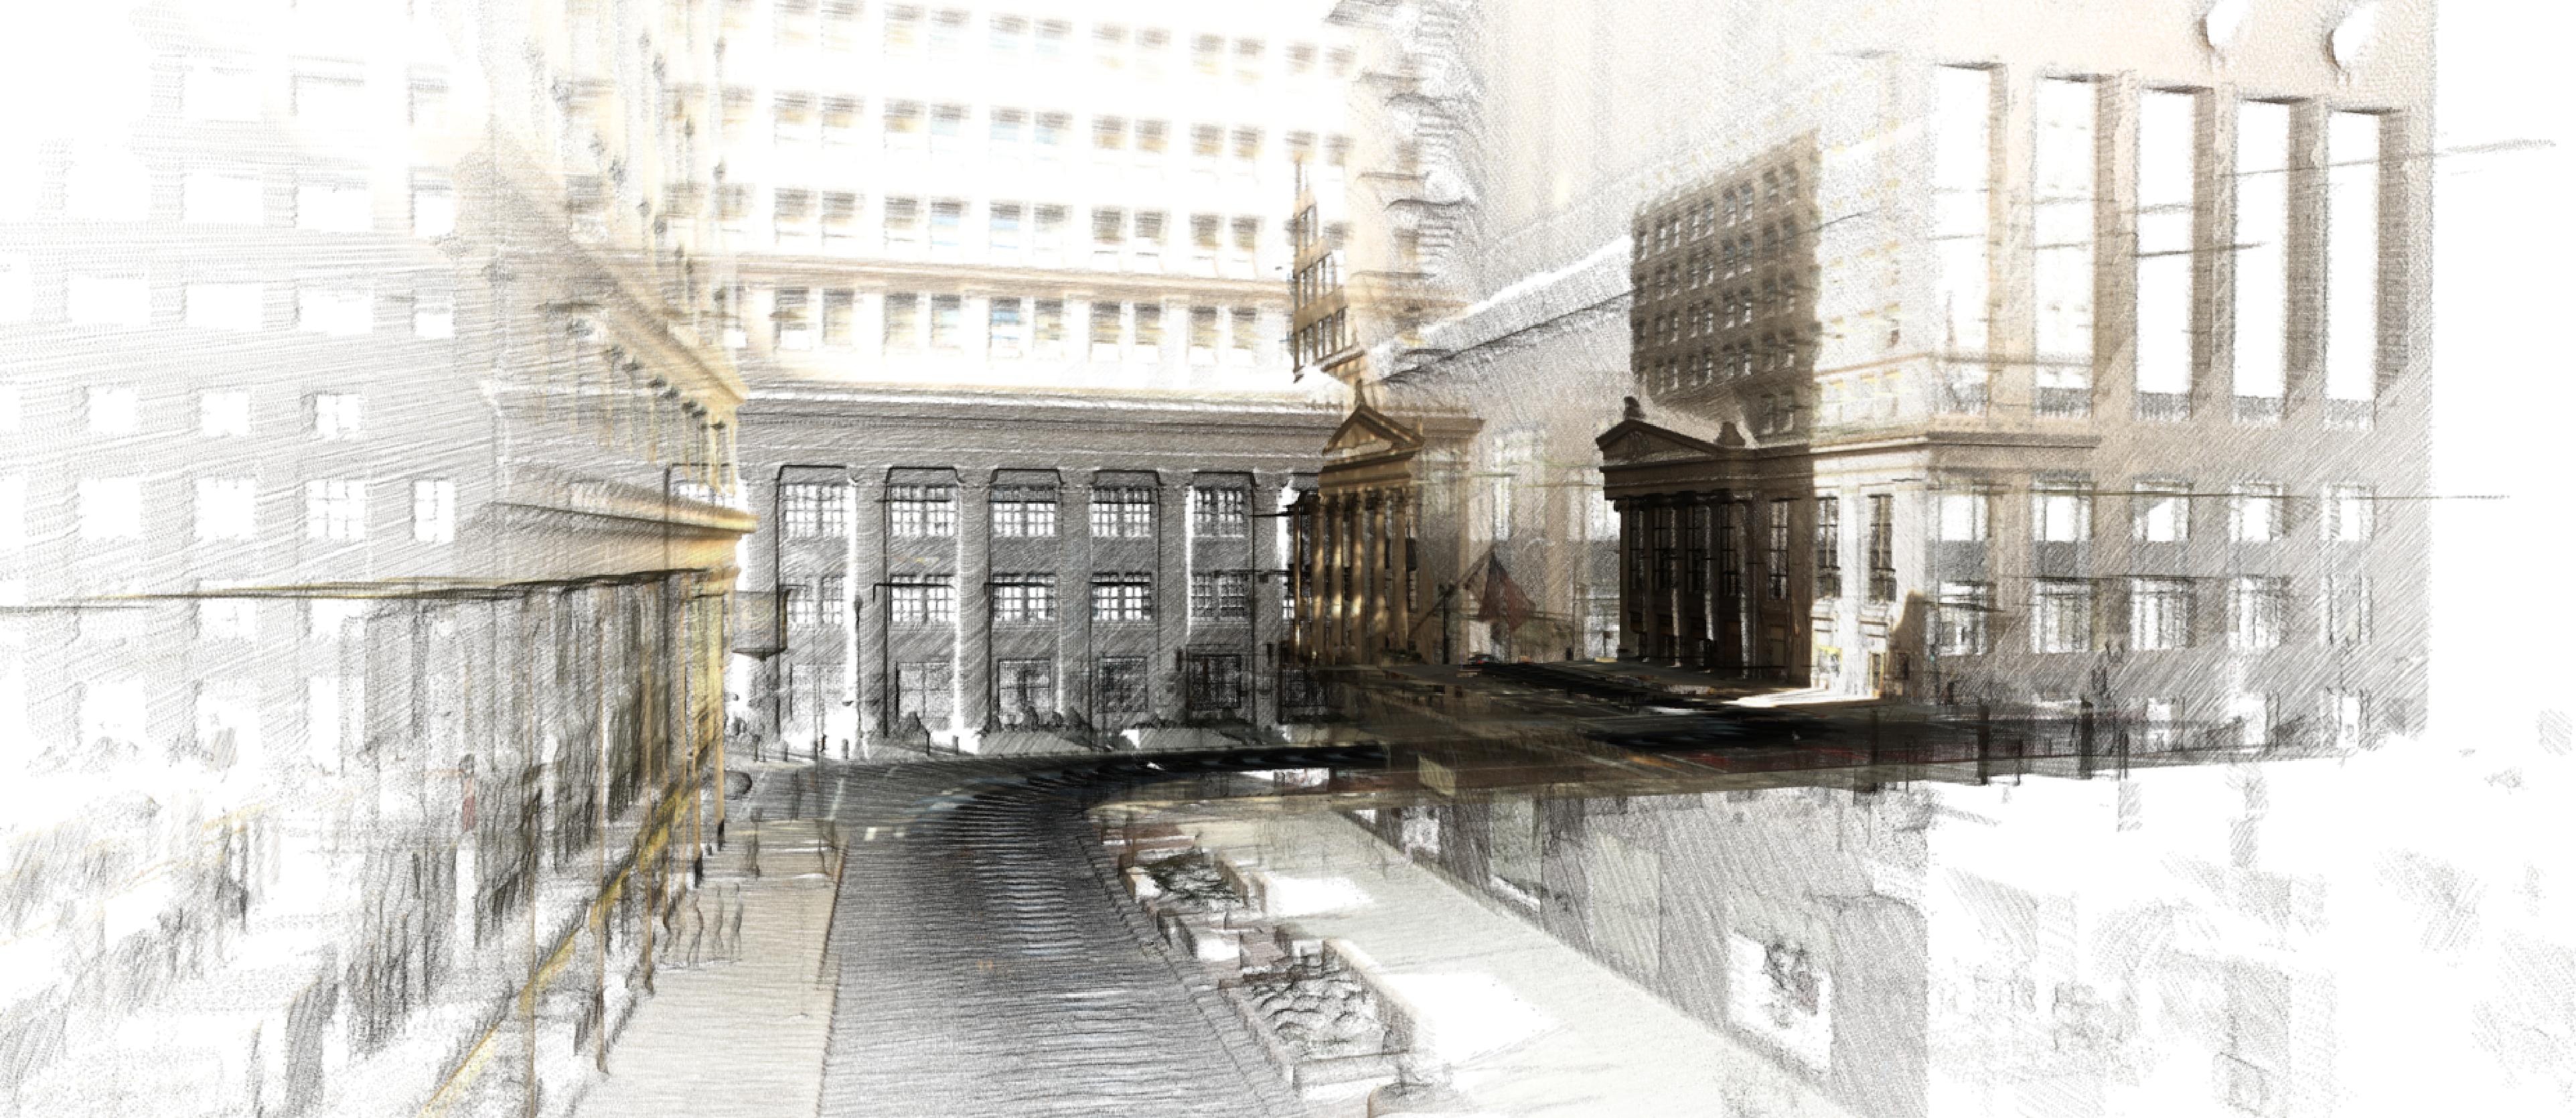
\includegraphics{Pic/PDF/PointCloudLabelling.pdf}}}
\end{tabular}}
\caption{A screen-shot of street view point cloud data used in my research. There are 9195492 points that are contained in this scene.}
\label{fig: point cloud labelling}
\end{figure} 

\Section{The Proposed Solutions} \label{sec: solution}

Data labelling is a tedious and time consuming step of a machine learning process, and may be very expensive especially if experts are involved. To tackle this problem and reduce the cost spent on data labelling, several strategies and techniques had been proposed in last two decades.

A technique that creates synthesized data by over-sampling existing data has been extensively used in computer vision and machine learning. The most popular one among these techniques is SMOTE \cite{CN:02} which over-samples a minority class by using interpolation in feature space. Such interpolation gives a larger and more confident decision region to minority classes. Hence, the learner learns a less-biased boundary between the classes.

Instead of creating new synthetic data, a technique called semi-supervised learning will start from a small amount of labelled data and gradually grow and propagate to get more data labelled. In order to use unlabelled data, several assumption has to be made to the underlying distribution of data, such as: a smoothness assumption, a cluster assumption and a manifold assumption\cite{CO:06}. Under this configuration, semi-supervised learning attempts to use this combination on labelled and unlabelled data were made. The idea is to improve the classification performance by propagating the label of labelled data to unlabelled data so as to expand the set of the data with labels.  

All of the learning schemas and techniques mentioned above have been successfully applied by researchers in the of computer vision and machine learning for decades. However, almost all of these methods are based on an assumption that the distribution of the data is known. Such assumption usually fails unless either a data set with distribution that covers every possibility in feature space is given, which push us back to the problem of data acquisition, or the data of training set and testing set are exactly drawn from the same distribution. An example that can explain this phenomenon is given by the problem of recognizing the human body motion. To have a high accuracy recognition of human body motion, a human body model with high order of degrees of freedom is assumed with each degree of freedom representing a dimension in movement space. If the body movements in training set and testing set are totally different, (say training set containing arm movement only but testing set containing head tuning only), then the learned model has little or even no chance to recognize the testing set. 

In many recognition problems, humans have prior knowledges regarding the structure and the parameter domain of the problem. Take the problem of roof style recognition from satellite images for example, the goal in this problem is to recognize the roof style of a given roof satellite image. The target labels are: hip, halfhip, gable, pyramid, gambrel, and flat. The recognition of the roof style usually is conducted by recognizing features such as ridge lines and valley lines on the roof. However, due to the degradation of image quality and occlusion caused by shadows, it is hard to detect all of these features, the cases of which are shown in Figure \ref{fig: roof edge demonstration}. To solve this problem, since we know how roof is built and we know where those ridge lines and valley lines are located on the roof, hundreds of thousands of synthetic roofs containing these features could be created and then used to train a recognizer. 

Examples of using synthetic data to assist recognition process are very common. The success of these methods and applications lie in the fact that on the one hand, the essential features of an object could be captured by a synthetic model using low level object features, such as the object silhouette, object color and object structure. Thus training a recognizer using synthetic data could capture low level features of objects and can assist the recognition process. A well known application of using a synthetic model for recognition is an object retrieval system in which users are required to provide a rough drawn sketch of underlying target\cite{WC:10}, where the object sketches drawn by the user provide both the silhouette and shape information of an object.

A key problem of using synthetic data for recognition is the mapping between real data and synthetic ones. Reasons for such data mapping come from intrinsic differences between real data and synthetic data. Consider the roof image classification for example, the synthetic roof images are modelled as a parametric model of the combination of the roof's ridges, valleys and corners. By tuning parameters of these elements, we can generate a huge number of synthetic roofs, However by creating synthetic data, it is impossible to simulate numerous possibilities of noisy patterns in real roof images. Therefore mapping is needed to eliminate the gap between real data and synthetic ones. The mapping can be done in many ways and in different stages of the data processing. For the roof case, given a real roof, we need to match it with a synthetic roof so that the different between two is minimal. In addition we need to employ some transformation in feature space to "add" noisy patterns to synthetic data or 'remove" noisy patterns from real data. In this research, I deal with the mapping from both data space and feature space. In data space, I proposed to build a synthetic model that will minimize the distance between real data and synthetic ones. In feature space, since the distribution of the synthetic data is different from the distribution of real data, I consider method that can make a shift for the features of either real data or synthetic data to reduce disparities between the two data. To successfully achieve these objectives I use different computer vision and artificial intelligence  techniques, such as: deep learning and transfer learning.

\begin{figure}[h]
\centerline{
\begin{tabular}{c}
  \resizebox{0.4\textwidth}{!}{\rotatebox{0}{
  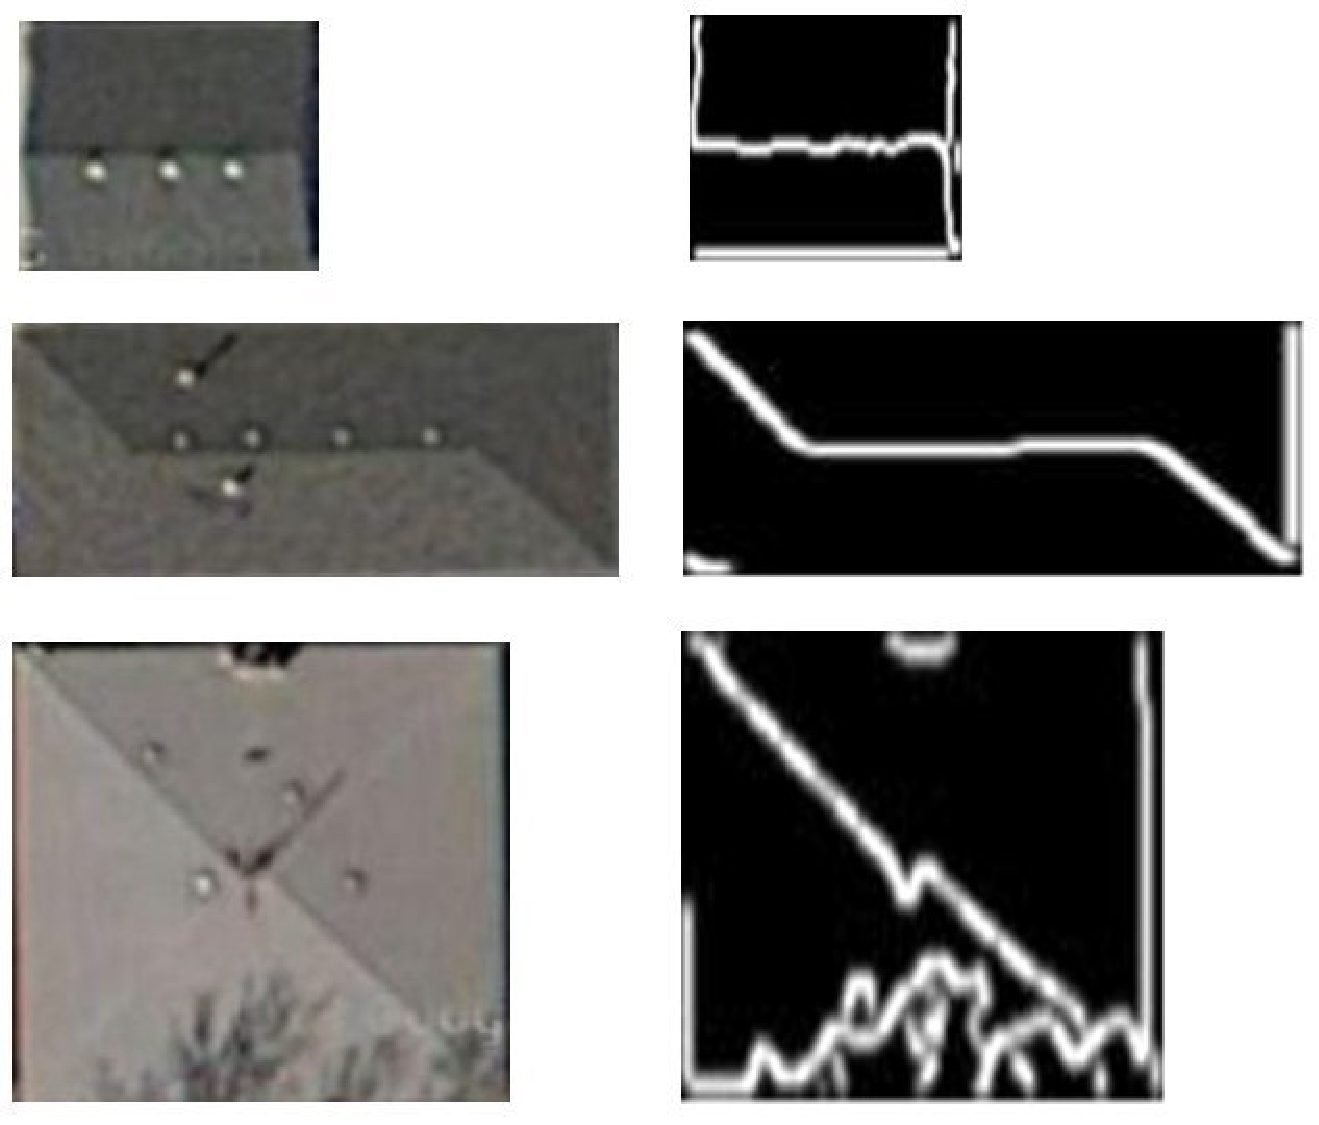
\includegraphics{Pic/PDF/RoofProjectDemo.pdf}}}
\end{tabular}}
\caption{A demonstration of using synthetic template to simulate edge image of roofs used in my research.}
\label{fig: roof edge demonstration}
\end{figure} 

\Section{Novel Contribution} \label{sec: contribution}

%Throughout my doctoral research, we address solving the recognition problem in 2D \& 3D spatial data including satellite images, street view LiDAR and so on. The primary methodology used in my research is learning based methods that solve the recognition problems and improve recognition accuracy by learning from the 2D or 3D artificial templates.
%
%To sum up, the contributions of my research are three folds.
%\begin{enumerate}
%	\item Learning template model from real data. The template model is created as a parametric model of parameters that control the shape and structure of real data. By assuming these parameters follow some certain distribution, to stimulate the real model, the parameters of the template need to be learned from real data. So we can diverse more synthetic models by adjusting these parameters. the challenge in this part is how to identify the correct parameters and range of these parameters from real data.
%	\item Extracting features from data. Discovering highly descriptive features from synthetic data that can be used to recognize real data is very important in the success of my method. Since synthetic data is much more well organized and clean than real data, the challenge in this step is to finding features that can either catch similarity between real data and synthetic data or be discriminative enough to distinguish different object type.
%	\item Using synthetic template model for recognition. Given a repository of synthetic models, a recognizer is built upon the synthetic models. The challenge is to find correct mapping between real data and synthetic ones. To solve the recognition problem, techniques such as deep learning, transfer learning and so on are employed to reduce the difference between real data and synthetic ones.  
%\end{enumerate}

In this researches, I address recognition problems of 2D \& 3D visual data using learning based methods. Generally there are two factors determining the result of a learning process. 

The first factor is the learning algorithm. A successful learning algorithm should be effective and robust to unseen data. The second factor determining the learning result is the data. Data preparation usually is a pre-processing step in machine learning procedures and is often not given enough attention relatively. The quantity and the quality of the data are key factors affecting the success of a learning procedure. 

It is generally accepted that the performance of a learning process could be increased if more data is available. However, data is always not enough. In my research, to solve the lack of data problem, I proposed to use synthetic data to help increase the performance of a learning process. There are various problems when it comes to data synthesis in a machine learning procedure. To sum up, there are two major problems we need to solve. The first problem we has to solve is where to synthesize more data. The word "where" in this context has two meanings. We first should determine in what space to conduct such data synthesis, in data space or feature space. Then we need to determine the location in each space where to add the synthetic data. These are very important questions we should really take care of, because answers to any questions will determine the complexity of the data synthesis process in the first place and the performance of the entire learning process at the end. The second problems deals with how to use the synthetic data in a learning procedure. To simulate actual data in a learning process, the synthesized data has to be as similar to actual data as possible. The synthetic data is useless unless it can truly mimic actual data. To solve these problems, my research has the following primary contributions.

\Subsection{Creation of Synthetic Data in Data Space} Machine learning algorithms usually suffers from lacking of enough training data. In existing methods researchers usually use a technique called data augmentation to increase the amount of training data. In data augmentation, new examples are generated as a perturbed version of the original data. Take image augmentation for example, to augment new images, the original images are stretched, added noises or partially cropped from the original images. Images generated in this way form a distribution in parameter and feature space which is centered at the original images. Thus, these new images do not introduce much new informations in this case. Therefore, the learner may fails to learn a more general decision boundary from the resulting data and the increase in performance will be limited.

In my research, to better simulate actual data, a series of methods that synthesize more data are introduced. These methods can be basically separated to two groups. In first group, different from existing methods, my methods of data synthesis are based on usage of a centralized representation of actual data. We call such centralized representation a prototype in this proposal, because the prototype can characterize the most essential structures and patterns of actual data. The prototype in my work is modelled as a parametric model of control points and could be learned using semi-automatic or automatic approaches. Using technique such as interpolation between existing data and randomly drawing synthetic data from a distribution computed from control points of existing data, more data could be synthesized easily. Methods in second group are machine learning based methods, along the recent year' development of deep neural network, especially in computer vision area. Large dataset has become a necessary input to neural networks to gaurantee a desired performence of the neural networks.  Image level or even pixel level data synthesis become even valuable and important in these tasks. In my work, depending on learning and computational power of deep neural networks, I explored and proposed ways that synthsize image level data by letting neural network learn existing data. The synthesized data whose usage is demenstrated in application such as data retrievel, object tracking and so on.

The proposed approach has been used in many object recognition problems in my research. The preliminary results can be found in \cite{Zhang2014Autoencoder}\cite{AndiZang2015}\cite{ZX:14}.

\Subsection{Learning From Synthetic Data} Directly using and learning from synthetic data may cause failure or a classification results with poor performance, even though there is enough synthetic data. This is because, the synthetic data is generated using a data prototype(parametric model) which is a simplified version of data representation. Since there is no way for a prototype to generate information such as noise and some other complicated patterns of actual data, this results in nonequivalence in terms of information contained by features computed from actual data and synthetic data. Thus synthetic data holds a different decision region with respect to actual data and the result may be poor classification performance if learned directly from these data. 

A general goal of feature extraction is to minimize the difference between actual data and synthetic data by using extracted features. To achieve this goal, I propose two strategies in feature extraction that prove to be useful. First, extracted features have to be able to capture the most essential characteristics between actual data and synthetic data, thus ignoring noise all the noises and inherent patterns. Second, extracted features should be able to compensate for such additional information for synthetic data. Under these two directions, several techniques and algorithms are developed in this work.

The preliminary results of the proposed feature extraction strategies could be found in \cite{Zhang2014Autoencoder}\cite{AndiZang2015}\cite{ZX:14}.

%Feature extraction especially extracting good features is acrucial step in every machine learning algorithm. Although some machine learning algorithm could select most distinguishable features automatically. Good features not only better distinguish the characteristics of different objects, they ease and speed up the learning process as well. Feature extraction becomes even challenging and harder in terms of capability of distinguishability When synthetic data is introduced in a learning process. Because on the one hand, features extracted from synthetic data have to recognize the actual data that are in a same class as synthetic ones. On the other hand, features must be still different enough for objects in different classes.
%
%So far as we know, most of existing works treat synthetic data and actual data equally and few works invent their own features for the purpose of learning from synthetic data. In my research, for different project including object matching, object classification and recognition and for different types of data including images, point clouds, many new features are invented. These features are generated to minimize the difference between synthetic data and real data that are similar and in the same class while still discriminative enough in separating data of different classes. 

\Subsection{Elimination of Synthetic Gap} Learning a classifier from synthetic data is extremely hard, due to the following reasons. First, using a prototype to synthesize more data causes the distribution of the generated data to shift away from that of actual data. We term such distribution shift as \textit{synthetic gap} in this proposal. The \textit{synthetic gap} is a major obstacle in learning from synthetic data, since synthetic data may fail to simulate the potential useful patterns of real data for training classifiers. Second, since practically a small amount of labelled data may be available, it is necessary to jointly learn from synthetic and real data. The learning process must be automatically leveraged between the synthetic data and the real data. 

Different from existing work, here we solve the problem from a more general perspective by eliminating the \textit{synthetic gap} as a domain adaptation problem. A general framework based on a neural network with novel architecture is proposed. The neural network is trained as a regressor which could map synthetic data to real data and find out the potential transformation between two types of data. Thus it is able to close the gap between two data. With this mechanism synthetic data could better simulate actual data and used in a machine learning procedure.


%Designing features that extracts the most essential structure and knowledge from both actual data and synthetic data achieves good results in learning algorithm. However, we notice in my experiments that in some situation, there still exists inevitable differences between features extracted from two kinds of data. We name this type of difference as: synthetic gap. Learning from a synthetic dataset that has synthetic gap will cause learning method biased to synthetic data thus result in a low accuracy in recognizing actual data. 

%To minimize or even eliminate the gap, a general framework based on a neural network with novel architecture is proposed. The neural network is trained as a regressor to automatically find out the relationship between two types of data, thus is able to close the gap between two data. With this mechanism synthetic data could better simulate actual data and used in machine learning procedure.

\Subsection{Creation of Synthetic Data in Feature Space} Quality of datasets play an important role in machine learning. Somebody even say the dataset is the root of a successful machine learning method. However, in practice, many applications and machine leanring problems suffer from degraded performance due to unbalanced distribution of datasets.

Data synthesis through prototype can be used to improve performance of many applications suffering from unbalanced data distribution. However, due to the nature of the methodology, it is limited to some specific problems.  A more general solution is to directly create synthetic data representation to achieve a balance in its feature space. 


Synthesizing new data in feature space is hard. Because data representation in feature space is abstract that the actual meaning of the data in data space is hard to interpret. To know where to synthesize new data so as to balance the data distribution and improve the performance of underlying machine learning tasks such as classification, it requires a deep understanding of distribution of entire dataset. To achieve this goal, I proposed a theorotically gauranteed minority oversampling algorithm which takes both data distribution of minority and majority class into account and can synthesize data to achive better classification results compared to existing methods. Details of the algorithm could be found in Chapter \ref{chapter: feature space}.

\clearpage

\Chapter{Creation of Synthetic Data in Data Space} \label{chapter: data space}

\Section{Introduction} \label{dataspace: introduction}

It is generally accepted that an accurate classifier can be learned if a large and balanced labeled training dataset is available. In real-world scenarios, however, one always struggles to find adequate amounts of labeled data. Even with the help of crowdsourcing, e.g., Amazon Mechanical Turk (AMT), it is often difficult to collect a large quantity of labeled instances with high quality that is necessary for training a classifier for a real-world problem. In terms of quantity, it has been shown that amount of available training data, per class, follows Zipf distribution \cite{torralba2011app_share}. In terms of quality, some domains, such as analysis of satellite images(e.g. the comet images from Rosetta), require extensive and detailed expert user annotation \cite{remotesensing2013}. Large volume of LiDAR point cloud data have to be labeled before they can be used to train some classifiers \cite{ZX:14}. Such labeling process usually is very time consuming and requires expert-level labeling efforts or expensive equipments. Practically only a very limited portion of the data points can be obtained. The fundamental issue of learning from not enough data is the ability of these data to significantly compromise the performance of most standard machine learning algorithms. Most standard learning algorithm, generative and discriminative, assume that enough knowledges and features could be extracted from training data that have a balanced distribution. Therefore, when presented with a complex dataset but with less amount of data, these algorithms fail to properly represent the distributive characteristics of the data and resultantly provide unfavorable accuracies.

Technically, there is no official definition or a quantitative measure about rare data learning. It is important to understand rarity of different forms. According to \cite{Weiss}, rarity could comes from either relative rarity which is usually related to imbalanced learning or absolute rarity which is a direct result of the nature of the data set. my method and solution partially overlap with imbalanced learning in cases when data is imbalanced distributed, and the minority classes are viewed as rare data. More than rare data learning, methods discussed in this chapter solve more general problems in which labelling actual data maybe is very time consuming or a job must need a lot of labor works to be done. 

I propose to create synthetic data and use them to solve mentioned problems in a machine learning process. The idea of using synthetic data in machine learning algorithm has a long history and is associated with the development of cognitive psychology, artificial intelligence and computer vision. The reason simply lies in the facts that first creating synthetic data is much easier when actual data could be represented as a parametric model. Second, if I view a class of objects in data space as a whole, synthetic data and actual data are both subsets of the entire dataset which may or may not overlap. Indeed synthetic data is no more than an ideal representation of actual data. As an example, I show edge images extracted from my satellite roof top images and its corresponding synthetic images in Figure \ref{fig: roof real and synI}. It could be observe from this figure that actual images are highly similar to synthetic ones and could be identical to synthetic ones if noises can be removed.

\Section{Related Work} \label{dataspace: relatedwork}

Due to technical constraint in five years, data synthesis is limited to just using geometrical transformation and degradation models. In \cite{VT:03}\cite{VT:04}, to help off-line recognition of handwritten text, a perturbation model combined with morphological operation is applied to real data. They showed that when a moderate transformation is added to the real data, the resulting synthetic training set boost the performance. Synthetic data generation techniques has been moderately implemented in area of optical character recognition. in \cite{NJ:09}, researches and experiments were conducted to test the safeness of using synthetic data in machine print text recognition problem. Following the conventional way of generating synthetic data, they model each synthetic data as a geometrically transformed version with different magnitude of the original data. They demonstrated that classifier trained on interpolated data often but not always improved classification when tested on previously unseen samples. However, the use of interpolated data in the training sets has never worsened the results. To enhance the quality of degraded document, in \cite{BG:08} degradation models such as brightness degradation, blurring degradation, noise degradation and texture-blending degradation were used to create a training dataset for a handwritten text recognition problem. The synthetic minority oversampling technique (SMOTE) \cite{CNV:02} and its variants \cite{HH:05}\cite{HH:08} are also powerful methods that have shown many success in various applications.  However, these previous methods are relatively limited to one particular type of dataset, whilst  I propose a more general  methodology of generating synthetic data by creating a parametric prototype of the data. By tuning parameters of the prototype, my method can derive synthetic data that cover almost all possibilities. A very interesting work whose intention is a bit similar to mine is proposed in \cite{Pauly:2004:UVP:2386332.2386346}. In this paper, to analyse variability in point-sampled geometry, authors first assume every data comes in with incomplete information about ground true object. They then capture this uncertainty by introducing a statistical representation that quantifies for each point in space the likelihood that a surface fitting the data passes through that point. This likelihood map is constructed by aggregating local linear extrapolators computed from weighted least squares fits. The quality of fit of these extrapolators is combined into a corresponding confidence map that measures the quality of local tangent estimates.

In recent five years, along with the development of deep learning techniques. Research of data synthesis, particularly image synthesis, has receive more and more attention. There are two reasons for this phenomenon. On the one hand, large deep learning system usually need large amount data to gaurantee a unbiased and high quality model (network/networks), which make desire for synthetic data become more imperative. On the other hand, modern deep learning techniques provide a efficient and prominent way to synthesize data. 

Many efforts have explored using synthetic data for various prediction tasks, including gaze estimation \cite{wood2016learning}, text detection and classification in RGB images \cite{gupta2016synthetic}, font recognition \cite{wang2015deepfont}, object detection \cite{gupta2014learning}, hand pose estimation in depth images \cite{tompson2014real}\cite{supancic2015depth}, scene recognition in RGB-D , semantic segmentation of urban scenes \cite{ros2016synthia}, and human pose estimation 
\cite{park2015articulated}\cite{shakhnarovich2003fast}\cite{lecun2004learning}\cite{ionescu2014human3}\cite{pishchulin2012articulated}\cite{rogez2016mocap}.  Gaidon \cite{gaidon2016virtual} show that pre-training a deep neural network on synthetic data leads to improved performance.

Due to a technique called Generative Adversarial Network (GAN) introduced by \cite{goodfellow2014generative}, Generating complicated deceptive artificial images become truly possible. Basically, the GAN framework learns two networks (a generator and a discriminator) using competing loses. The goal of generator network is to map a random noise to realistic images so as to fool discriminator network, whereas the goal of the discriminator network is to distinguish the generated from the real images. Since introduction of GAN, many extended works have been proposed for data synthesis purpose \cite{salimans2016improved}. Based on several improvements on basical GAN network structure, Radford \cite{radford2015unsupervised} proposed a network framework that could synthesize much more realistic images. Li and Wand \cite{johnson2016perceptual} proposed a Markovian GAN for efficient texture synthesis. Lotter use adversarial loss in a LSTM network for visual sequence prediction. With auxiliary classifiers added to GAN model, \cite{odena2016conditional} investigate performance of variants of GAN models on image synthesis task. By using two GAN models in a cycle framework, cycleGAN \cite{zhu2017unpaired} is able to acheive image style transfer. Later, a conditional cycleGAN is introduced in \cite{lu2017conditional} for more specific image synthesis tasks. In my work, I proposed to synthesize realistic image using image descriptions. The earlist work of this task could be back to \cite{mansimov2015generating}, although no GAN is used in this work, by using recurrent neural network, this work found the basic framwork of text to image transfer. Combining GAN and text features generated from a LSTM, \cite{reed2016generative} could parse image description to synthesize realistic image corresponding to the description. The same idea is found in \cite{DBLP:journals/corr/DongZMG17}, however, LSTM is co-trained with GAN in this work. A stackedGAN structure is proposed in \cite{zhang2016stackgan}, due to image quality refinement broght by second GAN in this stacked-up structure, the network is able to synthesize highly realistic images.


\Section{A Brief Introduction of Proposed Methods} \label{dataspace: solution}

In my approaches, I create synthetic data in data space. Creating synthetic data in data space has several advantages. First, it is the most intuitive way to create new data, because it is easy to judge the quality of the new data. Second, creating data in data space let us understand my data more clearly and deeply, because in order to create new data, I have to understand the characteristics and structure of original data. Having these understanding, it is more likely I will invent some better features that would boost the performance of machine learning process later on. The feasibility of my method is based on an observation that data of most problems can be converted to a parametric model, in my cases 2D and 3D models controlled by multiple control points. By adjust values of parameters I are able to derive many synthetic data. 

In my research, the approach of creating synthetic data in data space primarily solves two types of problems. First, by creating more synthetic data, I solved problems of rarity learning. Because as I mentioned that both actual data and synthetic data are subset of entire dataset. By creating massive number of synthetic data, the approach enriches and compensates the part in data space where actual data does not reach, so that a more complete distribution of the data and a more tight boundary between classes of data are provided to machine learning algorithm to learn. Second, for some problems, using synthetic data will greatly reduce labor works spending on labelling actual data. Because instead of label huge number of actual data, using my method, by indicating a label of data, I can generate as many as possible synthetic data I need. For these two problems, I will use the rest of this chapter to discuss the details of creating synthetic data in my previous works. Also, I am going to talk about the problems and challenges in my future research.at the end of this chapter.

\begin{figure}
\centerline{ %
\begin{tabular}{cc}
\resizebox{0.48\textwidth}{!}{\rotatebox{0}{
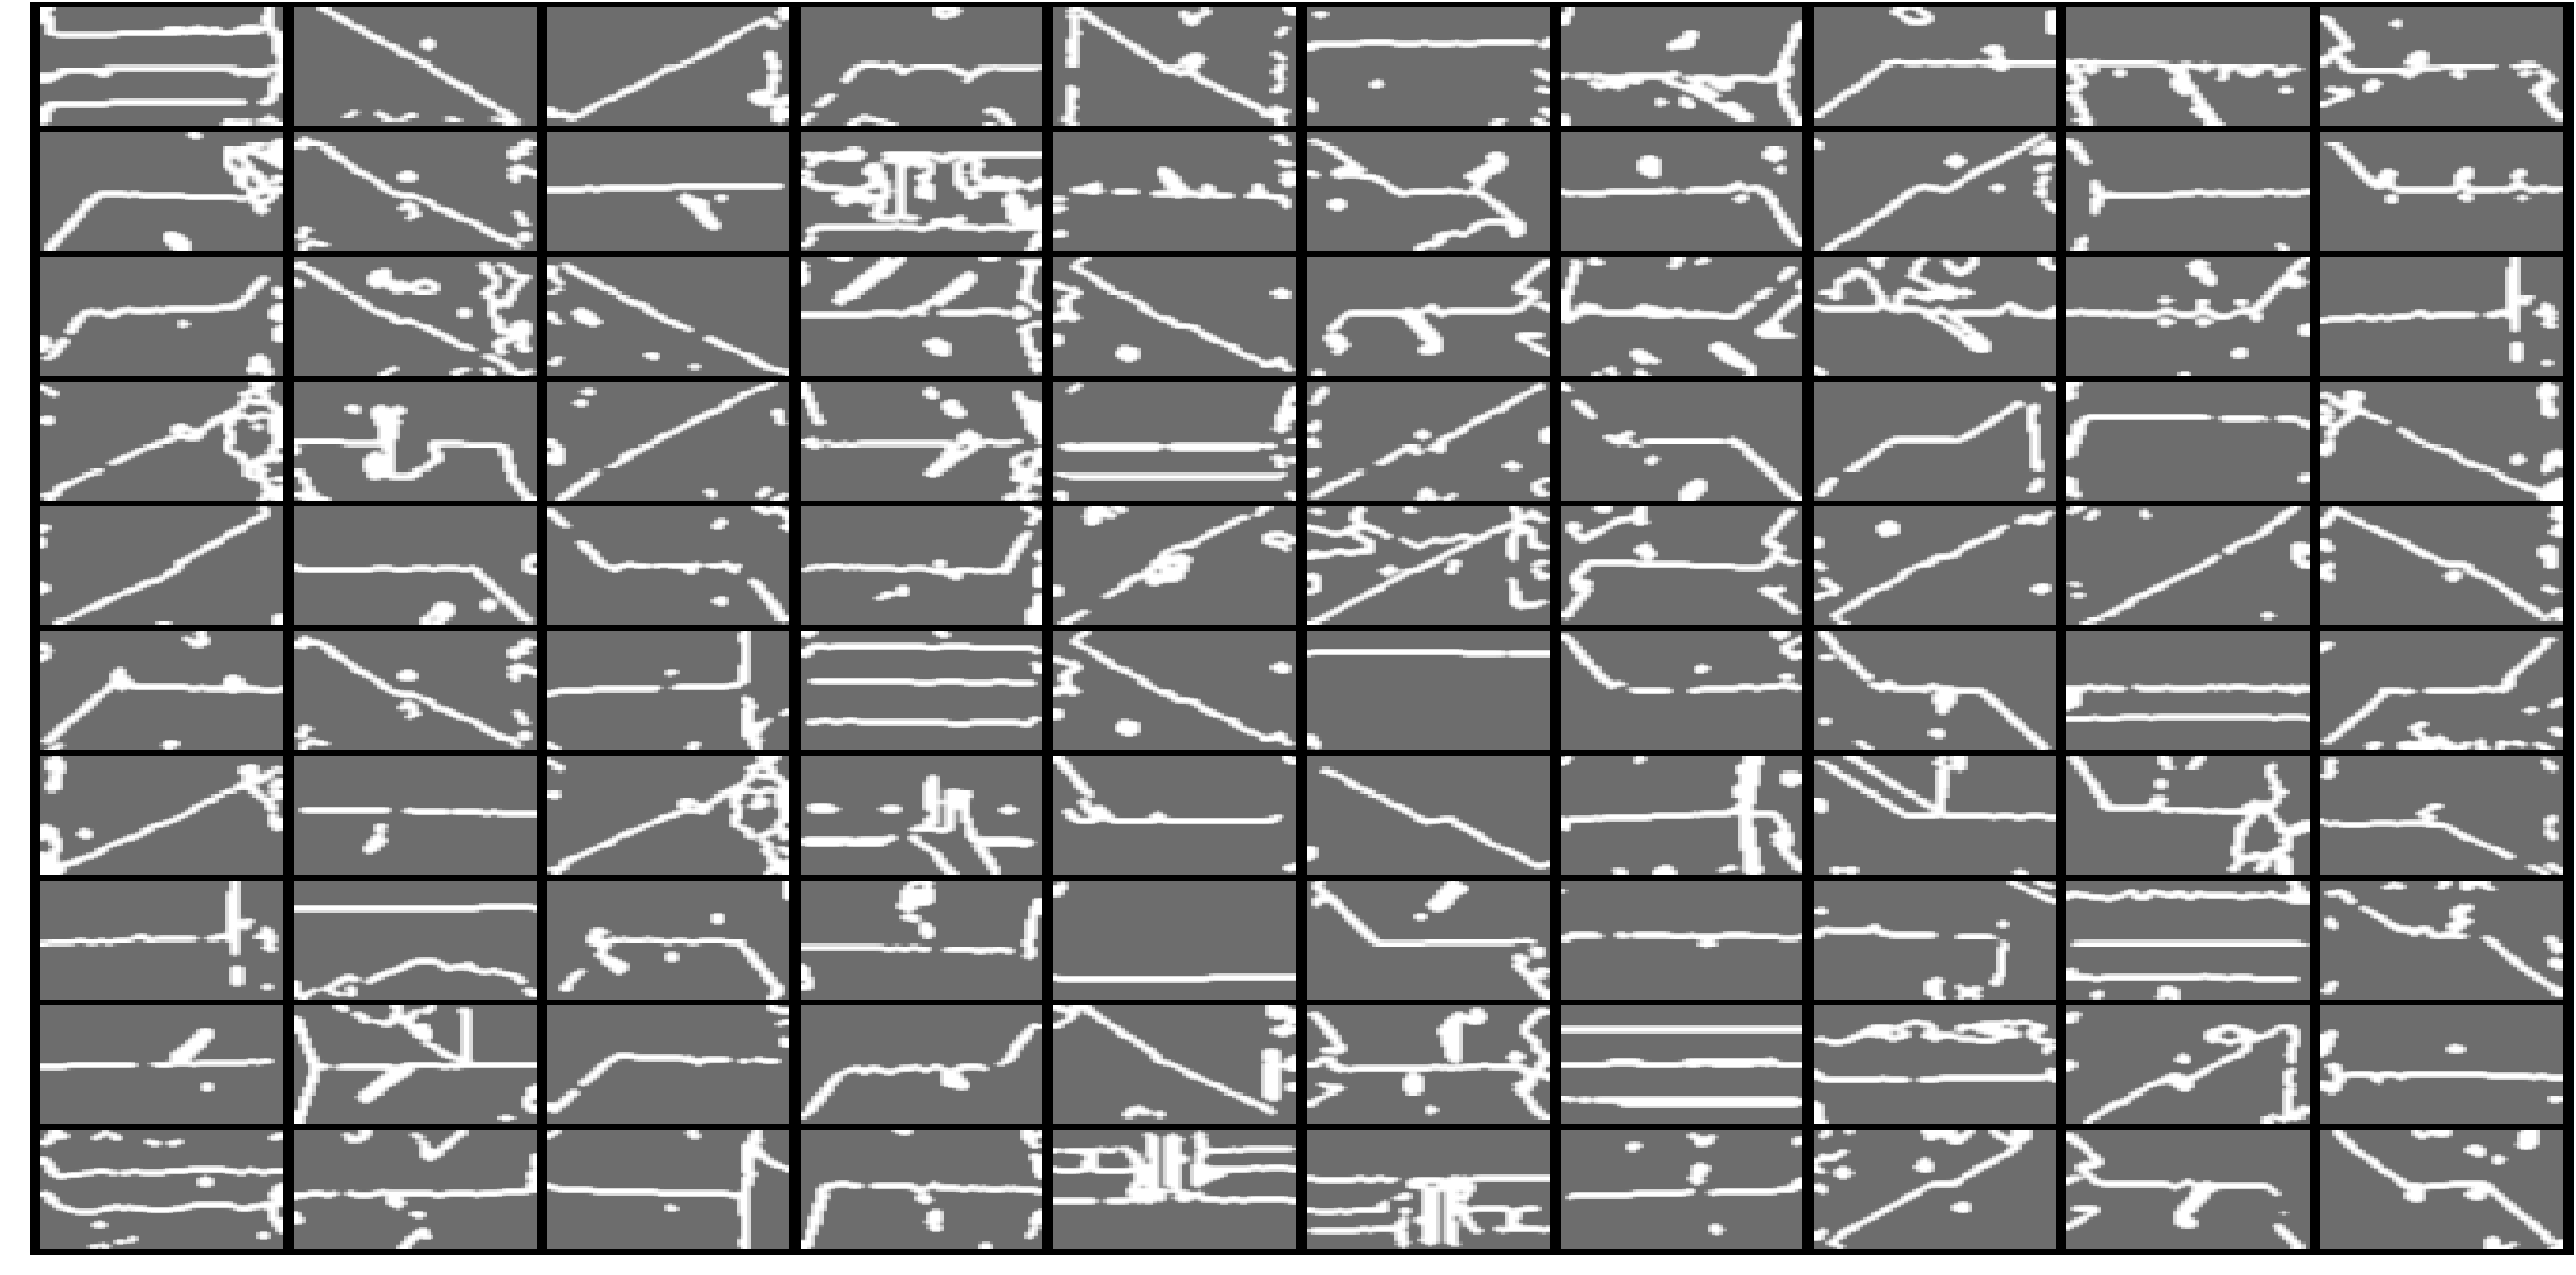
\includegraphics{./Pic/PDF/RealSamples.pdf}}}  
&
\resizebox{0.48\textwidth}{!}{\rotatebox{0}{
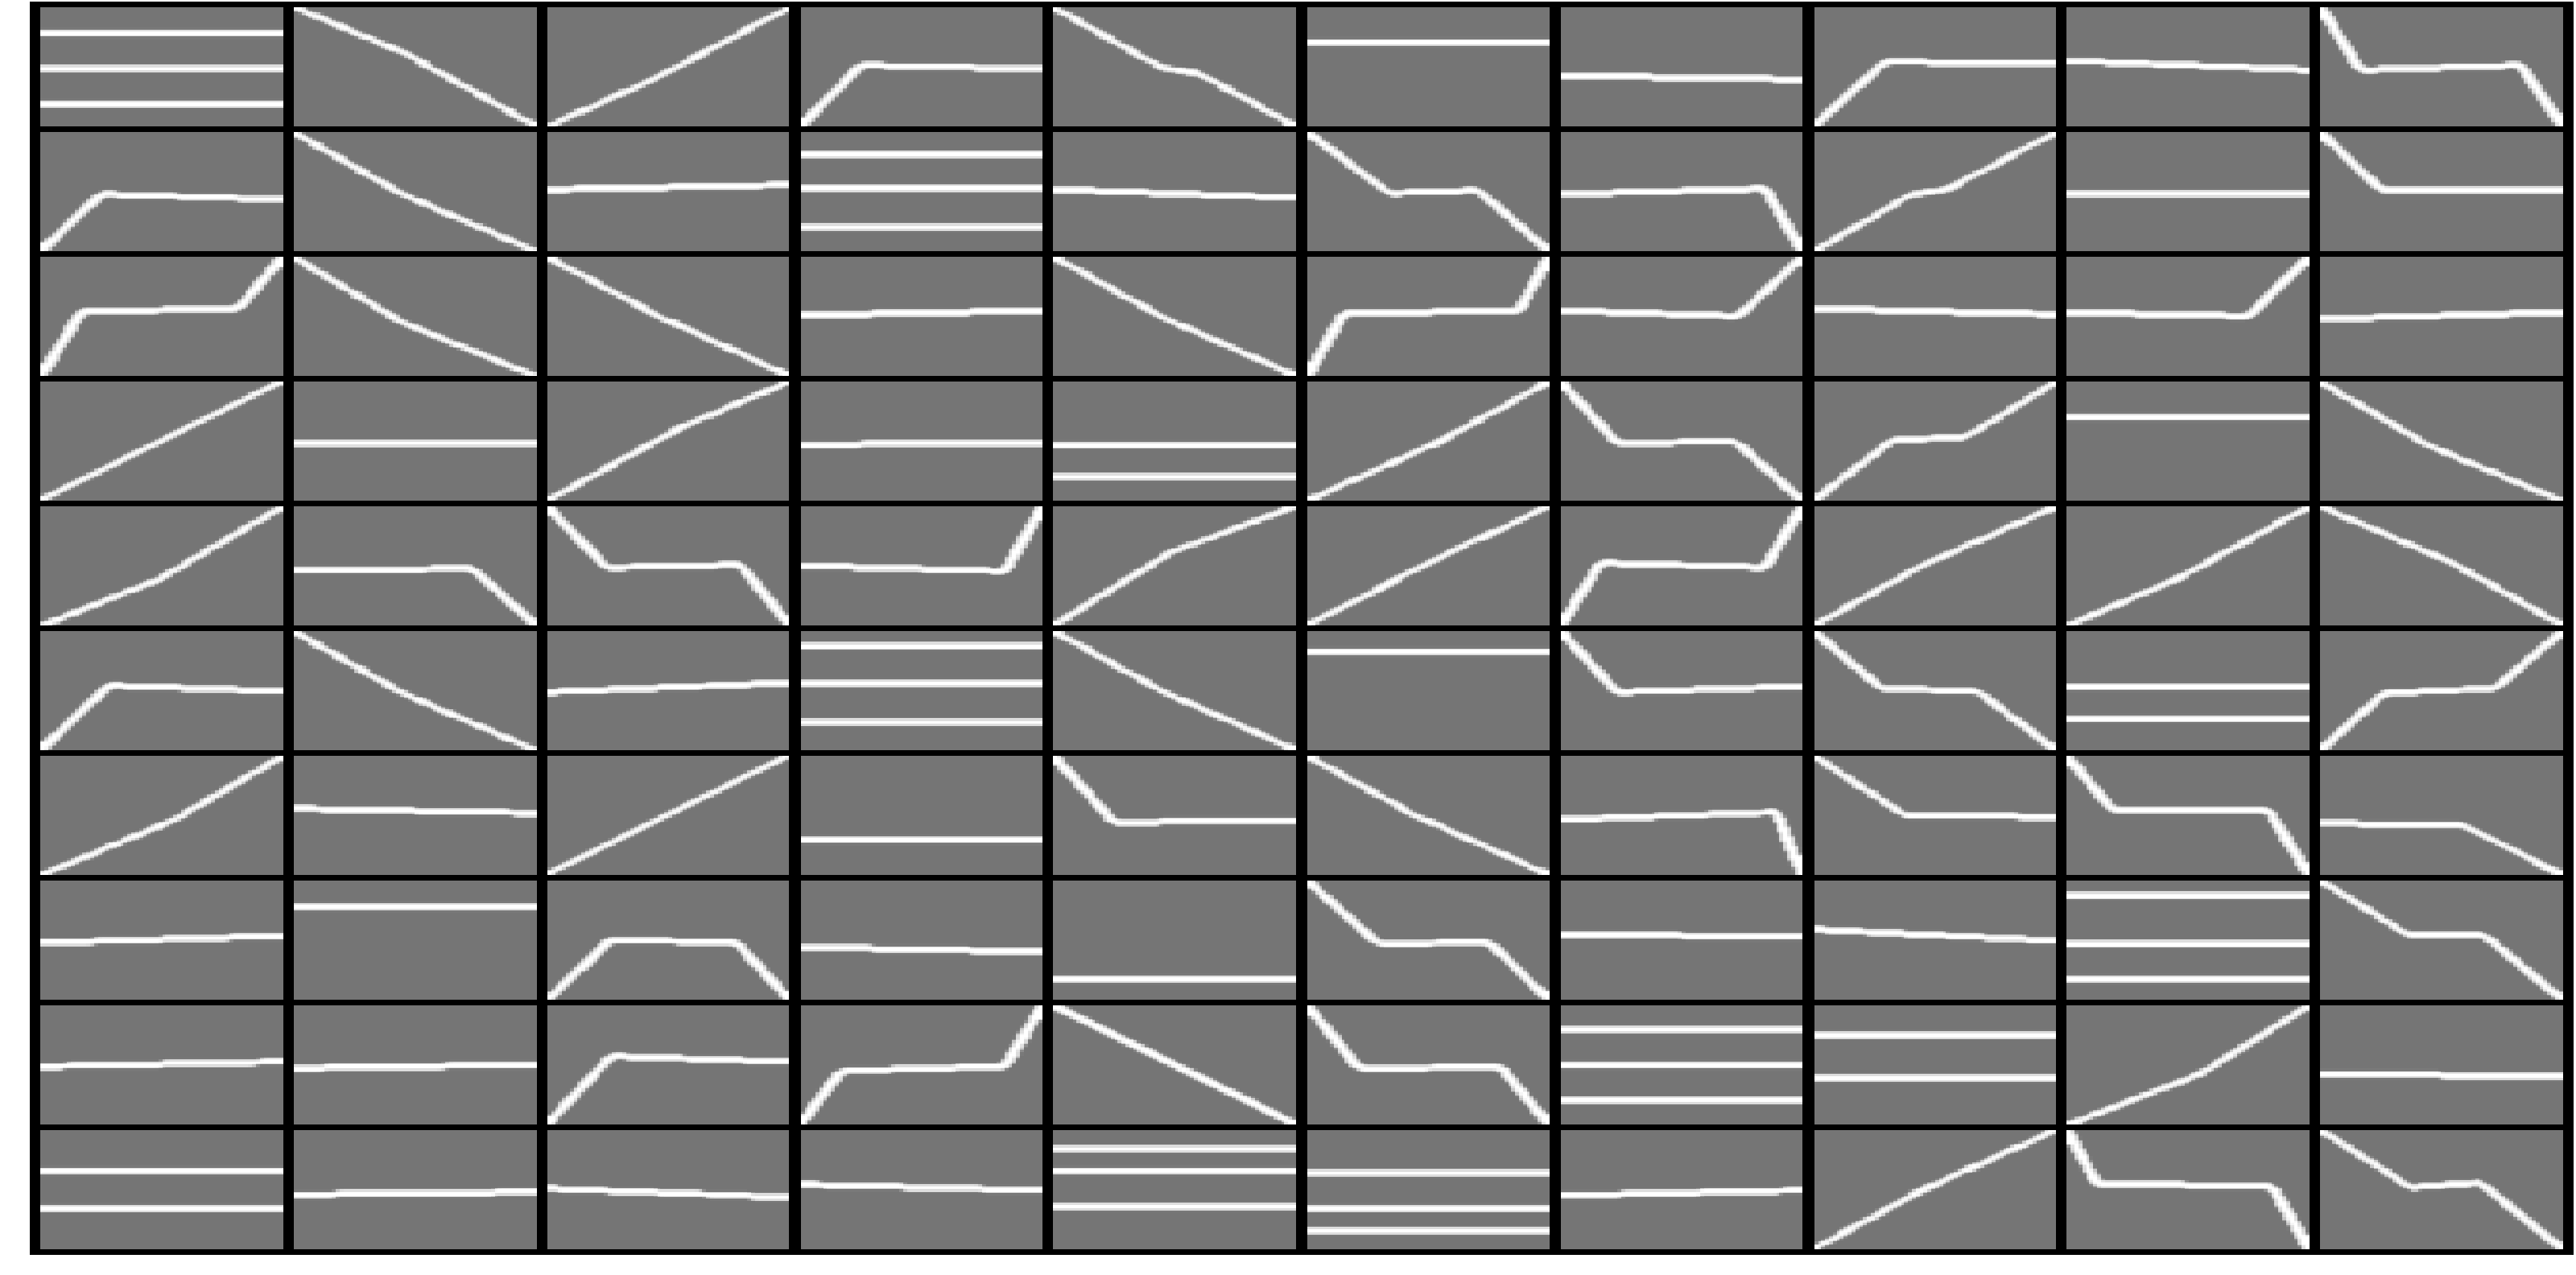
\includegraphics{./Pic/PDF/TmpltSamples.pdf}}} 
\\
(a) Real roof edges & (b) Synthetic roof edges 
\\
\end{tabular}} 
\caption{Examples of (a) real roof edge vs. corresponding (b) synthetic roof
edge images. The synthetic data is generated by the algorithms in Sec.
4. The examples are randomly drawn from SRC dataset.}
\label{fig: roof real and synI} 
\end{figure}

\Section{Creating Synthetic Data to Avoid Rarity Learning} 

Learning from rare data is very challenging, because rare data are typically much harder to identity than common data and most standard machine learning algorithms have a great deal of difficulty to detect regularities within the rare data.

Generally, there are two types of rarities in context, Much of the research on rarity relates to \textit{rare classes}, or more generally, class imbalance. This type of rarity requires labeled examples and is associated with classification problems. A second type of rarity concerns \textit{rare cases}. Informally, rare cases  correspond to a meaningful but relatively small subset of the data, or equivalently, define a small region of the instance space. Rare cases depend only on the distribution of data and therefore are defined for both labeled and unlabeled data, for supervised and unsupervised data mining tasks. Rare cases are naturally defined by the domain and will share common characteristics. In the case of labeled data, a rare case corresponds to subconcept, or subclass, that occurs infrequently. 

There are a number of problems that arise when mining rare classes and rare cases. The first problem I could encounter is lack of data. In this case, the number of examples associated with the rare class is small in an absolute sense which make it difficult to detect regularities within the rare classes/cases. Another problem could that could happen is generating a learning model by using an inappropriate inductive bias. Generalizing from specific examples, or induction, requires an extra-evidentiary bias. Without such a bias "inductive leaps" are not possible and learning cannot occur. The bias of a data mining systems is therefore critical to its performance. One more difficulty comes with noise in training data, especially when rare classes/cases are associated with noise. Since noise data will affect the way any data mining system behaves, but what is more interesting in my research is that noise has greater impact on rare cases that on common cases. Because rare classes have fewer examples to begin with, it will take fewer "noisy" examples to impact learned subconcept. In this case, the learner cannot distinguish between exceptional (rare) cases and noise.

Among all of these challenges and difficulties, in my research, I primarily deal with supervised classification problem which may have \textit{rare classes} or \textit{rare cases} or both. By synthesize more data to create a much more balanced training set using my techniques, I demonstrate that a better performance could be obtained in many classification problems.

\Subsection{Satellite Image Roof Style Classification} Recognizing building roof styles is an important step in many applications including building reconstruction and urban planning. Such problems generally need very high quality training data. However, there is no previous dataset for such problem. Usually collecting data through online crowdsourcing, e.g., Amazon Mechanical Turk (AMT) is very expensive. So to facilitate the study, in my works \cite{AndiZang2015}\cite{Zhang2014Autoencoder}, a few volunteers are invited to join the project and manually crop images from civilian level online digital maps. Manually cropping images is an tedious and time consuming task. By the end of data collection, I are able to only crop a few thousands of roof images. 

{\linespread{1.5}
\begin{algorithm}[ht]   
	\caption{ Footprint Segmentation}   
	\label{alg: 1}   
	\begin{algorithmic}[1] 
		\REQUIRE ~~\\
		The set of footprint vertices, $V$; 
		\ENSURE ~~\\  
		The set of selected segmented region vertices sets, $S$; 
		\STATE Initial $S$;  
		\STATE PUSH($V$, $S$); 
		\IF{$\arrowvert V \arrowvert > 3$}
			\FOR{$i = 1$ \TO $ \arrowvert V \arrowvert$}
				\IF{$V_i$ is POI}
					\STATE Calculate cutting line $\{V_i, D\}$, where $D$ is the other endpoint;
					\STATE PUSH ($\{V_i, D\}, C$);
				\ENDIF
			\ENDFOR
			\FOR{$i = 1$ \TO $\arrowvert C \arrowvert$}
				\FOR{$j = 1$ \TO $ \arrowvert S \arrowvert$}
					\STATE POP ($R$, $S$), where $R$ is the top element in $S$;
					\STATE Cut $R$ by cutting line $C_i$ into $R_1$ and $R_2$;
					\STATE PUSH ($R_1$, $S$);
					\STATE PUSH ($R_2$, $S$);
				\ENDFOR
			\ENDFOR
		\ENDIF   
		\RETURN $S$; 
	\end{algorithmic}  
\end{algorithm}  
}

For a large building which is usually comprise of multiple parts, I even develop an algorithm that reasonably segment large roof image to simple parts. I design an algorithm to decompose complex footprint. The basic idea of this algorithm is to segment the concave footprint into several convex polygons, while the cutting line should make the new polygons have less sum of variances of all inner angles in them. The reason I want to use convex polygon rather than concave polygon to recognize is generally the roof styles can be built on convex polygon much easier. 

To achieve this, I assume the vertex whose inner angle is larger than π as point of interested (POI). Then I need to traverse all possible angles from POI and find which cutting line leads the minimum variance of all inner angles in this segmentation. With calculated cutting lines and given footprint vertices, I can segment the polygon into basic parts. The algorithm shows in Algorithm \ref{alg: 1}, Let $V$ be the set of footprint vertices, which elements has been sorted in clockwise or counterclockwise, $S$ be the set of selected segmented region vertices sets while $S$ is a queue. $C$ is the set of cutting lines. $R$ is a set of polygon vertices and $R_1$, $R_2$ are the segmented polygon vertices.

The cutting line calculation follows:

\begin{equation}
\sigma(i)= \sum_{j=1}^{2} \sum_{k=1}^{\arrowvert A_jP \arrowvert} [{A_{jP(i)}(k)- \frac{(\arrowvert A_jP \arrowvert-1)\times \pi}{\arrowvert A_jP \arrowvert}} ]
\end{equation}

Where $i$ is a given cutting line, $P(i)$ is the set polygons which generated by cutting line $i$. $A_jP$ is the set of inner angles of $j^th$ polygon in set $P$. Hence the appropriate cutting line should be $\argmin(\sigma)$, while $\sigma(i)$ is the set of variance of cutting line $i$. The time complexities of cutting line calculation and polygon segmentation are constants. Hence the total theoretical maximum time complexity is $Ο(\arrowvert V \arrowvert+2^{\arrowvert C \arrowvert})$, while $2^{\arrowvert C \arrowvert}$ always has same magnitude with $\arrowvert V \arrowvert$.

\begin{figure}[htb]
	\centerline{
		\begin{tabular}{c}
			\resizebox{0.6\textwidth}{!}{\rotatebox{0}{
					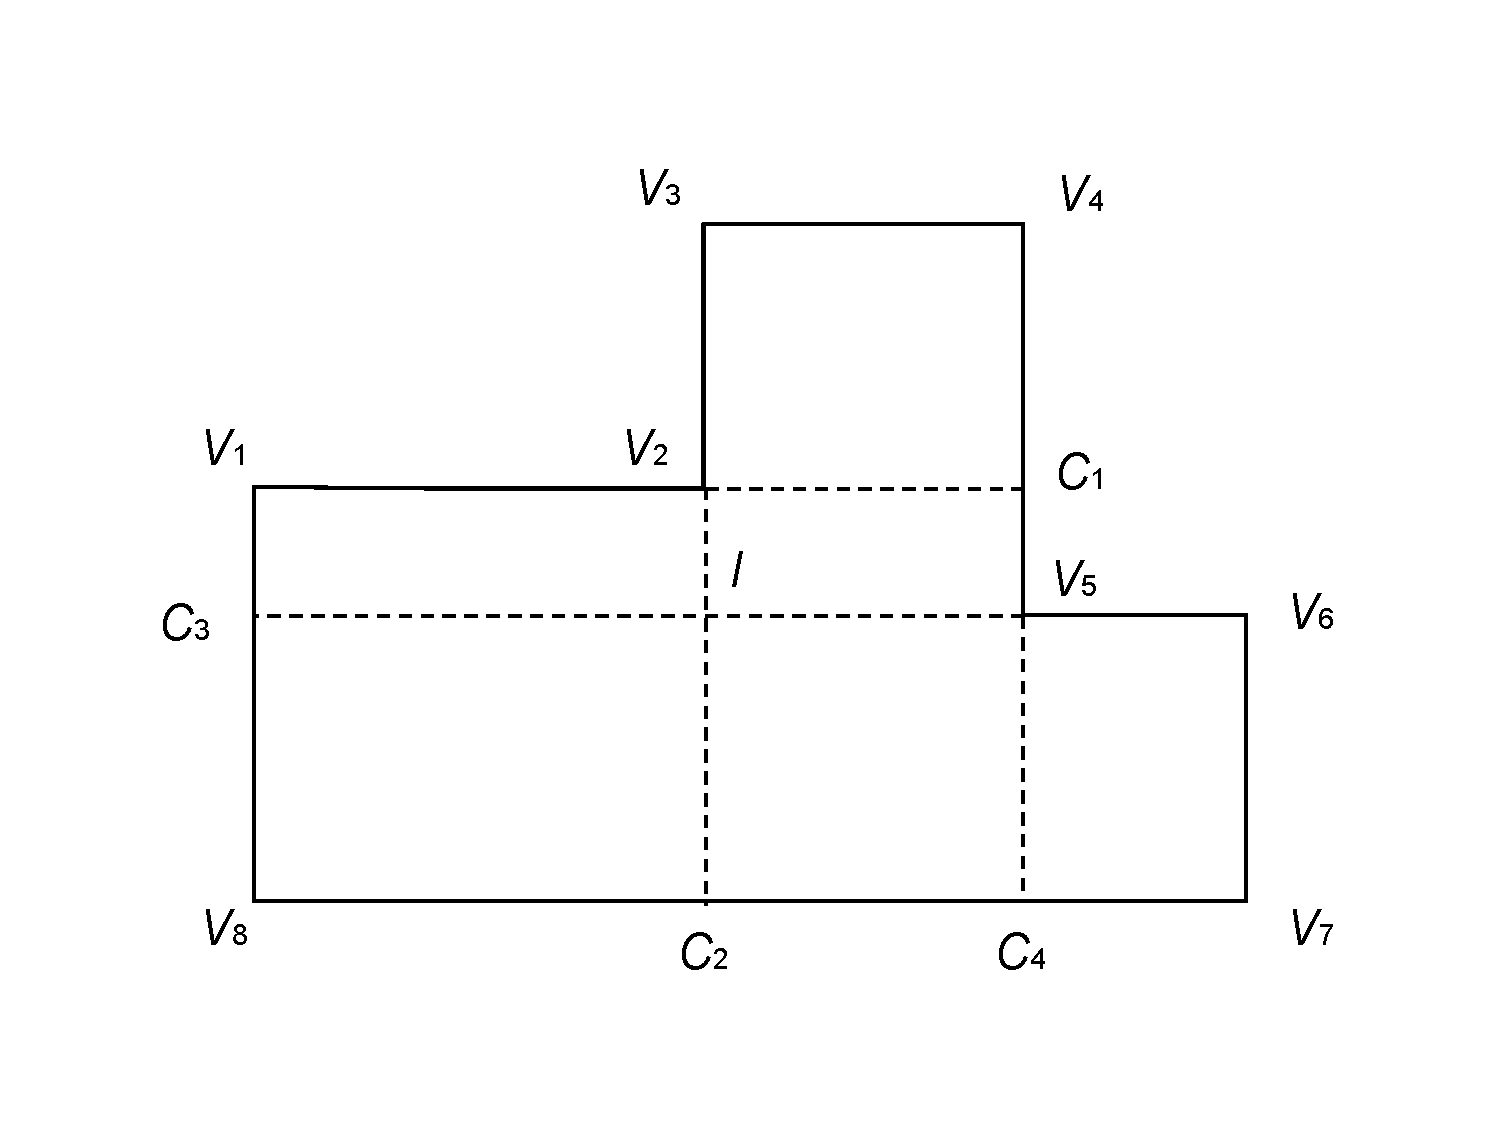
\includegraphics{./Pic/PDF/roofsegmentation/roofSegmentation.pdf}}}
			\\
		\end{tabular}}
		\caption{An example of input polygon vertices, cutting lines and six segmented components result.}
		\label{fig: roofsegment}
\end{figure} 

A detailed example is shown in Figure \ref{fig: roofsegment}, with input footprint vertices $V$. The first loop in algorithm can figure out $\{V_2, C_1\}$, $\{V_2, C_2\}$, $\{V_5, C_3\}$ and $\{V_5, C_4\}$ are cutting lines. The first cut to $V$ by $\{V_2, C_1\}$ will get $\{V_2, V_3, V_4, V_5\}$ and $\{V_1, C_1, V_5, V_6, V_7, V_8\}$ these two polygons. Iterate all cutting lines until I get six segmented polygons. 

An example of roof segmentation using the proposed approach is given in Figure \ref{fig: segmentationexample} in which a building roof is divided to 7 pieces.

\begin{figure}[htb]
	\centerline{
		\begin{tabular}{cc}
			\resizebox{0.45\textwidth}{!}{\rotatebox{0}{
					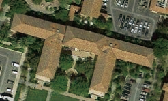
\includegraphics{./Pic/PDF/roofsegmentation/entire.pdf}}}
			&
			\resizebox{0.5\textwidth}{!}{\rotatebox{0}{
					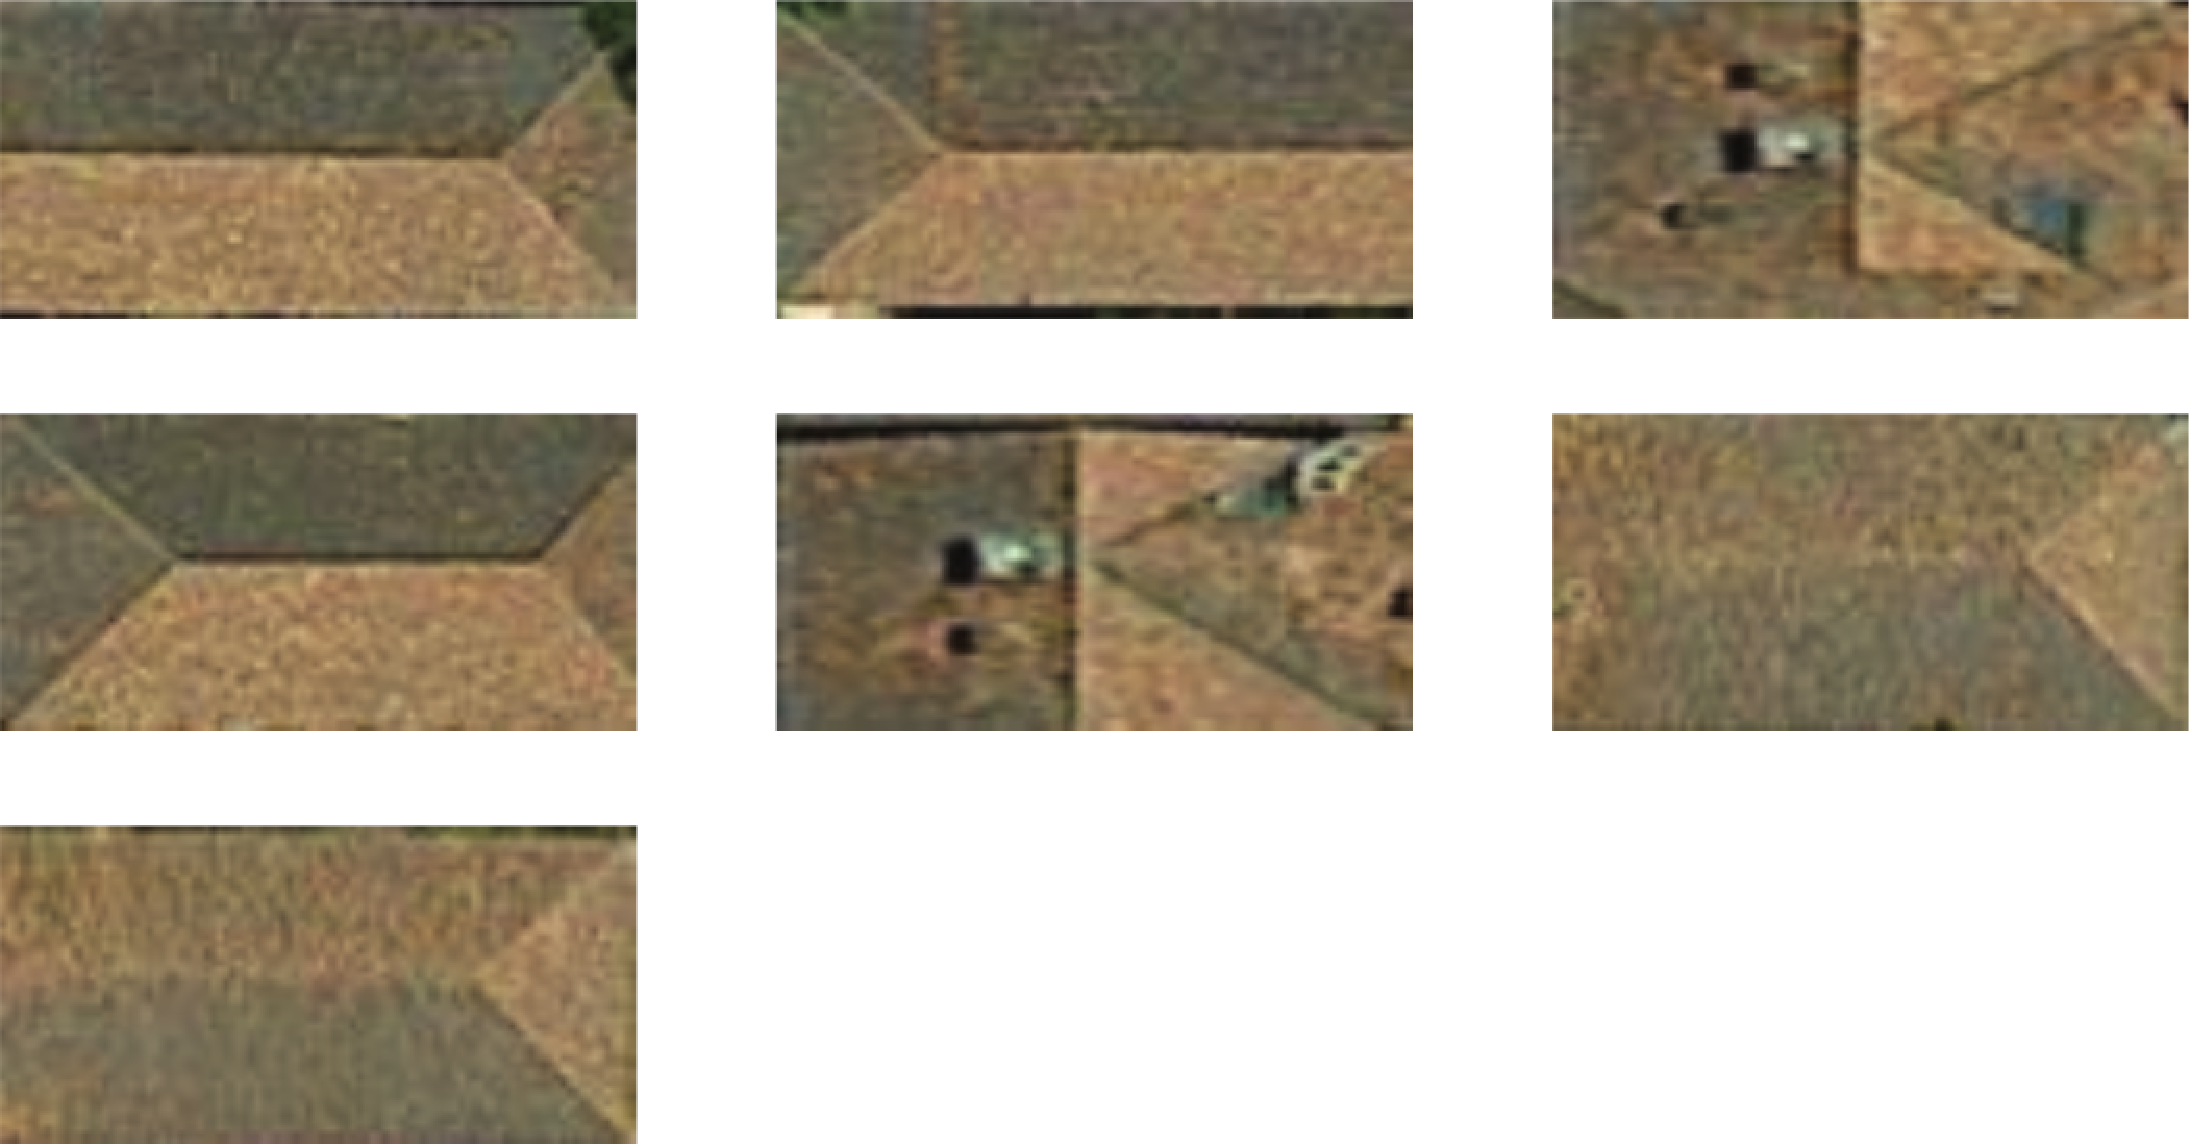
\includegraphics{./Pic/PDF/roofsegmentation/allpieces.pdf}}}
			\\
			(a) & (b)
		\end{tabular}}
		\caption{An example of segmentation on a complex building roof. All pieces are normalize to a same dimension.}
		\label{fig: segmentationexample}
\end{figure} 

Later all roof top images are aligned using an approach proposed in \cite{ZQY:08}. Then all images are resized to the same dimension. This dataset is of great challenges for the task of visual analysis. First, qualities of the some satellite images are degraded because of significant image blurring occurred when capturing the satellite images. Second, roofs in these images are covered by various kinds of equipments such as air conditioners chimneys and water tanks, and most of roofs in my dataset are partially occluded by shadows cast by trees and some other stuffs. Such covering and shadows are great obstacles to robust visual analysis algorithms. Examples of my data in this dataset is given in Figure \ref{fig: roofexamples}

\begin{figure}[htb]
	\centerline{
		\begin{tabular}{c}
			\resizebox{0.95\textwidth}{!}{\rotatebox{0}{
					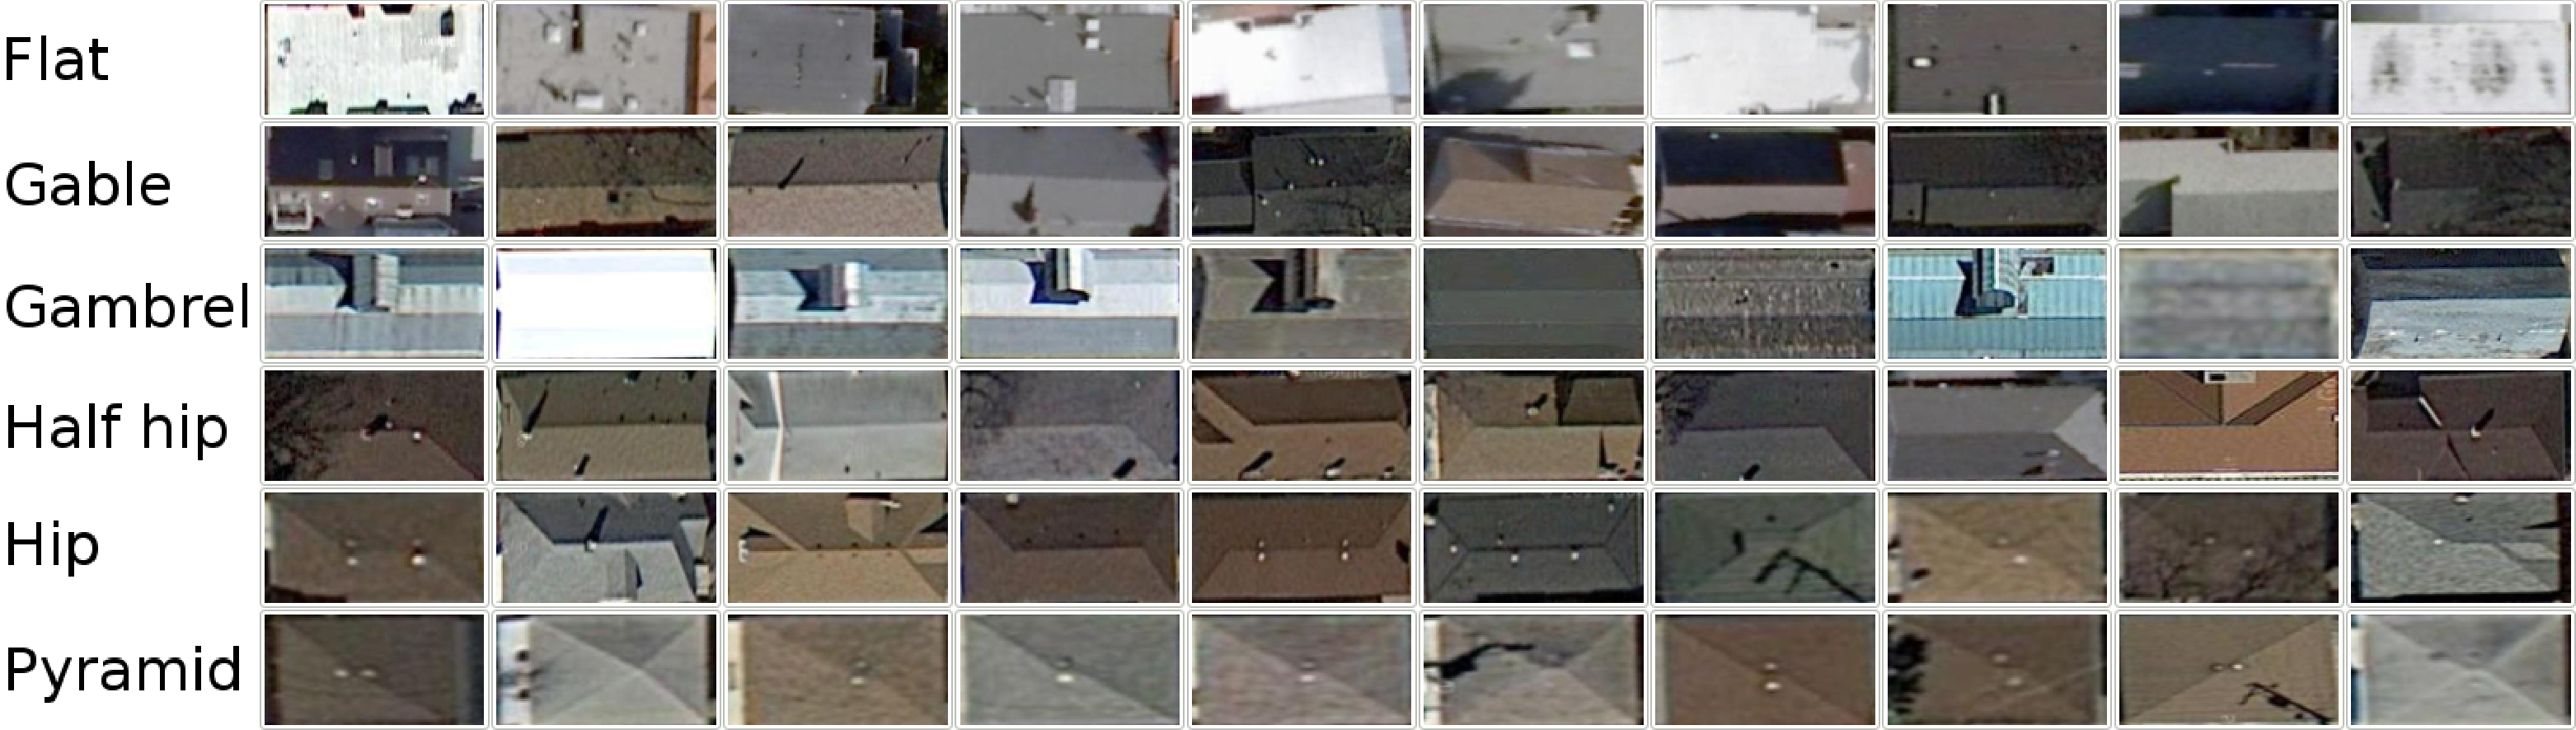
\includegraphics{./Pic/PDF/AllRoofsExamples.pdf}}}
		\end{tabular}}
		\caption{Examples of roof top images used in my work.}
		\label{fig: roofexamples}
\end{figure} 

Furthermore, the class instances of this dataset are intrinsically extremely unbalanced that some particular types of roofs (such as gambrel and pyramid) are far less than the other types. Such unbalanced distributions of data are compared in Table \ref{Tab: datadistribution}.

\begin{table}[h]
\protect\protect\caption{The distribution of the roof styles used in the experiments.}
\centering %
\begin{tabular}{lccc}
\hline\hline
Styles  & Training \#  & Testing \#  & Total \# \tabularnewline
\hline
Flat  & 1232  & 1748  & 3080 \tabularnewline
Gable  & 1111  & 1665  & 2776 \tabularnewline
Gambrel  & 156  & 232  & 388 \tabularnewline
Halfhip  & 268  & 400  & 668 \tabularnewline
Hip  & 960  & 1440  & 2400 \tabularnewline
Pyramid  & 133  & 199  & 332 \tabularnewline
\hline
\end{tabular}
\label{Tab: datadistribution} 
\end{table}

Classification of the roof styles in the experiments are based on recognizing edges detected from the roof images. I employed the adaptive Otsu edge detection method \cite{otsu:79} to extract edges from the roof images. Examples of generated edge images are shown in \ref{fig: roof edge demonstration}
(a). The synthetic prototypes are then created to characterize primary structures of a roof represented by extracted edges. The way I create synthetic models is to simplify and convert roof edge images to a parametric model in which edges are connected by a few control points. By adjusting the position of the control points and drawing lines between the points, I are able to simulate different variations of roof edge images. All noises and line patterns introduced by actual roof edge images are ignored in synthetic images, which makes it easier to create synthetic images. However, without present these noises and patterns in synthetic images potentially increase the distance between actual data and synthetic data, thus lower the accuracy of classifier trained using synthetic data. I will talk about techniques and algorithms dealing with these issues in Chapter \ref{chapter: learning from synthetic data} and Chapter \ref{chapter: synthetic gap} 

For all kinds of roof styles except flat I classified in my work, I intuitively design the parametric models of these roof edge images as the ones shown in Figure \ref{fig: controlpoints}.

\begin{figure}[h]
	\centerline{
		\begin{tabular}{ccccc}
			\resizebox{0.18\textwidth}{!}{\rotatebox{0}{
					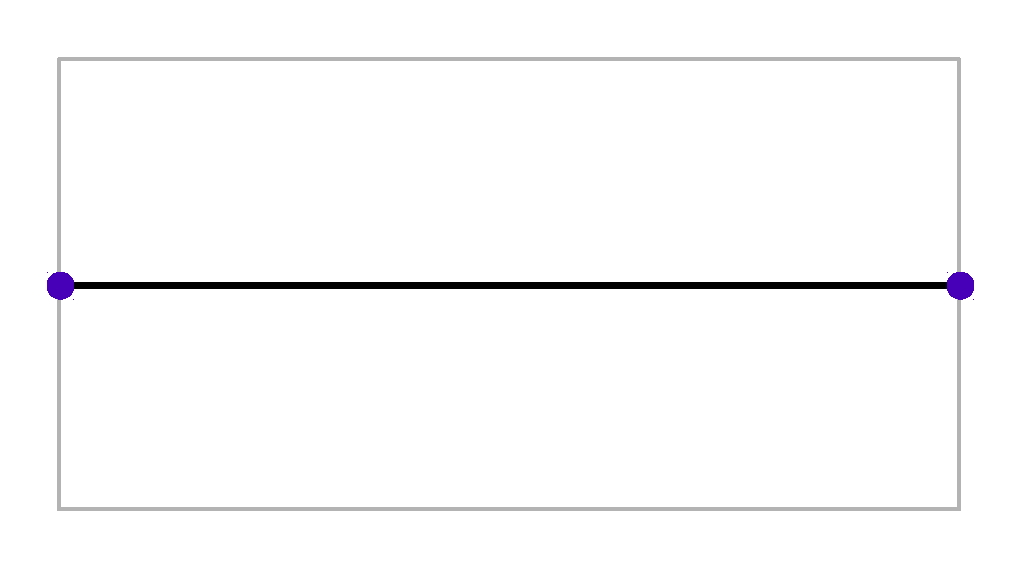
\includegraphics{./Pic/PDF/CoordinateDescentRange/Gable.pdf}}}
					&
			\resizebox{0.18\textwidth}{!}{\rotatebox{0}{
					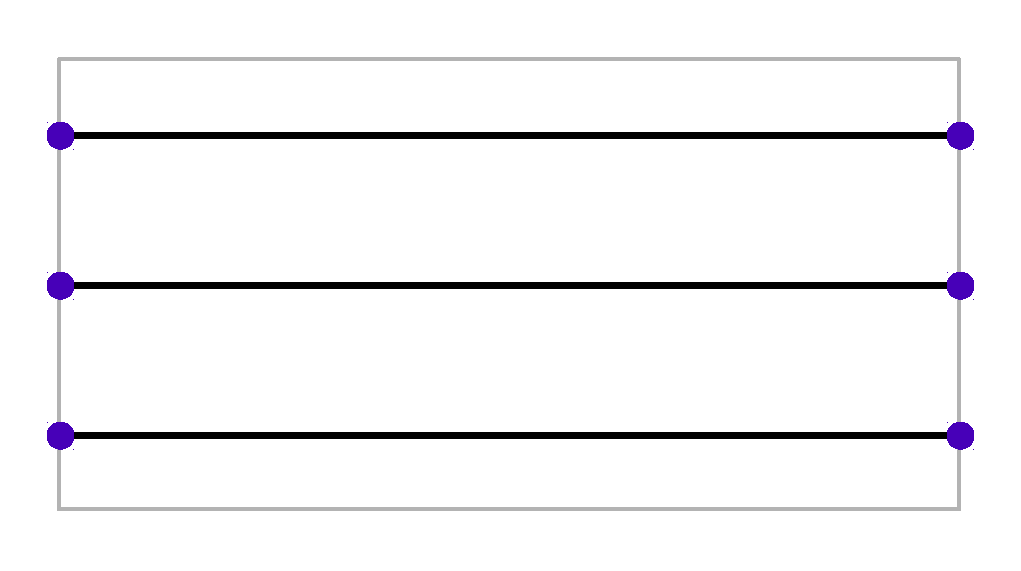
\includegraphics{./Pic/PDF/CoordinateDescentRange/Gambrel.pdf}}}
					&
			\resizebox{0.18\textwidth}{!}{\rotatebox{0}{
					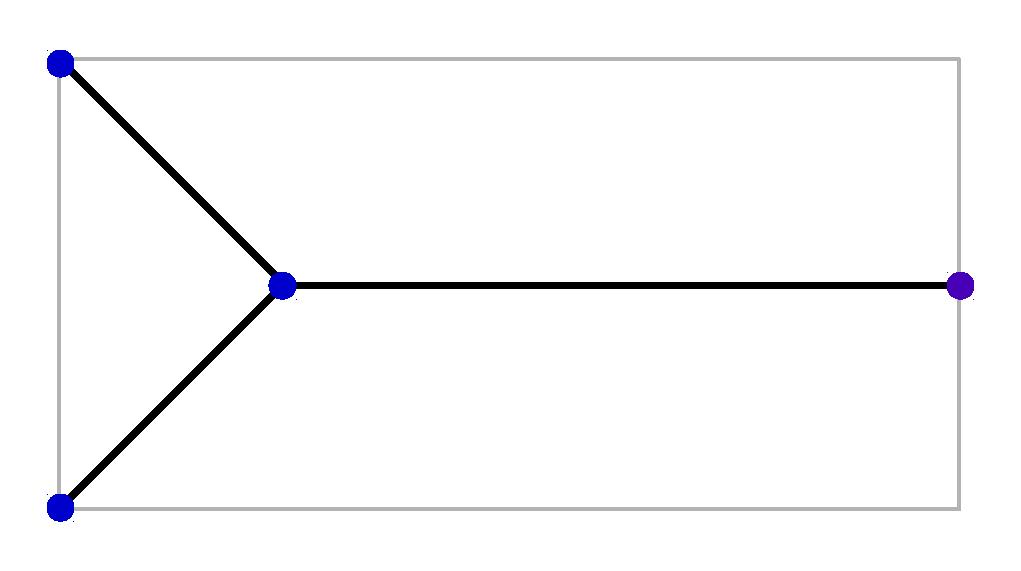
\includegraphics{./Pic/PDF/CoordinateDescentRange/Halfhip.pdf}}}
					&
			\resizebox{0.18\textwidth}{!}{\rotatebox{0}{
					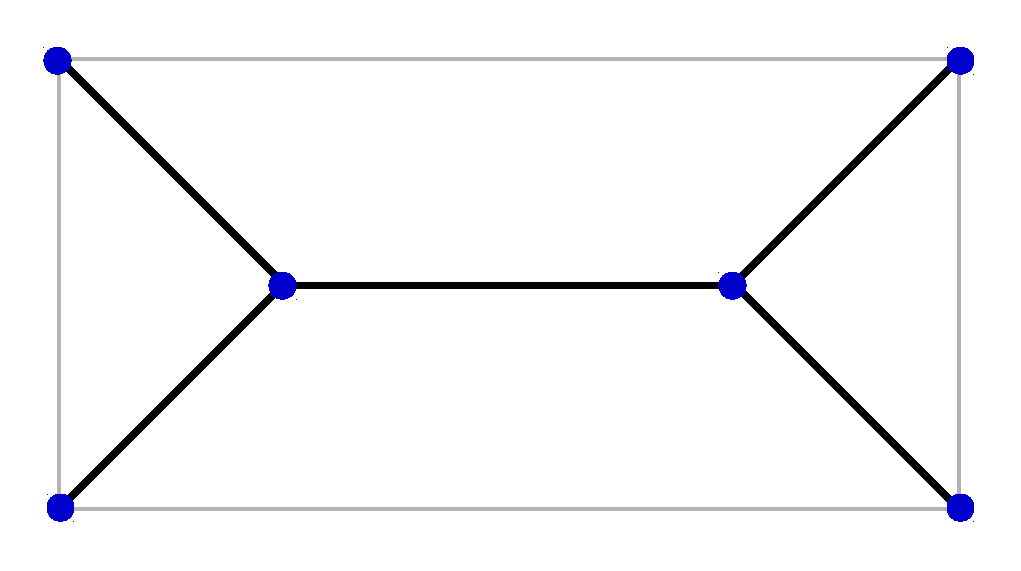
\includegraphics{./Pic/PDF/CoordinateDescentRange/Hip.pdf}}}
					&
			\resizebox{0.18\textwidth}{!}{\rotatebox{0}{
					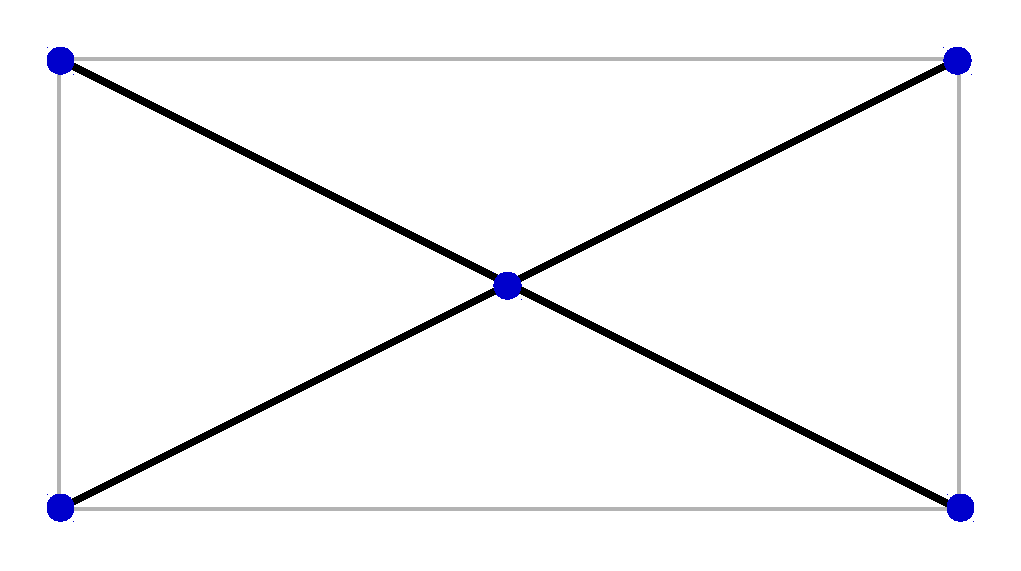
\includegraphics{./Pic/PDF/CoordinateDescentRange/Pyramid.pdf}}}		
					\\
			Gable & Gambrel & Halfhip & Hip & Pyramid \\
		\end{tabular}}
		\caption{For five roof styles used in my work, control points of each style are given in above figures which are shown as blue dots.}
		\label{fig: controlpoints}
\end{figure} 

With these basic synthetic template, generate more synthetic data is as easy as change positions of the control points. However, configuring these control points with arbitrary ranges will easily lead to a roof image that is impossible exist in real world thus introduce noises and outliers to dataset. To solve these problems, two approaches are proposed in my work \cite{Zhang2014Autoencoder} and \cite{ZX:14} separately.

In \cite{ZX:14}, I assume the position of each control points in image follows a normal distribution
that the set of control points: $\textbf{P}=\{p_i\}_{i=1}^k,\, p_i\, \sim\, N(\mu_i, \sigma_i) $. Thus for all control points $\textbf{P}$ of a roof style, they follow a multi-variant normal distribution that $\textbf{P}\, \sim\, N(\mu, \Sigma)$ where $\Sigma$ is covariance matrix of $\textbf{P}$. To estimate parameters mean and covariance of existing data set, volunteers are invited to help us mark the control points of actual data. Then $\mu$ and $\Sigma$ are computed from the marked point positions. To illustrate distribution of each control points in my roof edge templates, I rendered points' distribution in Figure \ref{fig: controlpointsdistribution}. At this point, control points of a synthetic data could be randomly drawn from multivariate normal distribution $N(\mu, \Sigma)$ I just computed. 

\begin{figure}[h]
	\centerline{
		\begin{tabular}{ccccc}
			\resizebox{0.18\textwidth}{!}{\rotatebox{0}{
					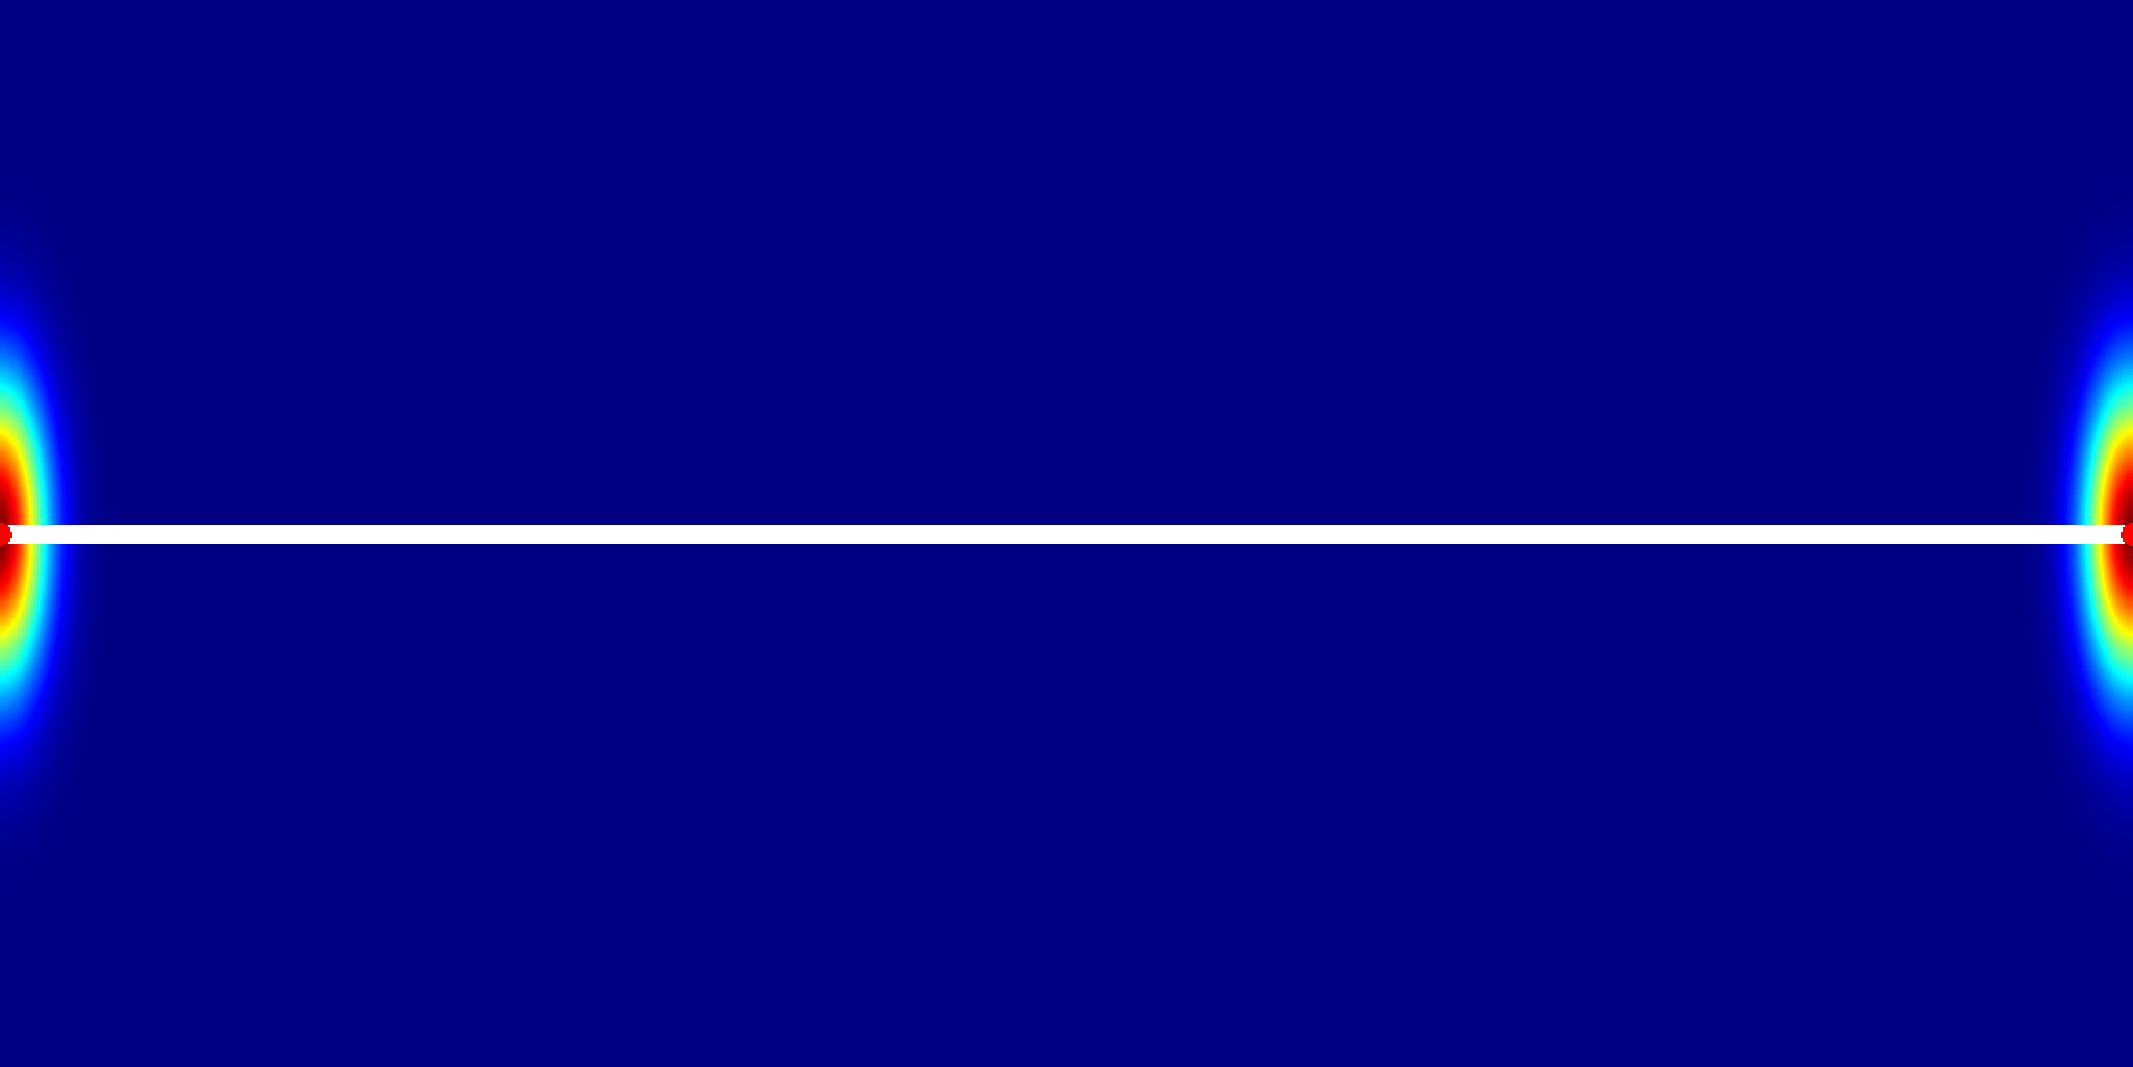
\includegraphics{./Pic/PDF/roofkeypointdistribution/withedgedots/gable.pdf}}}
					&
			\resizebox{0.18\textwidth}{!}{\rotatebox{0}{
					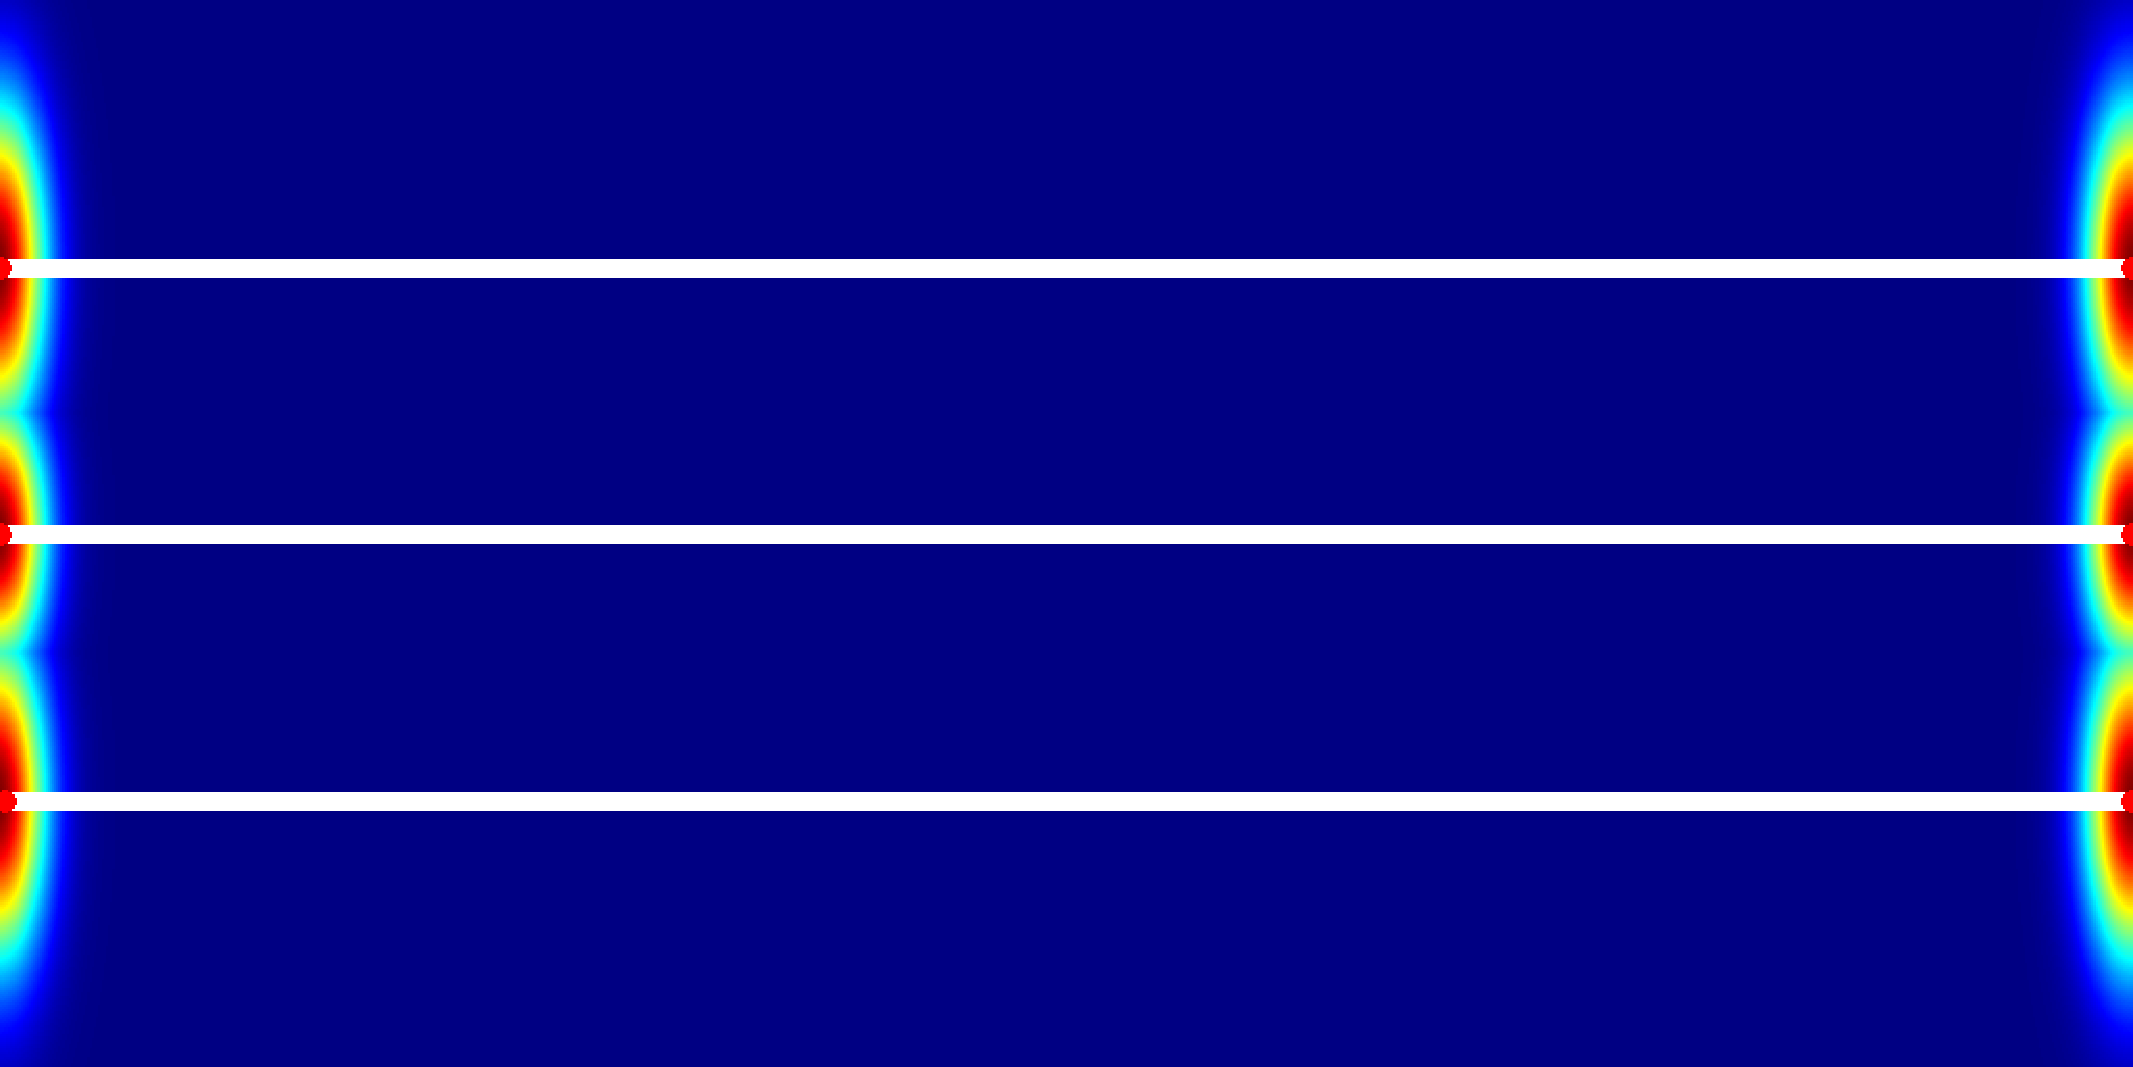
\includegraphics{./Pic/PDF/roofkeypointdistribution/withedgedots/gambrel.pdf}}}
					&
			\resizebox{0.18\textwidth}{!}{\rotatebox{0}{
					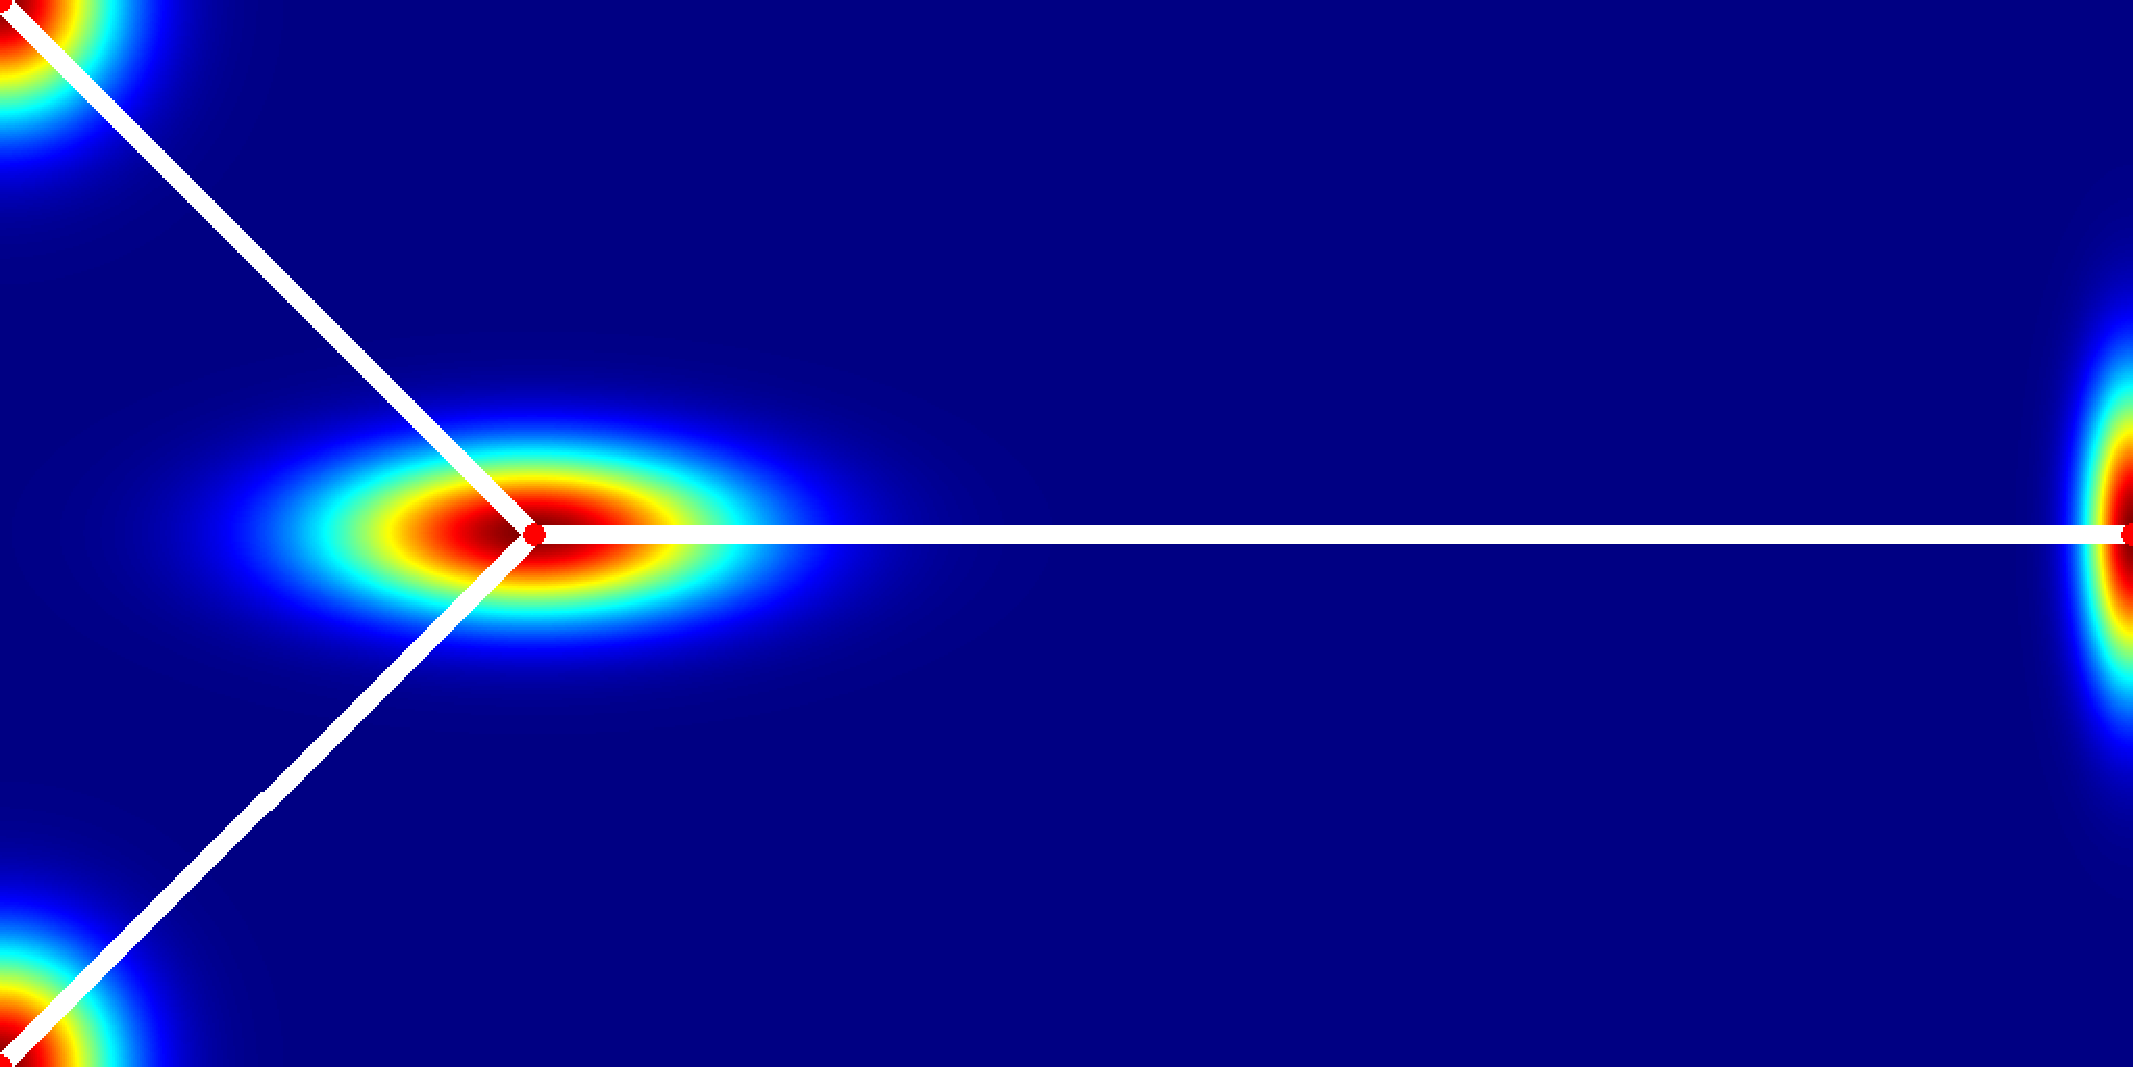
\includegraphics{./Pic/PDF/roofkeypointdistribution/withedgedots/halfhip.pdf}}}
					&
			\resizebox{0.18\textwidth}{!}{\rotatebox{0}{
					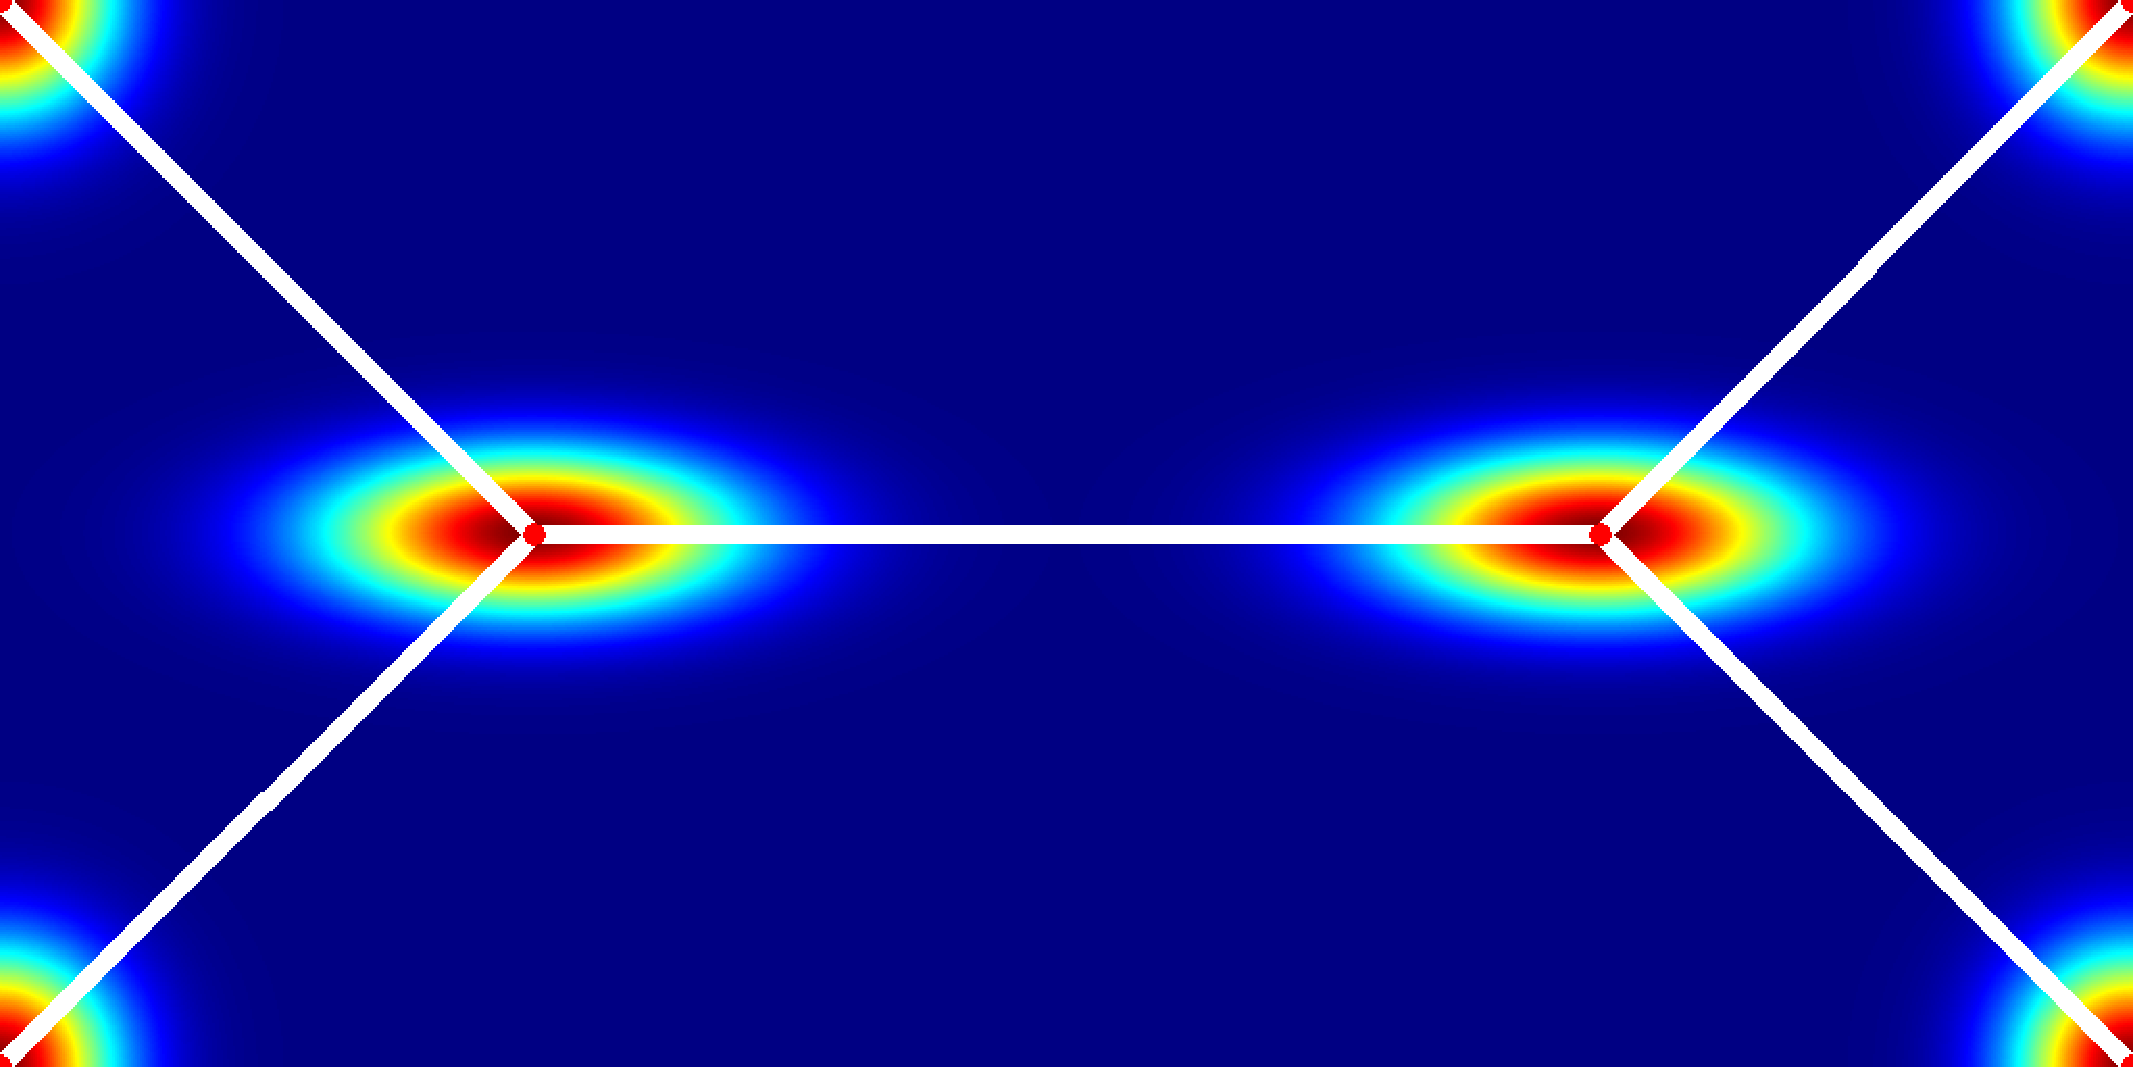
\includegraphics{./Pic/PDF/roofkeypointdistribution/withedgedots/hip.pdf}}}
					&
			\resizebox{0.18\textwidth}{!}{\rotatebox{0}{
					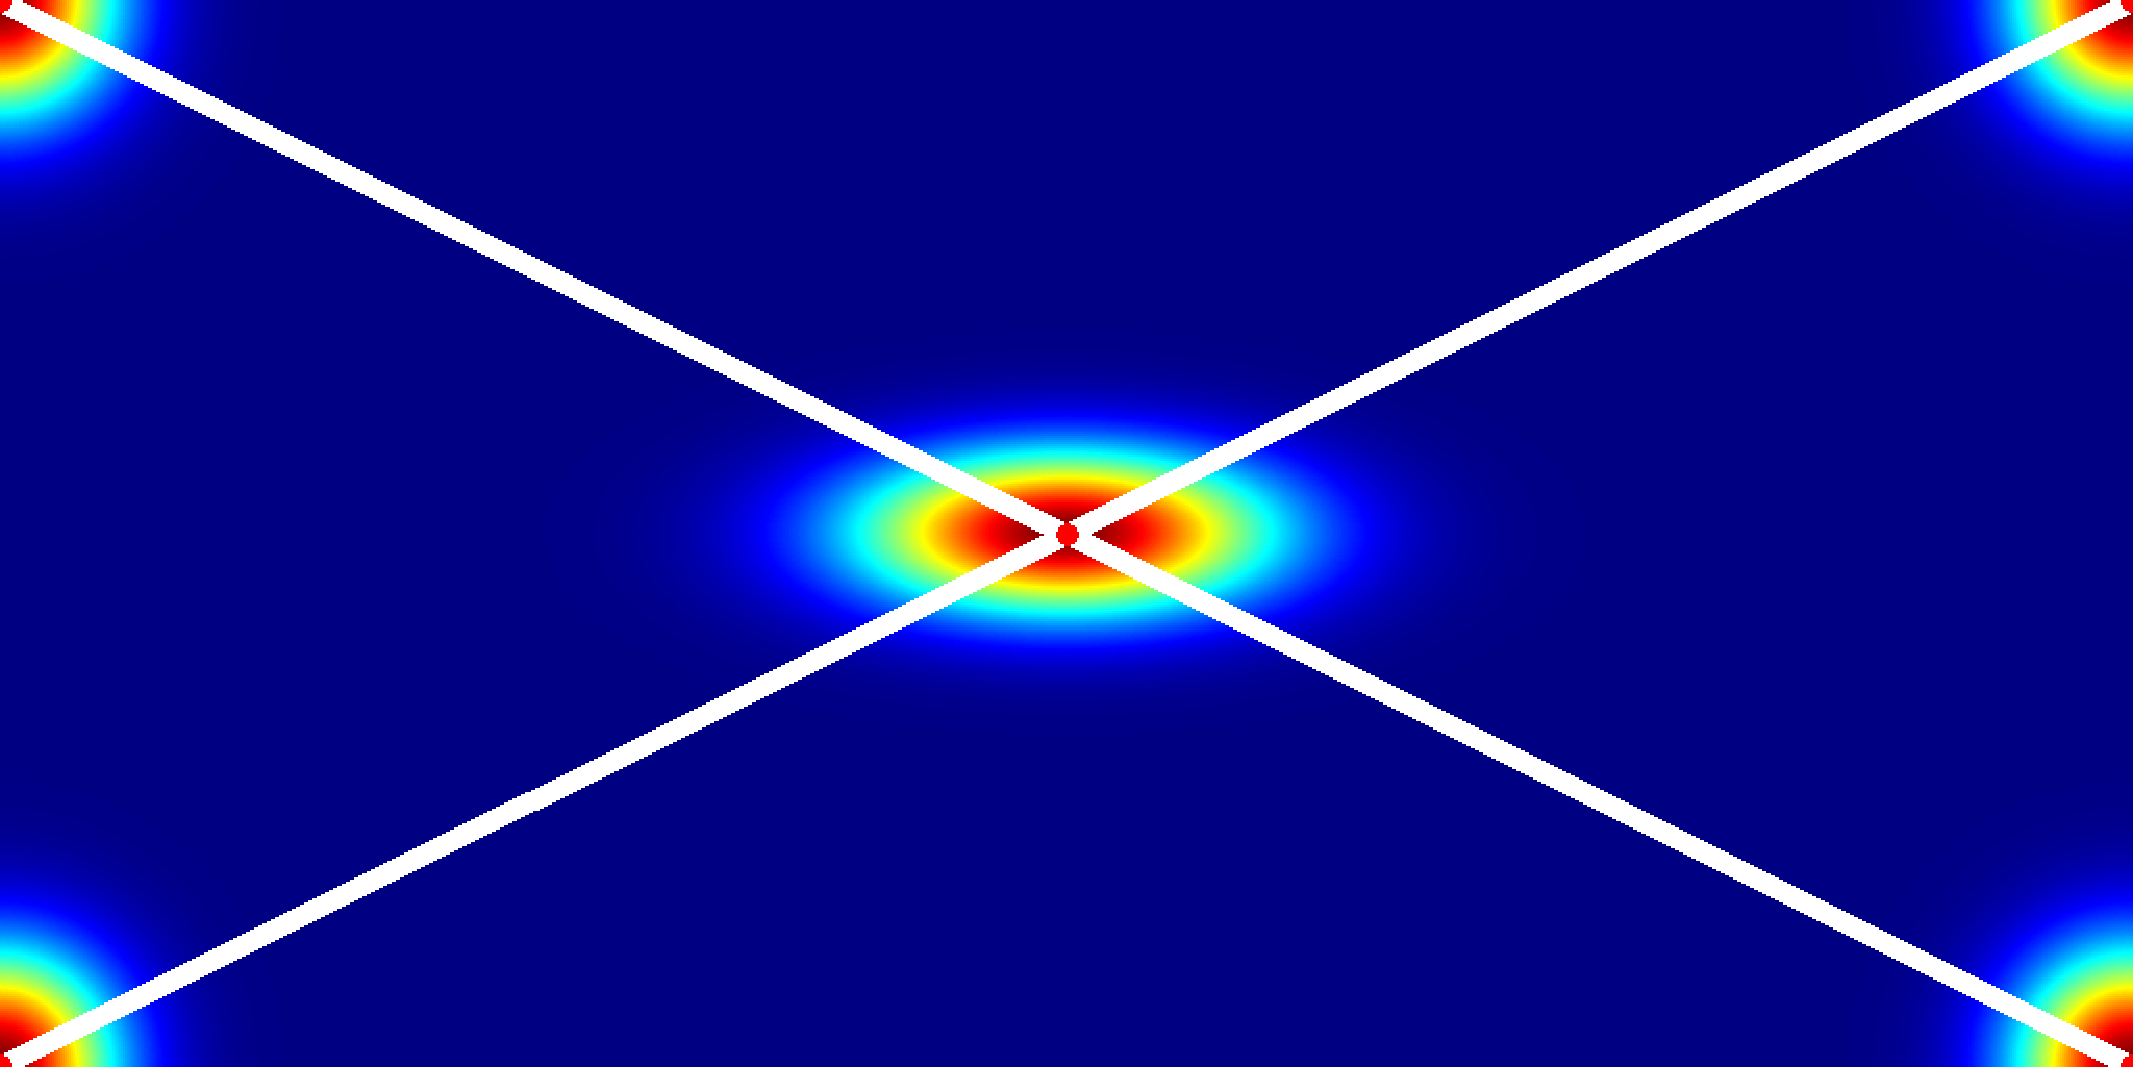
\includegraphics{./Pic/PDF/roofkeypointdistribution/withedgedots/pyramid.pdf}}}		
					\\
			Gable & Gambrel & Halfhip & Hip & Pyramid \\
		\end{tabular}}
		\caption{For five roof styles used in my work, control points of each style are given in above figures which are shown as blue dots.}
		\label{fig: controlpointsdistribution}
\end{figure} 

There are several disadvantages in above approach by inviting volunteer to do the labelling and assuming underlining distribution of control points. First, manually marking control points is an annoying task that it is time consuming and easy to make mistakes. Second, assuming underlying distribution of the control points is multivariate normal distribution may be problematic, especially when the number of samples is small, such as gambrel and pyramid roof styles in my work.  

So, in \cite{Zhang2014Autoencoder}, I propose a different method to obtain positions of the control points and construct synthetic data. In \cite{Zhang2014Autoencoder}, the synthetic data are represented as a parametric model of a set of control points and edges associated to these points in the images. From the control points, the synthetic
images could be generated to simulate the real images in terms of having the same structure or a similar appearance. Initially, the control points are selected from a synthetic prototype that generalize all images in the same class. Then the locations of the control points are iteratively optimized until convergence in order to minimize the distance between synthetic images generated by control points and the real image. I annotate the control points and edges associated to them as $\textbf{S}=\{\textbf{P},\textbf{E}\}$, where $\textbf{P}=\{p_{i}\}_{i=1}^{n}$ is the set of the control points, and $\textbf{E}=\{(p_{i},p_{j})\},1\leq i,j\leq n$ is the set of edges connecting control points. A generalized algorithm of getting the best matching synthetic image is provided in Algorithm \ref{Alg: MatchingSynthetic}.

{\linespread{1.5}
\begin{algorithm}[htb]  
\small
 	\caption{ Get Matching Synthetic Image.}   
	\label{Alg: MatchingSynthetic}    	
\begin{algorithmic}[1]  	\REQUIRE ~~\\ 		
$\bullet$ A real image $U$. \\ 	
	$\bullet$ A set of control points 
$\textbf{S}=\{\textbf{P}, \textbf{E}\}$ 
with all control points $p_i\in \textbf{P}$ set to their initial positions.\\ 	
	$\bullet$ A prototype image $V$ generated using the initial $\textbf{S}$.  \\ 	
	\WHILE{\textbf{S} is not converged} 	
		\STATE \textbf{S} = OptimizeControlPoints($U, V, \textbf{S}$). 		
	\STATE Generate $V$ using $\textbf{S}$. 		
\ENDWHILE 
		\STATE Generate synthetic image $I$ using \textbf{S}. 	
	\RETURN $I$. 	
\end{algorithmic} 
 \end{algorithm}  
}

In Algorithm \ref{Alg: MatchingSynthetic}, the OptimizeControlPoints(U, V, \textbf{S}) function is a process that searches for optimal control point locations which results in a synthetic image minimizing the discrepancy between the real image and the synthetic image. A coordinate descent framework is employed to accelerate the search process. I summarize this method in Algorithm \ref{Alg: OCP1}.

{\linespread{1.5}
\begin{algorithm}[htb]  
\small
 	\caption{ OptimizeControlPoints($U, V, \textbf{S}$) Case 1}   
	\label{Alg: OCP1}    
	\begin{algorithmic}[1]  		\REQUIRE ~~\\ 
		$\bullet$ A real image $U$. \\ 
		$\bullet$ A prototype of the synthetic image $\textbf{S}=\{\textbf{P}, \textbf{E}\}$.\\ 	
	$\bullet$ A synthetic image $V$ generated using $\textbf{S}$.  \\ 	
	\FOR{$p_i\in \textbf{P}, 1\leq i \leq n$} 		\STATE Update $\textbf{S}$ by moving $p_i$ by one unit. 	
	\STATE Generate $V$ using \textbf{S}. 	
	\IF {$\textbf{S}$ does not reduce Dist($U, V$)} 
			\STATE Cancel the last move of $p_i$. 	
		\STATE Generate $V$ using \textbf{S}. 	
	\ENDIF 	
	\ENDFOR 	
	\RETURN \textbf{S}. 	
\end{algorithmic}   
\end{algorithm}  
}

As I mentioned previously, make an assumption that the underlying distribution of control points is multivariate normal distribution may not be appropriate in some cases, especially for a case where only a few samples are given in a high dimensional space. So, I propose another technique which does not make any assumption about the distribution of the control points, thus no parameter need to be estimated if using this method. 

{\linespread{1.5}
\begin{algorithm}[htb]  
\small
 	\caption{ RNNI($I, k, N$)}   
	\label{Alg: RNNI}    
	\begin{algorithmic}[1]  		
	\REQUIRE ~~\\ 
		$\bullet$ Set of input images that are to be interpolated $I=\{\textbf{S}_i\}_{i=1}^n$. \\ 
		$\bullet$ The number of nearest neighbors $k$. \\ 	
		$\bullet$ The number synthetic data to be generated $N$. \\
	\ENSURE ~~\\
		$\bullet$ Set of generated synthetic data $I$. 	
	\FOR{ $1\leq i \leq N$} 		
	\STATE Randomly choose a integer number $idx$ that $1\leq idx \leq n$. 	
	\STATE Randomly choose a neighbor from k nearest neighbor of $\textbf{S}_{idx}$ and call it $\textbf{S}_j$.
	\STATE Randomly choose a floating number r that $0\leq r \leq 1$.	
	\STATE $\textbf{P}_{new}=\textbf{P}_{idx}+r\times(\textbf{P}_j-\textbf{P}_{idx})$.
	\STATE Connect $\textbf{P}_{new}$ in a proper way to draw roof edges $\textbf{E}_{new}$.
	\STATE $\textbf{S}_{new}=\{\textbf{P}_{new}, \textbf{E}_{new}\}$.
	\STATE $\textbf{I}=\textbf{I}\cup \textbf{S}_{new}$.
	\ENDFOR 	
	\RETURN \textbf{I}. 	
\end{algorithmic}   
\end{algorithm}  
}

The synthetic data generated in this approach is based on interpolation between a sample data and one of its nearest neighbors. The interpolation is done on each existing sample. I call this method as Random Nearest Neighbors Interpolation (RNNI) to emphasize the randomness in the selection of nearest neighbor. Similar methods are used in a lot of previous works such as \cite{Comput.Sci.&Appl.Math.1997}, where to facilitate character recognize, interpolation is conducted on parameters of transformation such as skew, scale and so on. my method is different from previous works that instead of compute underlying transformation, for the sake of using control points the interpolation in my approach is directly applied on data itself which makes the entire procedure easier and effective. The algorithm that generate a set of new synthetic data is given in Algorithm \ref{Alg: RNNI}.

\Subsection{Hand Written Digital Character Recognition} Synthetic data is helpful in a lot of applications, another example that benefit from my method is hand written digital character recognition. I also validate my framework on handwritten digits dataset from
UCI machine learning repository \cite{Bache+Lichman:2013} which totally has $5620$ instances. The handwritten digits from $0$ to $9$ in this dataset are collected from $43$ people: $30$ contributed to the training set and the other $13$ to the test set. 

Generation of synthetic data in hand written digital character dataset is still done by interpolation using Algorithm \ref{Alg: RNNI}. However, different from roof edge images, hand written digit is much more complicated, manually marking control points is almost impossible. Due to complexity of the digit character, dozens of control points must be used to guarantee the quality of synthetic digital character. Under such high dimension space of control points, it makes it hopeless and inefficient to optimize control points using approach such as Algorithm \ref{Alg: OCP1}. Therefore, I adopt a different strategy and using an extra step to help constructing the correspondence between control points of two digital images. 

To enable a interpolation with a better quality, a procedure called control point migration is adopted in my work to pair up control points of different images. The idea of the approach is to first compute an root image for all images with the same digit character which summarizes the digit character in all images. Then on this root image I could set up some control points which later could be migrated to all other images. Since for all images control points are   from the same root image, their are already paired up. 

A method called congealing proposed in \cite{ME:00} is adopted here to generate root images. In congealing, the project transformations are applied to images to minimize a joint entropy. Thus the root image actually can be considered as an average image of all images after congealing. I show all the root images in Figure \ref{fig: rootimage}.

\begin{figure}[h]
	\centerline{
		\begin{tabular}{ccccc}
			\resizebox{0.18\textwidth}{!}{\rotatebox{0}{
					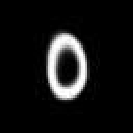
\includegraphics{./Pic/PDF/CongealDigits/mean_img0.pdf}}}
					&
			\resizebox{0.18\textwidth}{!}{\rotatebox{0}{
					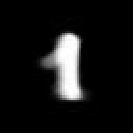
\includegraphics{./Pic/PDF/CongealDigits/mean_img1.pdf}}}
					&
			\resizebox{0.18\textwidth}{!}{\rotatebox{0}{
					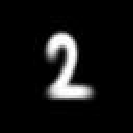
\includegraphics{./Pic/PDF/CongealDigits/mean_img2.pdf}}}
					&
			\resizebox{0.18\textwidth}{!}{\rotatebox{0}{
					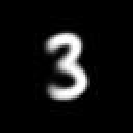
\includegraphics{./Pic/PDF/CongealDigits/mean_img3.pdf}}}
					&
			\resizebox{0.18\textwidth}{!}{\rotatebox{0}{
					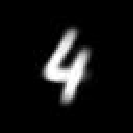
\includegraphics{./Pic/PDF/CongealDigits/mean_img4.pdf}}}		
					\\ \\
			\resizebox{0.18\textwidth}{!}{\rotatebox{0}{
					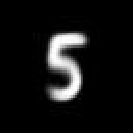
\includegraphics{./Pic/PDF/CongealDigits/mean_img5.pdf}}}
					&
			\resizebox{0.18\textwidth}{!}{\rotatebox{0}{
					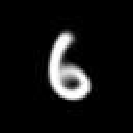
\includegraphics{./Pic/PDF/CongealDigits/mean_img6.pdf}}}
					&
			\resizebox{0.18\textwidth}{!}{\rotatebox{0}{
					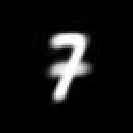
\includegraphics{./Pic/PDF/CongealDigits/mean_img7.pdf}}}
					&
			\resizebox{0.18\textwidth}{!}{\rotatebox{0}{
					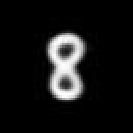
\includegraphics{./Pic/PDF/CongealDigits/mean_img8.pdf}}}
					&
			\resizebox{0.18\textwidth}{!}{\rotatebox{0}{
					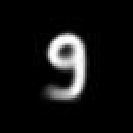
\includegraphics{./Pic/PDF/CongealDigits/mean_img9.pdf}}}	
		\end{tabular}}
		\caption{Root images of all kinds of digit characters.}
		\label{fig: rootimage}
\end{figure} 

Then control points are evenly sampled from the boundary detected from the prototype image. The control points needs to be mapped to each digit image in order to build correspondence with other images. To find this mapping I implement an approach that migrates the control points from the prototype images to destination image. Basically, given two sets of control points on two images, finding a matching between each pair of points is a bipartite matching problem, which may need some sort of features to be computed for each control points and could be solving using discrete optimization method. Additional constraint also has to be added to the solution such as matched point pairs has to keep their original order. Such constraints make the problem even harder to solve. In my method, however, the idea is very simple yet very effective that I slightly change source image a little bit towards the target image, and move the control points in the same time. my method achieve very good quality when intermediate steps are dense enough.

\begin{figure}[ht]
\centerline{ %
\begin{tabular}{ccccccc}
\resizebox{0.12\textwidth}{!}{\rotatebox{0}{ 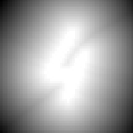
\includegraphics{./Pic/PDF/MigrateControlPoints/prototypeDT.pdf}}}  
& 
\resizebox{0.12\textwidth}{!}{\rotatebox{0}{ 
\includegraphics{./Pic/PDF/MigrateControlPoints/step1.pdf}}}  
& 
\resizebox{0.12\textwidth}{!}{\rotatebox{0}{ 
\includegraphics{./Pic/PDF/MigrateControlPoints/step2.pdf}}}  
& 
\resizebox{0.12\textwidth}{!}{\rotatebox{0}{ 
\includegraphics{./Pic/PDF/MigrateControlPoints/step3.pdf}}}  
& 
\resizebox{0.12\textwidth}{!}{\rotatebox{0}{ 
\includegraphics{./Pic/PDF/MigrateControlPoints/step4.pdf}}}  
& 
\resizebox{0.12\textwidth}{!}{\rotatebox{0}{ 
\includegraphics{./Pic/PDF/MigrateControlPoints/step5.pdf}}} 
& 
\resizebox{0.12\textwidth}{!}{\rotatebox{0}{ 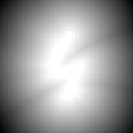
\includegraphics{./Pic/PDF/MigrateControlPoints/realDT.pdf}}} 
\end{tabular}} 
\caption{Illustrations of the migration of control points and intermediate
synthetic images generated using control points in each step. The
distance transform images of the synthetic prototype and real images
are shown as the left most and right most images respectively.}
\label{fig: migration1} 
\end{figure}

This point migration algorithm is based on a series of intermediate images generated in between synthetic prototype and destination image. To generate the intermediate images, I binarize all the images and the distance transformed images\cite{GB:86} of the synthetic prototype and the real image are generated. Given the number of steps, an intermediate image then is generated as a binarized image of linear interpolation between two distance transformed images. In each step, the control points are snapped to the closest boundary pixels of the intermediate image. The algorithm of OptimizeControlPoints($U,V,\textbf{S}$) in this situation is given in Algorithm \ref{Alg: OCP2}, I fix the number of steps to $10$ in this algorithm. The procedure of control points migration is shown in Figure \ref{fig: migration1} and Figure \ref{fig: migration2}. I recently notice that method proposed in \cite{lipovetsky2007efficient} is very similar to my migration approach.

{\linespread{1.5}
\begin{algorithm}[htb]    
\small
	\caption{ OptimizeControlPoints($U, V, \textbf{S}$) Case 2}  
 	\label{Alg: OCP2}    
	\begin{algorithmic}[1]  		\REQUIRE ~~\\ 	
	$\bullet$ A real image $U$. \\ 	
	$\bullet$ A prototype of the synthetic image $\textbf{S}=\{\textbf{P}, \textbf{E}\}$.\\ 	
	$\bullet$ A synthetic image $V$. 
\\ 	
	\STATE $steps=10$. 	
	\STATE Compute distance transform image of $U, V$ as $U', V'$. 	
	\FOR{$i=1$ to $steps$} 			
\STATE $I=(1-\frac{i}{steps})U'+\frac{i}{steps}V'$.\\
			\STATE $I$=Binarize($I$).\\ 	
		\STATE Update $\textbf{S}$ by snapping to the closest boundary pixel on $I$.\\ 	
	\ENDFOR 		\STATE Set the status of $\textbf{S}$ to be converged. 	
	\RETURN \textbf{S}. 	
\end{algorithmic} 
 \end{algorithm} 
}

\begin{figure}[ht]
\centerline{ %
\begin{tabular}{c}
\resizebox{0.3\textwidth}{!}{\rotatebox{0}{ 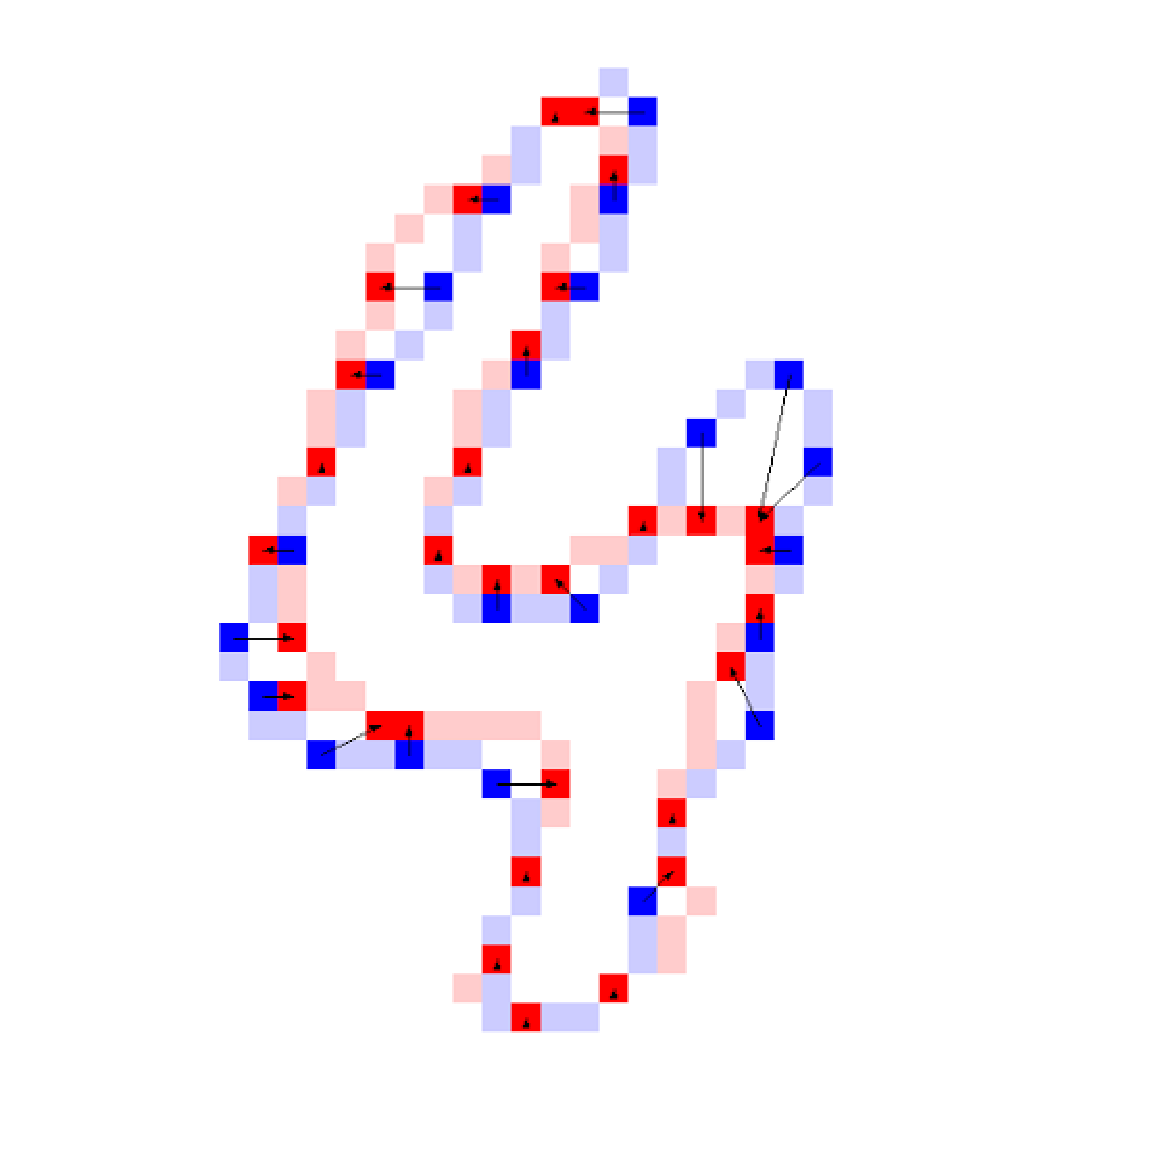
\includegraphics{./Pic/PDF/DigitReconstruction/move_4.pdf}}} 
\end{tabular}} 
\caption{Illustrations of the migration of control points for character 4. The control points are migrated from root image (blue) to destination image (red) and arrows are used to indicate points moving direction.}
\label{fig: migration2} 
\end{figure}

Once all images get their control points migrated from root image. More synthetic images could be generated using Algorithm \ref{Alg: RNNI}.

\Section{Creating Synthetic Data to Avoid Manual Labelling} 

One of requirement for a successful machine learning algorithm is abundant labelled data with high quality. Such dataset usually requires a long time and a lot of labor work to be done, which make the labelling work very expensive. In some cases, it is even impossible to finish labelling such as the problem of point cloud roof style recognition I solved in \cite{ZX:14}.

in \cite{ZX:14}, I proposed a learning based roof style classification algorithm using aerial LiDAR point clouds. The proposed approach is able to classify complex roof styles which may be composed of simple roof styles including: curve, flat, gable, hex, hip, mansard, pyramid, shed, gambrel, dome and unknown. All roof styles classified in my work are listed in 

\begin{figure}[ht]
\centerline{ %
\begin{tabular}{c}
\resizebox{0.6\textwidth}{!}{\rotatebox{0}{ 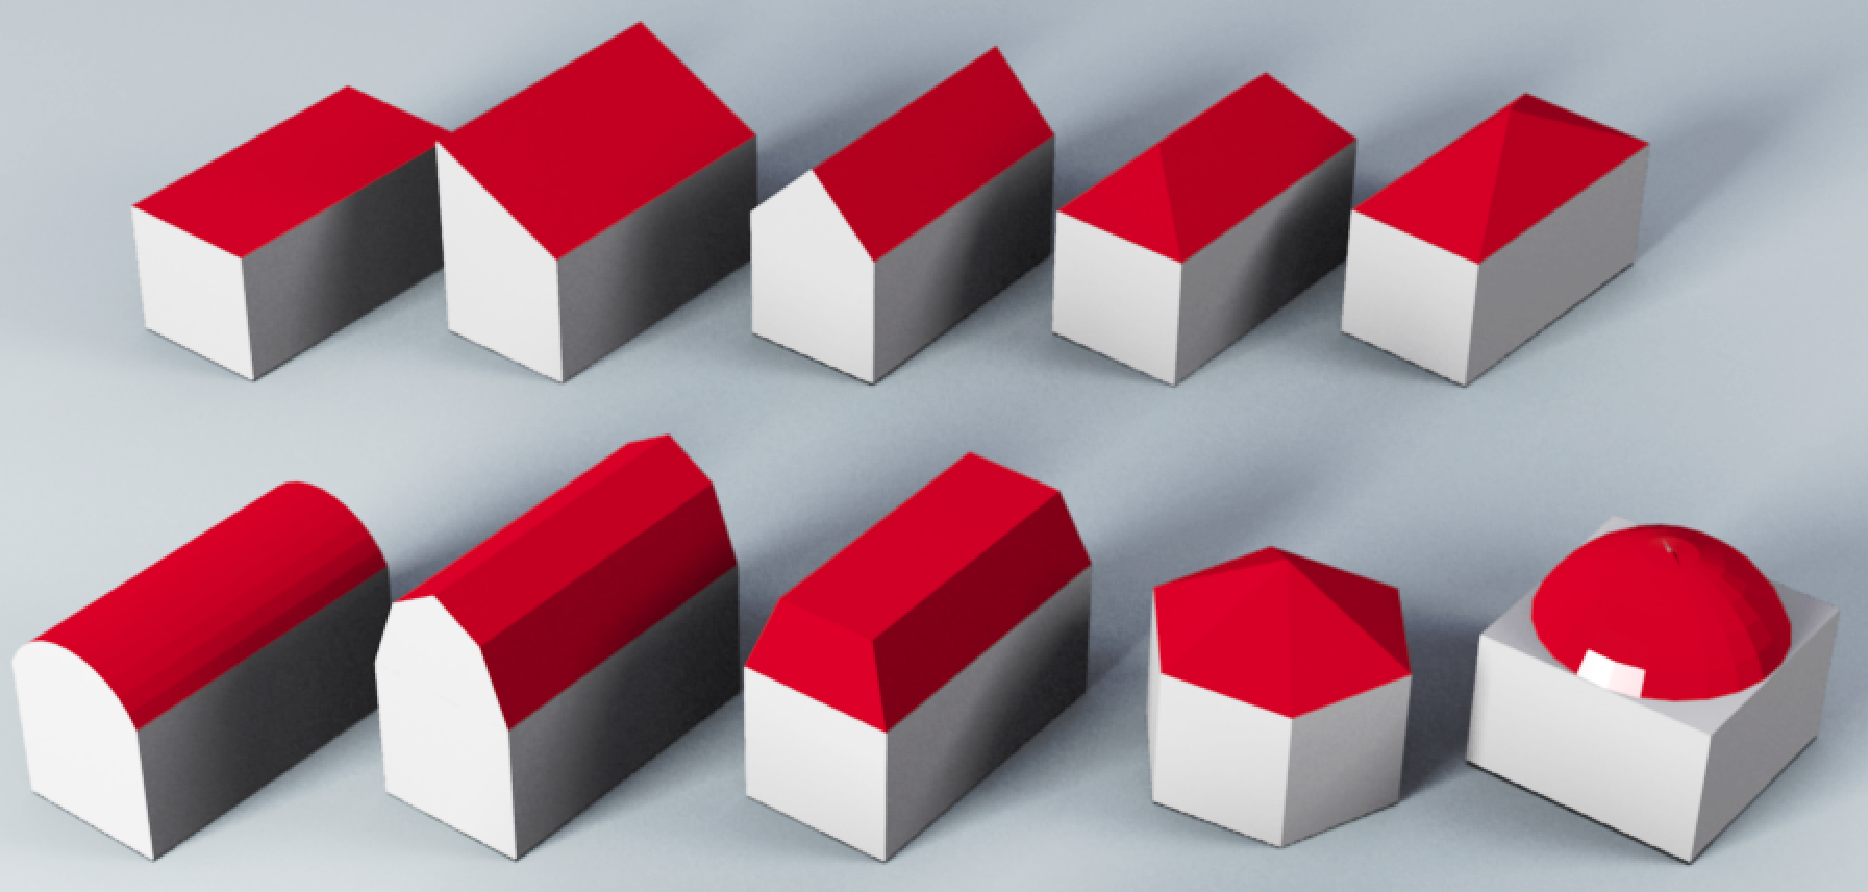
\includegraphics{./Pic/PDF/renderresultAllTypesTilt.pdf}}} 
\end{tabular}} 
\caption{Roof styles I classified in \cite{ZX:14}. From top to down, left to right: flat, shed, gable, hip, pyramid, curve, gambrel, mansard, hex and dome.}
\label{fig: allpointcloudroofstyles} 
\end{figure}

This method can easily accommodates more new roof styles by re-training of the new dataset with the new roof styles added. Because my method is implemented based on a bag of works schema. 

\begin{figure}[h]
\centerline{
\begin{tabular}{cccc}
  \resizebox{0.1\textwidth}{!}{\rotatebox{0}{
  
\includegraphics{Pic/PDF/BaseShape/Flat000.pdf}}}
  &
  \resizebox{0.20\textwidth}{!}{\rotatebox{0}{
  
\includegraphics{Pic/PDF/BaseShape/Gable000.pdf}}}
  &
  \resizebox{0.20\textwidth}{!}{\rotatebox{0}{
  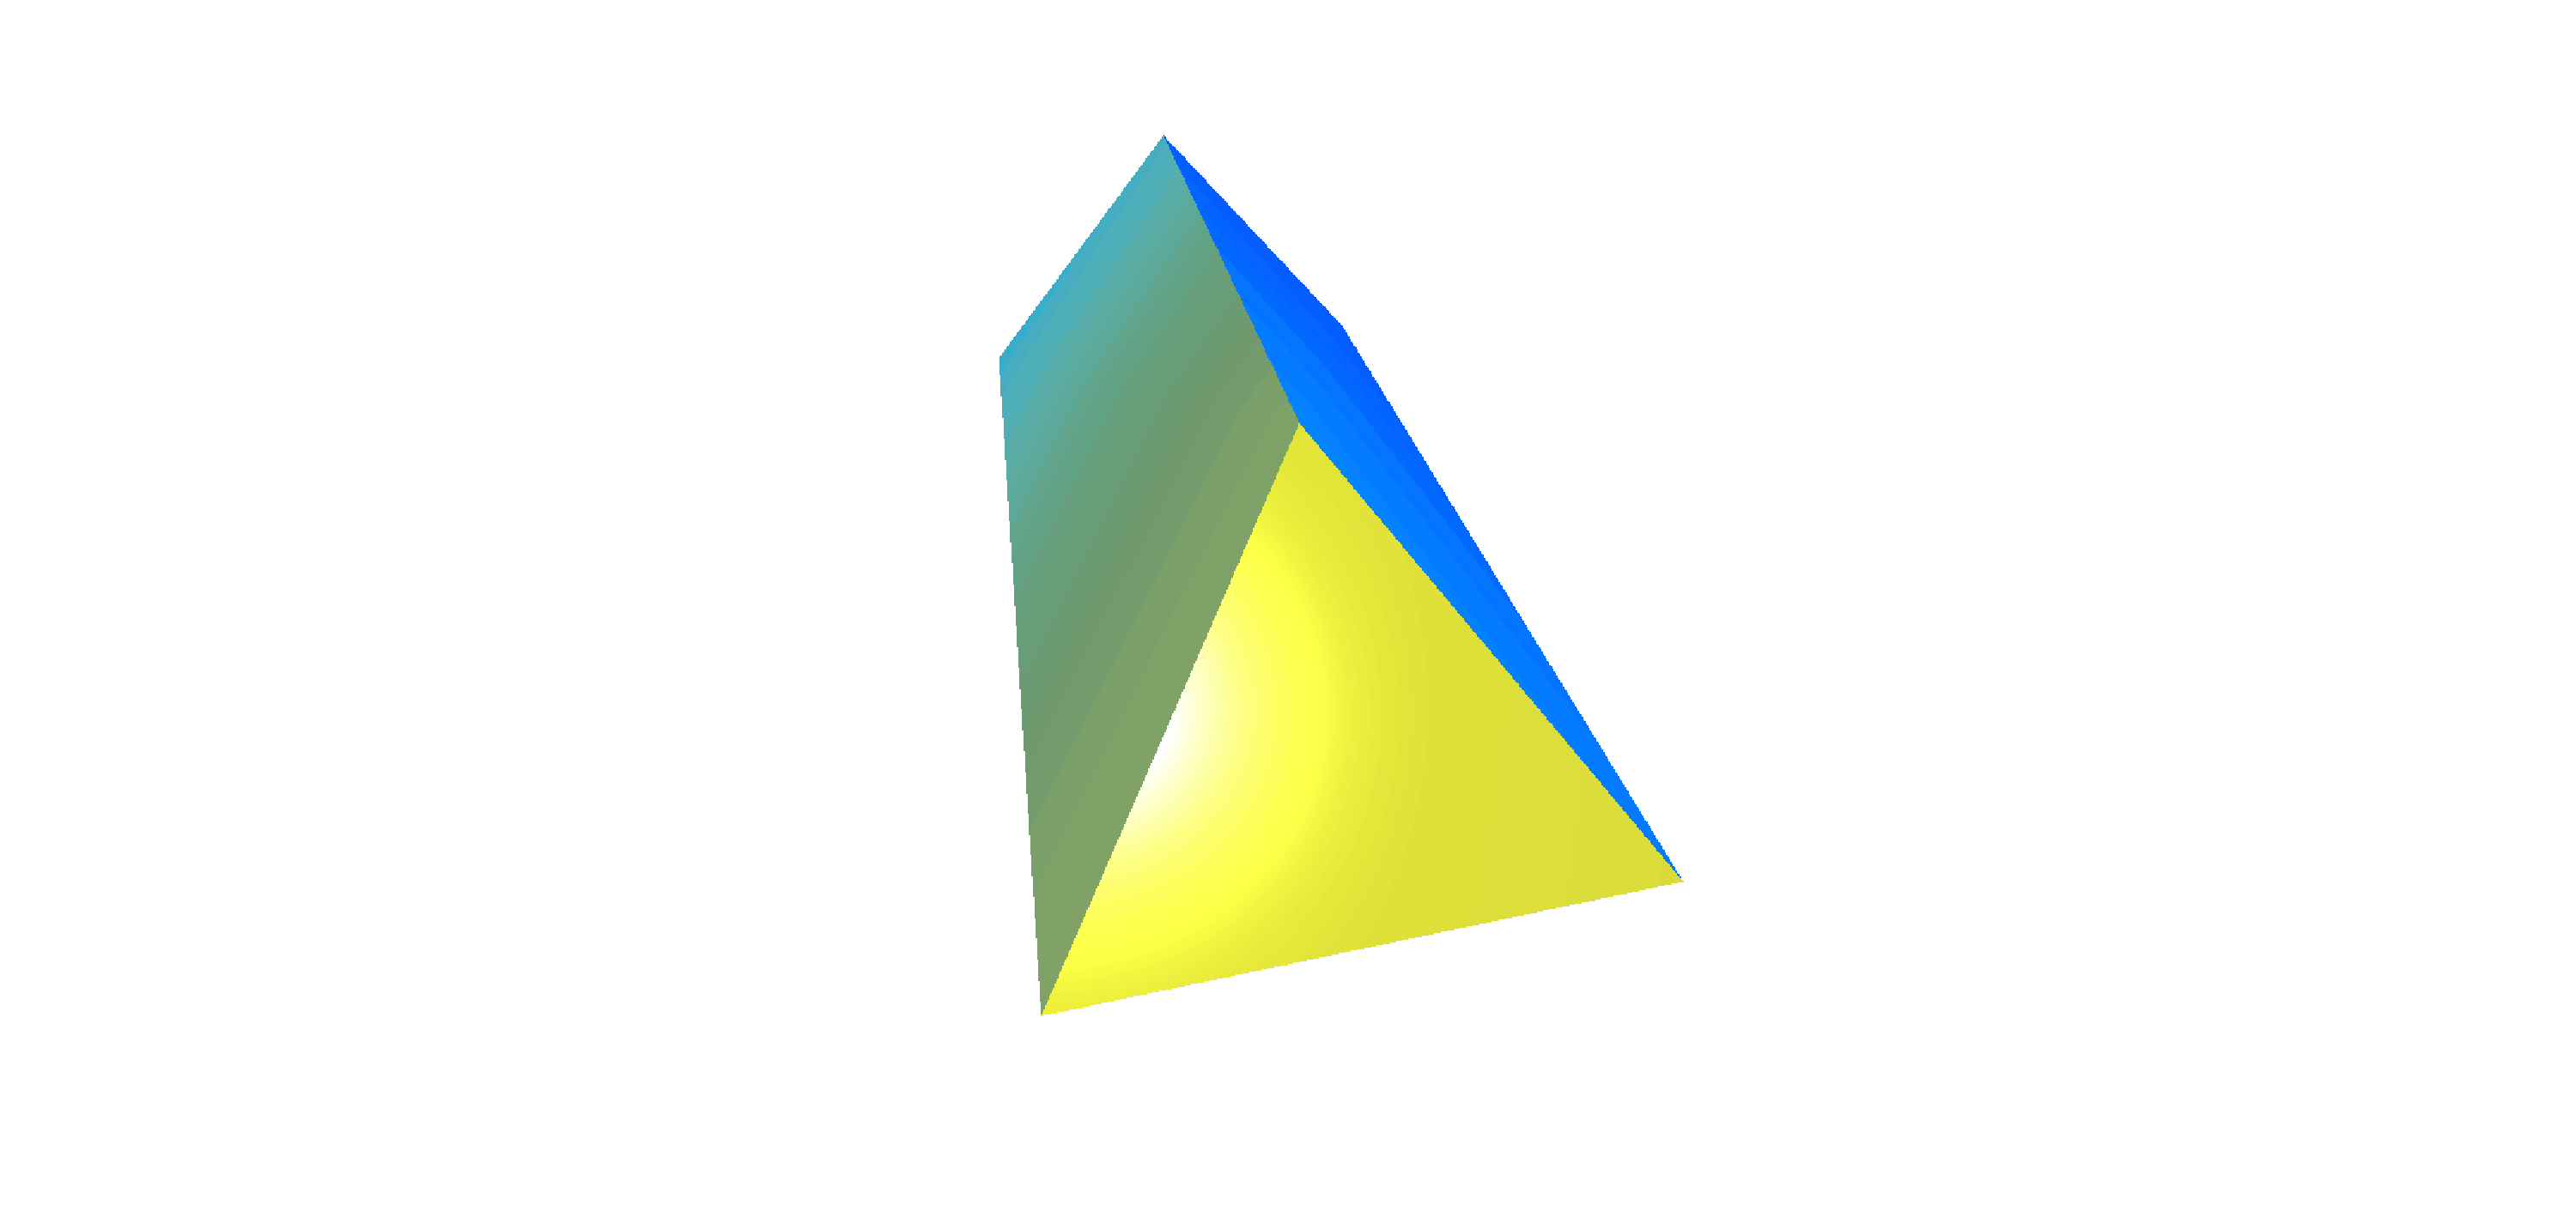
\includegraphics{Pic/PDF/BaseShape/Hip000.pdf}}}
  &
  \resizebox{0.2\textwidth}{!}{\rotatebox{0}{
  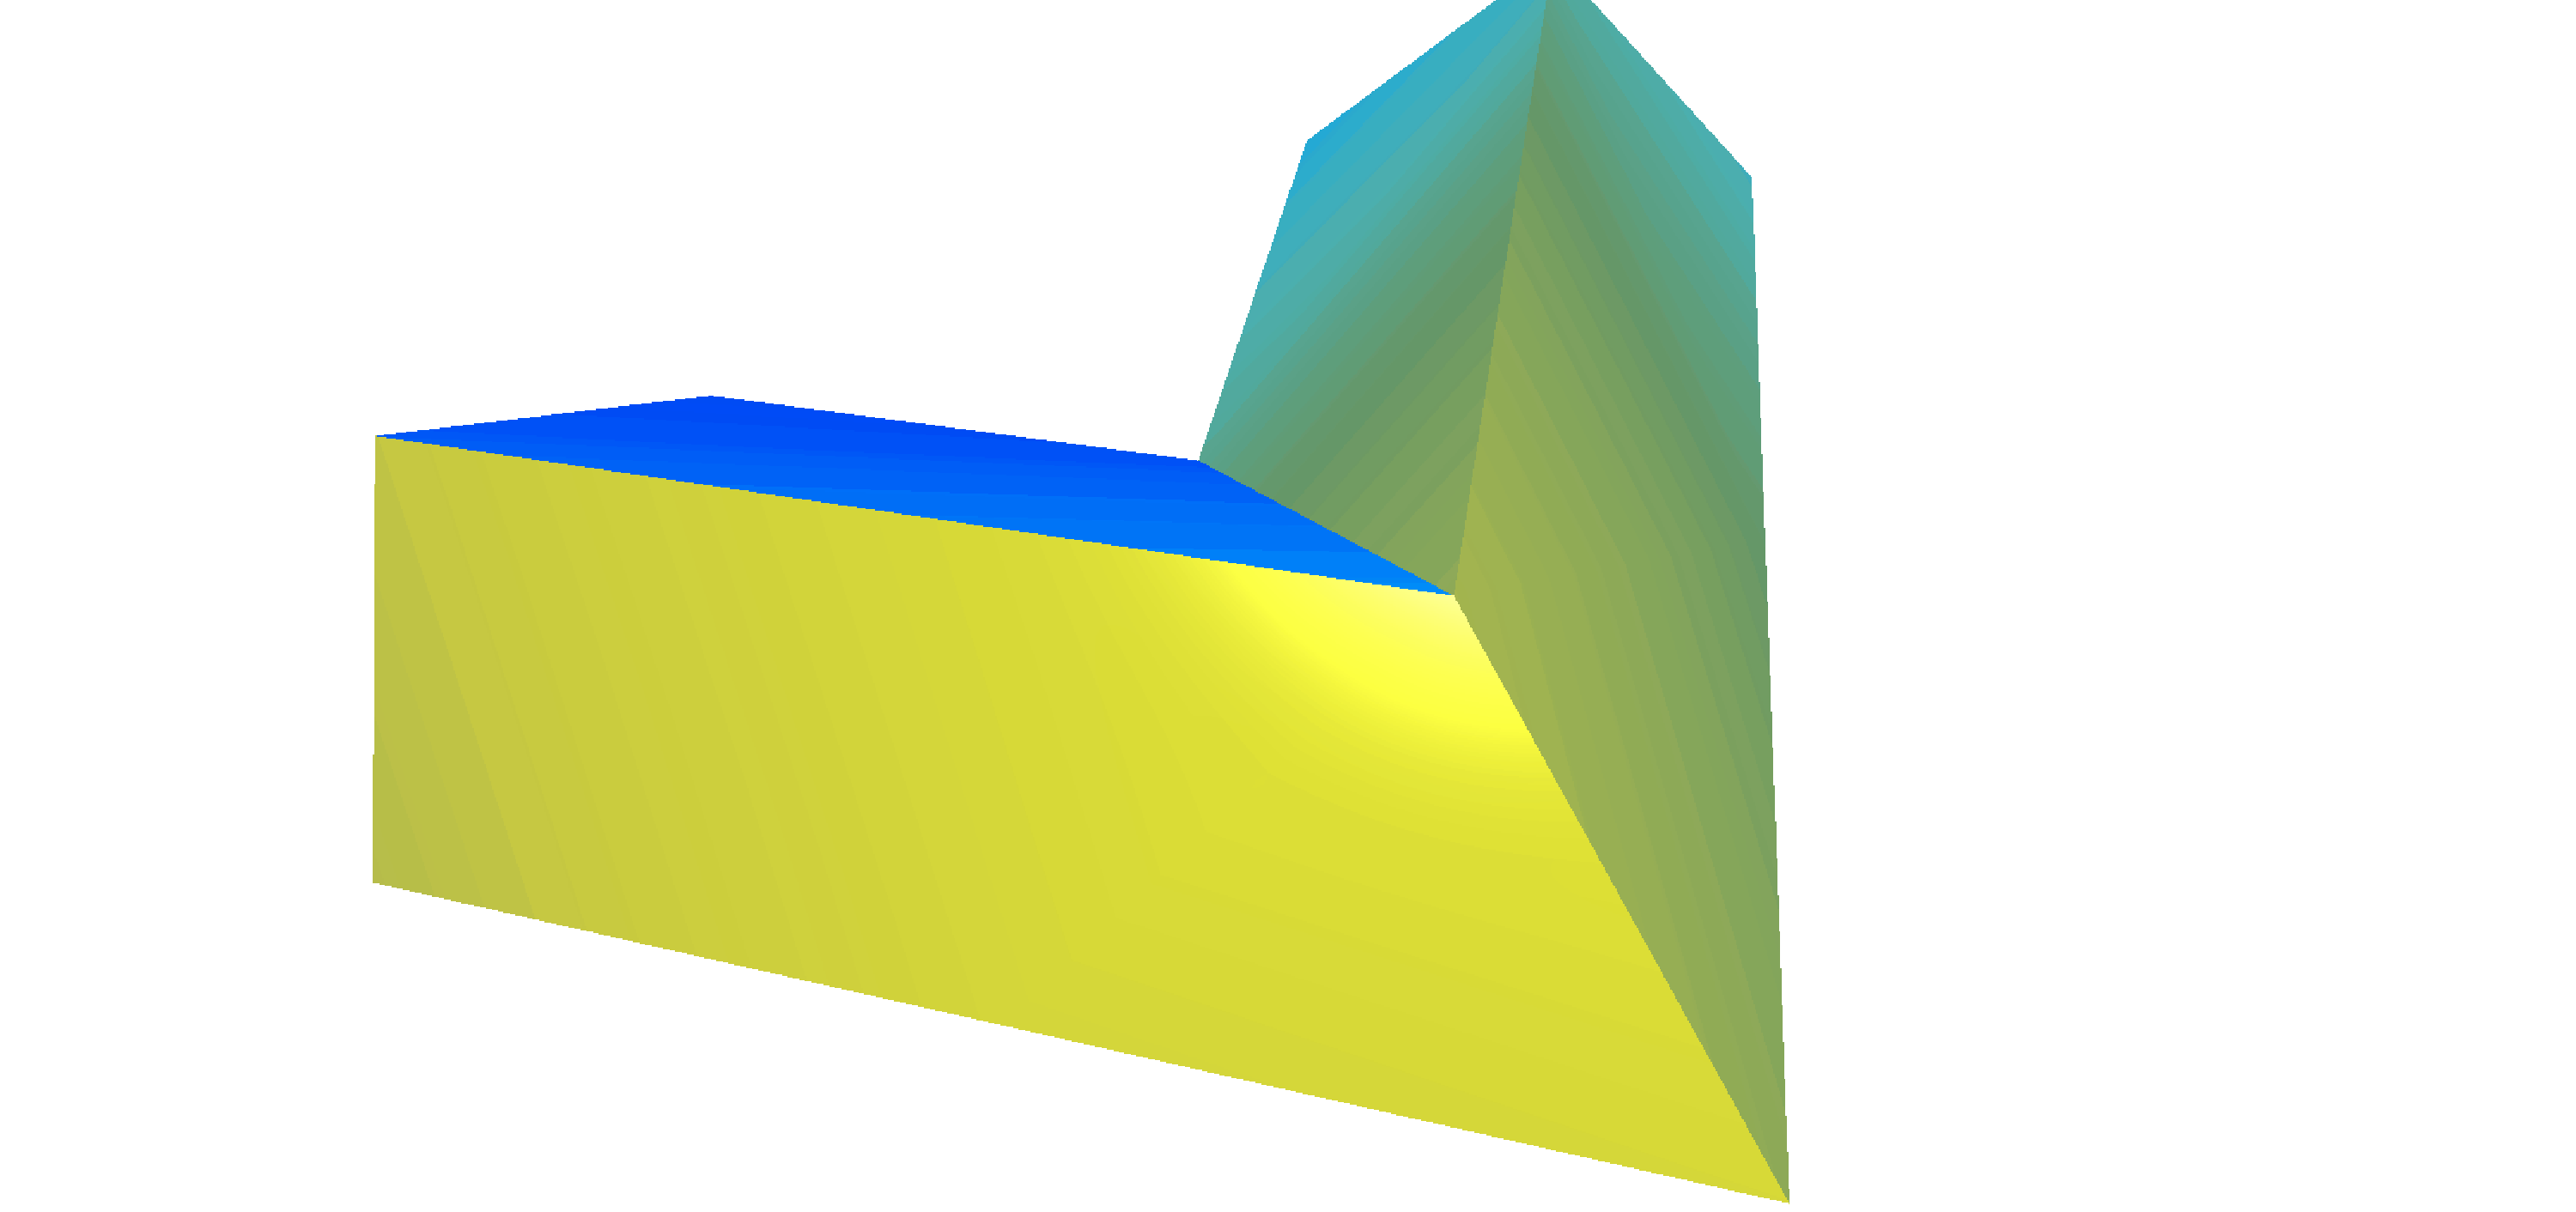
\includegraphics{Pic/PDF/BaseShape/GableL000.pdf}}}
  \\
  Flat & Gable & Hip & L-Joint
  \\
  \resizebox{0.2\textwidth}{!}{\rotatebox{0}{
  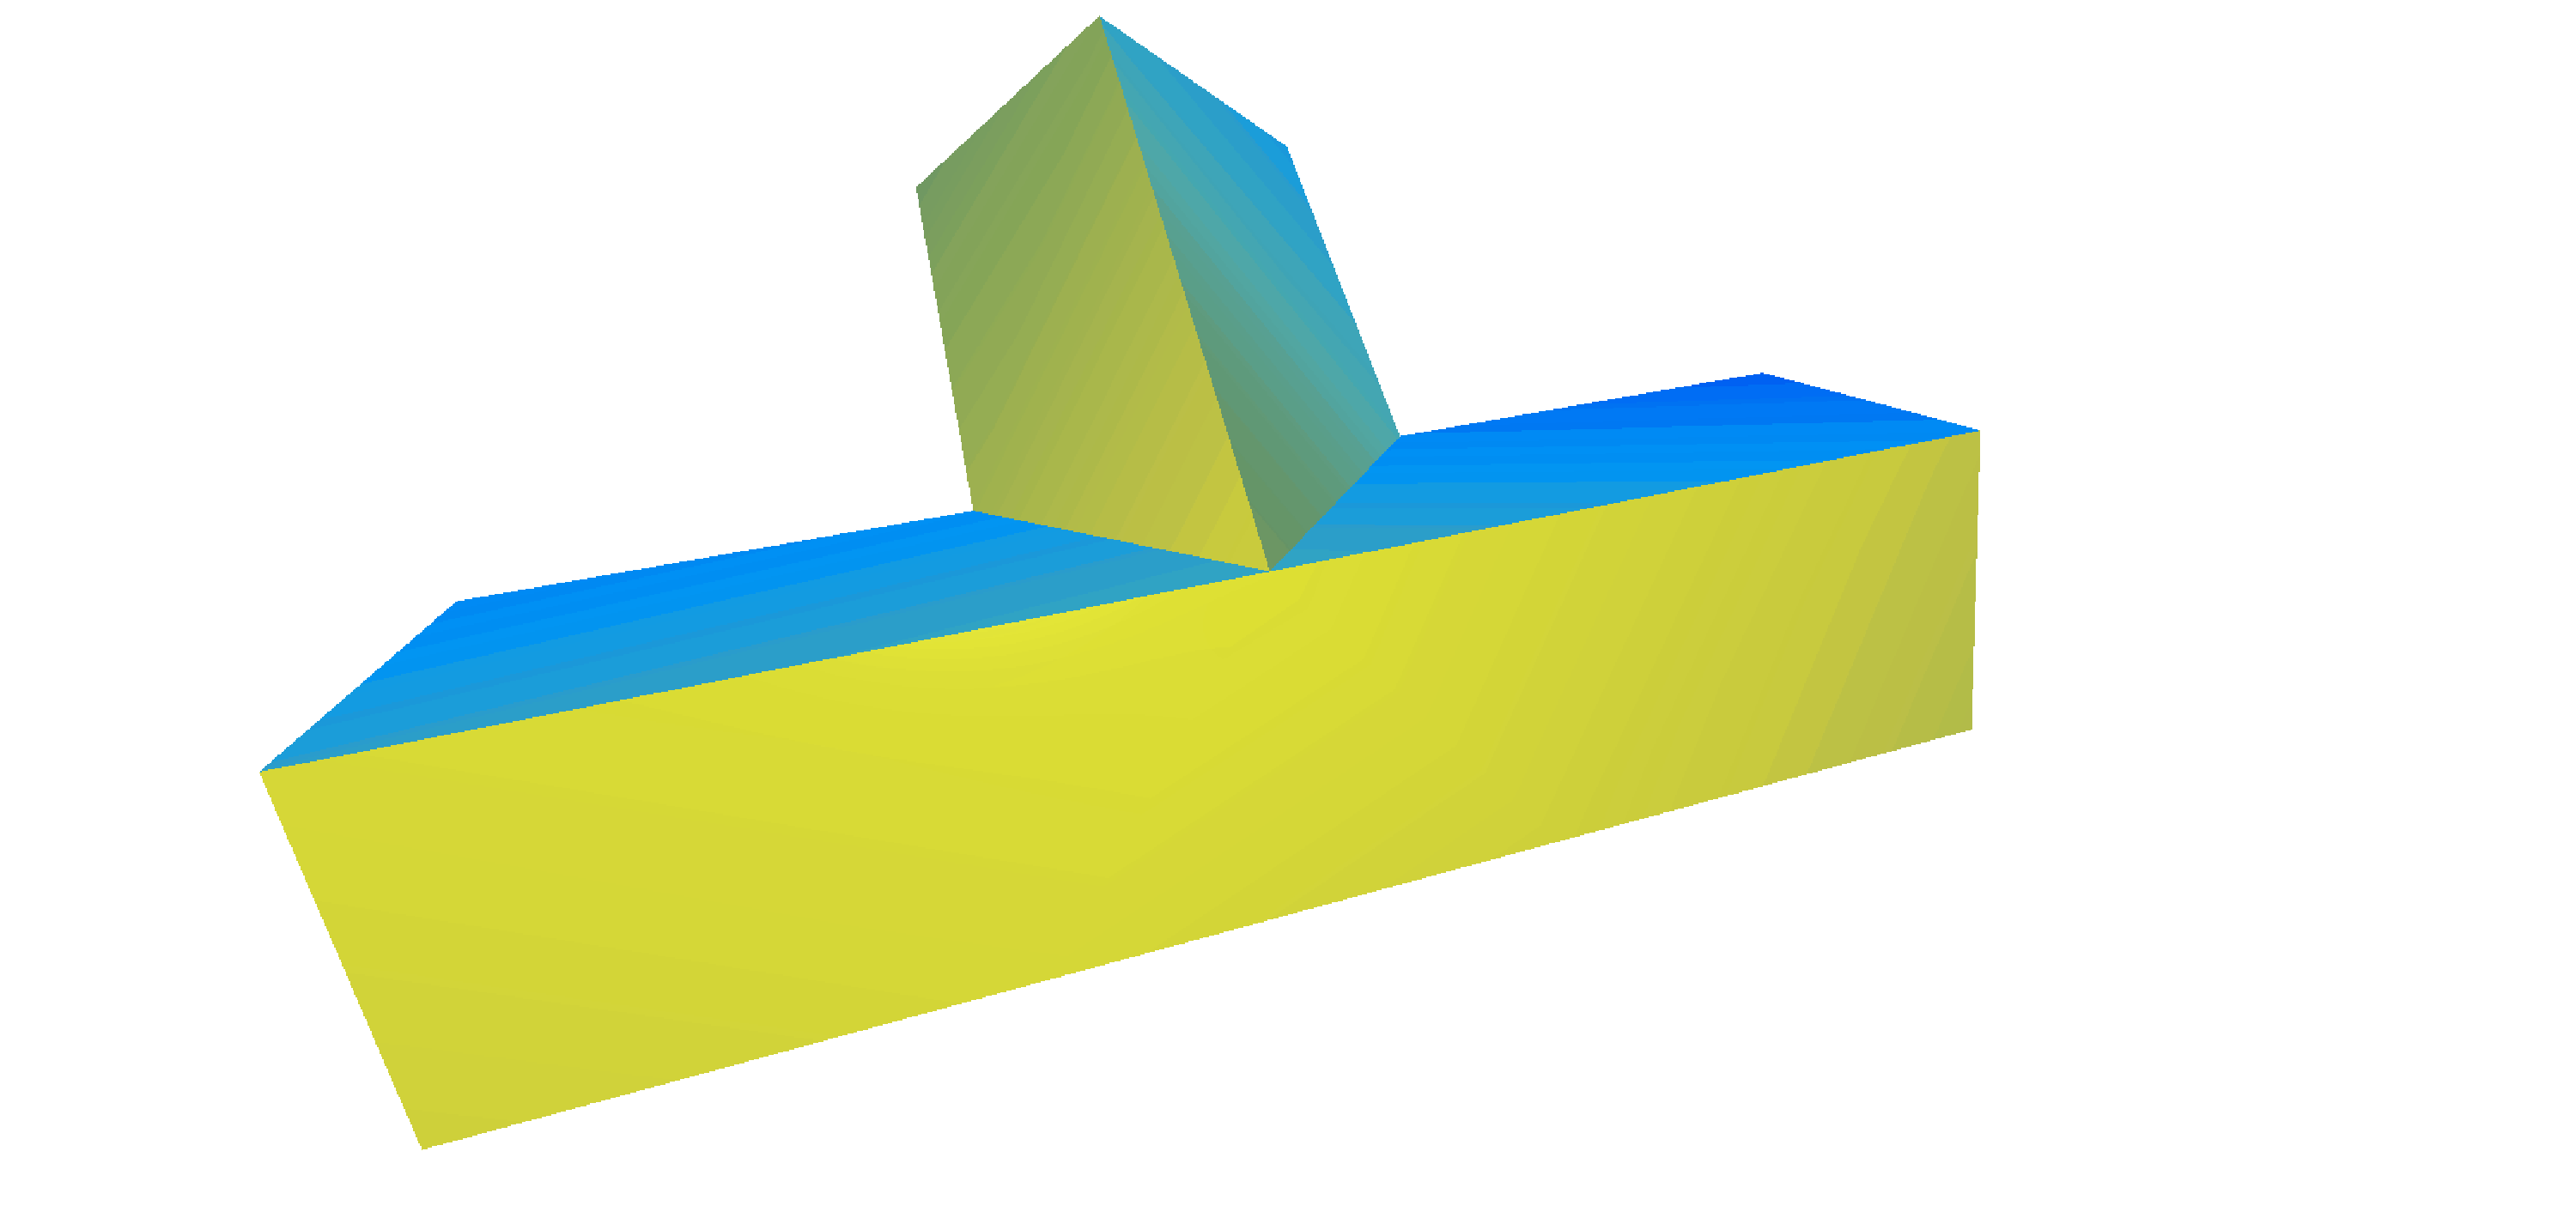
\includegraphics{Pic/PDF/BaseShape/GableT000.pdf}}}
  &
  \resizebox{0.2\textwidth}{!}{\rotatebox{0}{
  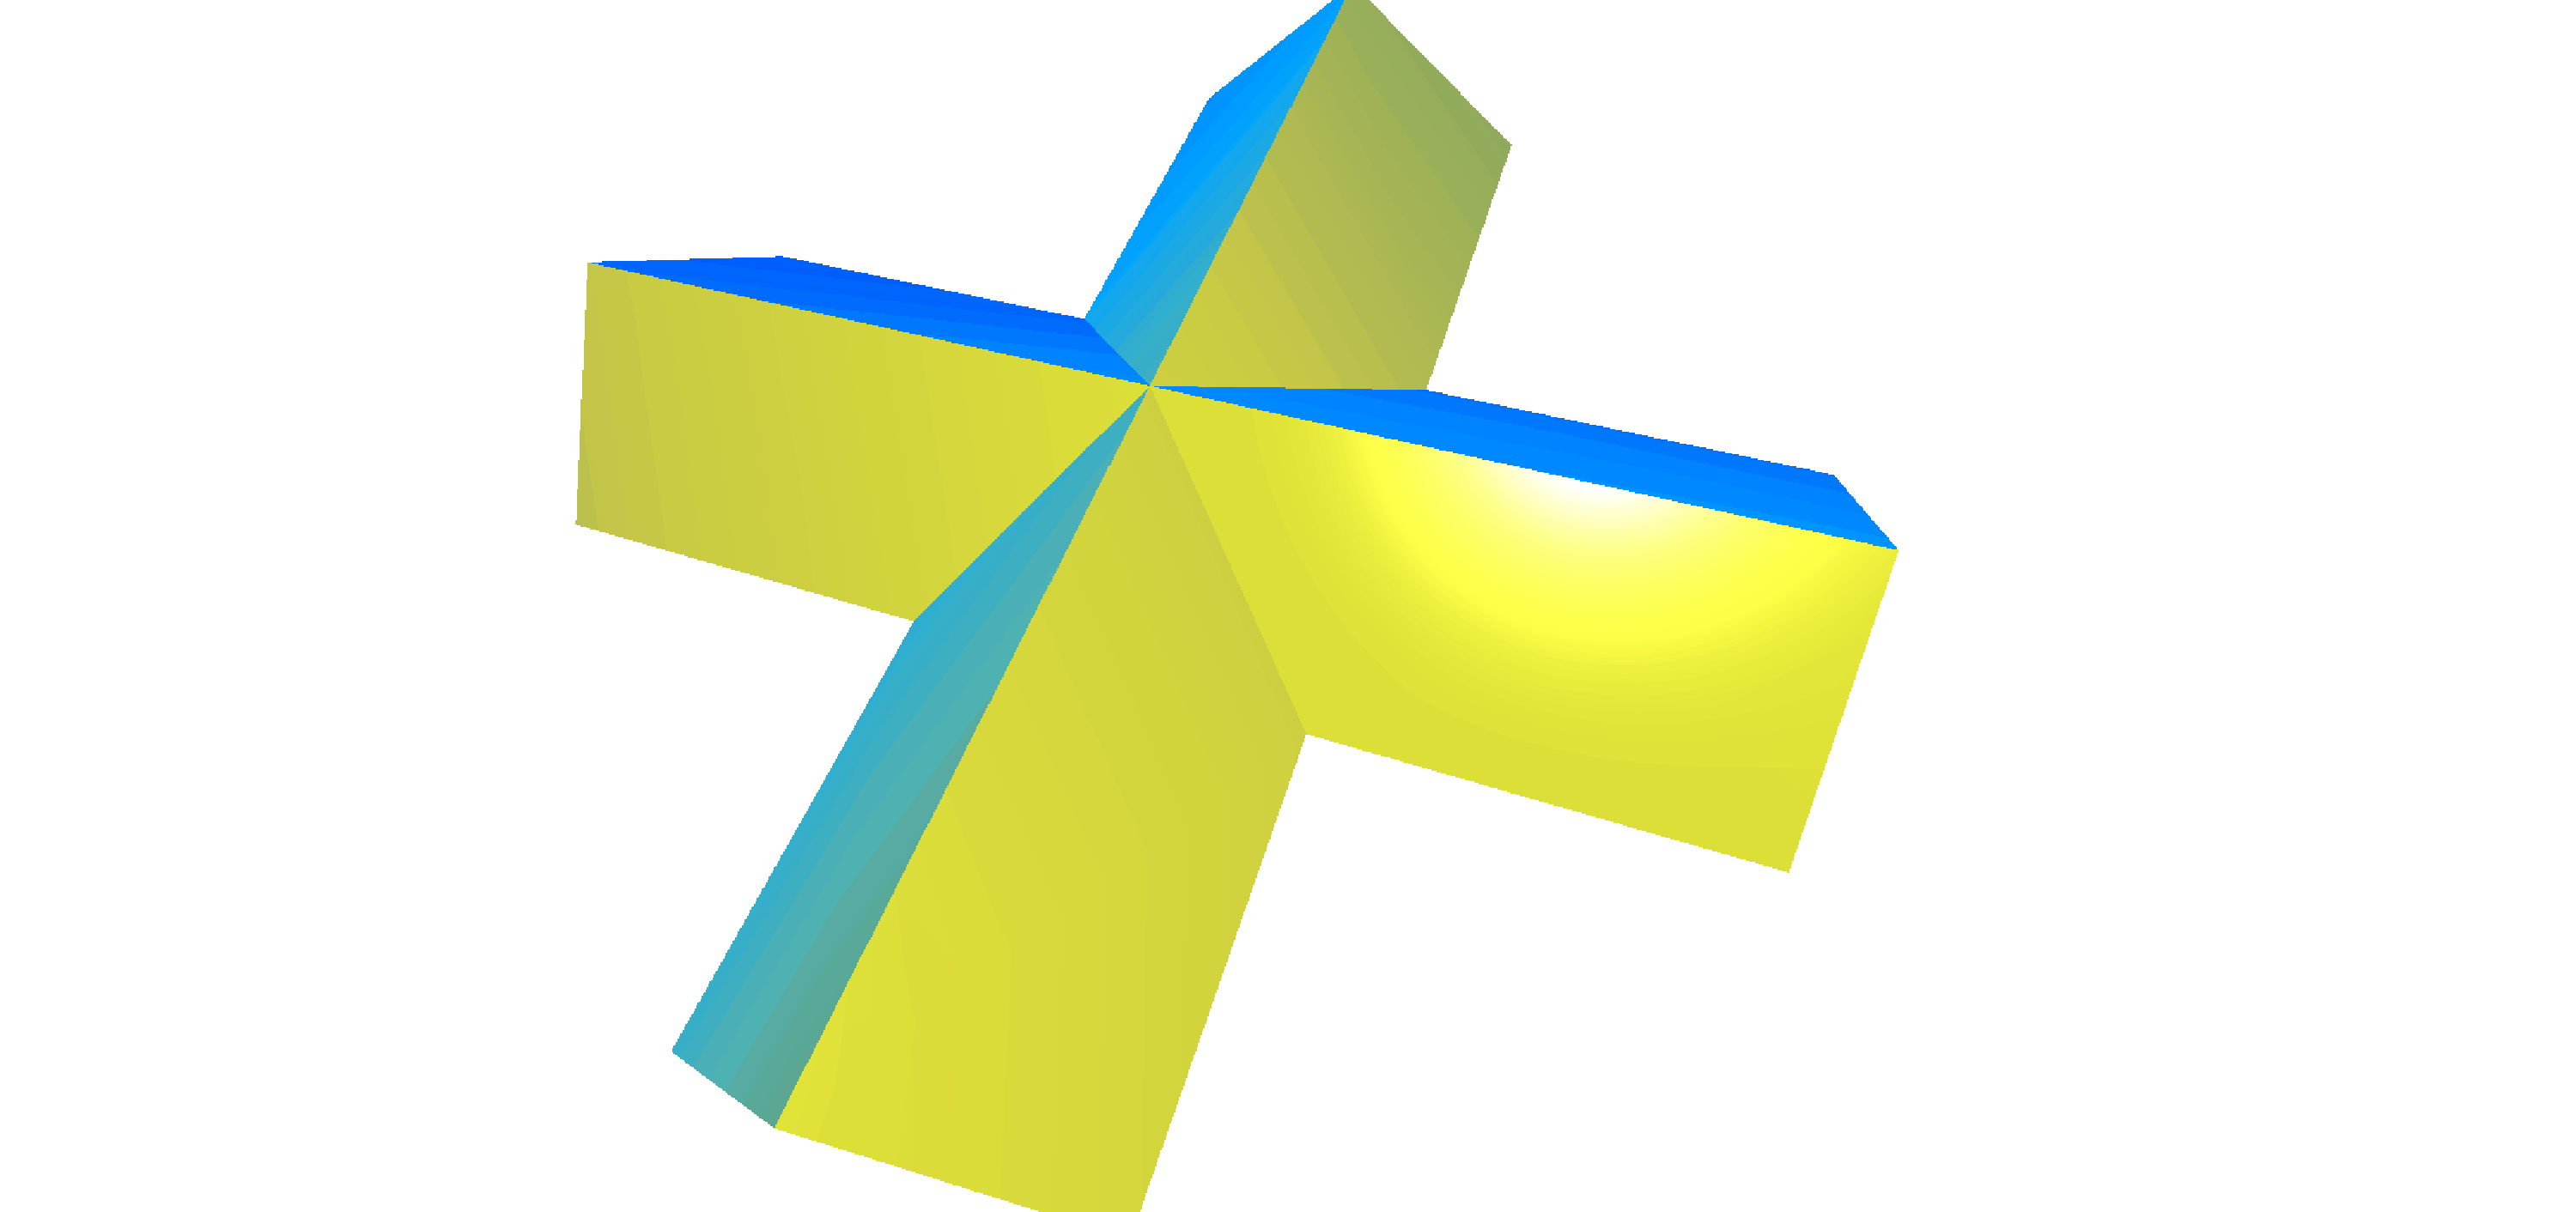
\includegraphics{Pic/PDF/BaseShape/GableX000.pdf}}}
  &
  \resizebox{0.2\textwidth}{!}{\rotatebox{0}{
  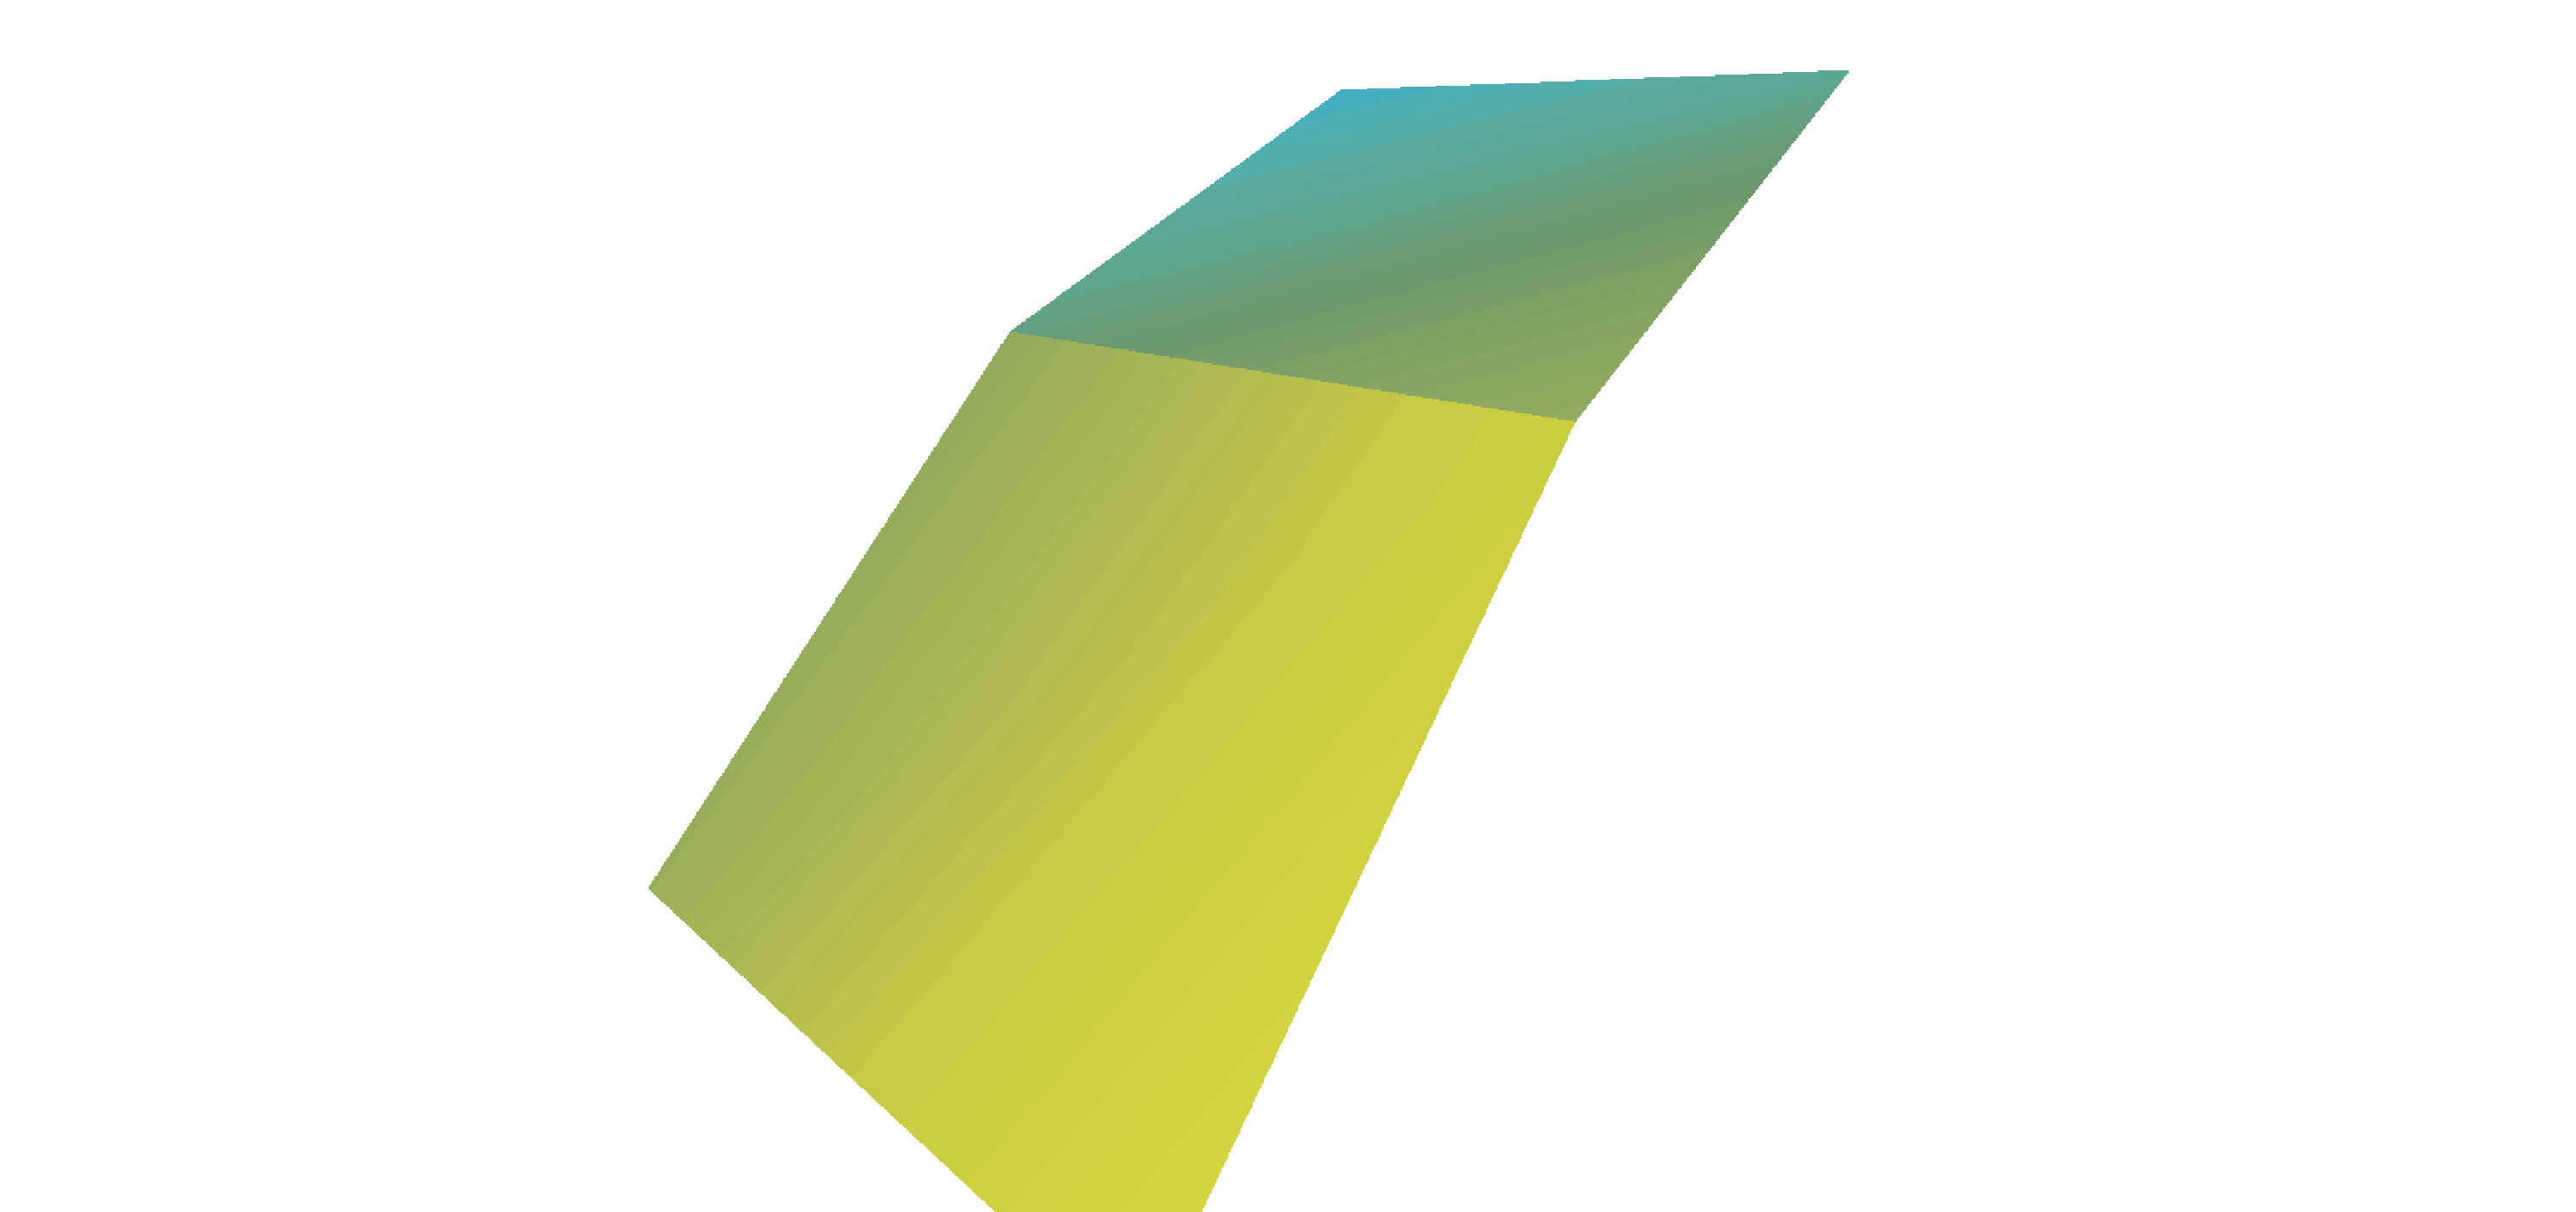
\includegraphics{Pic/PDF/BaseShape/Gambrel000.pdf}}}
  &
  \resizebox{0.2\textwidth}{!}{\rotatebox{0}{
  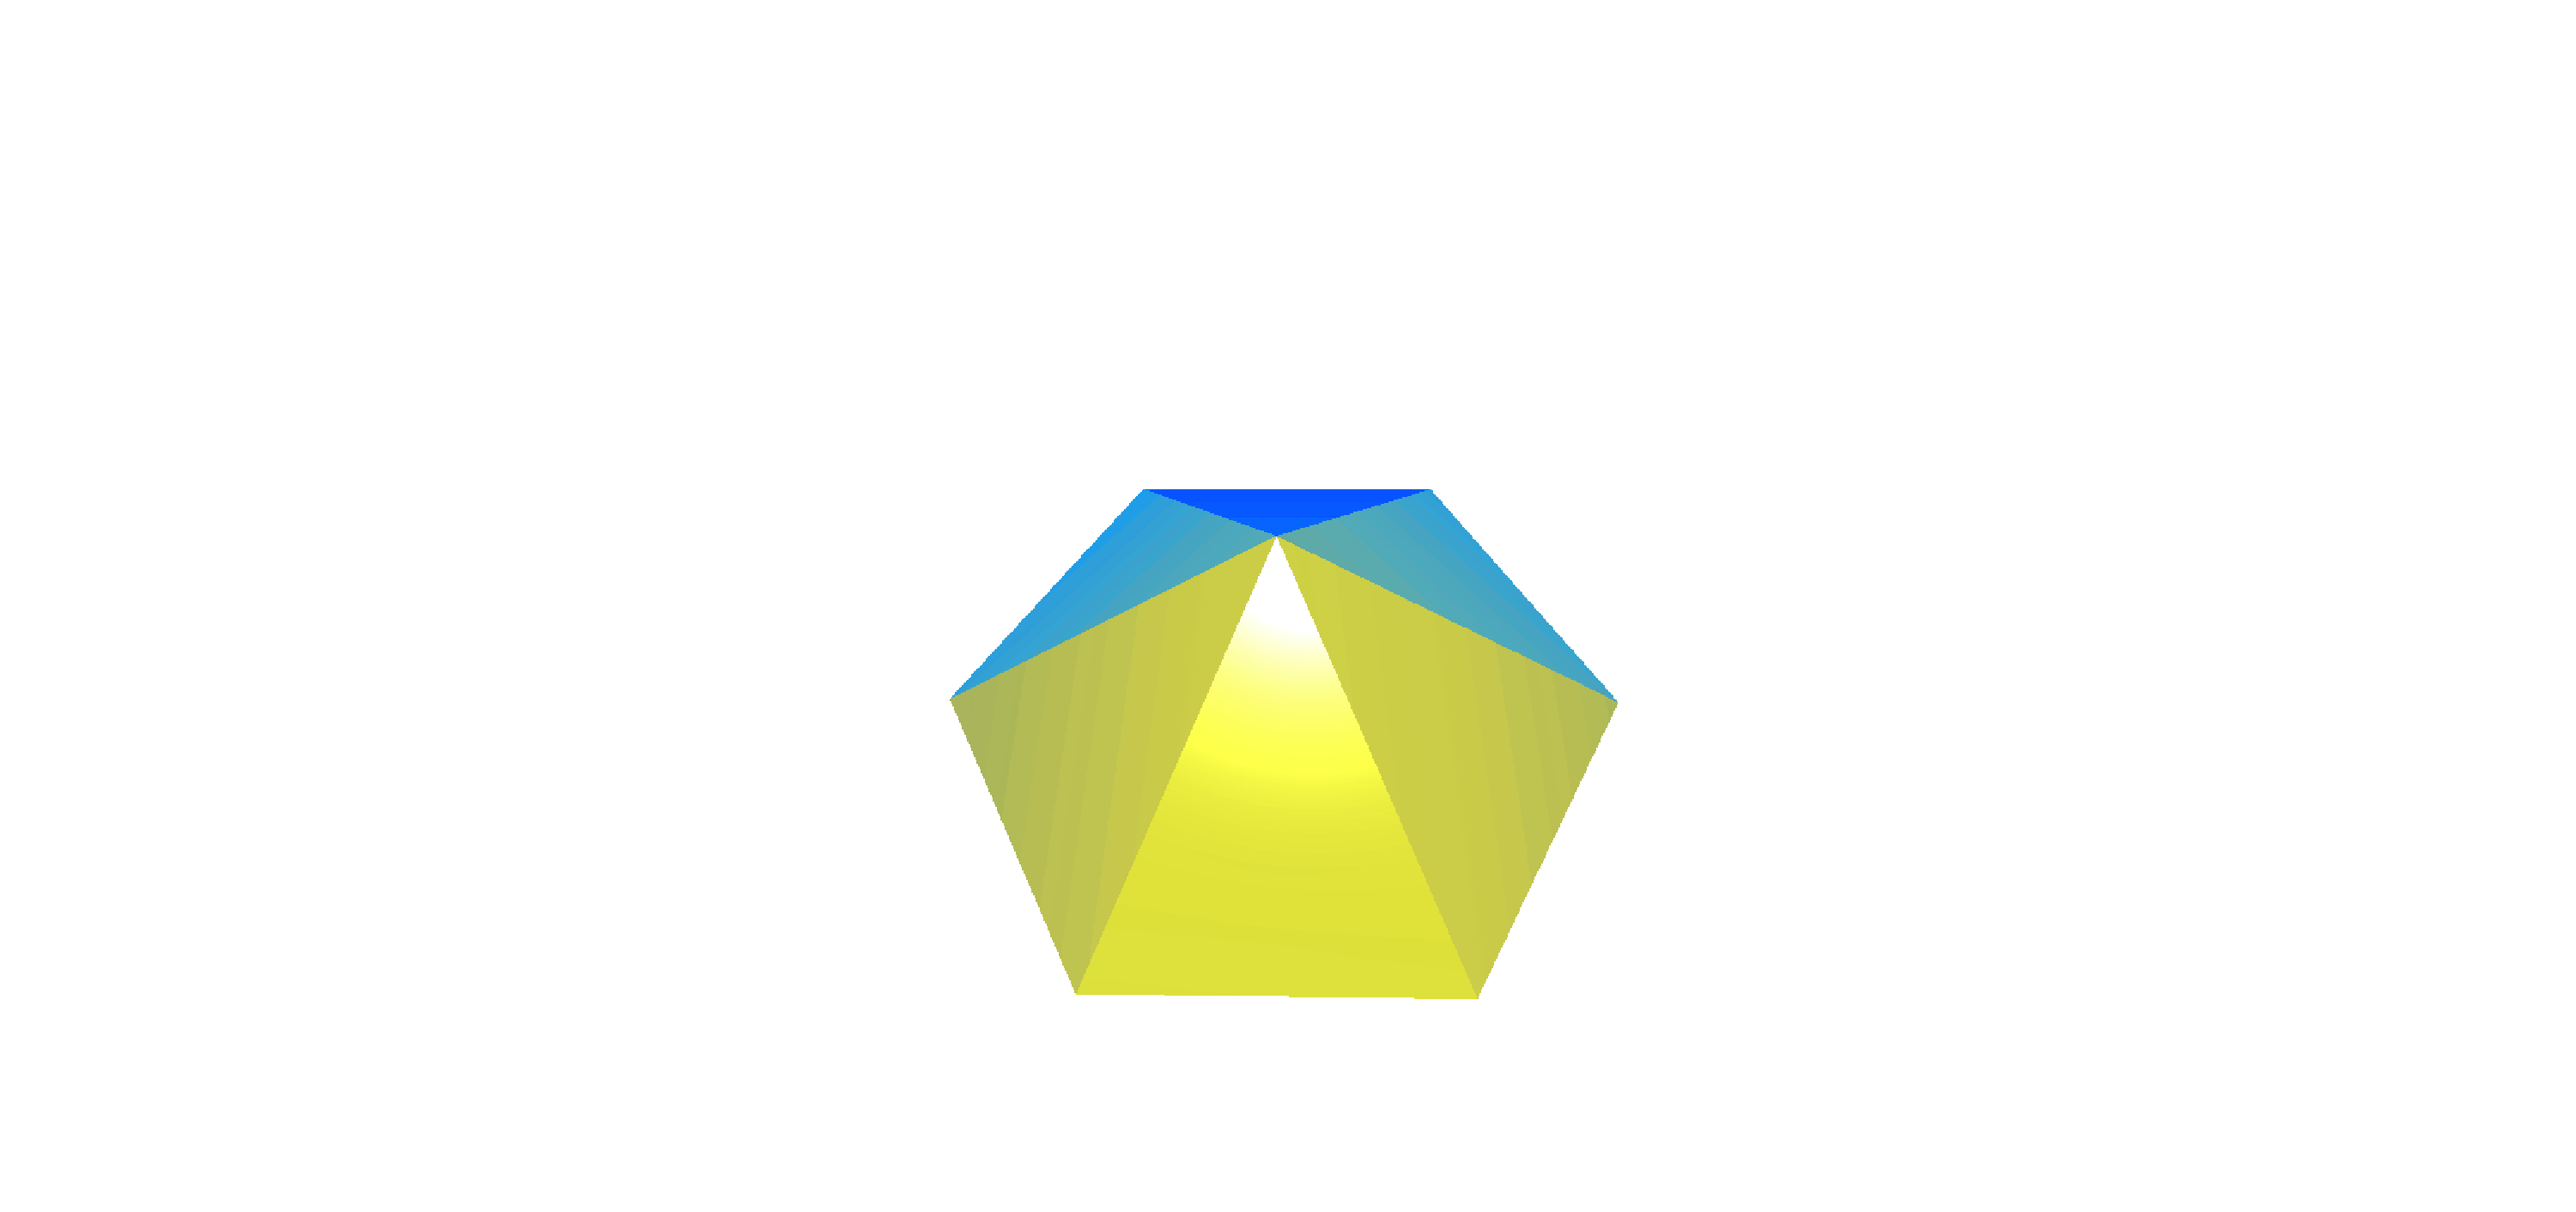
\includegraphics{Pic/PDF/BaseShape/Hex000.pdf}}}
  \\
  T-Joint & X-Joint & Gambrel & Hex
  \\
  \resizebox{0.2\textwidth}{!}{\rotatebox{0}{
  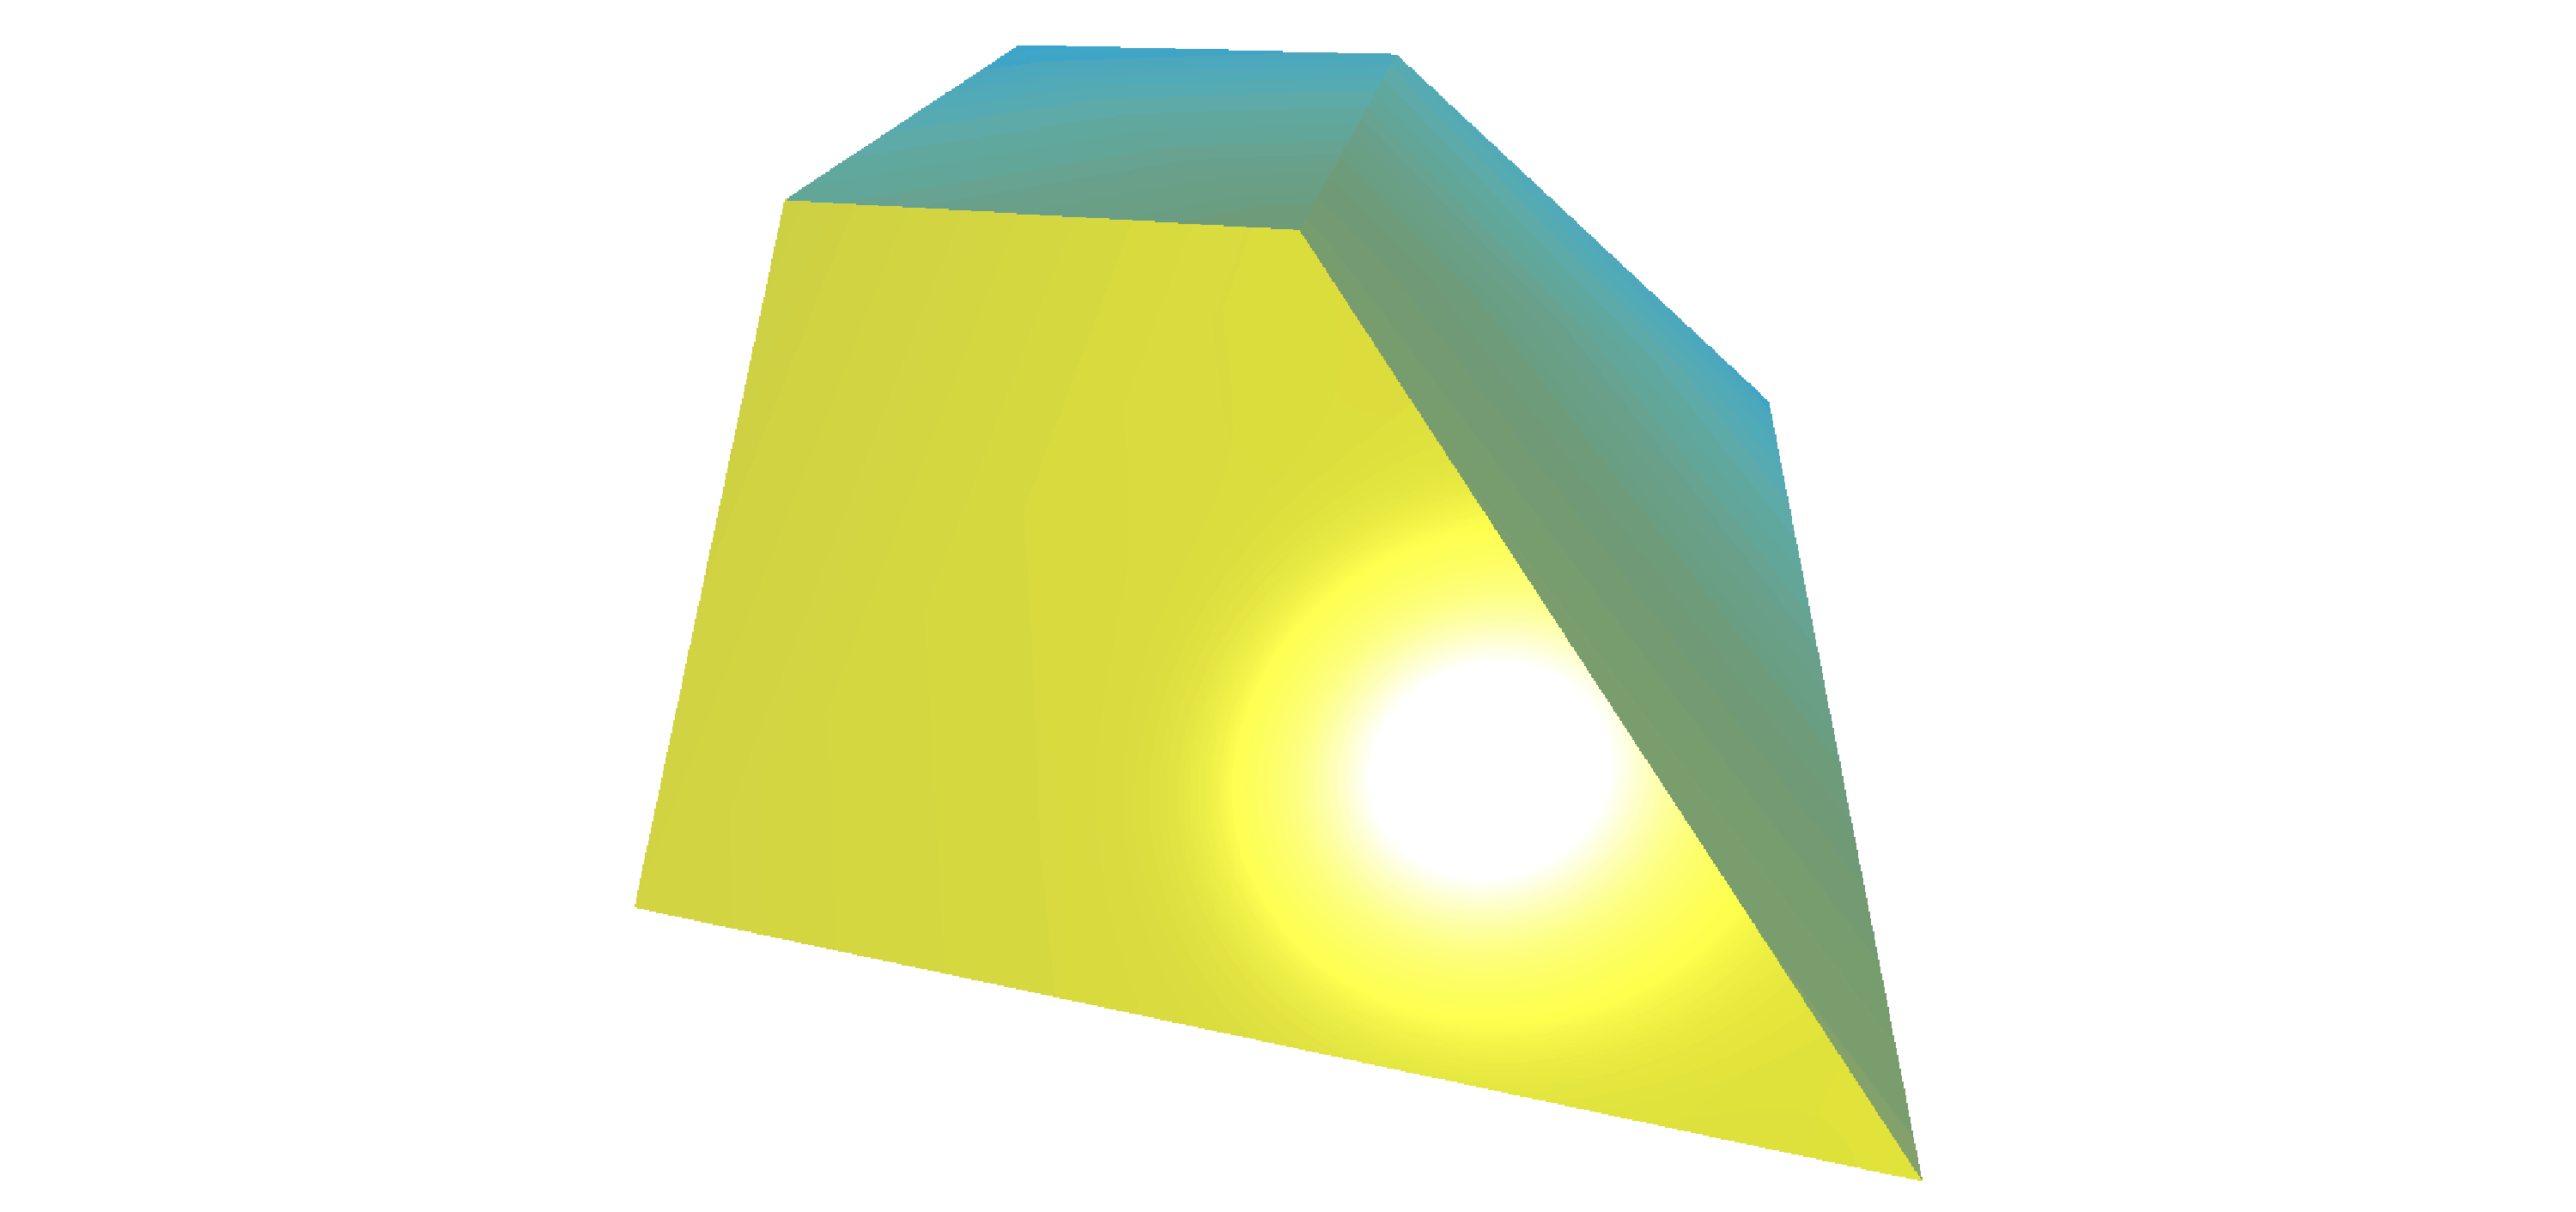
\includegraphics{Pic/PDF/BaseShape/Mansard000.pdf}}}
  &
  \resizebox{0.2\textwidth}{!}{\rotatebox{0}{
  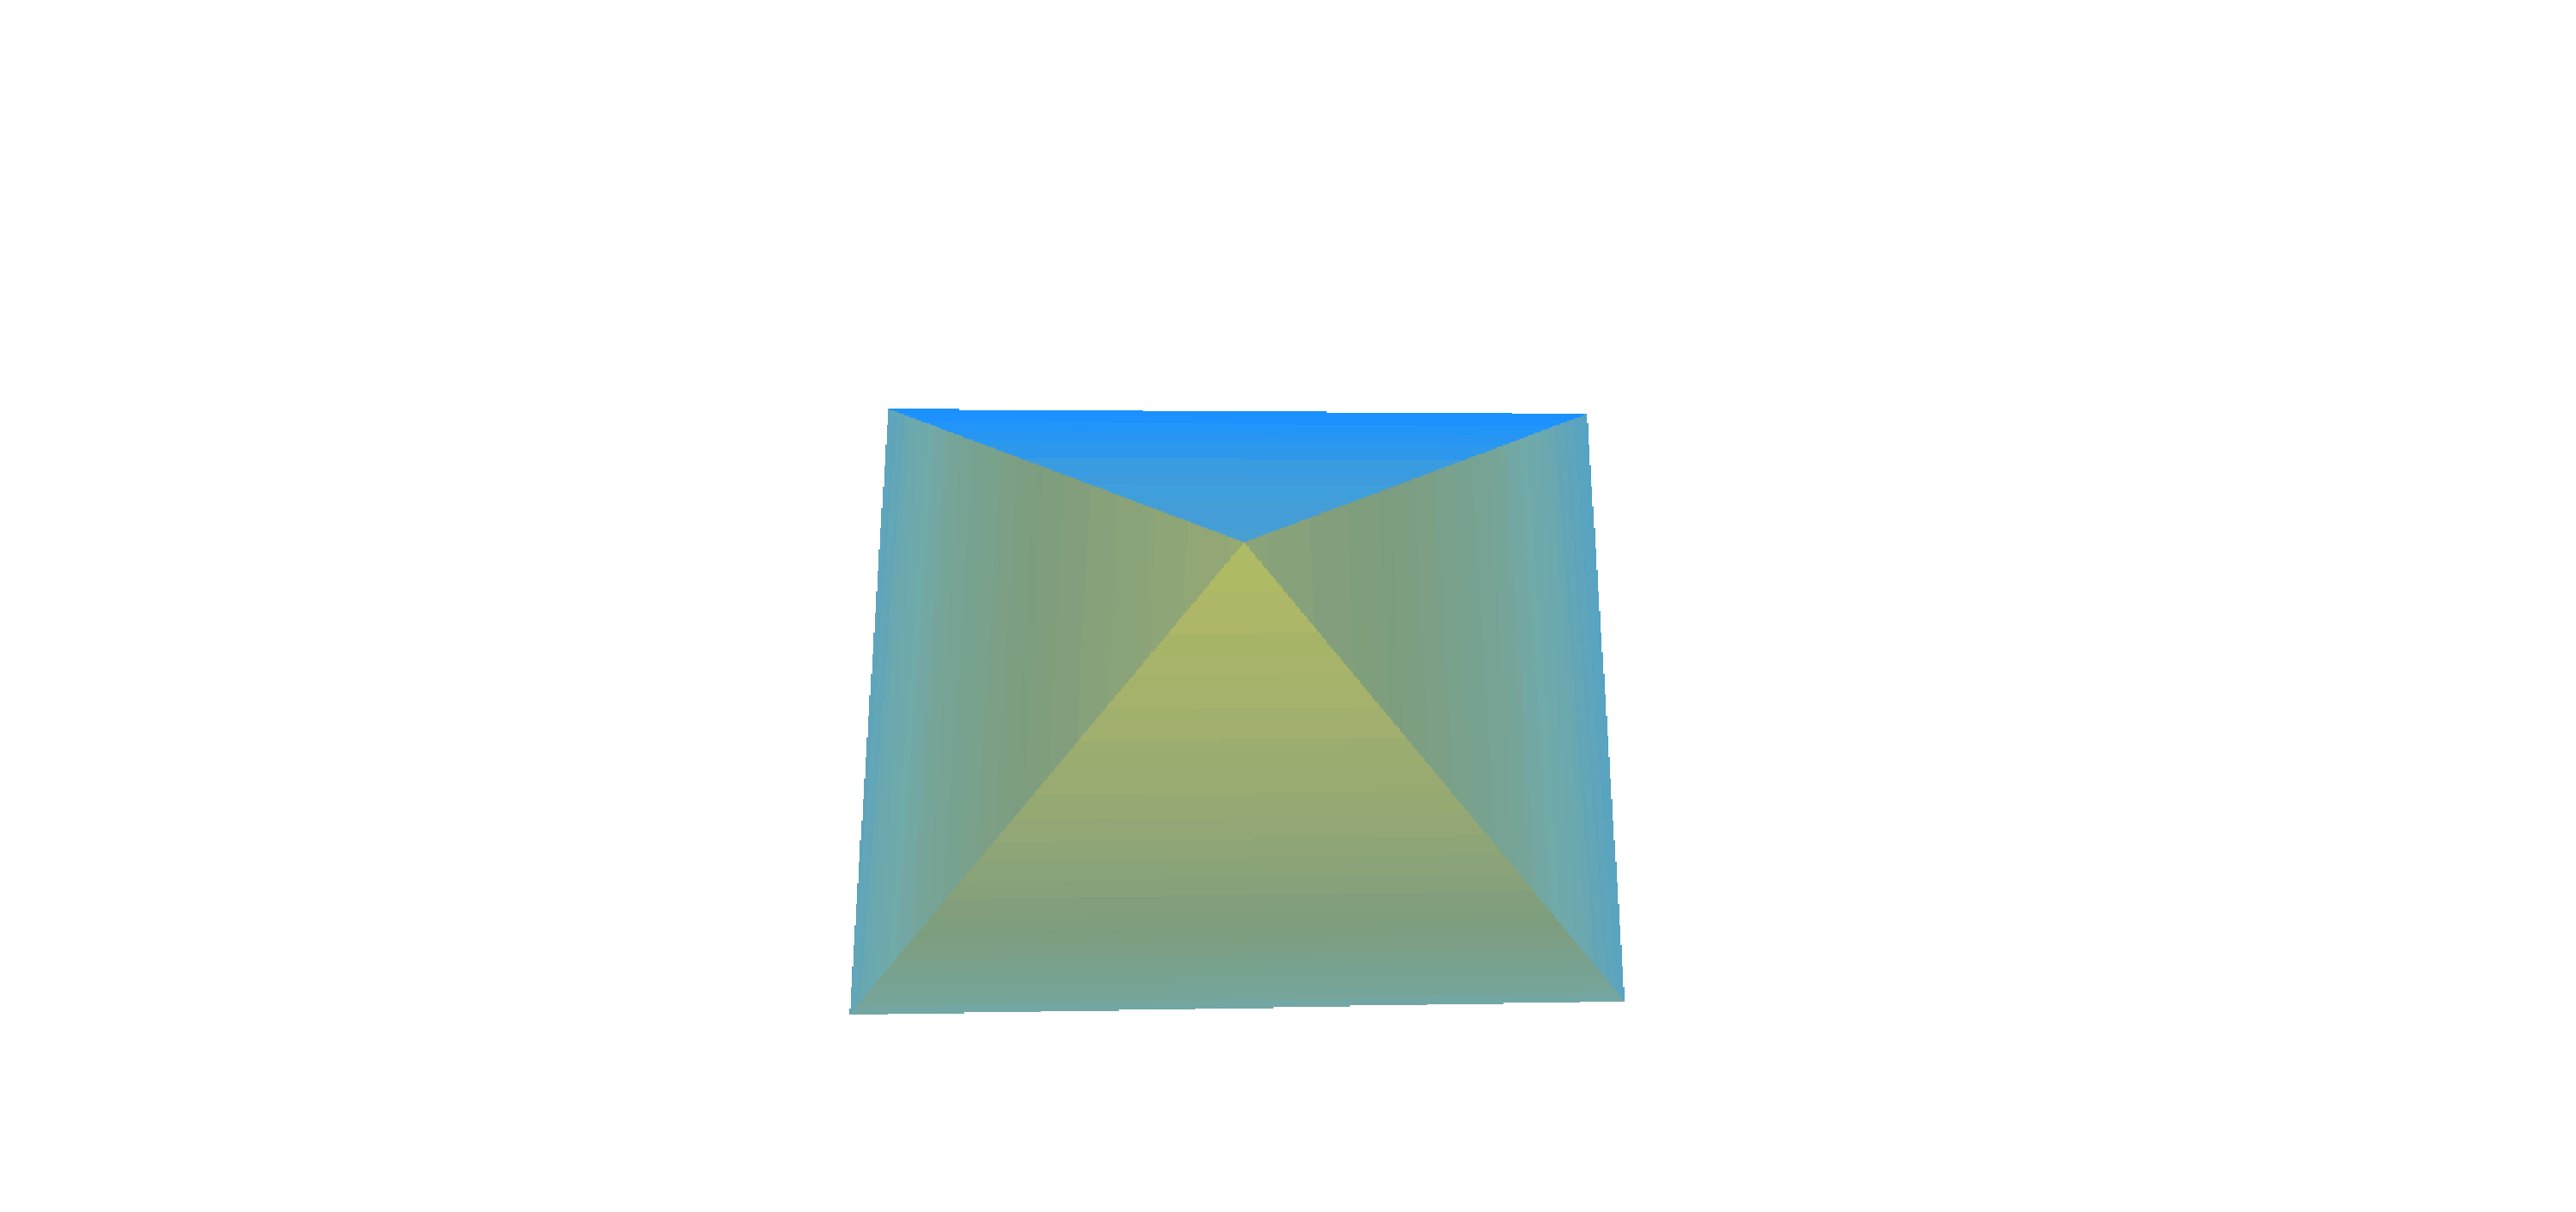
\includegraphics{Pic/PDF/BaseShape/Pyramid000.pdf}}}
  &
  \resizebox{0.2\textwidth}{!}{\rotatebox{0}{
  
\includegraphics{Pic/PDF/BaseShape/Shed000.pdf}}}
  &
  \resizebox{0.2\textwidth}{!}{\rotatebox{0}{
  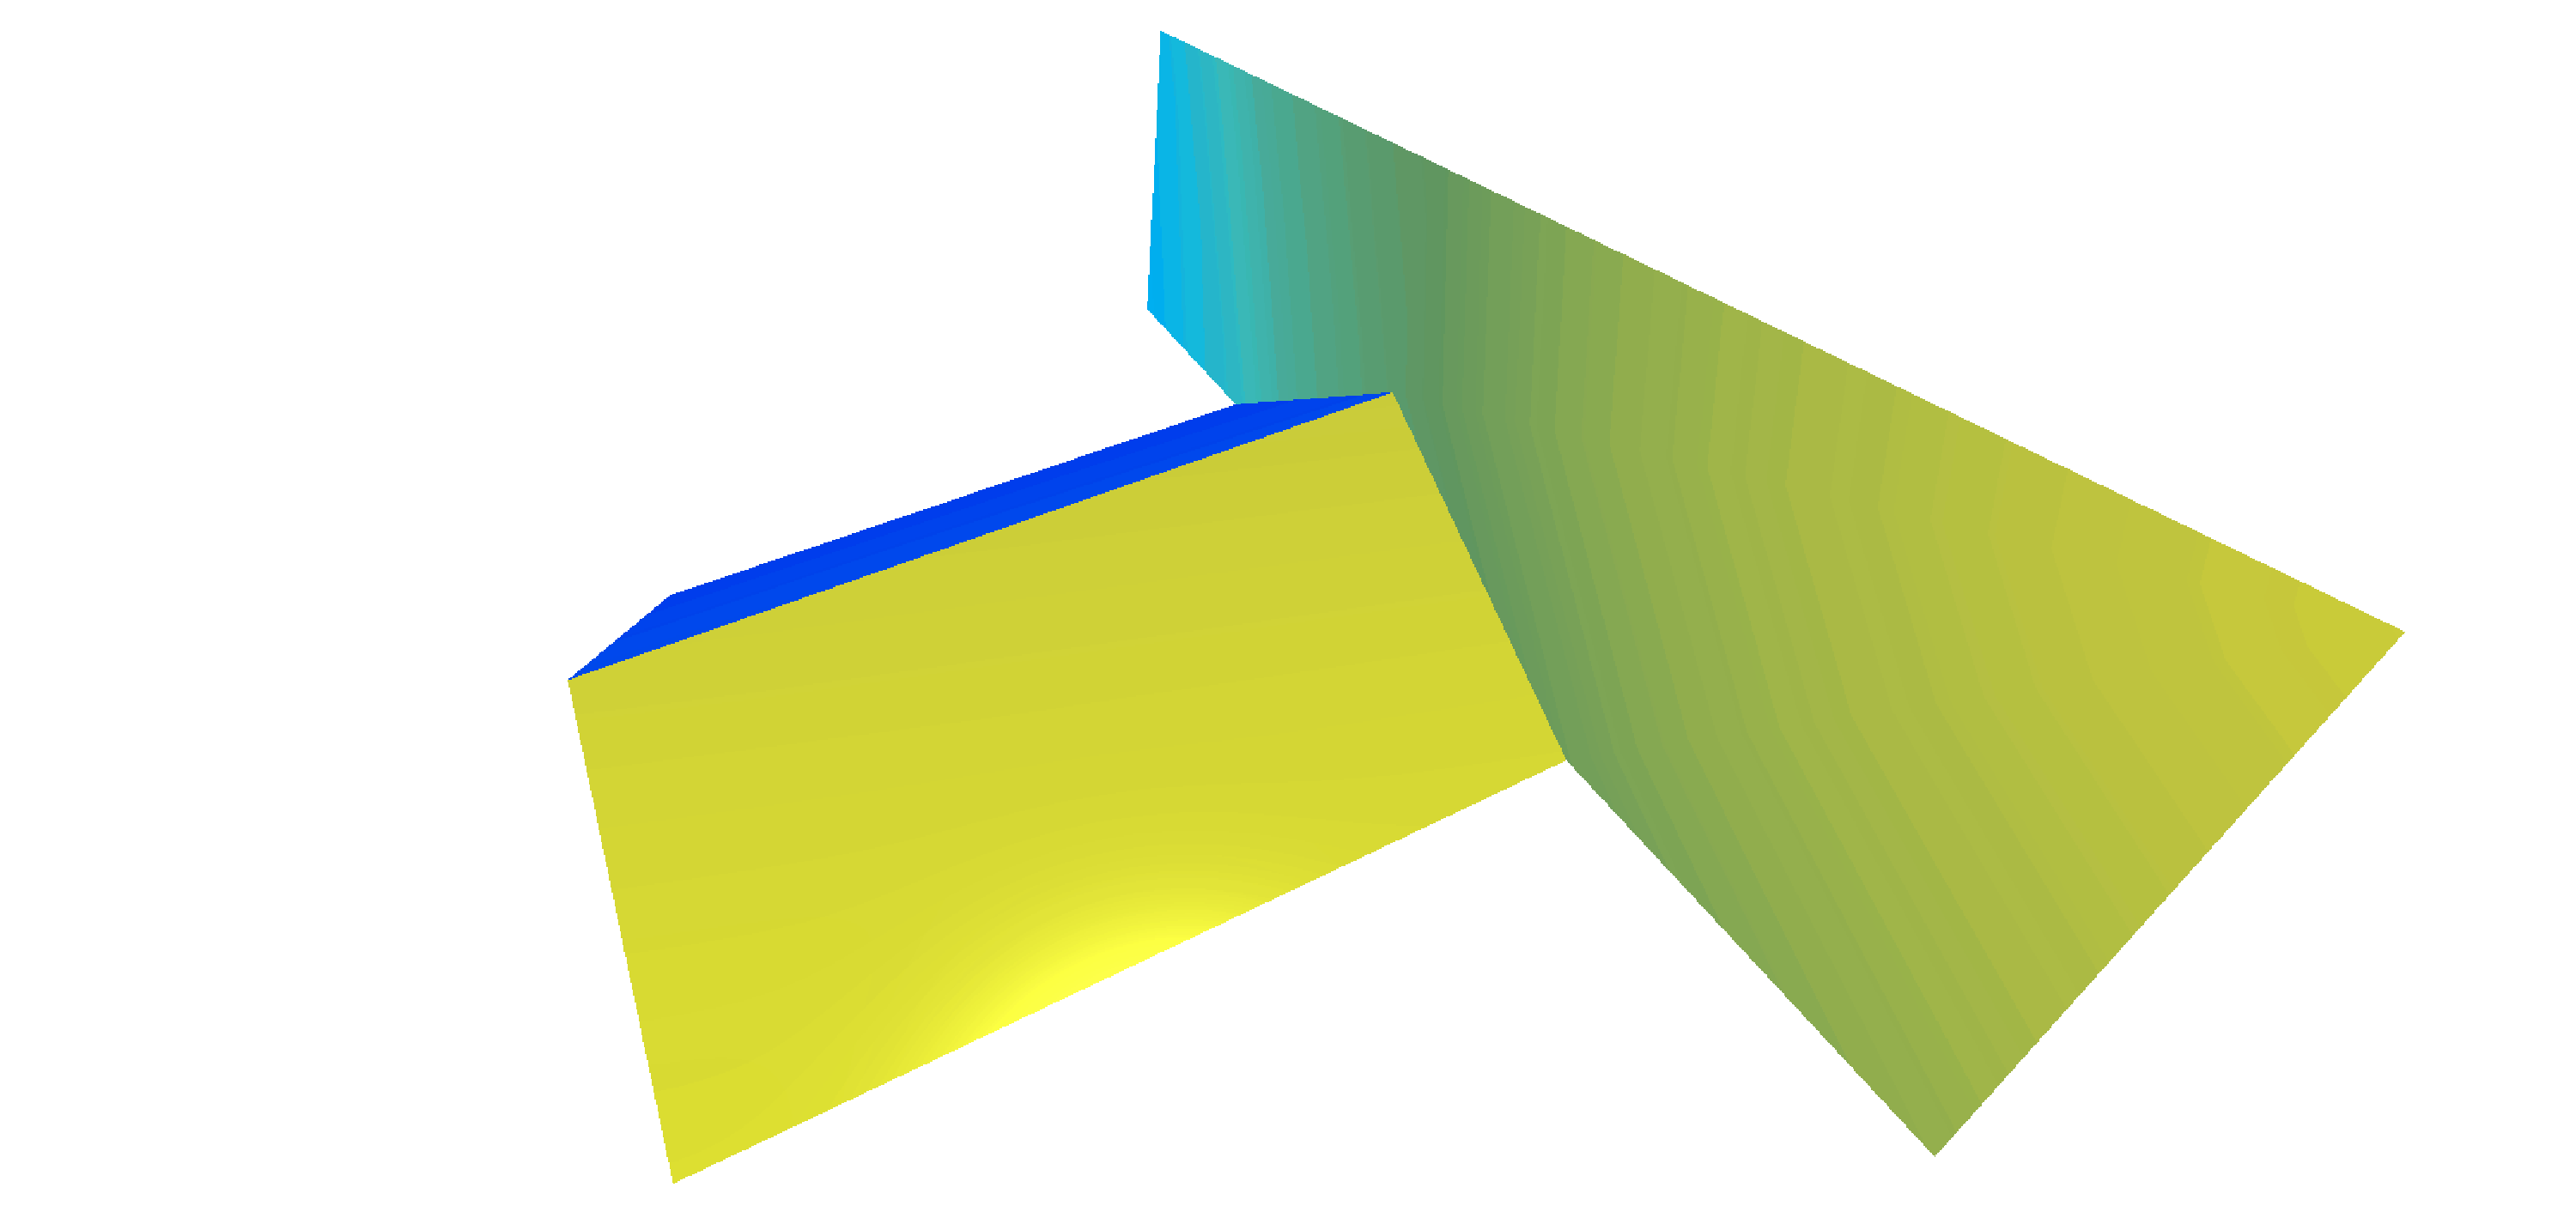
\includegraphics{Pic/PDF/BaseShape/ShedGable000.pdf}}}
  \\
  Mansard & Pyramid & Shed & Loft
\end{tabular}}
\caption{Illustration of all roof base models that are used in this work.}
\label{fig: baseroofs}
\end{figure}

The difficulty in this work is to produce a codebook of important roof points. This codebook can then be used for a bag of words recognition. Learning these codebook using unsupervised learning is most straight forward. However, unsupervised learning is often misguided easily by the data and detects uninteresting patterns within the data. 

Instead, I propose to integrate existing knowledge of roof structure and cluster the points of target roof
styles into several semantic classes which can then be used as code words in the bag of words model. I use synthetic variants of these code words to train a semantics point classifier. Thus, I manually represent the codes in the codebook as semantic parts of the roof structure produced by manually analysing roof style models. I then learn a point semantics classifier using a large amount of synthetic variants of roof styles. There are 33 codes in the codebook used in this work. The key points that are used to produce the code words are shown in Figure \ref{fig: All Semantic Points}. 

\begin{figure}[h]
\centerline{
\begin{tabular}{c}
  \resizebox{0.99\textwidth}{!}{\rotatebox{0}{
  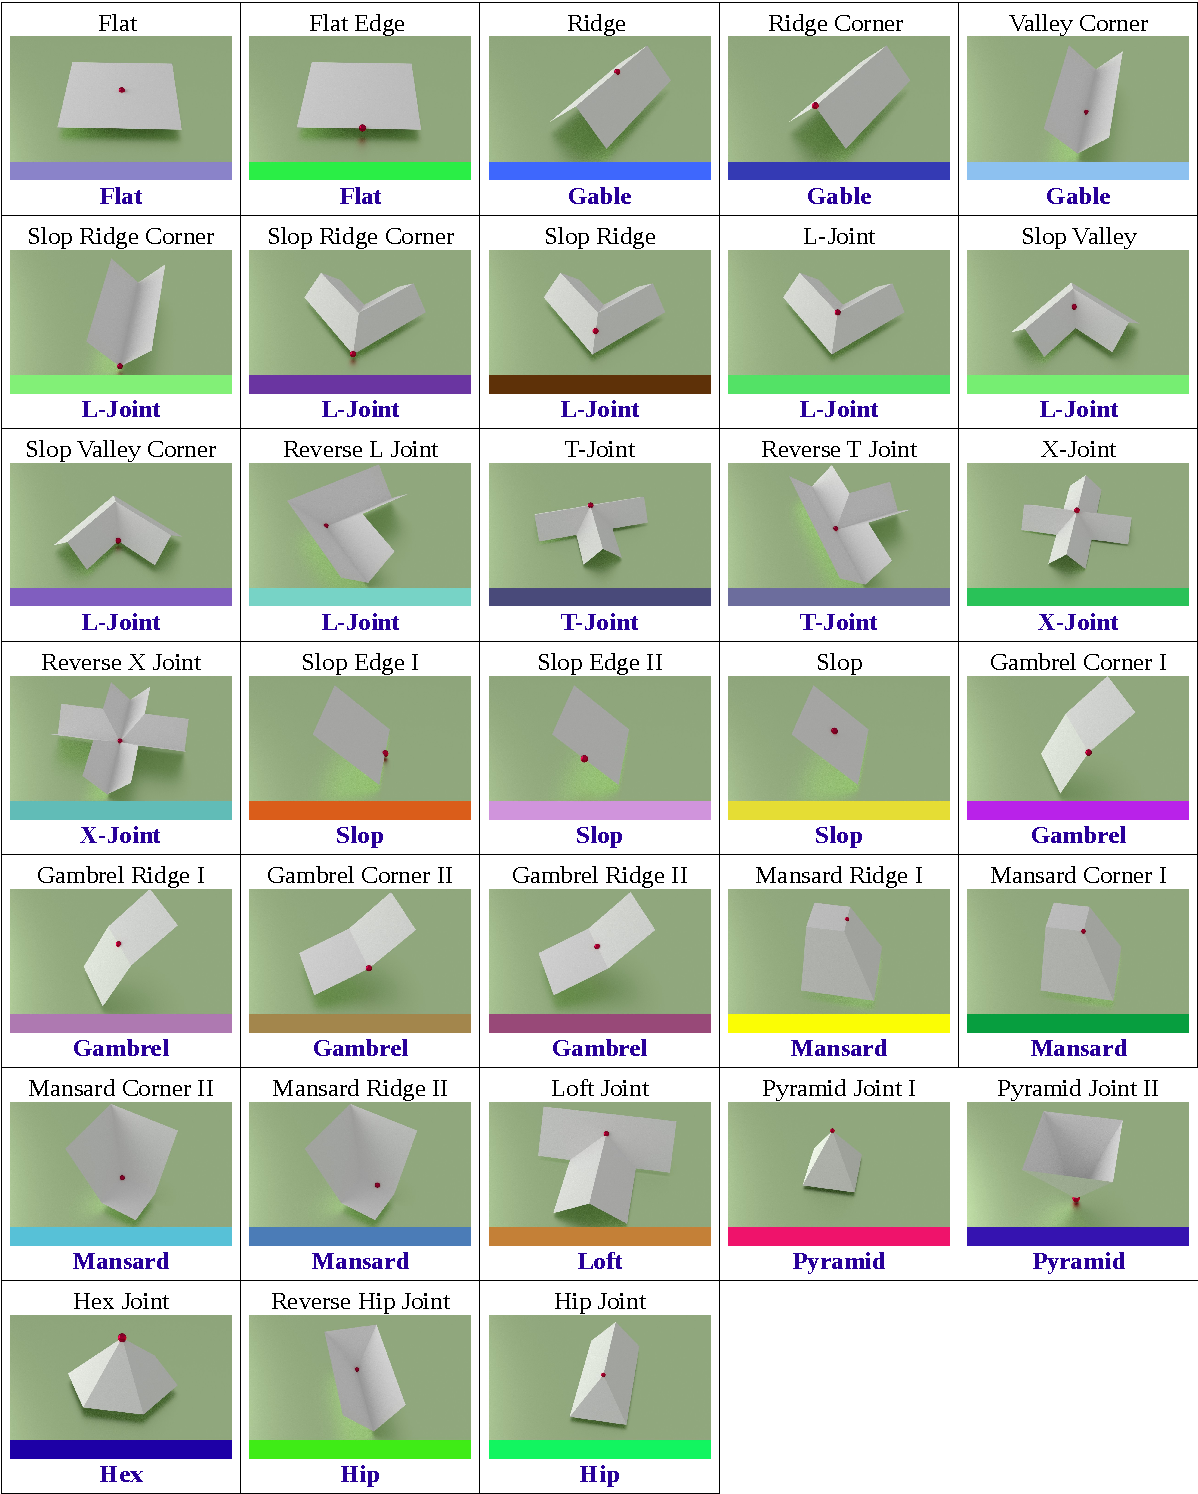
\includegraphics{Pic/PDF/TableOfAllRoofTypes2.pdf}}}
\end{tabular}}
\caption{Illustration of all semantic points used in my work, red sphere on each roof represent the typical location of semantic point, the color bar under each image correspond to all color labels used in previous demo.}
\label{fig: All Semantic Points}
\end{figure} 

As can be observed in Figure \ref{fig: All Semantic Points}, some roof styles shown in Figure \ref{fig: baseroofs} are used to produce multiple key points. The synthetic variants of the codes are derived from these based models in two ways. First, I generate roof models by changing the parameters of the roofs including height, width and slope. Since it is inaccurate and unreasonable to assume any distribution for these parameters and I want to generate models that can cover as much as possible cases in real world, I evenly draw these parameters from their given ranges. I present the size derivation of each base roof in below:

{\noindent \textbf{Flat:}} A little slop is allowed in my flat roof, so I change the angle between flat surface and ground plane from 0 degree to 10 degree, as an exception, distribution of roofs in between these two angles are even.
\\ \textbf{Gable:} The opening width of gable roof is set to be 10 meters, I change two parameters for gable. Firstly, the median ridge is shifted, starting from center location and end at 2.5 meters from center. Secondly, by fixing opening width, the dihedral angle between slop surface and ground is changed from 20 degree to 75 degree, where mean is 30 degree.
\\ \textbf{Hip:} In addition to how I derive from gable roof, the angle between side slop surface and ground plane is changed from 20 degree to 75 degree where mean is 30 degree.
\\ \textbf{L-Joint:} For each of two branches, derivation of gable is applied.
\\ \textbf{T-Joint:} For each of two branches(vertical and horizontal), derivation of gable is applied.
\\ \textbf{X-Joint:} For each of two branches which cross with each other, derivation of gable is applied.
\\ \textbf{Gambrel:} For two slop surface, the angle between surface tangent direction and z direction is changed. Suppose the angle of upper surface with z is $a_0$ and angle of lower surface with z is $a_1$. Using 45 degree as mean, $a_0$ and $a_1$ are changed from 20 to 75 degree, subject to $a_0-a_1\geq 20$ degree.
\\ \textbf{Hex:} Synchronously change the slop angle of side face from 20 degree to 75 degree, where mean is 30 degree.
\\ \textbf{Mansard:} Synchronously change the slop angle of two side face from 20 degree to 75 degree using 30 degree as mean.
\\ \textbf{Pyramid:} Similar to Hex
\\ \textbf{Shed:} Change slop angle from 20 degree to 75 degree using 30 degree as mean.
\\ \textbf{Loft:} For slop surface, Change slop angle from 20 degree to 75 degree using 30 degree as mean and for gable part, please refer to derivation of gable.

In addition to size variation, I also consider erosions of roofs, because it is common in my data to have eroded roofs due to unknown reasons. Four versions with different magnitude of erosion are derived using approach described in \cite{GG07} for each generated roof which are shown in Figure.

\begin{figure}[h]
\centerline{
\begin{tabular}{c}
  \resizebox{0.8\textwidth}{!}{\rotatebox{0}{
  \includegraphics{Pic/PDF/deform2.pdf}}}
\end{tabular}}
\caption{Illustration of erosion in my data. Three different levels of filtering are applied to each roof. In total, including original version, four versions are used in my work.}
\label{fig: All Semantic Points}
\end{figure} 

\clearpage

\Chapter{Learning From Synthetic Data} \label{chapter: learning from synthetic data}

\Section{Introduction} \label{Learn: introduction}

Directly use and learn synthetic data will most likely cause a failure or performance going downward in machine learning even the amount of synthetic data is far enough. Because, synthetic data is generated using parametric model which is a simplification of actual data. Thus, intrinsic patterns and noises owned by actual data do not appear in synthetic data. An example of actual roof edge image and corresponding synthetic roof edge image in my work \cite{ZX14} is shown in Figure \ref{fig: realandsynthetic}. It could be seen from the figure that synthetic building roof image characterize the primary structure only which is a boundary of hexagon. However, the actual roof image in real world comes with more edges extract from inside and edges extracted from other buildings outside the boundary. Some times, such differences could be caused by method of data collection itself, such as a the dataset I used in my work \cite{ZX:14}, that it is very hard for synthetic data to compensate these difference which is not necessary either. Actually, it is almost impossible to simulate every possible noise or inherent patterns in synthetic data using parametric model, which is not the intention of creation of parametric models in my method.   

\begin{figure}[htb]
\centerline{
\begin{tabular}{cc}
  \resizebox{0.2\textwidth}{!}{\rotatebox{0}{
  \includegraphics{Pic/PDF/ChamferMatching/boundEdgeMask.pdf}}}
  &
  \resizebox{0.2\textwidth}{!}{\rotatebox{0}{
  \includegraphics{Pic/PDF/ChamferMatching/buildingEdgeImage.pdf}}}
  \\
  Actual & Synthetic
\end{tabular}}
\caption{An example of actual roof edge image and corresponding synthetic roof edge image in my work \cite{ZX14} is shown in above figures.}
\label{fig: realandsynthetic}
\end{figure} 

Such differences between actual data and synthetic data is very hard to eliminate in data space and will cause a shift of synthetic data domain from actual data domain. Thus any machine learning framework learned from these synthetic data will most likely failed to work for actual data. Such shift is defined as a \textit{Synthetic Gap} in my work \cite{Zhang2014Autoencoder} which will be discussed in detail in Chapter \ref{chapter: synthetic gap}. It is necessary for a learning procedure to remove or at least weaken such discrepancy in order to have a successful recognition result later on.

%In my researches, features are designed and extracted to weaken or even eliminate such discrepancy. Features of two purpose are used in my research. First, features are designed to capture the common characteristics of both actual and synthetic data. Features of this category will focus on the most evident and common characteristics of both data, thus they ignore the additional information of actual data and less sensitive to patterns and noises existing in actual data only. In second category, features are extracted to compensate additional information for synthetic data. In other words, I try to learn the extra patterns of actual data and evolve these information in features used to describe synthetic data.

Information contained by actual data and synthetic data is not equivalent. Actual data could either contains more information in terms of noises and inherent patterns, or contain less information due to data loss such as occlusion in images. Synthetic data used in my work are created based on several parametric prototypes. The prototypes are composed of and simplified to contain the most basic and essential structure of actual data. 

A general goal of feature extraction is to minimize the difference between actual data and synthetic data in extracted features. There two ways to achieve such goal First, extracted features has to be able to catch the most essential characteristics between actual data and synthetic data, thus ignore all the noises and inherent patterns contained . Second, extracted features should be able to compensate these additional information for synthetic data. Under these two directions, several techniques and algorithms are invented in my works. 

\Section{Related Work} \label{Learn: relatedwork}

Most of existing works create synthetic data as a perturbation of original data \cite{Comput.Sci.&Appl.Math.1997}\cite{Ulanova2014}\cite{2012}\cite{VT:03}\cite{VT:04}\cite{NJ:09}. Synthetic data under this domain is generated by either deforming original data using geometric transformation such as scaling, rotation, slant, shrinking ans so on or degradation model such as adding noise, erosion, removing parts and so on. Such data synthesis is very easy to implement in practise although, results in very limit data coverage in data space. Thus, generated synthetic data still carry the same amount of information and stay in the same disjunct as original data. 

So far as I know, just very a few existing works treat synthetic data specially either in feature extraction or learning procedure. One of earliest works dealing with this problem is \cite{Comput.Sci.&Appl.Math.1997}. In this work, authors pioneer to use synthetic data in character recognition. They assume characters undergo a series of geometric transformation defined by them. To simulate real data, their recognizer is trained using synthetic data using their transformation. An interesting setup in their procedure is they apply a set of predefined inverse perturbations to the input image and are expected to include the true perturbation that actually made the input image different from its standard pattern. The corresponding inverse image will be very close the original standard pattern and could be easily recognized by some known method if an inverse perturbation actually corresponds to the true perturbation. Therefore in their learning pipeline, each inverse image is submitted separately to a conventional recognition system, the output score of which is then compared to others. It is clear that among the scores, the one corresponding to the true perturbation can be expected best. Since each score is attached to a class, the recognition scheme is in fact a by-product of the reversing process. A demonstration of this system is show in Figure \ref{fig: inverseperturbation}. Similar ideas are implemented in \cite{2012} and \cite{Zhang2012} in which degradation model or transformation model are trained and tested separately.

 \begin{figure}[h]
\centerline{
\begin{tabular}{c}
  \resizebox{0.6\textwidth}{!}{\rotatebox{0}{
  \includegraphics{Pic/PDF/inverseperturbationslearning.pdf}}}
\end{tabular}}
\caption{The schema of perturbation-based recognition of \cite{Comput.Sci.&Appl.Math.1997} is shown above.}
\label{fig: inverseperturbation}
\end{figure}   

Another strategy to handle the inherent difference between synthetic data and actual data is to use highly abstract features which to some extent could ignore divergence between two data and are able to extract the most common and essential characteristics from the two data. I notice such idea is applied in \cite{Ulanova2014} where to build a optical character recognition (OCR) system, a Kolmogorov complexity distance is used to measure the similarity between two data. Kolmogorov complexity measures the amount of information contained by each data which is done by computing the highest compression ratio of data when being compressed. By using this feature, feature extraction process ignore the concrete differences between data and focus on most essential information contained in the data.
  

Most of existing works generate synthetic data in feature space. Most of techniques are invented to generate and learn synthetic data in feature space. I put the discussion of using synthetic data in feature space to Chapter \ref{chapter: feature space} and use that chapter to present more details of algorithms and strategies.  

\Section{Features to Ignore Additional Information in Actual Data}

\Subsection{Roof Style Classification} In my work \cite{AndiZang2015}, my goal is to classify actual satellite roof edge images using synthetic edge images I created in Chapter \ref{chapter: data space}. The synthetic data is created as connected line segments on image to represent roof main structures such as ridge and valleys. In actual roof edge images, due to low image quality in original source images and noises coming from for example shadows, occlusions and small objects on roofs, the edges representing main roof structures are composed of intermittent short segments and a lot of random size circles. Due to these defect, traditional image features such as Histogram of Gradient (HOG), Local Binary Pattern (LBP) do not work very well on minimizing the difference between actual data and synthetic data.

To facilitate a better learning from synthetic satellite roof edge images, I propose a new image feature called Histogram of Oriented Rays (HOR). HOR works by tracing the longest continuous ray in each direction centerred at each pixel. A few parameters are set to enable HOR to be tolerant to small gaps along the ray and a small range of perturbation of the pixels on the ray. Similar to HOG feature, HOR uses a histogram to save information from all orientations around a pixel, shown in Figure \ref{fig: HOR}. The exact algorithm of HOR is given in Algorithm 

\begin{figure}[h]
	\centerline{
		\begin{tabular}{cc}
			\resizebox{0.3\textwidth}{!}{\rotatebox{0}{
					\includegraphics{Pic/PDF/andi/figure9a.pdf}}}
			&
			\resizebox{0.22\textwidth}{!}{\rotatebox{0}{
					\includegraphics{Pic/PDF/andi/figure9bpdfpages.pdf}}}
			\\
		\end{tabular}}
		\caption{Illustration of HOR feature.}
		\label{fig: HOR}
\end{figure}

{\linespread{1.5}
\begin{algorithm}[htb]   
	\caption{ Histogram of Rays}   
	\label{alg: 2}   
	\begin{algorithmic}[1] 
		\REQUIRE ~~\\
		Given point $p$ on gray scale image $I$;\\
		Number of search orientation $D$;\\
		Searching threshold $T$;\\
		Mimimum gap length $G$;\\
		Length of HOR feature vector $L$;
		\ENSURE ~~\\  
		The HOR feature vector $V$ of point $I$; 
		\FOR{$i=1$ \TO $|D|$}
			\STATE Terminator $count = 0$;
			\STATE Calculate pixel list on direction $\frac{D}{2\pi} \Rightarrow IDX$ from $p$;
			\STATE Index $j=0$;
			\WHILE{$count<G$}
				\IF{$IDX_{j+1}/IDX_j < T$}
					\STATE $count ++$;
				\ELSE
					\STATE $count = 0$;
				\ENDIF
				\STATE $j ++$;
			\ENDWHILE
			\STATE $V_i = j$;
		\ENDFOR 
		\STATE Sampling $V$ from length $D$ to $L$;
		\RETURN $V$; 
	\end{algorithmic}  
\end{algorithm} 
}

To evaluate the performance of HOR, a test set containing 1783 roof images including flat, hip, gable and half hip roof styles is tested. I use random forest as a base learner and compare results to features including HOG, Shape Context (SC), LBP and so on. A same feature merging rule is used in all tests that each feature descriptor has 5 pixels per cell, 2 cells per block and 50\% overlapping between blocks. The precision and recall obtained using HOR feature are show in Table \ref{table: pr}.

\begin{table}[t]
\caption{Precision and recall of hip (HIP), gable (GBL), flat (FLT) and half hip (HHP) styles classified by Random Forest is shown in above table. I use red font to show highest value among results.}
	\centering
	\scalebox{1.0}
	{
		\begin{tabular}{ccccc}
			\hline \hline
			&\multicolumn{2}{c}{{Real Roof}} & \multicolumn{2}{c}{{Combination}}\\ 
			\hline
			
			&\multicolumn{1}{c}{{Precision}} & \multicolumn{1}{c}{{Recall}} & \multicolumn{1}{c}{{Precision}} & \multicolumn{1}{c}{{Recall}}\\

			
			HIP & 0.953 & 0.823 & 0.963 & 0.814 \\

			
			GBL & 0.877 & 0.901 & 0.886 & 0.882 \\

			
			FLT & 0.784 & 0.977 & 0.745 & 0.959 \\

			
			HHP & 0.893 & 0.439 & 0.967 & 0.509 \\ 			 
			\hline
			
		\end{tabular}
	}
	\label{table: pr}
\end{table}

I show the accuracies of each feature using my testing data classified by the classifier, which trained by the combination of my training
dataset and synthetic models. The accuracies is presented in Table \ref{table: ac}. The precisions calculated by using HOR and HOG combination for hip, gable, flat and half hip(93.1\%, 95.5\%, 98.2\% and 66.7\%) shows a better result than using HOR(89.8\%, 95.0\%, 96.8\% and 63.2\%) and HOG(80.5\%, 88.2\%, 95.4\% and 59.7\%) separately. The results show that for current edge detection approach and training method, HOR alone, or HOR combined with HOG, are considered to be more appropriate as the input feature for roof style recognition system.

\begin{table}[t]
\caption{The comparison of accuracies between HoG (HOG), Shape Context (SC), HoR (HOR) and their combinations by running Random Forest  approach.}
	\centering
	\scalebox{1.0}
	{
		\begin{tabular}{lcccc}
			\hline \hline
			
			&HIP & GABLE & FLAT & HALFHIP\\
			\hline
			
			HOG & 0.805 & 0.882 & 0.954 & 0.597 \\
			
			SC & 0.350 & 0.828 & 0.959 & 0.140 \\
			
			HOR & 0.898 & 0.950 & 0.968 & 0.632 \\
			
			LBP & 0.000 & 0.986 & 0.631 & 0.000 \\
			
			HOR+HOG & 0.931 & 0.959 & 0.982 & 0.667 \\
			
			HOR+SC & 0.619 & 0.891 & 0.959 & 0.436 \\
			
			HOG+SC & 0.752 & 0.959 & 0.945 & 0.474 \\
			
			SC & 0.743 & 0.869 & 0.963 & 0.509 \\
			\hline
		\end{tabular}
	}
	\label{table: ac}
\end{table}

There is no roof labelled as half hip in the subset weevaluate of my sponsors dataset. The only one I obtain is in Figure 1, where captured in Stanford campus. I can’t say the accuracy for half hip style is 100\% based on this ideal same. The final accuracy of roof in complex footprint recognition is 95.2\%, 84.6\% and 91.7\% for flat, hip and gable styles.

\Subsection{Satellite Building Image Retrieval} An extension of classic chamfer matching algorithm is proposed in my another work \cite{ZX14}. In this work, I deal with a image retrieval problem for edge images extracted from building roof top. Different from roof top images I used in other works, roof top images in \cite{ZX14} are extracted from artificial building footprint, thus, the edge images contain only boundaries of a roof. An example of target roof image and synthetic roof image is given in \ref{fig: realandsynthetic}.

The task in this work is to retrieve the most matching actual roof edge image given a synthetic roof edge image. Challenges come from different aspects. First, actual edge image are generated by extracting edges from satellite images, thus edge images could contain a great number of edges from other unrelated objects in image. In addition, due to lighting condition, buildings in image could either be too dim or shadowed by dark areas. Second, synthetic edge image basically are polygons representing the boundary of a building. These polygons give a very approximate shape about an actual building, thus, the polygon could be very different from the actual building roof top.

In order to be resistant to all kinds of defects in actual roof edge images, I extend the classic chamfer matching feature and design a new chamfer matching that is much more robust when facing an image retrieval problem such us the one in my work.

The idea of using Chamfer matching for image registration was first introduced by Barrow \textit{et al.} \cite{HB:77} where they try to find the model of a coastline in a segmented satellite image. Since then many variations of the Chamfer matching have been introduced.

An important variation of the Chamfer matching by Borgefors \cite{GB:88} uses a hierarchical Chamfer matching algorithm (HCMA). This algorithm uses an image pyramid in searching for the optimal position of a template. The search for an optimal position is made in different resolution levels of the pyramid by using a representation of the distance image. The optimization of the objective function is done by discretizing the transformation parameters and stepping through them in each pyramid level. The speed of HCMA can be improved by modifying the computation of the distance transform image and by selecting the starting search position \cite{QZ:09}. An HCMA algorithm based on interesting points has been used in \cite{JY:95} where a parallel computation scheme of Chamfer matching is discussed. The selection of interesting points in this work is done through a dynamic threshold scheme guided by a histogram.

A Chamfer matching algorithm which is based on multiple features was introduced by Gavrila et al.\cite{DG:98},\cite{DG:99}, where it is proposed to use edge orientation as a feature. An orientation channel is created for each feature and a distance transform image is generated for edges in the channel. This method uses a hierarchical scheme for matching multiple templates with an image in which similar templates are grouped at different levels.

Shotton et al.\cite{JS:08} use the Chamfer distance with an additional cost which measures the mismatch of edge orientations given by the average difference in orientation between template edges and the closest edges in target image. Instead of explicitly formulating a separate term of orientation mismatch, the orientation difference is generalized in the computation of the Chamfer distance\cite{ML:10}. A comparison between shape context matching and Chamfer matching is conducted in \cite{AT:03}, where results show that using the Chamfer matching is faster than matching using shape context and that global matching using Chamfer matching is better than using shape context.

\Subsection{Chamfer Matching} Let $U$ and $V$ be two binary edge images, where $U$ is the target image and $V$ is the template image. Let $\{u_j\}_{j=1}^m$ and $\{v_i\}_{i=1}^n$ be the edge pixels in these images respectively. Let $U(u_j)$ denote the value of image $U$ at location $u_j$.

In chamfer matching, I seek a correspondence between $\{u_j\}$ and $\{v_i\}$ under transformation $W$. Assuming that the transformation $W$ between the template and target images is rigid with translation $T$ and rotation $R$, a template edge pixel $v_i$ is transformed into the target image by using following expression:
\begin{equation}
W(v_i;R, T)=R \cdot v_i + T \equiv v_i^{\scalebox{.5}{\textit{U}}}
\end{equation}
Given a distance metric $d(\cdot)$, I can solve for the transformation parameters $T$ and $R$ by minimizing the total distance:
\begin{equation}
D(U, V;R, T)=\frac{1}{n}\sum_{1\leq i\leq n}d(v_i^{\scalebox{.5}{\textit{U}}}, u_j)
\label{Equ: Dist between U and V}
\end{equation}
where $u_j$ is the closest target edge pixel to $v_i^{\scalebox{.5}{\textit{U}}}$ in the sense of the distance metric $d(\cdot)$.

The computation of $d(v_i^{\scalebox{.5}{\textit{U}}}, u_j)$ can be done in linear time using the \textit{distance transform} of the target image\cite{AR:66}. Denoting the distance transform image of $U$ by $U_{\mathcal{DT}}$, I can write Equation (\ref{Equ: Dist between U and V}) as:

\begin{equation}
D(U, V;R, T)=\frac{1}{n}\sum_{1\leq i\leq n}U_{\mathcal{DT}}(v_i^{\scalebox{.5}{\textit{U}}}).
\label{Equ: Dist between U and V 2}
\end{equation}

Various types of distance transforms can be produced using different distance metrics $d(\cdot)$. In \cite{AR:66}, city-block distances are used and a two-step linear algorithm is proposed to compute the distances. Euclidean distances approximations are provided by Borgefors\cite{GB:86}, Montanari\cite{UM:68}, and Danielsson\cite{PD:80}. An efficient squared Euclidean distance computation algorithm is described by Felzenszwalb\cite{PF:04}, Felzenszwalb's algorithm can be generalized to compute other distances. 

\Subsection{Extended Chamfer Matching} I extend the Chamfer matching in several ways. First, I extend the basic Chamfer matching and obtain additional robustness by jointly minimizing the spatial distance between pixels and the misalignment of edge orientations. A similar distance metric is used in \cite{ML:10} where a linear representation of edges is generated to model the edge orientation. The proposed approach avoids the need for a linear representation of edges by computing the edge orientation directly from the images.

\begin{figure}[h]
\centerline{
\begin{tabular}{cc}
  \resizebox{0.87\textwidth}{!}{\rotatebox{0}{
  \includegraphics{Pic/PDF/ChamferMatching/Screenshot_EdgeDirection_1.pdf}}}
\end{tabular}}
\caption{Computing edge orientation in the binary template image.}
\label{fig: edge direction}
\end{figure}

The edge orientation at each location is computed as a vector perpendicular to the gradient vector at that location. In the target image, the distance transform image $U_{\mathcal{DT}}$ is used to compute the edge orientation at each location. Specifically, given a transformed location $v_i^{\scalebox{.5}{\textit{U}}}$, its edge orientation $\vec{v}_i^{\scalebox{.5}{\textit{U}}}$ is computed as a vector perpendicular to the gradient vector $\nabla{U_{\mathcal{DT}}(v_i^{\scalebox{.5}{\textit{U}}})}$. To compute the edge orientation in the binary template image $V$, I create a gradient vector field around edges by smoothing $V$ using a standard Gaussian kernel. The edge orientation vectors $\vec{v_i}$ are then calculated as vectors perpendicular to the gradient vectors obtained from the gradient vector field. An example of the edge orientation computation in $V$ is shown in Figure \ref{fig: edge direction}.

Having the edge orientation computed in both the target and template images, the distance between pixels ${v}_i^{\scalebox{.5}{\textit{U}}}$ and $u_j$ is computed by:

\begin{equation}
d(v_i^{\scalebox{.5}{\textit{U}}}, u_j)=\lambda U_{\mathcal{DT}}(v_i^{\scalebox{.5}{\textit{U}}}) + (1-\lambda)(1- \|\cos(\alpha_{v_i^{\scalebox{.5}{\textit{U}}}})\|)
\label{Equ: distance metric}
\end{equation}

where $\lambda$ is a weight factor that controls the importance of orientation mismatch, $\cos(\alpha_{v_i^{\scalebox{.5}{\textit{U}}}})=\langle{\vec{v}_i^{\scalebox{.5}{\textit{U}}}}, \vec{v_i} \rangle$ measures the orientation mismatch, and it is assumed that $\vec{v}_i^{\scalebox{.5}{\textit{U}}}$ and $\vec{v_i}$ are normalized.

A squared Euclidean norm is used in the first term of Equation (\ref{Equ: distance metric}), which gives a larger penalty to mismatched pixels. A method to generate the squared Euclidean norm distance transform in linear time is described in \cite{PF:04}.

\Subsection{Edge Distance Variance} To have a robust matching result, the matching error of a pixel $v_i$ should not solely depend on $d(v_i^{\scalebox{.5}{\textit{U}}}, u_j)$. This is because it is possible that $v_i^{\scalebox{.5}{\textit{U}}}$ will be an incorrect edge pixel in the target image that happened to have a small error. Based on this consideration, I argue that to get a confident measurement of the matching error it is necessary to take into account the matching error of neighbouring pixels.

\begin{figure}
\centerline{
\begin{tabular}{c} % obj 1 24192177 81%
  \resizebox{0.9\textwidth}{!}{\rotatebox{0}{
  \includegraphics{Pic/PDF/ChamferMatching/Good_Good.pdf}}}
  \\
  (a) Modified distance\;=\;1.5 $\times$ 0.55\;=\;0.82
  \\
  \resizebox{0.9\textwidth}{!}{\rotatebox{0}{
  \includegraphics{Pic/PDF/ChamferMatching/Good_Bad.pdf}}}
  \\
  (b) Modified distance\;=\;1.5 $\times$ 2.54\;=\;3.82
  \\
\end{tabular}}
\caption{Example of the modified distance measure. In both cases I use a neighborhood of size $p=13$, and select the lowest $q=5$ neighbors. While the distance at the pixel is the same (1.5), the modified distance measure in the bottom example is higher due to the larger distance to neighbors.}
\label{fig: modified distance.}
\end{figure} 

Given the transformed template edge pixels $\{v_i^{\scalebox{.5}{\textit{U}}}\}_{i=1}^n$, I find for each pixel $v_i^{\scalebox{.5}{\textit{U}}}$ matching scores for the $p$ closest transformed template edge pixels. To estimate contextual matching error of $d(v_i^{\scalebox{.5}{\textit{U}}}, u_j)$ at location $v_i^{\scalebox{.5}{\textit{U}}}$, the $q$ pixels with lowest matching error, where $q<p$, are selected. I denoted these $q$ pixels as $\{v_k^{\scalebox{.5}{\textit{U}}}\}_{k=1}^q$. I then calculate the variance of the distance $d(v_i^{\scalebox{.5}{\textit{U}}}, u_j)$ of the $q$ selected pixels:$\varphi(v_i^{\scalebox{.5}{\textit{U}}})=\frac{1}{q}\sum_{k=1}^q (d(v_k^{\scalebox{.5}{\textit{U}}}, u_j)-\bar{d})^2$, where $\bar{d}$ is the average matching error of the $q$ neighbors.

The distance variance $\varphi(v_i^{\scalebox{.5}{\textit{U}}})$ provides a more stable assessment of the matching result at $v_i$. The parameters $p$ and $q$ control the size of the contextual information used in the computation. A larger $p$ leads to more contextual information included while $q$ helps in excluding outliers. In my experiments, I set $p=13$ and $q=5$. Since $p$ and $q$ are constants, the asymptotic time complexity of the algorithm is not affected by them. From a practical point of view, to save time when searching for the $p$ closest neighbors at each $v_i$, I generate and maintain a list of $p$ closest neighbors for each $v_i$ before the matching begins. 

As I would like to give preference to distance measures with small distance variance, I modify the distance metric in Equation (\ref{Equ: distance metric}) by multiplying it by a factor which is proportional to the distance variance:

\begin{equation}
d_{\varphi}(v_i^{\scalebox{.5}{\textit{U}}}, u_j)=d(v_i^{\scalebox{.5}{\textit{U}}}, u_j)\times(1+\varphi(v_i^{\scalebox{.5}{\textit{U}}}))
\label{equ: distance variance}
\end{equation}  

Figure \ref{fig: modified distance.} shows an example of the modified distance computation.

The significance of multiplying the distance variance in Equation (\ref{equ: distance variance}) lies in several aspects. First, the distance measure is no longer solely dependent on each pixel's individual matching distance as the distance now considers the relationship between a pixel and its best matched neighbours. Consequently, I expect each pixel and its connected neighbours to have a small distance. Second, the variance in Equation (\ref{equ: distance variance}) makes it much easier to separate well matched pixels from mismatched ones by increasing the width of boundary that separates the well matched pixels and mismatched ones.

I tested the proposed approach on two datasets, where each contains 1000 building models selected from a San Francisco (SF) and a Chicago (CHI) urban area.

\begin{figure}
\centerline{
\begin{tabular}{ccccc} % obj 1 24192177 81%
  \resizebox{0.16\textwidth}{!}{\rotatebox{0}{
  \includegraphics{Pic/PDF/ChamferMatching/shadowed/SF/SearRegionEdge/searchAreaEdge_24192177.pdf}}}
  &
  \resizebox{0.16\textwidth}{!}{\rotatebox{0}{
  \includegraphics{Pic/PDF/ChamferMatching/shadowed/SF/CMMatched/24192177.pdf}}}
  &
  \resizebox{0.16\textwidth}{!}{\rotatebox{0}{
  \includegraphics{Pic/PDF/ChamferMatching/shadowed/SF/BadMatched/24192177.pdf}}}
  &
  \resizebox{0.16\textwidth}{!}{\rotatebox{0}{
  \includegraphics{Pic/PDF/ChamferMatching/shadowed/SF/GoodMatched/24192177.pdf}}}
  &
  \resizebox{0.12\textwidth}{!}{\rotatebox{0}{
  \includegraphics{Pic/PDF/ChamferMatching/shadowed/SF/ResultImage/bw_24192177.pdf}}}
  \\ \\% obj 2 24193136 56%
  \resizebox{0.16\textwidth}{!}{\rotatebox{0}{
  \includegraphics{Pic/PDF/ChamferMatching/shadowed/SF/SearRegionEdge/searchAreaEdge_24193136.pdf}}}
  &
  \resizebox{0.16\textwidth}{!}{\rotatebox{0}{
  \includegraphics{Pic/PDF/ChamferMatching/shadowed/SF/CMMatched/24193136.pdf}}}
  &
  \resizebox{0.16\textwidth}{!}{\rotatebox{0}{
  \includegraphics{Pic/PDF/ChamferMatching/shadowed/SF/BadMatched/24193136.pdf}}}
  &
  \resizebox{0.16\textwidth}{!}{\rotatebox{0}{
  \includegraphics{Pic/PDF/ChamferMatching/shadowed/SF/GoodMatched/24193136.pdf}}}
  &
  \resizebox{0.12\textwidth}{!}{\rotatebox{0}{
  \includegraphics{Pic/PDF/ChamferMatching/shadowed/SF/ResultImage/bw_24193136}}}
  \\ \\% obj 3 24194350 66%
  \resizebox{0.16\textwidth}{!}{\rotatebox{0}{
  \includegraphics{Pic/PDF/ChamferMatching/shadowed/SF/SearRegionEdge/searchAreaEdge_24194350.pdf}}}
  &
  \resizebox{0.16\textwidth}{!}{\rotatebox{0}{
  \includegraphics{Pic/PDF/ChamferMatching/shadowed/SF/CMMatched/24194350.pdf}}}
  &
  \resizebox{0.16\textwidth}{!}{\rotatebox{0}{
  \includegraphics{Pic/PDF/ChamferMatching/shadowed/SF/BadMatched/24194350.pdf}}}
  &
  \resizebox{0.16\textwidth}{!}{\rotatebox{0}{
  \includegraphics{Pic/PDF/ChamferMatching/shadowed/SF/GoodMatched/24194350.pdf}}}
  &
  \resizebox{0.12\textwidth}{!}{\rotatebox{0}{
  \includegraphics{Pic/PDF/ChamferMatching/shadowed/SF/ResultImage/bw_24194350.pdf}}}
  \\ \\% obj 5 24362707 54%
  \resizebox{0.16\textwidth}{!}{\rotatebox{0}{
  \includegraphics{Pic/PDF/ChamferMatching/shadowed/SF/SearRegionEdge/searchAreaEdge_24362707.pdf}}}
  &
  \resizebox{0.16\textwidth}{!}{\rotatebox{0}{
  \includegraphics{Pic/PDF/ChamferMatching/shadowed/SF/CMMatched/24362707.pdf}}}
  &
  \resizebox{0.16\textwidth}{!}{\rotatebox{0}{
  \includegraphics{Pic/PDF/ChamferMatching/shadowed/SF/BadMatched/24362707.pdf}}}
  &
  \resizebox{0.16\textwidth}{!}{\rotatebox{0}{
  \includegraphics{Pic/PDF/ChamferMatching/shadowed/SF/GoodMatched/24362707.pdf}}}
  &
  \resizebox{0.12\textwidth}{!}{\rotatebox{0}{
  \includegraphics{Pic/PDF/ChamferMatching/shadowed/SF/ResultImage/bw_24362707.pdf}}}
  \\ \\% obj 4 24204619 72%
  \resizebox{0.16\textwidth}{!}{\rotatebox{0}{
  \includegraphics{Pic/PDF/ChamferMatching/shadowed/SF/SearRegionEdge/searchAreaEdge_24204619.pdf}}}
  &
  \resizebox{0.16\textwidth}{!}{\rotatebox{0}{
  \includegraphics{Pic/PDF/ChamferMatching/shadowed/SF/CMMatched/24204619.pdf}}}
  &
  \resizebox{0.16\textwidth}{!}{\rotatebox{0}{
  \includegraphics{Pic/PDF/ChamferMatching/shadowed/SF/BadMatched/24204619.pdf}}}
  &
  \resizebox{0.16\textwidth}{!}{\rotatebox{0}{
  \includegraphics{Pic/PDF/ChamferMatching/shadowed/SF/GoodMatched/24204619.pdf}}}
  &
  \resizebox{0.12\textwidth}{!}{\rotatebox{0}{
  \includegraphics{Pic/PDF/ChamferMatching/shadowed/SF/ResultImage/bw_24204619.pdf}}}
  \\
  (a) & (b) & (c) & (d) & (e)
\end{tabular}}
\caption{Results of matching partially occluded buildings. (a) Edge images detected from target image. (b)-(d) Results of the CM algorithm, the results of the DCM algorithm and the results of the proposed algorithm, respectively. (e) The pixels selected for computing the average error during the matching process.}
\label{fig: incomplete building results}
\end{figure} 

The four parameters in Algorithm \ref{alg:D} are set as follows: $\theta=50\%$, $t_s=5$, $t_{\alpha}=15$, and $t_{\varphi}=0.8$. By setting these parameters, I allow for at least $50\%$ of template pixels to be inliers in the computation of $D(U, V;R, T)$; the accepted matching error of obtained transformation has to be within error of $5$ pixels in terms of spatial distance and $15$ degrees in terms of orientation difference; finally $0.8$ average distance variance is used to rule out outliers during Chamfer matching.

In my experiments, I test the accuracy of my algorithm in estimating the optimal transformation during alignment. I manually labelled the ground truth locations of the building roofs in satellite images. The accuracy of the result is measured by the ratio of overlap between the bounding box of the ground truth roof mask and the one transformed by the proposed algorithm. Note that simply measuring the Root Mean Square error (RMS) between the aligned targets and templates is not accurate as it  is sensitive to broken edges and incorrect alignments.

\begin{figure}
\centerline{
\begin{tabular}{c}
\begin{tabular}{cc}
  \resizebox{0.5\textwidth}{!}{\rotatebox{0}{
  \includegraphics{Pic/PDF/ChamferMatching/MeanCoverageComparison_SF.pdf}}}
  &
  \resizebox{0.5\textwidth}{!}{\rotatebox{0}{
  \includegraphics{Pic/PDF/ChamferMatching/CoverageComparison_SF.pdf}}}
\end{tabular}
\\
  San Francisco
\\
\begin{tabular}{cc}  
  \resizebox{0.5\textwidth}{!}{\rotatebox{0}{
  \includegraphics{Pic/PDF/ChamferMatching/MeanCoverageComparison_Chicago.pdf}}}
  &
  \resizebox{0.5\textwidth}{!}{\rotatebox{0}{
  \includegraphics{Pic/PDF/ChamferMatching/CoverageComparison_Chicago.pdf}}}
\end{tabular}
\\ 
  Chicago
\end{tabular}}
\caption{Experimental evaluation results on the San Francisco (upper row) and Chicago (lower row) datasets. The left and right columns show different evaluation metrics.}
\label{fig: result comparison}
\end{figure}

I first test the proposed Chamfer matching without using global constraint. I divide my evaluation into two parts. In the first part, the evaluation is done on all the buildings of both datasets using the same $\lambda$. I then change $\lambda$ between $0$ and $1$ to compare the robustness of the proposed approach, and evaluate the relative importance of the spatial and angular terms. In the second part, to assess the performance of the proposed algorithm on matching occluded objects, I specifically run tests on building images in which the target buildings are partially occluded. In all the tests, I compare my results with that of the directional Chamfer matching (DCM) proposed in \cite{ML:10} and the basic Chamfer matching (CM). Note that the result of CM is a special case of the DCM algorithm when $\lambda=1.0$.

Two kinds of metrics were used in my evaluation. In the first metric, I compute the average ratio of overlap area in the two datasets. In the second metric, I consider only results with area overlap above a certain rate ($85\%$ and $90\%$). 

In the first test where all the buildings were included, it could be observe in Figure \ref{fig: result comparison} that my algorithm generates better results compared with DCM and CM at almost every setting of $\lambda$. In both datasets, my algorithm maintains a similar and consistent performance, while DCM performs differently on the two datasets.

%\begin{table}[h]
%\centering
%\scalebox{1}
%{
%\begin{tabular}{cc|c|c|c|c}
%\cline{3-5}
%& & \tabincell{c}{Metric One } & \tabincell{c}{Metric Two \\ $\geq$ 85\%} & \tabincell{c}{Metric Two \\ $\geq$ 90\%} &\\ 
%\cline{1-5}
%\multicolumn{1}{ |c }{\multirow{2}{*}{\tabincell{c}{SF \\53 Buildings}} } &
%
%\multicolumn{1}{ |c| }{\tabincell{c}{Proposed}} & 91\% & 0.94 & 0.90 &     \\ 
%\cline{2-5}
%\multicolumn{1}{ |c  }{}                             &
%\multicolumn{1}{ |c| }{\tabincell{c}{DCM}} & 63\% & 0.33 & 0.28 &     \\ 
%\cline{2-5}
%\multicolumn{1}{ |c  }{}                             &
%\multicolumn{1}{ |c| }{\tabincell{c}{CM}} & 35\% & 0.20 & 0.18 &     \\ 
%\cline{1-5}
%
%\multicolumn{1}{ |c }{\multirow{2}{*}{\tabincell{c}{CHI \\74 Buildings}} } &
%
%\multicolumn{1}{ |c| }{\tabincell{c}{Proposed}} & 80\% & 0.81 & 0.78 &     \\ 
%\cline{2-5}
%\multicolumn{1}{ |c  }{}                             &
%\multicolumn{1}{ |c| }{\tabincell{c}{DCM}} & 51\% & 0.21 & 0.20 &     \\
%\cline{2-5}
%\multicolumn{1}{ |c  }{}                             &
%\multicolumn{1}{ |c| }{\tabincell{c}{CM}} & 32\% & 0.16 & 0.13 &     \\  
%\cline{1-5}
%\end{tabular}
%}
%\caption{Accuracy results.}
%\label{table: building in shadow}
%\end{table}

\begin{table}[h]
\caption{Accuracy results.}
\centering
\scalebox{1}
{
\begin{tabular}{cccccc}
\hline \hline
& & \tabincell{c}{Metric One } & \tabincell{c}{Metric Two \\ $\geq$ 85\%} & \tabincell{c}{Metric Two \\ $\geq$ 90\%} &\\ 
\hline
\multicolumn{1}{ c }{\multirow{2}{*}{\tabincell{c}{SF \\53 Buildings}} } &
\multicolumn{1}{ c }{\tabincell{c}{Proposed}} & 91\% & 0.94 & 0.90 &     \\ 
\multicolumn{1}{ c  }{}                             &
\multicolumn{1}{ c }{\tabincell{c}{DCM}} & 63\% & 0.33 & 0.28 &     \\ 
\multicolumn{1}{ c  }{}                             &
\multicolumn{1}{ c }{\tabincell{c}{CM}} & 35\% & 0.20 & 0.18 &     \\ 
\hline
\multicolumn{1}{ c }{\multirow{2}{*}{\tabincell{c}{CHI \\74 Buildings}} } &
\multicolumn{1}{ c }{\tabincell{c}{Proposed}} & 80\% & 0.81 & 0.78 &     \\ 
\multicolumn{1}{ c  }{}                             &
\multicolumn{1}{ c }{\tabincell{c}{DCM}} & 51\% & 0.21 & 0.20 &     \\
\multicolumn{1}{ c  }{}                             &
\multicolumn{1}{ c }{\tabincell{c}{CM}} & 32\% & 0.16 & 0.13 &     \\  
\cline{1-5}
\end{tabular}
}
\label{table: building in shadow}
\end{table}

To test proposed algorithm's strength in finding matching targets under partial occlusion, I specifically test and evaluate the algorithms' performances on 53 buildings from San Francisco and 74 buildings from Chicago which are significantly occluded by shadows. I use a parameter of $\lambda=0.7$ in this test. The results are shown in Table \ref{table: building in shadow}. As can be observed, the proposed algorithm achieves 80\% accuracy on both datasets compared with about 50\% accuracy when using DCM and 30\% accuracy when using the original Chamfer matching. Some examples of matching incomplete buildings are shown in Figure \ref{fig: incomplete building results}. 

I finally tested the improvement obtained by the global constraint for $\lambda=0.7$.For both data sets, I obtain at least $2\%$ improvement in terms of accuracy. The comparisons of alignment results with and without global constraint alignment are given in Table \ref{table: gc}.

\begin{table}[h]
\caption{Results of alignment using global constraint. The number on the right side of the arrows show the results obtained by alignment using the global constraint.}
\centering
\scalebox{1}
{
\begin{tabular}{cccc}
\hline \hline
& \tabincell{c}{Metric One } & \tabincell{c}{Metric Two \\ $\geq$ 85\%} & \tabincell{c}{Metric Two \\ $\geq$ 90\%} \\ 
\hline
\multicolumn{1}{ c }{{\tabincell{c}{SF}} }  & 89\% $\rightarrow$ 91\% & 88\% $\rightarrow$ 90\% & 78\% $\rightarrow$ 79\%  \\ 
\multicolumn{1}{ c }{{\tabincell{c}{CHI}} } & 89\% $\rightarrow$ 92\% & 89\% $\rightarrow$ 91\% & 83\% $\rightarrow$ 85\%  \\  
\hline
\end{tabular}
}
\label{table: gc}
\end{table}

\Section{Features to Compensate Additional Information}

There are cases when ignoring additional patterns in actual data are very difficult. An typical example is given in my work \cite{ZX:14} where the exact structure of actual data is hard to be recognized thus there is no way under this scenario to find corresponding geometry of synthetic data. Therefore, rather than designing feature to neglect additional patterns on the side of actual data, I am going to learn additional patterns on actual data and design features which are able to encode these information in the computation.

This done from different aspects in \cite{ZX:14}. First, features in this work are designed to characterize spatial and context information of local point.

Spatial features take into account the neighborhood of each point. So the spatial features are powerful to describe geometry characteristics in the point's neighborhood and so assist in producing a distinct characterization of it. Let $p_i$ be a key point. Let $N_i$ be a neighborhood of the point, containing neighbors in a radius of $\mu$ (0.6 meters in my experiments). I denote the spatial features at $p_i$ using $\mathcal{S}_i$.

\noindent \textbf{i.\;Eigen Features (EF).} I compute the eigenvalues: $\lambda_1, \lambda_2, \lambda_3$ of the covariance matrix of neighbors $N_i$ centred at $p_i$. I then add following features for $p_i$: $\lambda_1$, $\lambda_2$, $\lambda_3$, $\lambda_3-\lambda_2$, $\lambda_2-\lambda_1$, $\lambda_1/(\lambda_1+\lambda_2+\lambda_3)$, $\lambda_2/(\lambda_1+\lambda_2+\lambda_3)$, $\lambda_3/(\lambda_1+\lambda_2+\lambda_3)$, yielding 8 features in total. These features capture the non-planarity of points around $p_i$.

\begin{figure}[h]
\centerline{
\begin{tabular}{c}
  \resizebox{0.6\textwidth}{!}{\rotatebox{0}{
  \includegraphics{Pic/PDF/PointCloudRoofClassification/ShapeDistributionPic.pdf}}}
\end{tabular}}
\caption{Illustration of the frame I used in the computation of the shape distribution features.}
\label{fig: ShapeDistribution}
\end{figure} 

\noindent\textbf{ii.\;Point Feature Histogram (PFH).} These are point cloud features based on histogram which are described in \cite{RBR08}. Taking into account computational efficiency, 3 subdivisions of the features range are used in the feature histogram which yield $3^3=27$ features.

\noindent\textbf{iii.\;Shape Distribution Features (SD).} Shape distribution \cite{RO02} measures global geometric properties of an object by representing object features as a probability distribution. Shape distribution is invariant to translation, rotation and scale and is highly informative in matching objects. Using the ideas of shape distribution I construct four features:
%\setlength{\parskip}{0pt}

\noindent \textbf{1) A2:} Measures the angle between two vectors composed by two neighbors $p_j, p_k\in N_i$ and $p_i$, shown as $\angle{p_j p_i p_k}$ in Figure \ref{fig: ShapeDistribution}. A2 feature is computed for all pairs of points chosen from $N_i$.

\noindent \textbf{2) Az:} Measures the angle between the z direction and a vector pointing from $p_i$ to one neighbor $p_k$, shown as $\angle{z p_i p_k}$ in Figure \ref{fig: ShapeDistribution}. All points in $N_i$ are used to compute this feature.

\noindent \textbf{3) D2:} The is the feature D2 as described in \cite{RO02}. It measures the distance between any two neighbors of $p_i$, an example is shown as $\|p_j p_k\|$ in Figure \ref{fig: ShapeDistribution}. D2 is computed for all pairs of points chosen from $N_i$.

\noindent \textbf{4) Dt:} Measures the angle between $p_i$'s tangent plane and a vector pointing from $p_i$ to another neighbor $p_j$, shown as $\angle{p'_j p_i p_j}$ in Figure \ref{fig: ShapeDistribution}, where $p'_j$ is the projection of $p_j$ on tangent plane. All points in $N_i$ are used to compute this feature.

I use a histogram with 10 bins to represent each of the features described above. In total there are 40 SD features that are computed.

\noindent\textbf{iv.\;Spin Image.}  
Spinning around the $z$ direction, I compute a spin image \cite{JA:99} with $6(width)\times 11(height)$ dimensions. Totally $66$ features are contributed by spin image.

\begin{figure}[h]
\centerline{
\begin{tabular}{ccc}
  \resizebox{0.40\textwidth}{!}{\rotatebox{0}{
  \includegraphics{Pic/PDF/PointCloudRoofClassification/SpImgAnchor.pdf}}}
  &
  \resizebox{0.20\textwidth}{!}{\rotatebox{0}{
  \includegraphics{Pic/PDF/PointCloudRoofClassification/SpImgOriginal.pdf}}}
  &
  \resizebox{0.20\textwidth}{!}{\rotatebox{0}{
  \includegraphics{Pic/PDF/PointCloudRoofClassification/SpImgGaussian.pdf}}}
  \\
  (a) & (b) & (c)
\end{tabular}}
\caption{Example of applying Gaussian smoothing to the spin image features. (a) The red dot shows the location where spin image features are computed. (b) Generated spin image without smoothing. (c) Result of spin image after random disruption.}
\label{fig: Gaussian Smooth}
\end{figure}

Synthetic data are created as locally perfectly planar or intersection of perfect flat surfaces. However, this usually is not a case in actual data where surfaces are locally irregularly bumpy and disrupted by outliers and noises. To better encode these irregularities in the spatial features, I learn these bumpiness from actual data and simulate them in synthetic data when computing above spatial feature. 

In my work bumpiness is defined as the distance a point moving up and down along vertical direction. To model the bumpiness in my work, I make following assumptions. First, bumpiness is correlated to slope of local surface where points on flat surface are less likely to have bumpy effect than points on the slope. Second, bumpiness follows a normal distribution on direction of point's normal for points on the similar slope surface, shown in Figure \ref{fig: BumpinessDistribution}. These assumptions though are quite heuristics, it make sense to have them in this work. Because laser signal decay much faster when bouncing back from slope surface thus the noise and outlier variance is larger for points on a surface with larger slope.    

\begin{figure}[h]
\centerline{
\begin{tabular}{c}
  \resizebox{0.6\textwidth}{!}{\rotatebox{0}{
  \includegraphics{Pic/PDF/PointCloudRoofClassification/PointVarianceUponCurvy1.pdf}}}
\end{tabular}}
\caption{Illustration of distribution of bumpiness at points with different slope.}
\label{fig: BumpinessDistribution}
\end{figure} 

To model bumpiness, I assume entire data collection process is a stochastic process in which I assume for points with similar slope, point offset caused by noise is a Gaussian noise with zero mean $\Xi=\{\xi_i\}_{i=0}^n, \Xi\sim N(0, \sigma_i)$. For each point $p_i$, the noise associated with the point $p_i$ is then computed as vertical distances to plane surfaces fitted by each of its neighbors. Denoting local plane surface fitted at point $p_j, p_j\in N_i$ as $F(p_j)$, where $N_i$ is set of neighbors of $p_i$. Then the offset of $p_i$ can be computed as a expectation of vertical distance to planes fitted by all its neighbors:

\begin{equation}
\uExp(D(p_i))=\sum_{p_j\in N_i} D_{F(p_j)}(p_i)\Phi(\|p_i-p_j\|)
\end{equation}
where $\Phi(\cdot)$ is a weighting function that $\sum_{p_j\in N_i} \Phi(\|p_i-p_j\|)=1$, and $D_{F(p_j)}(p_i)$ represents the vertical distance from $p_i$ to a plane fitted locally at $p_j$.

To model the relationship between point offset and its slope, the slope of local surface is computed as the dihedral angle between point normal and horizon. Given the maximum and minimum of the slope of all points, a histogram $H_{s}=\{h_i\}_{min(\uExp(D(p_i))}^{max(\uExp(D(p_i))}$ is built, Suppose $k$ is the number of bins in the $H_{s}$ and I use $H_s(i), 1\leq i\leq k$ to denote the centring value of point slopes in each bin. Later, $H_{s}$ is voted using $\uExp(D(p_i))$. Then variance $\uVar(h_s(i))$ is computed for distances within each bin $h_s(i)$. Therefore, I could have k tuples of $(H_s{i}, \uVar(h_s(i)))_{i=1}^k$ for which I assume a polynomial relationship exists. Thus, a polynomial modal can be fitted to the tuples. An example of polynomial model with degree 2 is shown in Figure \ref{fig: BumpinessFlatness}.

\begin{figure}[h]
\centerline{
\begin{tabular}{c}
  \resizebox{0.8\textwidth}{!}{\rotatebox{0}{
  \includegraphics{Pic/PDF/PointCloudRoofClassification/FlatnessVSBumpiness.pdf}}}
\end{tabular}}
\caption{Illustration of the histogram $H$ and the quadratic function fitted on it.}
\label{fig: BumpinessFlatness}
\end{figure} 

To this end, I have obtain the polynomial relationship between point slope and the variance of distribution of point offset with which I can encode this randomness in features generated from synthetic data. Given a synthetic roof, I first compute slope of every point on the roof, after which a adjustment of points location along vertical axis is applied to each point using polynomial model just obtained. Such position adjustments have been applied to all features introduced previously. An example in Figure \ref{fig: Gaussian Smooth} shows a comparison of spin image between using point adjustment and without.

The classification of roof style in this work has two stages. In the first stage, I classify points according to their semantics. A random forest is used in the first stage. The classifier produces a probability measure for each of the 33 code words. Thus given a point $p_i$ I have $\{ P({l_j \vert \mathcal{S}_i }) \}_{j=1}^{33}$, where $\mathcal{S}_i$ is the spatial feature set at $p_i$ and $l_j$ is the $j$-th label $j\in[1, 33]$. There are two parameters in setting the random forest: the number of trees $\rho_0$ in the forest and the number of features $\rho_1$ that the random forest can choose at each node. Assuming that the dimension of the input feature vector is $\epsilon$, so I set $\rho_0=100$ and $\rho_1=\sqrt{\epsilon}$. A histogram $\mathcal{H}=\{h_j\}_{j=1}^{33}$ is used to count the frequency of the points in a roof. Given points of a roof $ \mathcal{P}= \{p_i\}_{i=1}^n $, each bin $h_j$ of $\mathcal{H}$ is computed as:
\begin{equation}
h_j=\frac{1}{n}\sum\limits^n_{i=1}{P{(l_j\;\vert \;\mathcal{S}_i, \mathcal{C}_i)}}, \;\;\;\; 1\leq j \leq 33
\end{equation}

An example of the classification of roof points by the proposed approach is shown in Figure \ref{fig: More Point Type Results}. As can be observed in this figure, context features produce more regular and confident result. After convergence, the histogram $\mathcal{H}$ is used as the bag of words features of the roof.

\begin{figure*}[t]
\centerline{
\begin{tabular}{ccccc}
  \resizebox{0.170\textwidth}{!}{\rotatebox{0}{
  \includegraphics{Pic/PDF/PointCloudRoofClassification/MorePointTypeExamples/snapshot05.pdf}}}
  &
  \resizebox{0.170\textwidth}{!}{\rotatebox{0}{
  \includegraphics{Pic/PDF/PointCloudRoofClassification/MorePointTypeExamples/snapshot06.pdf}}}
  &
  \resizebox{0.170\textwidth}{!}{\rotatebox{0}{
  \includegraphics{Pic/PDF/PointCloudRoofClassification/MorePointTypeExamples/snapshot07.pdf}}}
  &
  \resizebox{0.170\textwidth}{!}{\rotatebox{0}{
  \includegraphics{Pic/PDF/PointCloudRoofClassification/MorePointTypeExamples/snapshot08.pdf}}}
  &
  \resizebox{0.170\textwidth}{!}{\rotatebox{0}{
  \includegraphics{Pic/PDF/PointCloudRoofClassification/MorePointTypeExamples/snapshot09.pdf}}}
  \\
  \resizebox{0.170\textwidth}{!}{\rotatebox{0}{
  \includegraphics{Pic/PDF/PointCloudRoofClassification/MorePointTypeExamples/snapshot00.pdf}}}
  &
  \resizebox{0.170\textwidth}{!}{\rotatebox{0}{
  \includegraphics{Pic/PDF/PointCloudRoofClassification/MorePointTypeExamples/snapshot01.pdf}}}
  &
  \resizebox{0.170\textwidth}{!}{\rotatebox{0}{
  \includegraphics{Pic/PDF/PointCloudRoofClassification/MorePointTypeExamples/snapshot02.pdf}}}
  &
  \resizebox{0.170\textwidth}{!}{\rotatebox{0}{
  \includegraphics{Pic/PDF/PointCloudRoofClassification/MorePointTypeExamples/snapshot03.pdf}}}
  &
  \resizebox{0.170\textwidth}{!}{\rotatebox{0}{
  \includegraphics{Pic/PDF/PointCloudRoofClassification/MorePointTypeExamples/snapshot04.pdf}}}
\end{tabular}}
\caption{Point classification results obtained by running my point type classifier on dataset one (top row) and the dataset two (bottom row). The colors of points corresponds to the color bars of the point in Figure \ref{fig: All Semantic Points}.}
\label{fig: More Point Type Results}
\end{figure*}

The roof style classifier uses the bag of words features $\mathcal{H}$. I use a random forest classifier to classify each roof style into one of 9 possible roof styles. To accommodate various kinds of point cloud degradations in different datasets, the roof style classifier is trained using a real roof dataset. I set the two parameters of the random forest as: $\rho_0=100$ and $\rho_1=6$. To avoid bias towards a particular roof style and create a balanced number of training data among different styles of the roofs, I super sample the training data using the SMOTE \cite{NVC02} algorithm. 

The proposed approach has been tested on two datasets. In the first dataset, there are 3290 buildings that were extracted from Chicago urban area. In the second dataset there are 3290 buildings that were extracted from a San Francisco urban area. The two datasets have different characteristics and kinds of degradations.

In the first dataset, roof points are irregular and the shape of the roof is decayed to some extent. This is due to the fact that roofs in this dataset were originally produced from a highly down-sampled aerial LiDAR. The roof points in the second dataset have relatively low resolution and uneven distribution across the roof surface. Both datasets contain roof points of building only. The roofs were labelled to one of $9$ target roof styles according to their appearances. A roof is labelled as UNKNOWN when either the roof is not recognizable or its roof style can not be categorized into one of the 8 styles. When a roof is composed of multiple styles, I label the roof according to the style of the largest component. The distribution of roof styles in the two datasets is shown in Figure \ref{fig: Roof Distribution}.

\begin{figure}[h]
\centerline{
\begin{tabular}{c}
  \resizebox{0.86\textwidth}{!}{\rotatebox{0}{
  \includegraphics{Pic/PDF/PointCloudRoofClassification/PiePlot_CHI_SF_Crop.pdf}}}
\end{tabular}}
\caption{The distribution of the roof styles in the two datasets.}
\label{fig: Roof Distribution}
\end{figure} 

To evaluate the performance of my approach and measure the improvement in using the synthetic model when generating the codebook, I compare the roof style classification results obtained by my approach to the results obtained by the K-Means (KM) and the Gaussian Mixture Model (GMM) algorithms for generating the codebook.

\begin{table}[t]
\caption{Precision and recall of Gaussian Mixture Model(GMM), K-Means(KM) and my approach are shown in above table. I use red font to show highest value among results obtained by these three approaches.}
\centering
\scalebox{0.8}
{
\begin{tabular}{ccccccccccccc}
\hline \hline
&\multicolumn{6}{c}{{Chicago}} & \multicolumn{6}{c}{{San Francisco}}\\ 


&\multicolumn{3}{c}{{-------Precision-------}} & \multicolumn{3}{c}{{-------Recall-------}} & \multicolumn{3}{c}{{-------Precision-------}} & \multicolumn{3}{c}{{-------Recall-------}}\\


&\multicolumn{1}{c}{GMM} & {KM} & {Ours} & {GMM} & {KM} & {Ours} & {GMM} & {KM} & {Ours} & {GMM} & {KM} & {Ours}\\
\hline

\multicolumn{1}{l}{{FLAT}} & 
\multicolumn{1}{c}{0.87} & 0.85 & \textcolor{red}{0.92} & 
0.88 & 0.90 & \textcolor{red}{0.90} & 
0.88 & \textcolor{red}{0.88} & 0.86 & 
0.93 & 0.93 & \textcolor{red}{0.93}\\


\multicolumn{1}{l}{{SHED}} & 
\multicolumn{1}{c}{\textcolor{red}{0.94}} & 0.94 & 0.91 & 
0.57 & 0.64 & \textcolor{red}{0.78} & 
0.87 & 0.91 & \textcolor{red}{1.00} & 
0.43 & 0.68 & \textcolor{red}{0.68}\\


\multicolumn{1}{l}{{GABLE}} & 
\multicolumn{1}{c}{0.62} & 0.67 & \textcolor{red}{0.71} & 
0.86 & 0.84 & \textcolor{red}{0.88} & 
0.57 & 0.61 & \textcolor{red}{0.65} & 
0.71 & 0.69 & \textcolor{red}{0.77}\\


\multicolumn{1}{l}{{HIP}} & 
\multicolumn{1}{c}{\textcolor{red}{0.65}} & 0.63 & 0.63 & 
0.16 & 0.36 & \textcolor{red}{0.37} & 
0.55 & 0.61 & \textcolor{red}{0.70} & 
0.22 & 0.28 & \textcolor{red}{0.31}\\


\multicolumn{1}{l}{{HEX}} & 
\multicolumn{1}{c}{0.87} & 0.86 & \textcolor{red}{0.93} & 
0.87 & 0.81 & \textcolor{red}{0.90} & 
0.90 & 0.80 & \textcolor{red}{0.92} & 
0.83 & 0.66 & \textcolor{red}{1.00}\\


\multicolumn{1}{l}{{PYRAMID}} & 
\multicolumn{1}{c}{0.83} & 0.66 & \textcolor{red}{1.00} & 
0.20 & 0.16 & \textcolor{red}{0.37} & 
0.87 & 0.83 & \textcolor{red}{1.00} & 
0.87 & 0.93 & \textcolor{red}{1.00}\\


\multicolumn{1}{l}{{MANSARD}} & 
\multicolumn{1}{c}{1.00} & 0.75 & \textcolor{red}{1.00} & 
0.25 & 0.18 & \textcolor{red}{0.31} & 
0.50 & 0.66 & \textcolor{red}{1.00} & 
0.05 & 0.11 & \textcolor{red}{0.41}\\


\multicolumn{1}{l}{{CURVED}} & 
\multicolumn{1}{c}{1.00} & 0.93 & \textcolor{red}{1.00} & 
0.87 & 0.93 & \textcolor{red}{1.00} & 
0.71 & 0.70 & \textcolor{red}{0.74} & 
0.77 & 0.71 & \textcolor{red}{0.79}\\


\multicolumn{1}{l}{{UNKNOWN}} & 
\multicolumn{1}{c}{0.84} & 0.85 & \textcolor{red}{0.97} & 
0.88 & 0.85 & \textcolor{red}{0.90} & 
0.62 & 0.59 & \textcolor{red}{0.66} & 
0.63 & 0.64 & \textcolor{red}{0.66}\\


\multicolumn{1}{l}{{Average}} & 
\multicolumn{1}{c}{0.85} & 0.79 & \textcolor{red}{0.89} & 
0.62 & 0.63 & \textcolor{red}{0.71} & 
0.72 & 0.73 & \textcolor{red}{0.84} & 
0.60 & 0.63 & \textcolor{red}{0.73}\\
\hline

\end{tabular}
}
\label{table: pr}
\end{table}

I evenly divide the dataset into two parts, one part is used as a training set, while the second part is used as a testing set. In the case of the KM and GMM algorithms, the codebook is generated using the training set. For each approach, the bag of words features of all buildings are then computed using its own codebook. I set $k=30$ in the K-Means algorithm and $k=27$ in the Gaussian Mixture Model algorithm as these were the two configurations that provided the best accuracy for these approaches. The roof style classifier of each approach is then trained and tested using its own bag of words features. The results of these three approaches in terms of precision and recall are shown in Table \ref{table: pr}. F-Score results are shown in Figure \ref{fig: F-Score}. 

\begin{figure}[h]
\centerline{
\begin{tabular}{c}
  \resizebox{0.98\textwidth}{!}{\rotatebox{0}{
  \includegraphics[trim={0 0 0 0},clip]{Pic/PDF/PointCloudRoofClassification/FScoreCompare_CHI_Crop.pdf}}}
  \\
Chicago
  \\
  \resizebox{0.98\textwidth}{!}{\rotatebox{0}{
  \includegraphics[trim={0 0 0 0},clip]{Pic/PDF/PointCloudRoofClassification/FScoreCompare_SF_Crop.pdf}}}
  \\
San Francisco
\end{tabular}}
\caption{The comparison of F-Score on the two datasets by running KM, GMM and the proposed approach.}
\label{fig: F-Score}
\end{figure} 

As can be observed, the proposed approach performs better for almost all roof styles. Considering the roof styles of PYRAMID and MANSARD, I observe that the performance of KM and GMM is limited by the fact that the training set does not contain many examples of such roofs. In contrast, the proposed approach uses synthetic models and so is not affected by a small set of training examples.

The confusion matrices of the proposed approach on the two datasets is shown in Figure \ref{fig: Confusion Matrix}. As can be observed, the proposed approach performs well in classifying most of the roof styles. Errors mostly come from the confusion between the hip and gable roof styles, which are actually similar. Indeed, visual examination confirms that in my dataset many hip roofs resemble gable roofs due to shape erosion.

\begin{figure}[h]
\centerline{
\begin{tabular}{cc}
  \resizebox{0.46\textwidth}{!}{\rotatebox{0}{
  \includegraphics[trim={0 0 0 0},clip]{Pic/PDF/PointCloudRoofClassification/ChicagoCM_Crop.pdf}}}
  &
  \resizebox{0.46\textwidth}{!}{\rotatebox{0}{
  \includegraphics[trim={0 0 0 0},clip]{Pic/PDF/PointCloudRoofClassification/SFCM_Crop.pdf}}}
  \\
  Chicago & San Francisco
\end{tabular}}
\caption{The confusion matrix of obtained by the proposed approach on two datasets.}
\label{fig: Confusion Matrix}
\end{figure} 

The hardest part in the classification is the recognition of the unknown roof styles, because there is no regular pattern (bag of words features) for roofs in this category. I observe that I get accuracy above $90\%$ in the Chicago dataset and accuracy above $67\%$ in the San Francisco dataset.

I evaluate the performance of the proposed approach as a function of the training set size. The F-Score obtained by the proposed approach as a function of training set size is shown in Figure \ref{fig: Increasing Training Set}. 

As can be observed, the proposed approach achieves stable performance on most of the roof styles. For roof styles with relatively low score, the curves present are ascending which could suggest that a better score can be obtained once more training data is included.

\begin{figure}[h]
\centerline{
\begin{tabular}{c}
  \resizebox{0.96\textwidth}{!}{\rotatebox{0}{
  \includegraphics{Pic/PDF/PointCloudRoofClassification/F-Score_CHI_SF.pdf}}}
\end{tabular}}
\caption{The F-Score of each roof style obtained by using an increasing proportion of the training data.}
\label{fig: Increasing Training Set}
\end{figure} 

\Chapter{Elimination of Synthetic Gap} \label{chapter: synthetic gap}

\Section{Introduction}

Learning a classifier from synthetic data is unfortunately extremely challenging due to the following reasons. Firstly, the feature distribution of synthetic data generated will shift away from that of real data. Such distribution shift is termed synthetic gap and illustrated in Fig \ref{fig: tsne_vis}. The synthetic gap is a major obstacle in using synthetic data to help learning classifiers, since synthetic data may fail to simulate the potential useful patterns of real data for training classifiers. To my knowledge, this synthetic gap problem has never been formally identified nor addressed in the literature. Secondly, since practically a small amount of labeled images may be available, it is necessary to jointly learn from synthetic and real data. The learning process must be automatically leveraged between synthetic data and real data.

\begin{figure}[h]
\centering
 %
\begin{tabular}{cc}
\includegraphics[scale=0.49]{Pic/PDF/Autoencoder/tsne_visualization/Real2-crop} 
& 
\includegraphics[scale=0.49]{Pic/PDF/Autoencoder/tsne_visualization/Reconst2-crop}\tabularnewline
(a) & (b)\tabularnewline
\end{tabular}\protect\caption{t-SNE visulization of synthetic gap using the data from SRC dataset. (a) synthetic gap of real and
synthetic data; (b) MCAE bridges the synthetic gap.}
\label{fig: tsne_vis} 
\end{figure}

To better learn a classifier from synthetic data, I propose a novel framework --Multichannel Autoencoder (MCAE) which is an extension of sparse autoencoder. The training step of MCAE is a process of bridging the synthetic gap between the real and the synthetic data by learning the mapping from (1) synthetic to real data and (2) real to real data. Critically, such mapping try to keep the real data  while enforce MCAE to learn a transfer from the synthetic data to the real data. I thus can generate more synthetic data which will simulate the real data when the learned mapping is applied to them.

\Section{Related Work}

A large number of domain adaptation methods have been proposed over the recent years, and here I focus on the most related ones. Multiple methods perform unsupervised domain adaptation by matching the feature distributions in the source and the target domains. Some approaches perform this by reweighing or selecting samples from the source domain \cite{borgwardt2006integrating} \cite{huang2006correcting} \cite{gong2013connecting}, while others seek an explicit feature space transformation that would map source distribution into the target ones \cite{pan2011domain} \cite{gopalan2011domain} \cite{baktashmotlagh2013unsupervised}. An important aspect of the distribution matching approach is the way the (dis)similarity between distributions is measured. Here, one popular choice is matching the distribution means in the kernel-reproducing Hilbert space \cite{borgwardt2006integrating} \cite{huang2006correcting}, whereas \cite{gong2012geodesic} \cite{fernando2013unsupervised} map the principal axes associated with each of the distributions. my approach also attempts to match feature space distributions, however this is accomplished by modifying the feature representation itself rather than by reweighing or geometric transformation. Also, my method uses (implicitly) a rather different way to measure the disparity between distributions based on their separability by a deep discriminatively-trained classifier.

Several approaches perform gradual transition from the source to the target domain \cite{gopalan2011domain} \cite{gong2012geodesic} by a gradual change of the training distribution. Among these methods, \cite{chopra2013dlid} does this in a “deep” way by the layerwise training of a sequence of deep autoencoders, while gradually replacing source-domain samples with target-domain samples. This improves over a similar approach of (Glorot et al., 2011) that simply trains a single deep autoencoder for both domains. In both approaches, the actual classifier/predictor is learned in a separate step using the feature representation learned by autoencoder(s). In contrast to \cite{glorot2011domain} \cite{chopra2013dlid}, my approach performs
feature learning, domain adaptation and classifier learning jointly, in a unified architecture, and using a single learning algorithm (backpropagation). I therefore argue that my approach is simpler (both conceptually and in terms of its implementation). my method also achieves considerably better results on the popular OFFICE benchmark. While the above approaches perform unsupervised domain adaptation, there are approaches that perform supervised domain adaptation by exploiting labeled data from the target domain. In the context of deep feed-forward architectures, such data can be used to “fine-tune” the network trained on the source domain \cite{zeiler2014visualizing} \cite{oquab2014learning} \cite{babenko2014neural}. Finally, a recent and concurrent report by \cite{tzeng2014deep} also focuses on domain adaptation in feed-forward networks. Their set of techniques measures and minimizes the distance of the data means across domains. This approach may be regarded as a “first-order” approximation to my approach, which seeks a tighter alignment between distributions.





























Autoencoder is one type of neural network and its output vectors have the same dimensionality as the input vectors \cite{vincent2008ICML}. The hidden representation obtained by training a sparse autoencoder followed by a parameters fine tuning is useful in pre-training a deeper neural network. Recently autoencoder with its different variants \cite{MarginalizedDenoisingAutoencoders2012ICML,Glorot11domainadaptation} also exhibit the success in learning and transferring sharing knowledge among data source from different domains \cite{BP:12,BY:12,DJ:13},
thus benefit other machine learning tasks. 

Transfer Learning aims to extract the knowledge from one or more source tasks and applies the knowledge to a target task. Transfer learning has been found helpful in many real world problems, such as in sentiment classification \cite{Blitzer07Biographies}, web page classification\textcolor{red}{{} }\cite{Sarinnapakorn:2007:CST:1313047.1313197} and zero-shot classification of image and video data \cite{lampert13AwAPAMI,lampert2009zeroshot_dat,yanweiPAMIlatentattrib,yao2011action_part,yanweiembedding,yanweiBMVC,RohrbachCVPR12,rohrbach2010semantic_transfer,RichardNIPS13}. Transfer learning is categorized to three classes \cite{pan2009transfer_survey}: inductive transfer learning, transductive transfer learning and unsupervised transfer learning. The work in this paper falls into a framework of domain adaptation \cite{Ben-David:2010:TLD:1745449.1745461,Weinberger:2009:FHL:1553374.1553516}
in the transductive transfer learning. Nonetheless, different from previous domain adaptation tasks of different source and target domains, the synthetic gap is caused by the shifted feature distribution of synthetic data from real data. To solve this problem, my MCAE is developed from the idea of autoencoder.

\Section{Multichannel Autoencoder (MCAE)}

In this section, I introduce the MCAE model as illustrated in Fig.
\ref{fig: YAE-structure}. It can (1) bridge synthetic gap by minimizing
the discrepancy between real and synthetic data; and (2) preserve
and emphasize the potential useful patterns existed in both real and
synthetic data in order to generate the better feature representations
used for learning classifiers. 
 
Essentially, synthetic and real data should have similar patterns, a natural
idea of bridging synthetic gap is to learning a mapping from the synthetic data to the real data using an autoencoder, and vice versa. MCAE, hence, provides a more flexible way to learn this mapping due to the specific structure of the MCAE. There are two channels in MCAE, left one and right one. Each channel basically is an SAE, however, two channels share the same hidden layer. With this structure, MCAE basically learns two tasks in the same time. By setting different types of input and out data such as the one in denoising autoencoder \cite{VP:10}, MCAE is capable for many applications. In my work, to bridge the gap between synthetic data and real data, I set the task in left channel as one that takes synthetic data as input and real data as \textit{reconstruction target}, while the task in right channel use real data in both input and \textit{reconstrution target}. This configuration actually is essentially meaningful that by keeping the \textit{reconstruction target} identical in two channels, MCAE attempts to transform inputs in two channels towards the same target, thus minimize the discrepancy between two input dataset which are synthetic data and real data in my work.

\Subsection{Problem setup} My MCAE is built on the sparse autoencoder (SAE). A basic autoencoder is a fully connected neural network with one hidden layer and can be decomposed into two parts: an encoding and a decoding process. Assume an input dataset with $n$ instances $X=\{x_{i}\}_{i=1}^{n}$ where $x_{i}\in{\mathbb{R}^{m}}$ and $m$ is the dimension of each instance. Encoding typically transforms input data to hidden layer representation using an affine mapping squashed by a sigmoid function:

\begin{equation}
h_{e}(x_{i})=f(W_{e}x_{i}+b_{e})\label{eq:encoder}
\end{equation}
where $f(\cdot)$ is a sigmoid function and $\theta_{e}=\{W_{e},b_{e}\}$,
$W_{e}\in\mathbb{R}^{k\times m},b_{e}\in\mathbb{R}^{k}$ is a set
of unknown parameters in encoding with $k$ nodes in hidden layer.

While in decoding, with parameters $\theta_{d}=\{W_{d},b_{d}\}$, $W_{d}\in\mathbb{R}^{m\times k},b_{d}\in\mathbb{R}^{m}$, autoencoder attempts to reconstruct the input data at the output layer by imposing
another affine mapping followed by nonlinearity to hidden representation $h_{e}(x_{i})$:

\begin{equation}
h_{d}(x_{i})=f(W_{d}h_{e}(x_{i})+b_{d})\label{eq:decoding}
\end{equation}


In above equation $h_{d}(x_{i})$ is viewed as a reconstruction of input $x_{i}$. Normally, I impose $h_{d}(x_{i})\approx x_{i}$. Here $x_{i}$ play a role of \textit{reconstruction target} in this
expression and I use notation $\langle\mathfrak{i}\text{:}X_{i},\:\mathfrak{t}\text{:}X_{i}\rangle$ to denote the configuration of input data short for $\mathfrak{i}$ and \textit{reconstruction target} short for $\mathfrak{t}$ in an autoencoder. $X_{s}$ and $X_{r}$ indicate synthetic and real data respectively. By minimizing the reconstruction errors of all data instances, I have following objective function:

\begin{equation}
J(\theta_{e},\theta_{d})=\frac{1}{n}\sum_{i=1}^{n}(h_{d}(x_{i})-x_{i})^{2}+\lambda W\label{eq:reconstruction_error_basic}
\end{equation}
where $W=({\sum W_{e}^{2}+\sum W_{d}^{2}})/2$ is a weight decay term
added to improve generalization of the autoencoder and $\lambda$
leverages the importance of this term.

To avoid learning identity mapping in autoencoder, a regularization
term $\Theta=\sum_{i=1}^{k}{\delta\text{log}\frac{\delta}{\hat{\delta}_{i}}+(1-\delta)\text{log}\frac{1-\delta}{1-\hat{\delta}_{i}}}$ that penalizes over-activation of the nodes in the hidden layer is
added. $\delta$ is a sparsity parameter and is set by users and $\hat{\delta}_{i}=\frac{1}{k}\sum_{i=1}^{k}h_{e}(x_{i})$.

\begin{equation}
J(\theta_{e},\theta_{d})=\frac{1}{n}\sum_{i=1}^{n}(\hat{x}_{i}-x_{i})^{2}+\lambda W+\rho\Theta\label{Equ: SparsityObjective}
\end{equation}
$\rho$ controls sparsity of representation in hidden layer.



Note that directly applying sparse autoencoder to my problem does not work well. For example, I can train an autoencoder purely by placing synthetic data in input layer and real data in output layer denoted as $\langle\mathfrak{i}\text{:}X_{s},\:\mathfrak{t}\text{:}X_{r}\rangle$ which however can not bridge the synthetic gap in my problem. Such way of reconstruction is only to complement the missing information in synthetic data from real data but not vice versa

\begin{figure}[ht]
\centerline{ %
\begin{tabular}{cc}
\resizebox{0.40\textwidth}{!}{\rotatebox{0}{ \includegraphics{Pic/PDF/Autoencoder/StackedMAE}}}  & \resizebox{0.46\textwidth}{!}{\rotatebox{0}{ \includegraphics{Pic/PDF/Autoencoder/Multi-tasking_AE}}} \tabularnewline
(a)  & (b) \\
\end{tabular}} \protect\protect\caption{(a) Illustration of the proposed MCAE model in a stacked autoencoder
structure, where black edge between two layers are linked to and shared
by two tasks, red and blue links are separately connected to left
and right task respectively. (b) A zoom in structure of MCAE. }
\label{fig: YAE-structure} 
\end{figure}

A better representation should be reconstructed by using the information from both real and synthetic data simultaneously. Specifically, I aim at two tasks: one is $\langle\mathfrak{i}\text{:}X_{s},\:\mathfrak{t}\text{:}X_{r}\rangle^L$ which reconstructs synthetic data towards real data, and the other
one is $\langle\mathfrak{i}\text{:}X_{r},\:\mathfrak{t}\text{:}X_{r}\rangle^R$ which uses identical real data for input and \textit{reconstruction target}, where $\langle\cdot\rangle^{L}$ and $\langle\cdot\rangle^{R}$
indicate the left and right channel of MCAE.

\Subsection{MCAE model} I propose a multichannel autoencoder that uses a balance regularization to leverage the learning between two tasks, i.e. $\langle\mathfrak{i}\text{:}X_{s},\:\mathfrak{t}\text{:}X_{r}\rangle^L$ and $\langle\mathfrak{i}\text{:}X_{r},\:\mathfrak{t}\text{:}X_{r}\rangle^R$. The structure of this new autoencoder is shown in Fig. \ref{fig: YAE-structure}. In this new structure, tasks of two channels will share the same parameters $\theta_{e}$ in encoding process which will enforce autoencoder to reconstruct common structure in both tasks. However, in decoding process, I divide autoencoder to two separate channels that two tasks will have their own parameters $\theta_{d}^{L}$ and $\theta_{d}^{R}$. Dividing autoencoder to two channels at decoding layer enable a more flexible control between the two tasks. Thus autoencoder better leverage the common knowledge from the two tasks. 

With two channels in the MCAE, I target to minimize the reconstruction error of two tasks together while taking into account the balance between two channels. The new objective function of the MCAE is given in the following:

\begin{equation}
E=J^{L}(\theta_{e},\theta_{d}^{L})+J^{R}(\theta_{e},\theta_{d}^{R})+\gamma\Psi\label{Equ: YAE-objective}
\end{equation}
where 
\begin{equation}
\Psi=\frac{1}{2}(J^{L}(\theta_{e},\theta_{d}^{L})-J^{R}(\theta_{e},\theta_{d}^{R}))^{2}
\end{equation}
is a regularization added to balance the learning rate between two channels. This regularization will have two effects on the MCAE. First, $\Psi$ accelerates the speed of optimizing Eq. \ref{Equ: YAE-objective}, since minimizing $\Psi$ requires both $J^{L}(\theta_{e},\theta_{d}^{L})$ and $J^{R}(\theta_{e},\theta_{d}^{R})$ are small which in turn cause $E$ decreases faster. Second, $\Psi$ penalizes a situation more when difference of learning error between two channels are large, so as to avoid imbalanced learning between two channels.

The minimization of Eq. \ref{Equ: YAE-objective} is achieved by back propagation and stochastic gradient descent using Quasi-Newton method. Since the regularization term is added to leverage the balance of different tasks, I have to compute the gradient of parameters $\theta_{e}$ and $\theta_{d}^{L},\theta_{d}^{R}$ in MCAE. 

With two branches in the MCAE, I target to minimize the reconstruction error of two tasks together while taking into account the balance between two branches. The new objective function of the YMAE is given in the following:

\begin{equation}
E=J^{L}(\theta_{e},\theta_{d}^{L})+J^{R}(\theta_{e},\theta_{d}^{R})+\gamma\Psi\label{Equ: YAE-objective}
\end{equation}
where 
\begin{equation}
\Psi=\frac{1}{2}(J^{L}(\theta_{e},\theta_{d}^{L})-J^{R}(\theta_{e},\theta_{d}^{R}))^{2}
\end{equation}
is a regularization added to balance the learning rate between two branches. This regularization will have two effects on the YMAE. First, $\Psi$ accelerates the speed of optimizing Eq. \ref{Equ: YAE-objective}, since minimizing $\Psi$ requires both $J^{L}(\theta_{e},\theta_{d}^{L})$ and $J^{R}(\theta_{e},\theta_{d}^{R})$ are small which in turn cause $E$ decrease faster. Second, $\Psi$ penalize a situation more when difference of learning error between two branches are large, so as to avoid imbalanced learning between two branches.

The minimization of Eq. \ref{Equ: YAE-objective} is achieved by back propagation and stochastic gradient descent using Quasi-Newton method. In the MCAE, with balance regularization added to the objective, the only difference as opposed to sparse autoencoder is the gradient computation of unknown parameters $\theta_{e}$ and $\theta_{d}^{L},\theta_{d}^{R}$. I clarify these differences in the following equations:

\begin{equation}
\begin{split}\nabla_{W_{e}}E= & \frac{\partial{J^{L}}}{\partial{W_{e}}}+\frac{\partial{J^{R}}}{\partial{W_{e}}}+\gamma(J^{L}-J^{R})(\frac{\partial{J^{L}}}{\partial{W_{e}}}-\frac{\partial{J^{R}}}{\partial{W_{e}}})\\
\nabla_{b_{e}}E= & \frac{\partial{J^{L}}}{\partial{b_{e}}}+\frac{\partial{J^{R}}}{\partial{b_{e}}}+\gamma(J^{L}-J^{R})(\frac{\partial{J^{L}}}{\partial{b_{e}}}-\frac{\partial{J^{R}}}{\partial{b_{e}}})
\end{split}
\end{equation}
and 
\begin{equation}
\begin{split} & \nabla_{W_{d}^{L}}E=\frac{\partial{J^{L}}}{\partial{W_{d}^{L}}}+\gamma(J^{L}-J^{R})\frac{\partial{J^{L}}}{\partial{W_{d}^{L}}}\\
 & \nabla_{b_{d}^{L}}E=\frac{\partial{J^{L}}}{\partial{b_{d}^{L}}}+\gamma(J^{L}-J^{R})\frac{\partial{J^{L}}}{\partial{b_{d}^{L}}}\\
 & \nabla_{W_{d}^{R}}E=\frac{\partial{J^{R}}}{\partial{W_{d}^{R}}}+\gamma(J^{L}-J^{R})(-\frac{\partial{J^{R}}}{\partial{W_{d}^{R}}})\\
 & \nabla_{b_{d}^{R}}E=\frac{\partial{J^{R}}}{\partial{b_{d}^{R}}}+\gamma(J^{L}-J^{R})(-\frac{\partial{J^{R}}}{\partial{b_{d}^{R}}})
\end{split}
\end{equation}


The exact form of gradients of $\theta_{e}$ and $\theta_{d}^{L},\theta_{d}^{R}$ varies according to different sparsity regularization $\Theta$ used in the framework.

\Subsection{The advantages of MCAE over alternative Configurations} My MCAE enforces autoencoder to learn useful class patterns from the two tasks simultaneously. Thus it helps with capturing a common structure of synthetic and real images. Another alternative way is to concatenate the input and target of the two tasks $\langle\mathfrak{i}\text{:}X_{s}X_{r},\:\mathfrak{t}\text{:}X_{r}X_{r}\rangle$ for autoencoder. I annotate the usage of this autoencoder as Concatenate-Input Autoencoder (CIAE), since this autoencoder learns concatenated tasks at the same time. Such configurations however may result in an unbalanced optimization for these two tasks: the optimization process of one task will take over the process of the other one. It results in a biased reconstructed hidden layer of the autoencoder and thus a limited classification performance.


\Section{Evaluation}

The proposed MACE has been evaluated on two datasets I introduced in Chapter \ref{chapter: data space}. The first dataset is Satellite Roof Classification (SRC) and the second dataset is handwritten digit dataset from UCI machine learning repository.

Synthetic data are created to highlight the potential useful pattern existed in real images. I have two stages
of generating synthetic data. In the first stage, for each real data used to train MCAE, a synthetic version that best matching appearance of the real data is generated; thus pairs of corresponding real and synthetic data can be used to train the MCAE. In the second stage, more synthetic data could be derived using synthetic data generated in the first stage by both interpolation and extrapolation. To distinguish the set of synthetic data used in these two stages, I use abbreviation \textit{Syn I} and \textit{Syn II} to represent them respectively.

\Subsection{Experiment Settings} I fix the configuration of MCAE as $\langle\mathfrak{i}\text{:}X_{s},\:\mathfrak{t}\text{:}X_{r}\rangle^{L}$
(left channel) and $\langle\mathfrak{i}\text{:}X_{r},\:\mathfrak{t}\text{:}X_{r}\rangle^{R}$
(right channel). Specifically, the left channel is the reconstruction process from synthetic data to real data,
while the right channel works in the same way as a standard SAE. my experimental results will show that the representations learned in such way greatly benefit the performance of classifiers I compared.

In the experiments two different classifiers of utilizing learned representations from MCAE (from Sec. 3) are compared. In the first scenario, MCAE encodes input data to a representation (feature) in the hidden layer and a
SVM using RBF kernel is employed in this case to show the performance of the classification. In the second scenario, MCAE takes the input images and produces the reconstructed images at the output layer. Features, in this case, are images, therefore can be fed to Convolutional Neural Network (CNN) for classification. In my experiments I build a LeNet-5 \cite{LY:98} which is originally created for digit recognition. I show that using the same number of input data, the performance of the CNN prefers to the data produced by the MCAE.

I summarize all evaluations and comparisons using F-1 score, which
is defined as: 
\begin{equation}
F_{1}=2\cdot\frac{\text{Precision}\cdot\text{Recall}}{\text{Precision}+\text{Recall}}
\end{equation}

\Subsection{Result} To better evaluate the performance of the proposed MCAE, I compare MCAE with\textbf{\textcolor{red}{{} }}Concatenate-Input Autoencoder (CIAE) \cite{multitask_autoencoder2011ICML} and Sparse Autoencoder (SAE)
\cite{VP:10}. In these experiments, I evaluate the performance on two classifiers: a CNN using reconstructed images and SVM using encoded hidden layer representation. I present the results of these comparisons in Table \ref{Tab: RoofBetterAE} and Table \ref{Tab: DigitBetterAE} for SRC and handwritten digit datasets respectively. It could be observed from these two tables that although the performance of the CIAE is close to MCAE, the proposed MCAE gets a better performance almost in all the comparisons.

\begin{table}[h]
\protect\caption{F1-score of roof style classification using reconstructed images (in
CNN) and encoded image features (in SVM). Second column shows the
data used to train the autoencoder in the first column. In classification,
Real+\textit{Syn II} are used in the training of CNN and SVM. ; $\textit{Syn I}+\text{Real}$
means that I use concatenation of the Syn I and real images as the input for
the corresponding autoencoders.}
\centering %
\begin{tabular}{lccc}
\hline \hline
 & %
\begin{tabular}{c}
Data to train \tabularnewline
autoencoder \tabularnewline
\end{tabular} & %
\begin{tabular}{c}
CNN \tabularnewline
Reconstructed \tabularnewline
\end{tabular} & %
\begin{tabular}{c}
SVM \tabularnewline
Encoded \tabularnewline
\end{tabular}\tabularnewline
\hline
MCAE  & %
\begin{tabular}{c}
$\langle\mathfrak{i}\text{:}\textit{Syn I},\:\mathfrak{t}\text{:Real}\rangle^{L}$ 
$\langle\mathfrak{i}\text{:}\text{Real},\:\mathfrak{t}\text{:Real}\rangle^{R}$ 
\end{tabular} & \textbf{0.68 }  & \textbf{0.80 }\tabularnewline
CIAE  & %
\begin{tabular}{c}
$\langle\mathfrak{i}\text{:}\textit{Syn I}+\text{Real}$,
$\;\;\mathfrak{t}\text{:}\textit{Syn I}+\text{Real}\rangle$ \tabularnewline
\end{tabular} & 0.68  & 0.78 \tabularnewline
SAE  & $\langle\mathfrak{i}\text{:}\textit{Syn I},\:\mathfrak{t}\text{:}\textit{Syn I}\rangle$  & 0.63  & 0.59 \tabularnewline
SAE  & $\langle\mathfrak{i}\text{:Real},\:\mathfrak{t}\text{:Real}\rangle$  & 0.62  & 0.62 \tabularnewline
\hline
\end{tabular}
\label{Tab: RoofBetterAE} 
\end{table}

\begin{table}[h]
\protect\caption{F1-score of handwritten digit recognition.}
\centering %
\begin{tabular}{lccc}
\hline \hline
 & %
\begin{tabular}{c}
Data to train \tabularnewline
autoencoder \tabularnewline
\end{tabular} & %
\begin{tabular}{@{}c@{}}
CNN \tabularnewline
Reconstructed \tabularnewline
\end{tabular} & %
\begin{tabular}{@{}c@{}}
SVM \tabularnewline
Encoded \tabularnewline
\end{tabular}\tabularnewline 
\hline
MCAE  & %
\begin{tabular}{c}
$\langle\mathfrak{i}\text{:}\textit{Syn I},\:\mathfrak{t}\text{:Real}\rangle^{L}$
$\langle\mathfrak{i}\text{:}\text{Real},\:\mathfrak{t}\text{:Real}\rangle^{R}$ \tabularnewline
\end{tabular} & \textbf{0.98 }  & \textbf{0.96 }\tabularnewline
CIAE  & %
\begin{tabular}{@{}c@{}}
$\langle\mathfrak{i}\text{:}\textit{Syn I}+\text{Real}$,
$\;\;\mathfrak{t}\text{:}\textit{Syn I}+\text{Real}\rangle$ \tabularnewline
\end{tabular} & 0.97  & 0.96 \tabularnewline
SAE  & $\langle\mathfrak{i}\text{:}\textit{Syn I},\:\mathfrak{t}\text{:}\textit{Syn I}\rangle$  & 0.94  & 0.91 \tabularnewline
SAE  & $\langle\mathfrak{i}\text{:Real},\:\mathfrak{t}\text{:Real}\rangle$  & 0.95  & 0.65 \tabularnewline
\hline
\end{tabular}
\label{Tab: DigitBetterAE} 
\end{table}

To qualitatively show actual images and synthetic images do look more similar after being processed by MCAE, examples of roof style images are shown in Figure \ref{fig: resultsofmacereconst}.

\begin{figure}[ht]
\centerline{ %
\begin{tabular}{cc}
\resizebox{0.45\textwidth}{!}{\rotatebox{0}{ \includegraphics{Pic/PDF/Autoencoder/RoofReconstruction/OriginalReal.pdf}}}
&
\resizebox{0.45\textwidth}{!}{\rotatebox{0}{ \includegraphics{Pic/PDF/Autoencoder/RoofReconstruction/OriginalTmplt.pdf}}}
\\
Original actual images & Original synthetic images
\\
\resizebox{0.45\textwidth}{!}{\rotatebox{0}{ \includegraphics{Pic/PDF/Autoencoder/RoofReconstruction/ReconstReal.pdf}}}
&
\resizebox{0.45\textwidth}{!}{\rotatebox{0}{ \includegraphics{Pic/PDF/Autoencoder/RoofReconstruction/ReconstTmplt.pdf}}}
\\
Reconstructed actual images & Reconstructed synthetic images
\\
\end{tabular}} \protect\caption{Examples of images before and after being reconstructed by MCAE. It could be observed from the images that actual images and synthetic images look much more similar after being processed by MCAE.}
\label{fig: resultsofmacereconst} 
\end{figure}

Synthetic data help learning a better classifier. I designed another group of experiments. In these experiments three different configurations of data are either reconstructed and encoded using the proposed MCAE, then used to train a CNN or a SVM in the experiments. All results from these experiments are compared in Table \ref{Tab: RoofBetterData} and Table \ref{Tab: DigitBetterData} respectively. An interesting thing to notice is that in experiments, using synthetic data can only achieve the same result as using a combination of real
and synthetic data. This result proves that the distribution of the real data in this case is almost overlapping with the distribution of the synthetic data.

\begin{figure}[ht]
\centerline{ %
\begin{tabular}{cc}
\resizebox{0.48\textwidth}{!}{\rotatebox{0}{ \includegraphics{Pic/PDF/Autoencoder/One2OneCorrelation}}} &
\resizebox{0.48\textwidth}{!}{\rotatebox{0}{ \includegraphics{Pic/PDF/Autoencoder/One2OneCorrelationRoof}}} \tabularnewline
\end{tabular}} \protect\caption{Correlation between real and corresponding best matching \textit{Syn
I} data.}
\label{fig: correlation} 
\end{figure}

\begin{figure}
\centering
\begin{tabular}{c}
\includegraphics[scale=0.85]{Pic/PDF/Autoencoder/tsne_visualization/original} 
\\
(a)
\\
\includegraphics[scale=0.85]{Pic/PDF/Autoencoder/tsne_visualization/reconst}\tabularnewline
\\
(b)
\\
\end{tabular}
\caption{\label{fig:t-SNE-visualization-of}t-SNE \cite{tsne} visualization of synthetic gap bridged by MCAE. (a) Data distributions of each class of SRC dataset. For many data instances, the (circle) real and (dot
points) synthetic data are not overlapping. This is synthetic gap. (b) Data distributions of the reconstructed images by MCAE for each class of SRC dataset. The reconstructed images of all the real (circle) and synthetic (dot points) are almost overlapped. It means that my MCAE can bridge the synthetic gap.}
\end{figure}

\begin{table}[h]
\protect\caption{F1-score of roof style classification by classifier (CNN and SVM)
using different set of data reconstructed of encoded using the proposed
MCAE.}
\centering %
\begin{tabular}{lcccc}
\hline \hline
 & Feature type  & Real  & \textit{Syn II}  & Real+\textit{Syn II} \tabularnewline
\midrule 
CNN & Reconstructed  & 0.65  & 0.68  & 0.68 \tabularnewline
SVM & Encoded  & 0.77  & 0.78  & 0.80 \tabularnewline
\hline
\end{tabular}
\label{Tab: RoofBetterData} 
\end{table}

\begin{table}[h]
\protect\caption{F1-score of handwritten digit recognition.}
\centering %
\begin{tabular}{@{}lcccc@{}}
\hline \hline
 & Feature type  & Real  & \textit{Syn II}  & Real+\textit{Syn II} \tabularnewline
\hline 
CNN  & Reconstructed  & 0.94  & 0.96  & 0.96 \tabularnewline
SVM  & Encoded  & 0.96  & 0.96  & 0.98 \tabularnewline
\hline
\end{tabular}
\label{Tab: DigitBetterData} 
\end{table}

MCAE bridges the synthetic gap. I compare the correlation
defined as: 
\begin{equation}
\text{Corr}=\frac{\text{Cov}(X,Y)}{\text{Var}(X)\text{Var}(Y)}
\end{equation}
between real and \textit{Syn I} data before and after being reconstructed by the MCAE. The intention of these comparisons is to show that real synthetic images become much more alike each other in terms of the
appearance after being reconstructed by the MCAE. The results are shown in Fig. \ref{fig: correlation}. It is shown that my method almost achieves $100\%$ correlation between real and \textit{Syn I} when both data are reconstructed by the proposed MCAE. That means the proposed MCAE bridges the synthetic gap between the real data
and the synthetic data. The results are shown in Fig.~\ref{fig:t-SNE-visualization-of}. It intuitively shows that my MCAE can help bridge the synthetic gap between real and synthetic data.

\clearpage

\Chapter{Creation of Synthetic Data in Feature Space} \label{chapter: feature space}

\Section{Introduction}

In many real world problems, the distribution of data between classes is imbalanced. Learning from imbalanced datasets is an important research problem with many applications.

The fundamental issue in imbalanced learning is the ability of imbalanced data to significantly compromise the performance of standard learning algorithms \cite{HH:09}. Generally, there are three primary reasons that can cause this problem \cite{weiss2004mining}. 

The first reason is that the lack of data in the minority class makes it difficult to detect regularities within the minority class. Thus, the learned decision boundaries are less likely to approximate the true decision boundaries. 

Second, many classification algorithms utilize a general bias for better generalization and to avoid overfitting during learning. However, such bias can adversely affect the ability to learn the minority class. Inductive bias also plays a key role with respect to the minority class. Most classification algorithms prefer more common classes in the presence of uncertainty (i.e., they are biased in favor of the class priors). 

Last but not least, noise exerts a greater impact on the minority class, because in this case it is more difficult for a classifier to distinguish noise from minority data. This is especially so in extreme cases where the number of noisy samples is greater than actual minority samples. The problem of overfitting rises again, when modifying the classifier to learn the minority data correctly.

To address these problems, numerous research efforts have been devoted to imbalanced learning in recent years. The majority of techniques that solve the imbalanced learning problem fall into two categories: cost-sensitive methods and sampling-based methods. In the next section, we review related work on sampling-based methods.

\Subsection{Related work}
A number of solutions to the class-imbalance problem were previously proposed both at the data and algorithmic levels \cite{chawla2004editorial}. There are mainly three groups of methods that can solve imbalanced learning problem \cite{HH:09} including sampling methods, cost sensitive methods, and kernel methods. Sampling-based methods are very effective and easy to use when solving imbalanced learning problems. In addition, sampling-based methods can be used together with methods in the other two groups to further improve performance. In such approaches a sampling technique is used to modify an imbalanced dataset to produce a balanced distribution. It has been shown that for most imbalanced datasets, sampling techniques do improve classification accuracy.

The basic sampling methods include undersampling and oversampling. Undersampling reduces majority class samples while oversampling increases minority class samples. While several works achieving data balance through undersampling have been proposed in the past \cite{liu2009exploratory}\cite{ZJMI03}, more research efforts have been devoted to oversampling due to the fact that oversampling does not discard information.

The simplest form of oversampling is duplication of minority class samples. This approach decreases the overall level of class imbalance, but may lead to overfitting \cite{Drummond03c4.5}. SMOTE \cite{CNV:02} is a fundamental approach for oversampling using data synthesis. To balance the dataset, SMOTE randomly selects a seed sample and synthesizes a new sample by applying a linear interpolation between the seed sample and one of its neighbors. Large research efforts have been devoted to feature space data synthesis based on SMOTE. Several methods integrate data synthesis as a part of the learning procedure. For example, by introducing SMOTE in each iteration of boosting, SMOTEBoost \cite{chawla2003smoteboost} increases the number of minority class samples and focus on these cases in each boosting iteration. Using the same idea of boosting, DataBoost-IM \cite{guo2004learning} and RAMOBoost \cite{chen2010ramoboost} discover samples difficult to classify during each iteration of boosting, which are used to guide the oversampling in both the majority and minority classes. 

In another group of minority oversampling approaches, the data synthesis procedure is independent of the learning processes. Such methods give preferences to different regions of a dataset by assigning weights to samples in the dataset. These weights can then generate a probability distribution which is used for  randomly drawing samples. In such approaches the data synthesis can be completed in one step. Methods in this group include Borderline-SMOTE \cite{HH:05}, Adasyn \cite{HH:08}, \cite{barua2011novel} and MWMOTE \cite{barua2014mwmote}. All of these methods synthesize more samples along decision boundaries. However, these methods do not have objective functions to systematically guide the process of oversampling and so do not have a systematic way to decide on where new data should be synthesized. Thus, such approaches cannot measure the impact of each synthetic sample. As a result, there are several potential problems. One is that the oversampling procedure may sacrifice the performance of the majority class in order to improve the performance of the minority class in the classification. Another is that synthetic minority samples themselves can be misclassified and affect the performance in the minority class.

\Subsection{Novel Contribution}
The proposed approach, CGMOS, is a member of the SMOTE family that can achieve data oversampling in a single step. To address some of the shortcomings in existing approaches, we propose a novel oversampling strategy by systematically considering the performance of both minority and majority classes. Based on a Bayesian classification framework, our proposed approach computes the influence of minority data addition on the certainty of the entire dataset. CGMOS thus can synthesize new samples that will improve the overall certainty of the entire dataset in classification. We prove that during training CGMOS is guaranteed to perform better than SMOTE when using Bayesian classification. To validate the proof, We further show experimentally that CGMOS outperforms known approaches when tested on real-world data set collections using different classifiers.

\Section{Problem Formulation}

In this paper, we address the binary classification problem for imbalanced datasets. Let $D=\{(x_j, y_j)\}_{j=1}^n$ be a training dataset, where $x_j \in \mathfrak{R}^m$ are features and $y_j \in \{l_{\mbox{mjr}}, l_{\mbox{mnr}}\}$ are ground truth class labels. We begin by formally defining the certainty of imbalanced binary classification using a Bayesian framework, where a kernel density estimation (KDE) is used to estimate the samples' probability density function (PDF). We then show how CGMOS can synthesize more samples according to the certainty estimation.

\Subsection{Definition of Certainty} Suppose $(x_j, y_j)$ is any tuple in the training dataset $D$, where $x_j$ is a feature vector and $y_j$ is the ground truth label of $x_j$.

A Bayesian classifier maps $x_j \rightarrow l$, $l\in\{l_{\mbox{mjr}}, l_{\mbox{mnr}}\}$ using following rule. 

\begin{align*}
l = \left\{
\begin{array}{cl}
  l_{\mbox{mnr}} & \text{if} \;\; \frac{P(l_{\mbox{mnr}} \mid x_j)}{P(l_{\mbox{mjr}} \mid x_j)} > 1\\
  l_{\mbox{mjr}} & \text{otherwise}
\end{array}\right.
\end{align*}
where the posterior probability $P(l\mid x_j)$ is computed using Bayes' rule:
\begin{align*}
P(l \mid x_j) = \frac{P(x_j \mid l)P(l)}{P(x_j)}; \;\;\;\; l\in\{l_{\mbox{mjr}}, l_{\mbox{mnr}}\}
\end{align*}

 
Uncertainty is commonly used in machine learning algorithms. In this work, we use the posterior probability $P(y_j \mid x_j)$ to define certainty. This is because in classification, the posterior probabilities $P(y_j \mid x_j)$ reflect the certainty of assigning a sample to a correct label, where higher numbers indicate classification results with a stronger certainty.

\noindent \textbf{Definition 1. (Certainty)} Let $(x_j, y_j)$ be any tuple in $D$, where $x_j$ is a feature vector and $y_j$ is the ground truth label of $x_j$. The certainties for samples in the majority and minority class are respectively defined as:

\begin{equation}
C(y_j=l_{\mbox{mjr}} \mid x_j) = P(y_j=l_{\mbox{mjr}}\mid x_j)
\end{equation}
\begin{equation}
C(y_j=l_{\mbox{mnr}} \mid x_j) = P(y_j=l_{\mbox{mnr}}\mid x_j)
\end{equation} 

It should be noted that in the case of binary classification the definition of certainty above is related up to some constants to the uncertainty defined in \cite{2013Sharma} based on margin confidence.

\Subsection{PDF Estimation} There are two general ways to estimate a density function: parametric or non-parametric. In this work we use a non-parametric model so as to not depend on a specific distribution model. We use kernel density estimation (KDE)\cite{elgammal2002background}\cite{zhang2006bayesian} to estimate the likelihood $P(x_j\mid l)$, $l\in \{l_{\mbox{mjr}}, l_{\mbox{mnr}}\}$.

Assuming that the data is independent and identically distributed (i.i.d) and drawn from some distribution with an unknown density $P(x_j \mid l)$, we have using KDE:

\begin{equation}
\begin{split}
P(x_j \mid l) =& \frac{\sum_{k=1}^n K(\frac{x_j-x_k}{h_k}) \mathrm{I}(y_k=l)}{\sum_{k=1}^n \mathrm{I}(y_k=l)}
\end{split}
\end{equation}
where $l \in \{l_{\mbox{mjr}}, l_{\mbox{mnr}}\}$, $I(\cdot)$ is an indicator function, and $K(\cdot)$ is a kernel function which has zero mean and integrates to one. Given any sample $x_k$, the bandwidth $h_k$ of the sample $x_k$ controls the effective range of the kernel and smoothness of the density function. Intuitively one wants to choose $h_k$ as small as the data allows to exhibit as many underlying structures of the data as possible. Small bandwidth, however, will result in a noisy estimate. In this work, for any sample $x_k$, we calculate a bandwidth $h_k$ as a scaled average distance between $x_k$ and its $q$ nearest neighbors:

\begin{equation}
h_k = \sigma \cdot \frac{\sum_{x \in N(x_k)} \| x-x_k \|}{q}
\end{equation}
where $N(x)$ is the set of the $q$ nearest neighbors of $x_k$ and $\sigma > 0$ is a scale factor applied to the distance. 

\Subsection{Oversampling Seed Selection} In most classification algorithms, samples close to decision boundaries have less certain classification results. In order to achieve better predictions for such samples, many existing approaches synthesize data directly along the boundaries. However, this is risky and the expected performance improvement is not guaranteed. There are two primary reasons. First, samples from both classes are mixed in regions near the boundaries. Synthetic samples if added to  these regions are less predictable and hard to learn. Second, adding synthetic minority samples to these regions may adversely impact the majority class, which may in turn decrease the performance of the majority class in classification. Instead of unguided oversampling near the boundaries, our proposed approach targets adding samples by considering the certainties of both the minority and majority classes before and after adding the samples. The synthetic samples thus are added to locations that can improve the overall certainty of the original data and boost the performance of the classification.

CGMOS uses a similar procedure as SMOTE when synthesizing a new sample. The sample is produced by interpolating between one seed sample and some of its neighbors. However, instead of randomly drawing a seed sample for interpolation, CGMOS assigns each sample $(x_i, y_i) \in D$ a weight $W(x_i)$ which is used to determine the probabilities of $x_i$ being chosen for interpolation. A higher weight results in a higher probability of a point being selected.


To compute $W(x_i)$, we suppose that a new sample will be added to the same location as $x_i$. The weight $W(x_i)$ is computed as a relative certainty change\footnote{Measuring absolute certainty increments will not work, because measuring magnitude will give higher preference to parts which already have high certainty.} comparing the certainty before and after the sample is added. With a new sample added at location $x_i$, we update the certainty for all $(x_j, y_j) \in D$ and denote it as $C_{+i}(y_j \mid x_j)$. 

\noindent \textbf{Definition 2. (Relative Certainty Change)} The relative certainty change of label $y_j$ assigned to feature $x_j$ due to adding a minority example at location $x_i$ is defined by:

\begin{equation}
R_{+i}(y_j \mid x_j)= \frac{C_{+i}(y_j \mid x_j) -C(y_j \mid x_j)}{C(y_j \mid x_j)}
\label{eqn: relative diff}
\end{equation}
where $C(y_j \mid x_j)$ is the certainty before addition.

When computing $W(x_i)$, CGMOS considers the relative certainty changes of examples from both the majority and the minority classes. $W(x_i)$ is computed as the average value of relative certainty changes of all samples in the dataset.

\begin{equation}
\begin{split}
W(x_i)= 1+\frac{1}{n}\sum_{j=1}^n R_{+i}(y_j \mid x_j)
\end{split} 
\label{eqn: weight}
\end{equation}

Given $W(x_i)$ for all $x_i \in D$, it is easy to see $W(x_i)>0$. We compute a normalization factor $z$ so that $\frac{1}{z}\sum_{i=1}^n W(x_i)=1$. Therefore, the oversampling procedure can randomly choose sample for interpolation according $W(x_i)/z$. The interpolation phase of CGMOS is  the same as SMOTE\cite{CNV:02}. 

A demonstration of CGMOS is shown in Fig. \ref{fig: demoofdiffinsertion}. In this figure, samples in both the majority and minority classes are randomly drawn based on Gaussian distribution, where the means of the two datasets are on the same horizontal line, and the mean of the majority is to the right of the minority. The majority class contains 2000 samples and the minority class contains 400 samples. Color in part 1 of the figure indicates the certainty of each example with respect to its class, where red indicates high certainty. We highlight 3 regions (A, B, C) in the minority class. Samples in region A have relative high certainties, sample in region B has low certainties and region C is a boundary region in which samples have the lowest certainties. Part 2 of the figure shows the weight of each example as computed by our approach where red indicates high values. Region B has higher values and is where CGMOS will synthesize most of the samples.

To show the certainty changes induced by adding samples at different locations of the dataset, in part 3 of the figure we add one minority sample and move its location with a fixed step size from left to right on a horizontal line passing through the two classes. We then compute the relative certainty changes for all samples in both classes. As can be observed, by measuring relative certainty changes, CGMOS will assign a higher weight to samples in region B. The figure also shows that by oversampling more in region B, the certainty of the entire dataset gets improved, because the relative certainty changes are positive.

\begin{figure}[ht]
\centerline{ %
\begin{tabular}{c}
\resizebox{0.95\textwidth}{!}{\rotatebox{0}{ 
\includegraphics{./Pic/PDF/DemoOfDifferentPosInsertion/UsedInPaper/combined-crop.pdf}}}
\end{tabular}} 
\caption{Demonstration of CGMOS. In first two figures, diamonds represent minority samples and circles represent majority samples. The positions of synthesized data points are labeled using a star symbol on a horizontal line passing through the center. The x and y axes represent features. In the bottom figure the x axis indicates a location where a sample was added (in correspondence with the first two figures) whereas the y-axis indicates the relative certainty change.}
\label{fig: demoofdiffinsertion} 
\end{figure}

\Section{Theoretical Guarantee Over SMOTE}

Several existing approaches claim handling imbalanced learning better than SMOTE. Such claims are normally validated using empirical tests without a theoretical guarantee and in some instances may not extend to new datasets. In this section we provide a theoretical guarantee showing that CGMOS is expected to work better than SMOTE in training process.

Let $D=\{(x_j, y_j)\}_{j=1}^n$ be a training dataset. Let $W(D)=\{W(x_i)\}_{i=1}^n$ be the sample weights computed using Eqn. \ref{eqn: weight}. 
\newline
\newline
\textbf{Lemma 1.} \textit{Given a set of weights $\{W(x_i)\}_{i=1}^n$ as defined above and a normalization factor $z$ given by $z=\sum_{i=1}^n W(x_i)$, it must be that $\sum_{i=1}^n W(x_i)^2 \geq \frac{z^2}{n}$.}
\newline
\newline
\textbf{Proof}
Let $W$ be an n-dimensional vector whose elements are $W(x_i)$. Let $I$ be an n-dimensional vector whose elements are all 1. Using the Cauchy-Schwarz inequality we have: $\mid W\cdot I \mathclose\mid \leq \|W\|\cdot\|I\|$. 

\noindent\textbf{Definition 3. (Addition Likelihood Ratio)} Let $\theta$ denote the non-parametric likelihood estimate $P(x_j\mid l)$, $l\in \{l_{\mbox{mjr}}, l_{\mbox{mnr}}\}$ before a new sample $x_i$ is added, and $\theta'$ denote the non-parametric likelihood estimate after the new sample is added. The addition likelihood ratio $r_{+i}(y_j\mid x_j)$ of example $x_j$ by adding data to $x_i$ location is defined as the ratio between the likelihood estimate after the new addition and the likelihood estimate before the new addition: 
\begin{equation}
r_{+i}(y_j\mid x_j) \equiv P(y_j\mid x_j ; \theta') / P(y_j\mid x_j; \theta).
\label{eqn. likelihoodratio}
\end{equation}

\noindent \textbf{Lemma 2.} \textit{The addition likelihood ratio $r_{+i}(y_j\mid x_j)$ is related to the relative certainty change ratio $R_{+i}(y_j\mid x_j)$ by: }
\begin{equation}
r_{+i}(y_j\mid x_j)=1+R_{+i}(y_j\mid x_j).
\end{equation}

\noindent\textbf{Proof} According to the definition of the certainty, we have $C_{+i}(y_j\mid x_j)=P(y_j\mid x_j; \theta')$ and $C(y_j\mid x_j; \theta)=P(y_j\mid x_j; \theta)$. Then $P(y_j\mid x_j; \theta')=r_{+i}(y_j\mid x_j) P(y_j\mid x_j; \theta)$ according to the definition of likelihood ratio. Given Eqn. \ref{eqn: relative diff}, we have that $R_{+i}(y_j\mid x_j)=\frac{r_{+i}(y_j\mid x_j) P(y_j \mid x_j; \theta) - P(y_j \mid x_j; \theta)}{P(y_j \mid x_j; \theta)}$.  By simplifying this equation, we thus have 
\begin{equation}
r_{+i}(y_j\mid x_j)=1+R_{+i}(y_j\mid x_j). \;\;\;\blacksquare
\end{equation}

The addition likelihood ratio defined in Eqn. \ref{eqn. likelihoodratio} measures the gain in adding a new point, where higher gains are desired. Note that while the gain is normally close to 1 it may be bigger or smaller than 1.

\noindent\textbf{Definition 4. (Average gain)} The average gain when adding sample $x_i$ is defined by:
\begin{equation}
\bar{r}_{+i}=\frac{1}{n} \sum_{j=1}^n r_{+i}(y_j\mid x_j)
\end{equation}

\noindent\textbf{Lemma 3.} \textit{Given the average gain, it must be that:}
\begin{equation}
\bar{r}_{+i}=W(x_i).
\end{equation}
\noindent\textbf{Proof} Using the definition of $W(x_i)$ we have $W(x_i)=\frac{1}{n}\sum_{j=1}^n R_{+i}(y_j\mid x_j)$. Using Lemma 2 we can replace $r_{+i}(y_j \mid x_j)-1$ with $R_{+i}(y_j \mid x_j)$. Hence:
\begin{equation}
\bar{r}_{+i}=\frac{1}{n}\sum_{j=1}^n R_{+i}(y_j \mid x_j) + 1\equiv W(x_i) \;\;\;\blacksquare
\end{equation}

The average gain is an indicator of the benefit of CGMOS. We show that the expected average gain is higher in proposed approach compared with SMOTE.

\noindent \textbf{Theorem 1.} \textit{The expected average gain in CGMOS is higher or equal to that of SMOTE.}


\noindent\textbf{Proof} For CGMOS the expected average gain is given by:
\begin{equation}
E_p\equiv E[\bar{r}_{+i}] = \sum_{i=1}^n \bar{r}_{+i} \frac{W(x_i)}{z}
\end{equation}
where $z$ is the normalization factor as defined earlier. 
Using Lemma 3:
\begin{equation}
E_p=\sum_{i=1}^n W(x_i)\frac{W(x_i)}{z}=\frac{1}{z}\sum_{i=1}^n W^2(x_i).
\end{equation}
\newline
\noindent For SMOTE the expected average gain is given by:
\begin{equation}
E_s\equiv E[\bar{r}_{+i}] = \sum_{i=1}^n \bar{r}_{+i} \frac{1}{n}
\end{equation}
Using Lemma 3:
\begin{equation}
E_s = \frac{1}{n}\sum_{i=1}^n W(x_i) =\frac{z}{n}
\end{equation}
Using Lemma 1:
\begin{equation}
E_p= \frac{1}{z}\sum_{i=1}^n W^2(x_i)\geq \frac{1}{z}\frac{z^2}{n}= E_s \;\;\;\blacksquare
\end{equation}


\Subsection{Datasets} 30 real-world datasets were randomly chosen from the UCI machine learning repository \cite{Lichman:2013} for empirical testing of CGMOS. Most of the datasets were released within the past 10 years. As some of the datasets contain samples of more than two classes, we convert such datasets to a binary classification problem by keeping the class with the least data and merging all other classes. A summary of the test collections is provided in Table \ref{tab: realdata}.

\begin{table*}[ht]
\caption{Summary of the datasets used in our experiments, where S\#, F\#, and R stand for the number of samples, the number of features, and imbalance ratio (defined as \#minority$/$\#majority).}
\begin{center}
\scalebox{0.93}
{
\begin{tabular}{llllllllll}
\hline \hline
Name & S\# & F\# & R & Year & Name & S\# & F\# & R & Year \\
\hline
BankMarket & 45211 & 17 & 0.13 & 2012 & Libras & 360 & 91 & 0.07 & 2009 \\
BloodService & 748 & 5 & 0.31 & 2008 & MultipleFs & 2000 & 649 & 0.11 & 1998 \\
BreastCancer & 400 & 9 & 0.53 & 1988 & Parkinson & 1040 & 26 & 0.02 & 2014 \\
BreastTissue & 106 & 10 & 0.15 & 2010 & PlanRelax & 182 & 13 & 0.4 & 2012 \\
CarEvaluation & 1730 & 6 & 0.04 & 1997 & QSAR & 1055 & 41 & 0.51 & 2013 \\
Card'graphy & 2126 & 23 & 0.09 & 2010 & SPECT & 268 & 22 & 0.26 & 2001 \\
CharacterTraj & 2860 & 3 & 0.04 & 2008 & SPECTF & 134 & 44 & 0.26 & 2001 \\
Chess & 3198 & 22 & 0.91 & 1989 & SeismicBumps & 2584 & 19 & 0.07 & 2013 \\
ClimateSim & 540 & 18 & 0.09 & 2013 & Statlog & 2310 & 19 & 0.17 & 1990 \\
Contraceptive & 1474 & 9 & 0.29 & 1997 & PlatesFaults & 1941 & 27 & 0.03 & 2010 \\
Fertility & 100 & 10 & 0.14 & 2013 & TAEvaluation & 151 & 5 & 0.49 & 1997 \\
Haberman & 306 & 3 & 0.36 & 1999 & UKnowledge & 403 & 5 & 0.1 & 2013 \\
ILPD & 580 & 10 & 0.4 & 2012 & Vertebral & 310 & 6 & 0.48 & 2011 \\
ImgSeg & 2310 & 19 & 0.17 & 1990 & Customers & 440 & 8 & 0.48 & 2014 \\
Leaf & 342 & 16 & 0.24 & 2014 & Yeast & 1484 & 8 & 0.04 & 1996 \\ \hline 
\end{tabular}
}
\end{center}
\label{tab: realdata}
\end{table*}


\begin{figure}[ht]
\centerline{ %
\begin{tabular}{cc}
\resizebox{0.4\textwidth}{!}{\rotatebox{0}{ 
\includegraphics{./Pic/PDF/ROCcurves/nb-crop.pdf}}}
&
\resizebox{0.4\textwidth}{!}{\rotatebox{0}{ 
\includegraphics{./Pic/PDF/ROCcurves/knn-crop.pdf}}}
\\
b-kde & knn
\\
\resizebox{0.4\textwidth}{!}{\rotatebox{0}{ 
\includegraphics{./Pic/PDF/ROCcurves/svm-crop.pdf}}}
&
\resizebox{0.4\textwidth}{!}{\rotatebox{0}{ 
\includegraphics{./Pic/PDF/ROCcurves/nn-crop.pdf}}}
\\
svm & nn
\\
\resizebox{0.4\textwidth}{!}{\rotatebox{0}{ 
\includegraphics{./Pic/PDF/ROCcurves/rf-crop.pdf}}}
&
\resizebox{0.4\textwidth}{!}{\rotatebox{0}{ 
\includegraphics{./Pic/PDF/ROCcurves/boost-crop.pdf}}}
\\
rf & Adaboost.M1
\\
\end{tabular}} 
\caption{ROC curves of classification results. From left to right, up to down, we show the results of 6 different classifiers: b-kde, knn, svm, nn, rf and Adaboost.M1. Curves in blue are the results of the proposed CGMOS.}
\label{fig: roc} 
\end{figure}



\begin{figure}[t]
\centerline{ %
\begin{tabular}{ccc}
\resizebox{0.4\textwidth}{!}{\rotatebox{0}{ 
\includegraphics{./Pic/PDF/IncreasingNum/auc/nb-crop.pdf}}}
&
\resizebox{0.4\textwidth}{!}{\rotatebox{0}{ 
\includegraphics{./Pic/PDF/IncreasingNum/auc/knn-crop.pdf}}}
\\
b-kde & knn
\\
\resizebox{0.4\textwidth}{!}{\rotatebox{0}{ 
\includegraphics{./Pic/PDF/IncreasingNum/auc/svm-crop.pdf}}}
&
\resizebox{0.4\textwidth}{!}{\rotatebox{0}{ 
\includegraphics{./Pic/PDF/IncreasingNum/auc/nn-crop.pdf}}}
\\
svm & nn
\\
\resizebox{0.4\textwidth}{!}{\rotatebox{0}{ 
\includegraphics{./Pic/PDF/IncreasingNum/auc/rf-crop.pdf}}}
&
\resizebox{0.4\textwidth}{!}{\rotatebox{0}{ 
\includegraphics{./Pic/PDF/IncreasingNum/auc/boost-crop.pdf}}}
\\
rf & Adaboost.M1
\\
\end{tabular}} 
\caption{Comparison of results when increasing the number of data synthesized for the minority class. The curves measure the average AUC of the ROC curves. Curves in blue are the results of the proposed CGMOS.}
\label{fig: increasingnum} 
\end{figure} 

\Subsection{Compared Approaches} According to a survey of imbalanced learning \cite{HH:09}, there are mainly three groups of methods addressing imbalanced learning: sampling methods, cost sensitive methods, and kernel methods. The proposed CGMOS belongs to the sampling group. Thus, we compare CGMOS to five other oversampling methods in this group: SMOTE\cite{CNV:02}, Borderline-SMOTE\cite{HH:05}, ADASYN\cite{HH:08}, MWMOTE\cite{barua2014mwmote} and RAMOBoost\cite{chen2010ramoboost}. Since oversampling by duplication is broadly used in many applications as a baseline, we add it to our evaluation as well. To demonstrate the improvement of these oversampling strategies, we include in the comparison raw data with no oversampling. It should be noted that sampling methods are often combined with cost sensitive methods and kernel methods to further boost learning. \cite{chawla2004editorial}\cite{chawla2003smoteboost}\cite{guo2004learning}.

\Subsection{Base classifiers} We match the compared classifiers to classifiers used in other SMOTE extension evaluations. Six well-known classifiers are tested in experiments. The first is the Bayesian classifier based on kernel density estimation described in Section \ref{sec: problem formulation} (b-kde). The second is a K nearest neighbors classifier (knn). The third is a support vector machine classifier using RBF kernel (svm). The fourth one is a neural network (nn) with one hidden layer. We use in addition two ensemble methods: a random forest implementing the C4.5 decision tree \cite{Quinlan:1993} (rf) and Adaboost.M1 \cite{fy:1996}. All hyper-parameters of the classifiers tested were determined by cross validation to ensure the best performance of each method.

\Subsection{Evaluation metric} Finding an appropriate evaluation metric for different tasks is challenging, since different evaluation metrics are designed for different purposes. The datasets used in this paper cover from financial application to medical treatment. To achieve an general evaluation and avoid bias, we follow the method in \cite{CNV:02}\cite{HH:05}\cite{HH:08}\cite{barua2014mwmote}\cite{chen2010ramoboost} and use different metrics to evaluate the performance of the proposed CGMOS oversampling algorithm.

Among these evaluation metrics, the most frequently adopted ones are $Precision$ and $Recall$ when the focus of evaluation is focus on one specific class such as problems in text classification, information extraction, natural language processing and bioinformatics. In these areas of application the number of examples belonging to one class is often substantially lower than the overall number of examples, which basically are imbalance learning problems. $Precision$ and $Recall$ are defined as:

\begin{align*}
Precision &= \frac{TP}{(TP + FP)}\\
Recall &= \frac{TP}{(TP+FN)}  
\end{align*}

However, these two metrics share an inverse relationship between each other. A quick inspection on the $Precision$ and $Recall$ formulas readily yields that solely use each of these two metrics only provide a limit view of an algorithm under test. As $Recall$ provides no insight to how many examples are incorrectly labeled as positive and $Precision$ cannot assert how many positive examples are labeled incorrectly. Specifically, the $\fscore$ combines $Precision$ and $Recall$ as measure of the effectiveness of classification in terms of a ration of the weighted importance on either $Recall$ or $Precision$, which is defined as:
\begin{align*}
\fscore = \frac{(1+\beta^2)\cdot Precision \cdot Recall}{(\beta^2\cdot Precision)+ Recall}.
\end{align*}
We use $\beta=1$ to treat $Precision$ and $Recall$ equally in all evaluations. As a result, $\fscore$ provides more insight into the functionality of a classifier.

As $\fscore$ measures the harmonic mean of $Precision$ and $Recall$, we also compute $Gscore$ which is the geometric mean of $Precision$ and $Recall$ and is able to evaluate the degree of inductive bias in terms of a ratio of positive accuracy and negative accuracy \cite{HH:09}.

\begin{align*}
\gscore=\sqrt{Precision \cdot Recall}
\end{align*}

As both $\fscore$ and $\gscore$ concentrate their measures on one class (positive examples) \cite{sokolova2006beyond}, to have a general way of comparing our test results, we altered the positive examples between the majority and minority classes when computing $\fscore$ and $\gscore$. Thus we show $\fscore$ and $\gscore$ for the majority and the minority classes separately.



\begin{table*}[]
\caption{A summary of AUC, $Precision$, $Recall$, $\fscore$ and $\gscore$ of all competitors for the majority and minority classes produced by 6 classifiers on the artificial datasets.}
\begin{center}
\scalebox{0.7}{
\begin{tabular}{lc!{\VRule[1.5pt]}c|c|c|c!{\VRule[1.5pt]}c|c|c|c!{\VRule[1.5pt]}}
\Cline{1.5pt}{3-10}
 & \textbf{} & \multicolumn{4}{c!{\VRule[1.5pt]}}{\textbf{Minority}} & \multicolumn{4}{c!{\VRule[1.5pt]}}{\textbf{Majority}} \\ \Cline{1.5pt}{2-10} 
\multicolumn{1}{l!{\VRule[1.5pt]}}{} & \textbf{AUC} & \textbf{Precision} & \textbf{Recall} & \textbf{Fscore} & \textbf{Gscore} & \textbf{Precision} & \textbf{Recall} & \textbf{Fscore} & \textbf{Gscore} \\
\specialrule{1.5pt}{0pt}{0pt}
\multicolumn{1}{!{\VRule[1.5pt]}l!{\VRule[1.5pt]}}{\textbf{b-kde}} & &  \multicolumn{4}{c!{\VRule[1.5pt]}}{} & \multicolumn{4}{c!{\VRule[1.5pt]}}{}  \\               
\specialrule{1.5pt}{0pt}{0pt}                     
\multicolumn{1}{!{\VRule[1.5pt]}l!{\VRule[1.5pt]}}{\textbf{Original}} & 0.797 & 0.139 & 0.033 & 0.054 & 0.068 & 0.830 & \textbf{0.995} & \textbf{0.905} & \textbf{0.909}  \\ \hline
\multicolumn{1}{!{\VRule[1.5pt]}l!{\VRule[1.5pt]}}{\textbf{Dup}} & 0.733 & 0.385 & 0.454 & 0.417 & 0.418 & 0.869 & 0.742 & 0.801 & 0.803  \\ \hline
\multicolumn{1}{!{\VRule[1.5pt]}l!{\VRule[1.5pt]}}{\textbf{SMOTE}} & 0.807 & 0.488 & 0.705 & 0.577 & \textbf{0.587} & 0.833 & 0.644 & 0.726 & 0.733  \\ \hline
\multicolumn{1}{!{\VRule[1.5pt]}l!{\VRule[1.5pt]}}{\textbf{B-SMOTE}} & 0.774 & 0.258 & 0.456 & 0.330 & 0.343 & 0.846 & 0.671 & 0.748 & 0.754  \\ \hline
\multicolumn{1}{!{\VRule[1.5pt]}l!{\VRule[1.5pt]}}{\textbf{MWMOTE}} & 0.794 & 0.396 & \textbf{0.754} & 0.520 & 0.547 & 0.836 & 0.557 & 0.669 & 0.682  \\ \hline
\multicolumn{1}{!{\VRule[1.5pt]}l!{\VRule[1.5pt]}}{\textbf{ADASYN}} & 0.802 & 0.395 & 0.632 & 0.487 & 0.500 & 0.817 & 0.598 & 0.691 & 0.699  \\ \hline
\multicolumn{1}{!{\VRule[1.5pt]}l!{\VRule[1.5pt]}}{\textbf{RAMOboost}} & 0.748 & 0.358 & 0.343 & 0.350 & 0.350 & 0.860 & 0.822 & 0.841 & 0.841  \\ \hline
\multicolumn{1}{!{\VRule[1.5pt]}l!{\VRule[1.5pt]}}{\textbf{CGMOS}} & \textbf{0.842} & \textbf{0.536} & 0.517 & \textbf{0.526} & 0.526 & \textbf{0.908} & 0.815 & 0.859 & 0.860  \\ 
\specialrule{1.5pt}{0pt}{0pt}                     
\multicolumn{1}{!{\VRule[1.5pt]}l!{\VRule[1.5pt]}}{\textbf{knn}} & & \multicolumn{4}{c|}{} & \multicolumn{4}{c!{\VRule[1.5pt]}}{}  \\               
\specialrule{1.5pt}{0pt}{0pt}                     
\multicolumn{1}{!{\VRule[1.5pt]}l!{\VRule[1.5pt]}}{\textbf{Original}} & 0.821 & \textbf{0.701} & 0.521 & 0.598 & 0.604 & 0.902 & \textbf{0.942} & \textbf{0.922} & \textbf{0.9217}  \\ \hline
\multicolumn{1}{!{\VRule[1.5pt]}l!{\VRule[1.5pt]}}{\textbf{Dup}} & 0.810 & 0.519 & 0.732 & 0.607 & 0.616 & 0.921 & 0.818 & 0.867 & 0.868  \\ \hline
\multicolumn{1}{!{\VRule[1.5pt]}l!{\VRule[1.5pt]}}{\textbf{SMOTE}} & 0.827 & 0.506 & \textbf{0.804} & 0.621 & 0.638 & 0.925 & 0.805 & 0.861 & 0.863  \\ \hline
\multicolumn{1}{!{\VRule[1.5pt]}l!{\VRule[1.5pt]}}{\textbf{B-SMOTE}} & 0.811 & 0.494 & 0.736 & 0.591 & 0.603 & 0.927 & 0.790 & 0.853 & 0.856  \\ \hline
\multicolumn{1}{!{\VRule[1.5pt]}l!{\VRule[1.5pt]}}{\textbf{MWMOTE}} & 0.832 & 0.504 & 0.792 & 0.616 & 0.632 & \textbf{0.928} & 0.794 & 0.856 & 0.858  \\ \hline
\multicolumn{1}{!{\VRule[1.5pt]}l!{\VRule[1.5pt]}}{\textbf{ADASYN}} & 0.825 & 0.495 & 0.786 & 0.607 & 0.623 & \textbf{0.929} & 0.786 & 0.851 & 0.854  \\ \hline
\multicolumn{1}{!{\VRule[1.5pt]}l!{\VRule[1.5pt]}}{\textbf{RAMOboost}} & 0.827 & 0.540 & 0.684 & 0.604 & 0.608 & 0.918 & 0.847 & 0.881 & 0.881  \\ \hline
\multicolumn{1}{!{\VRule[1.5pt]}l!{\VRule[1.5pt]}}{\textbf{CGMOS}} & \textbf{0.840} & 0.544 & 0.766 & \textbf{0.636} & \textbf{0.646} & 0.925 & 0.842 & 0.882 & 0.883  \\ 
\specialrule{1.5pt}{0pt}{0pt}                     
\multicolumn{1}{!{\VRule[1.5pt]}l!{\VRule[1.5pt]}}{\textbf{svm}} & & \multicolumn{4}{c|}{} & \multicolumn{4}{c!{\VRule[1.5pt]}}{}  \\               
\specialrule{1.5pt}{0pt}{0pt}                     
\multicolumn{1}{!{\VRule[1.5pt]}l!{\VRule[1.5pt]}}{\textbf{Original}} & 0.792 & \textbf{0.632} & 0.587 & 0.609 & 0.609 & 0.882 & 0.935 & 0.908 & 0.908  \\ \hline
\multicolumn{1}{!{\VRule[1.5pt]}l!{\VRule[1.5pt]}}{\textbf{Dup}} & 0.815 & 0.543 & 0.436 & 0.484 & 0.487 & \textbf{0.981} & 0.861 & 0.917 & 0.919  \\ \hline
\multicolumn{1}{!{\VRule[1.5pt]}l!{\VRule[1.5pt]}}{\textbf{SMOTE}} & 0.844 & 0.579 & 0.726 & 0.644 & 0.648 & 0.879 & 0.844 & 0.861 & 0.861  \\ \hline
\multicolumn{1}{!{\VRule[1.5pt]}l!{\VRule[1.5pt]}}{\textbf{B-SMOTE}} & 0.832 & 0.475 & 0.729 & 0.575 & 0.588 & 0.893 & \textbf{0.959} & \textbf{0.924} & \textbf{0.925}  \\ \hline
\multicolumn{1}{!{\VRule[1.5pt]}l!{\VRule[1.5pt]}}{\textbf{MWMOTE}} & 0.830 & 0.547 & 0.647 & 0.593 & 0.595 & 0.880 & 0.884 & 0.882 & 0.882  \\ \hline
\multicolumn{1}{!{\VRule[1.5pt]}l!{\VRule[1.5pt]}}{\textbf{ADASYN}} & 0.827 & 0.536 & 0.654 & 0.589 & 0.592 & 0.880 & 0.755 & 0.813 & 0.815  \\ \hline
\multicolumn{1}{!{\VRule[1.5pt]}l!{\VRule[1.5pt]}}{\textbf{RAMOboost}} & 0.842 & 0.556 & 0.673 & 0.609 & 0.611 & 0.968 & 0.852 & 0.906 & 0.908  \\ \hline
\multicolumn{1}{!{\VRule[1.5pt]}l!{\VRule[1.5pt]}}{\textbf{CGMOS}} & \textbf{0.864} & 0.555 & \textbf{0.788} & \textbf{0.651} & \textbf{0.661} & 0.943 & 0.830 & 0.883 & 0.885  \\ 
\specialrule{1.5pt}{0pt}{0pt}                     
\multicolumn{1}{!{\VRule[1.5pt]}l!{\VRule[1.5pt]}}{\textbf{nn}} & & \multicolumn{4}{c|}{} & \multicolumn{4}{c!{\VRule[1.5pt]}}{}  \\               
\specialrule{1.5pt}{0pt}{0pt}                     
\multicolumn{1}{!{\VRule[1.5pt]}l!{\VRule[1.5pt]}}{\textbf{Original}} & 0.801 & \textbf{0.632} & 0.412 & 0.499 & 0.510 & 0.892 & \textbf{0.962} & \textbf{0.925} & \textbf{0.9258}  \\ \hline
\multicolumn{1}{!{\VRule[1.5pt]}l!{\VRule[1.5pt]}}{\textbf{Dup}} & 0.843 & 0.543 & 0.777 & 0.639 & 0.650 & 0.926 & 0.819 & 0.869 & 0.871  \\ \hline
\multicolumn{1}{!{\VRule[1.5pt]}l!{\VRule[1.5pt]}}{\textbf{SMOTE}} & 0.840 & 0.555 & 0.750 & 0.638 & 0.645 & 0.921 & 0.820 & 0.868 & 0.869  \\ \hline
\multicolumn{1}{!{\VRule[1.5pt]}l!{\VRule[1.5pt]}}{\textbf{B-SMOTE}} & 0.841 & 0.475 & 0.779 & 0.590 & 0.608 & 0.924 & 0.802 & 0.859 & 0.861  \\ \hline
\multicolumn{1}{!{\VRule[1.5pt]}l!{\VRule[1.5pt]}}{\textbf{MWMOTE}} & 0.841 & 0.547 & 0.778 & 0.642 & 0.652 & 0.927 & 0.812 & 0.866 & 0.867  \\ \hline
\multicolumn{1}{!{\VRule[1.5pt]}l!{\VRule[1.5pt]}}{\textbf{ADASYN}} & 0.842 & 0.536 & \textbf{0.786} & 0.637 & 0.649 & 0.929 & 0.803 & 0.861 & 0.863  \\ \hline
\multicolumn{1}{!{\VRule[1.5pt]}l!{\VRule[1.5pt]}}{\textbf{RAMOboost}} & 0.841 & 0.556 & 0.743 & 0.636 & 0.643 & 0.919 & 0.830 & 0.872 & 0.873  \\ \hline
\multicolumn{1}{!{\VRule[1.5pt]}l!{\VRule[1.5pt]}}{\textbf{CGMOS}} & \textbf{0.865} & 0.579 & 0.750 & \textbf{0.653} & \textbf{0.659} & \textbf{0.933} & 0.845 & 0.887 & 0.888  \\ 
\specialrule{1.5pt}{0pt}{0pt}                     
\multicolumn{1}{!{\VRule[1.5pt]}l!{\VRule[1.5pt]}}{\textbf{rf}} & & \multicolumn{4}{c|}{} & \multicolumn{4}{c!{\VRule[1.5pt]}}{}  \\               
\specialrule{1.5pt}{0pt}{0pt}                     
\multicolumn{1}{!{\VRule[1.5pt]}l!{\VRule[1.5pt]}}{\textbf{Original}} & 0.872 & \textbf{0.699} & 0.534 & 0.606 & 0.611 & 0.909 & \textbf{0.956} & \textbf{0.932} & \textbf{0.932}  \\ \hline
\multicolumn{1}{!{\VRule[1.5pt]}l!{\VRule[1.5pt]}}{\textbf{Dup}} & 0.873 & 0.682 & 0.641 & 0.661 & 0.661 & 0.917 & 0.924 & 0.921 & 0.921  \\ \hline
\multicolumn{1}{!{\VRule[1.5pt]}l!{\VRule[1.5pt]}}{\textbf{SMOTE}} & 0.875 & 0.667 & 0.655 & 0.661 & 0.661 & 0.920 & 0.917 & 0.918 & 0.918  \\ \hline
\multicolumn{1}{!{\VRule[1.5pt]}l!{\VRule[1.5pt]}}{\textbf{B-SMOTE}} & 0.867 & 0.653 & 0.637 & 0.645 & 0.645 & 0.920 & 0.906 & 0.913 & 0.913  \\ \hline
\multicolumn{1}{!{\VRule[1.5pt]}l!{\VRule[1.5pt]}}{\textbf{MWMOTE}} & 0.878 & 0.658 & 0.651 & 0.655 & 0.655 & 0.920 & 0.922 & 0.921 & 0.921  \\ \hline
\multicolumn{1}{!{\VRule[1.5pt]}l!{\VRule[1.5pt]}}{\textbf{ADASYN}} & 0.876 & 0.663 & 0.669 & 0.666 & 0.666 & 0.919 & 0.915 & 0.917 & 0.917  \\ \hline
\multicolumn{1}{!{\VRule[1.5pt]}l!{\VRule[1.5pt]}}{\textbf{RAMOboost}} & 0.874 & 0.686 & 0.618 & 0.650 & 0.651 & 0.915 & 0.933 & 0.924 & 0.924  \\ \hline
\multicolumn{1}{!{\VRule[1.5pt]}l!{\VRule[1.5pt]}}{\textbf{CGMOS}} & \textbf{0.884} & 0.685 & \textbf{0.678} & \textbf{0.681} & \textbf{0.681} & \textbf{0.923} & 0.926 & 0.924 & 0.924  \\ 
\specialrule{1.5pt}{0pt}{0pt}                     
\multicolumn{1}{!{\VRule[1.5pt]}l!{\VRule[1.5pt]}}{\textbf{Adaboost.M1}} & & \multicolumn{4}{c|}{} & \multicolumn{4}{c!{\VRule[1.5pt]}}{}  \\               
\specialrule{1.5pt}{0pt}{0pt}                     
\multicolumn{1}{!{\VRule[1.5pt]}l!{\VRule[1.5pt]}}{\textbf{Original}} & 0.868 & \textbf{0.699} & 0.572 & 0.629 & 0.632 & 0.906 & \textbf{0.944} & \textbf{0.925} & \textbf{0.9247}  \\ \hline
\multicolumn{1}{!{\VRule[1.5pt]}l!{\VRule[1.5pt]}}{\textbf{Dup}} & 0.865 & 0.622 & 0.708 & 0.662 & 0.664 & 0.922 & 0.873 & 0.897 & 0.897  \\ \hline
\multicolumn{1}{!{\VRule[1.5pt]}l!{\VRule[1.5pt]}}{\textbf{SMOTE}} & 0.867 & 0.608 & 0.714 & 0.657 & 0.659 & 0.923 & 0.880 & 0.901 & 0.901  \\ \hline
\multicolumn{1}{!{\VRule[1.5pt]}l!{\VRule[1.5pt]}}{\textbf{B-SMOTE}} & 0.864 & 0.581 & 0.724 & 0.644 & 0.648 & \textbf{0.927} & 0.861 & 0.893 & 0.893  \\ \hline
\multicolumn{1}{!{\VRule[1.5pt]}l!{\VRule[1.5pt]}}{\textbf{MWMOTE}} & 0.868 & 0.600 & 0.708 & 0.650 & 0.652 & 0.922 & 0.880 & 0.901 & 0.901  \\ \hline
\multicolumn{1}{!{\VRule[1.5pt]}l!{\VRule[1.5pt]}}{\textbf{ADASYN}} & 0.867 & 0.599 & 0.726 & 0.657 & 0.660 & 0.925 & 0.873 & 0.898 & 0.899  \\ \hline
\multicolumn{1}{!{\VRule[1.5pt]}l!{\VRule[1.5pt]}}{\textbf{RAMOboost}} & 0.865 & 0.631 & 0.699 & 0.663 & 0.664 & 0.922 & 0.882 & 0.901 & 0.902  \\ \hline
\multicolumn{1}{!{\VRule[1.5pt]}l!{\VRule[1.5pt]}}{\textbf{CGMOS}} & \textbf{0.871} & 0.619 & \textbf{0.728} & \textbf{0.670} & \textbf{0.672} & 0.925 & 0.882 & 0.903 & 0.903  \\ 
\specialrule{1.5pt}{0pt}{0pt}
\end{tabular}
}
\end{center}
\label{tab: results_real_data}
\end{table*}
 

\begin{table*}[t]
\caption{A summary of AUC of 8 oversampling algorithms over all 30 datasets used in our evaluation. The AUC is averaged over all 6 base classifiers used in the evaluation. It could be seen from above table that CGMOS achieves best AUC measures for 24 datasets out of 30. By average, the AUC of CGMOS is at least 2 percent higher than all other competitors.}
\begin{center}
\scalebox{0.75}{
\centering
\begin{tabular}{lcccccccc}
\hline \hline
 & \textbf{CGMOS} & \textbf{Original} & \textbf{Dup} & \textbf{SMOTE} & \textbf{B-SMOTE} & \textbf{MWMOTE} & \textbf{ADASYN} & \textbf{RAMOboost}\\
\hline
\textbf{BankMarket} & \textbf{0.728} & 0.661 & 0.708 & 0.718 & 0.710 & 0.721 & 0.710 & 0.723 \\ 
\textbf{BloodService} & \textbf{0.733} & 0.653 & 0.648 & 0.649 & 0.651 & 0.720 & 0.714 & 0.728 \\ 
\textbf{BreastCancer} & 0.992 & 0.992 & \textbf{0.993} & 0.992 & 0.989 & 0.991 & 0.991 & 0.992 \\ 
\textbf{BreastTissue} & \textbf{0.984} & 0.899 & 0.946 & 0.932 & 0.917 & 0.937 & 0.908 & 0.943 \\ 
\textbf{CarEvaluation} & \textbf{0.997} & 0.995 & 0.845 & \textbf{0.997} & 0.994 & 0.996 & \textbf{0.997} & 0.995 \\ 
\textbf{Card'graphy} & \textbf{0.977} & 0.976 & 0.939 & 0.962 & 0.956 & 0.925 & 0.957 & 0.960 \\ 
\textbf{CharacterTraj} & 0.985 & 0.962 & 0.717 & 0.985 & 0.978 & 0.981 & \textbf{0.988} & 0.909 \\ 
\textbf{Chess} & \textbf{0.977} & 0.974 & 0.959 & 0.973 & \textbf{0.977} & 0.974 & 0.975 & 0.959 \\ 
\textbf{ClimateSim} & \textbf{0.908} & \textbf{0.908} & 0.861 & 0.902 & 0.863 & 0.901 & 0.901 & 0.882 \\ 
\textbf{Contraceptive} & \textbf{0.724} & 0.705 & 0.699 & 0.712 & 0.702 & 0.705 & 0.702 & 0.705 \\ 
\textbf{Fertility} & \textbf{0.673} & 0.615 & 0.594 & 0.634 & 0.592 & 0.604 & 0.639 & 0.638 \\ 
\textbf{Haberman} & \textbf{0.651} & 0.623 & 0.577 & 0.600 & 0.593 & 0.594 & 0.587 & 0.586 \\ 
\textbf{ILPD} & 0.707 & 0.687 & 0.693 & \textbf{0.715} & 0.703 & 0.702 & 0.693 & 0.703 \\ 
\textbf{ImgSeg} & \textbf{0.999} & 0.998 & \textbf{0.999} & 0.997 & 0.998 & 0.998 & 0.997 & 0.998 \\ 
\textbf{Leaf} & \textbf{0.908} & 0.880 & 0.782 & 0.852 & 0.775 & 0.836 & 0.839 & 0.821 \\ 
\textbf{Libras} & \textbf{0.945} & 0.922 & 0.859 & 0.929 & 0.886 & 0.936 & 0.923 & 0.883 \\ 
\textbf{MultipleFs} & \textbf{0.998} & \textbf{0.998} & 0.997 & \textbf{0.998} & 0.997 & 0.997 & 0.996 & 0.997 \\ 
\textbf{Parkinson} & 0.841 & 0.676 & 0.692 & 0.834 & 0.791 & 0.837 & \textbf{0.842} & 0.760 \\ 
\textbf{PlanRelax} & 0.472 & 0.457 & 0.494 & 0.469 & 0.445 & 0.467 & \textbf{0.488} & 0.464 \\ 
\textbf{QSAR} & \textbf{0.901} & 0.886 & 0.879 & 0.895 & 0.863 & 0.886 & 0.886 & 0.882 \\ 
\textbf{SPECT} & \textbf{0.820} & 0.772 & 0.803 & 0.808 & 0.811 & 0.752 & 0.801 & 0.799 \\ 
\textbf{SPECTF} & 0.819 & 0.819 & 0.800 & 0.805 & 0.816 & 0.812 & \textbf{0.825} & 0.795 \\ 
\textbf{SeismicBumps} & \textbf{0.743} & 0.735 & 0.712 & 0.727 & 0.740 & 0.732 & 0.715 & 0.691 \\ 
\textbf{Statlog} & \textbf{0.998} & 0.992 & 0.996 & \textbf{0.998} & 0.990 & 0.996 & 0.976 & 0.996 \\ 
\textbf{PlatesFaults} & \textbf{0.956} & 0.928 & 0.844 & 0.954 & 0.920 & 0.943 & \textbf{0.956} & 0.881 \\ 
\textbf{TAEvaluation} & \textbf{0.748} & 0.682 & 0.644 & 0.703 & 0.671 & 0.707 & 0.665 & 0.657 \\ 
\textbf{UserKnowledge} & \textbf{0.958} & 0.837 & 0.919 & 0.953 & 0.947 & 0.951 & 0.950 & 0.888 \\ 
\textbf{Vertebral} & \textbf{0.890} & 0.839 & 0.869 & 0.855 & 0.829 & 0.860 & 0.794 & 0.872 \\ 
\textbf{Customers} & \textbf{0.952} & 0.930 & 0.943 & 0.946 & 0.884 & 0.902 & 0.946 & \textbf{0.952} \\ 
\textbf{Yeast} & \textbf{0.925} & 0.792 & 0.844 & 0.907 & 0.898 & 0.900 & 0.906 & 0.851 \\
\textbf{Average} & \textbf{0.864} & 0.827 & 0.808 & 0.844 & 0.830 & 0.842 & 0.842 & 0.830 \\
\hline
\end{tabular}
}
\end{center}
\label{tab: results_real_data_per_file}
\end{table*} 

Although, both $\fscore$ and $\gscore$ are great evaluation metrics, they are still less effective in some situations. So we also employ the ROC graphs \cite{fawcett2004roc}\cite{fawcett2006introduction}\cite{mohri2005confidence} in the evaluation. ROC graph is a two-dimensional graph, while $FP$ $rate$ and $TP$ $rate$ are its X axis and Y axis respectively. 


An ROC graph basically manifest its usefulness by showing relative trade-off between benefit (true positive) and cost (false positive). One attractive property make ROC graph a good metric in imbalanced learning lies in the facts that ROC curve is insensitive to changes in class distribution. Because of this property, it is easier to see the performances of models trained by dataset oversampled by different algorithms. The goal in ROC space is to let curves be as close to upper-left-hand corner as possible, in which case the ratio between benefit and cost is maximized. To compare all test results in a more straightforward way, we also compute area under an ROC curve (AUC) which reduce the ROC performance to a single scalar value representing expected performance of the ROC curve.
 
\Subsection{Results}
This section presents the performance of CGMOS and all the other methods on 30 real-world datasets. The same experiment procedure as the one in the experiments of the artificial dataset was conducted. All results are averged from 10 rounds of 10-folds cross-validations. A summary of the experiment results is shown in Table \ref{tab: results_real_data} and ROC graphs are shown in Figure \ref{fig: roc}.

\begin{table}[ht]
\caption{A summary of $p$-values of statistical significant tests of classification results using CGMOS against each of all the other competitors. }
\begin{center}
\scalebox{1}{
\begin{tabular}{lcccccc}
\hline \hline
 & Knn & Rf & B-kde & Nn & Svm & Boost\\
\hline
Original & 5e-5 & 1e-4 & 0.004 & 1e-4 & 0.026 & 0.04\\
Dup & 2e-6 & 5e-5 & 3e-6 & 0.03 & 0.049 & 0.004\\
SMOTE & 0.003 & 2e-4 & 6e-6 & 0.018 & 0.006 & 0.046\\
B-SMOTE & 4e-6 & 7e-6 & 2e-5 & 5e-4 & 0.047 & 5e-4\\
MWMOTE & 0.046 & 4e-5 & 1e-5 & 0.003 & 0.005 & 0.007\\
ADASYN & 8e-6 & 7e-5 & 9e-5 & 0.005 & 1e-4 & 0.003\\
RAMOboost & 2e-6 & 5e-5 & 3e-6 & 0.001 & 0.045 & 0.035\\
\hline
\end{tabular}
}
\end{center}
\label{tab: signrank}
\end{table}

Considering the classification results of the minority class, it can be observed that the proposed approach outperforms most of the compared methods under all classification algorithms in terms of $\fscore$ and $\gscore$. For $\fscore$ and $\gscore$ of the majority class, the proposed approach in most cases is only second to the original data without oversampling. This is because the original dataset is imbalanced and it favors the majority class more than the minority class during classification. Overall, CGMOS achieves the best AUC over all tests. This is because the proposed approach takes into account both of the majority and minority classes and increases the certainties of the two classes while oversampling.

The same conclusion can be made from the ROC curves shown in Fig. \ref{fig: roc}. It could be seen from the ROC curves that the proposed approach has the highest values almost everywhere. The proposed approach achieves the best result when random forest is used as the classifier. For b-kde as the classifier, the proposed approach gets the largest improvement
since the design of the proposed approach uses b-kde for certainty computations.

%To have a closer view of the results, a comparison based on individual datasets is provided in Figure \ref{fig: perfilegain}. In the figure, for each compared method, for each dataset, we computed the difference of average AUC over all the six classifiers between CGMOS and the compared oversampling approaches. Red (blue) is used to show how much AUC of CGMOS is higher (lower) than the compared oversampling approaches As can be seen from the figure, CGMOS generally performs better than the compared approaches.
%
%The ROC curves of all experiments are shown in Fig. \ref{fig: roc}. As can be seen in the figure, CGMOS has the highest AUC almost everywhere. CGMOS achieves the best result when a random forest is used as the classifier. For b-kde as the classifier, CGMOS gets the largest improvement since the design of CGMOS uses b-kde for certainty computations.

To get a closer view of the performances of all compared methods on each dataset, we show the AUC results of CGMOS and all other compared methods for each dataset in Table \ref{tab: results_real_data_per_file}. The table shows that by average the AUC of CGMOS is 2 percent higher than SMOTE whose AUC is 2nd highest. 

Previous studies show that it is not necessary for a learning procedure to obtain best classification results when a dataset is perfectly balanced\cite{batista2004study}\cite{weiss2003learning}. How much to oversample is usually empirically determined \cite{chawla2004editorial}. To evaluate this aspect we performed another experiment in which we synthesized increasing number of minority samples and investigated how different amounts of new samples impact classification results.

Let $\delta$ denote the difference of data samples between the majority and the minority class. We performed multiple experiments where in each round we synthesized $k\delta$ new samples of the  minority class where $k$ gradually increased from $0.5$ to $5$. The classification results are shown in Figure \ref{fig: increasingnum}. As can be observed in the results, CGMOS achieves the best results in all cases. Also, observe that when increasing the number of data samples added, the results of CGMOS are much more robust compared with other approaches. Note that the results of some methods such as Dup(b-kde), B-SMOTE(knn) and B-SMOTE(Adaboost.M1) are even lower than the results at the starting point where datasets are not oversampled. This highlights the advantage of CGMOS when handling oversampling on boundary samples. 

\Subsection{Statistical Significance Analysis} We evaluate the statistical significance of the classification results of all competitors. Statistical significance plays a critical role in determining whether a null hypothesis should be rejected or retained, where the term null hypothesis refers to a general statement that sample observations result purely from chance. For a null hypothesis to be rejected as false, the result has to be identified as being statistically significant.

To determine whether to reject a null hypothesis, a $p$-value has to be calculated, which is the probability of observing an effect given that the null hypothesis is true \cite{JLD:11}. The null hypothesis is rejected if $p$-value is less than the significance level. The significance level is the probability of rejecting the null hypothesis given that it is true. The lower the significance level the more confident we can be in replicating the results and usually the significance level is set at $5\%$. Then a sample observation is determined to be statistically significant if $p$-value is less than $5\%$, which is formally written as $p<0.05$ \cite{SM:06}.

We follow the same protocols used in \cite{demvsar2006statistical}\cite{chen2010ramoboost}\cite{barua2014mwmote} and choose to use Wilcoxon signed-ranks test in this paper. Wilcoxon signed-ranks test is a nonparametric statistical procedure for comparing two samples that are paired, or related \cite{GC09}. Different from $t$-test \cite{BF:08}\cite{zimmerman1997teacher}\cite{demvsar2006statistical} whose null hypothesis is that the mean difference between pairs is zero, the null hypothesis of Wilcoxon signed-ranks test is that the median difference between pairs of observations is zero.

The test results are shown in Table \ref{tab: signrank}. It could be seen from the table that the $p$-value of all tests are smaller than 0.05 and pass the test. 

\Section{Conclusion}
In this paper, we address the imbalanced binary classification problem by proposing a novel minority oversampling strategy. Different from existing approaches, CGMOS does not randomly synthesize new data along decision boundaries. Instead, CGMOS computes the Bayes classification certainties for both the majority and minority classes and then synthesize new samples based on improvement of the certainties for samples in both classes. We prove that CGMOS can achieve better classification results compared with SMOTE. In addition, experimental results show that CGMOS outperforms known oversampling techniques using various metrics.











\clearpage

\Chapter{Conclusion} \label{chapter: conclusion}

Synthetic data is extensively used in computer vision area. Although the success of using synthetic data has been shown by many work in the past decades. Usage of synthetic data in more general problems is limited by several factors. First, most work creates and uses synthetic data in a application-specific way that it is hard for other application to benefit. It is interesting if there is an efficient and more generous way to create and use synthetic data, so the method is eligible to most of researches and applications. Second, improvement gained by using synthetic data is limited by a \textit{synthetic gap} existing between actual data and synthetic data. To even boost the performance and unleash the power of synthetic data, such gap should be resolved from many aspects including feature design, learning algorithm design, the way of eliminating the gap and so.

Towards these problems and challenges of using synthetic data. My research has been primarily focusing on solving computer vision related classification and recognition problem using synthetic data. Ways of creating and using synthetic data have been proposed and proved to be effective in my research. To further improve the performance that could be brought by synthetic data, I study the problem of \textit{synthetic gap} and propose many ways to overcome such inherent difference between actual data and synthetic data. To sum up, my doctoral research have following primary contributions.

First, in most of learning based vision research, training data is very valuable and hard to collect, which usually lead to an unsatisfactory machine learning result. Conventional data augmentation method only creates
new data which has only small variance from existing ones. In this way, data augmentation fails to introduce many new informations about data and doesn't increase enough data coverage. Thus the performance brought by data augmentation is constraint. In my research, to better simulate actual data, a series of methods that create synthetic data are introduced. A significant problem that data argumentation does not solve and I have to figure out is what makes real data looks like real data and how to simulate unseen data using existing ones. I believe transformation in either data space or parameter space among existing data is the key to this problem. Therefore, methods with new techniques such as: data congealing, registration, parametrization
are invented. Different from data argumentation which applies transformation based on single data only, my proposed method learns transformation among data, thus my methods are able to generate synthetic data with larger variance if projected to parameter and feature space which leads to a better simulation of unseen actual data.

Second, directly use synthetic data will most likely cause a failure or unsatisfactory performance in machine learning algorithm. That is mostly because the inherent difference between actual data and synthetic data created using a parametric prototype, which is defined as a \textit{synthetic gap} in my work. In my researches, I eliminate the impact of such difference in two different phases of a machine learning procedure which are in feature extraction and in learning algorithm design. In feature extraction, I designed features which are able to capture the common characteristics of both actual and synthetic data, while ignoring inherent pattern and noises of actual data. In learning algorithm design, learning algorithms are designed to be able to deal with the difference between two kinds of data. 

Third, to eliminate the \textit{synthetic gap}, a general framework based on a neural network with novel architecture is proposed. The neural network is trained as a regressor to automatically find out the relationship between two types of data, thus is able to close the gap between two data. With this mechanism synthetic data could better simulate actual data and used in machine learning procedure.

Fourth, create synthetic data in data space and compute sophisticated features from the data is a complicated task. Creating synthetic data in data space narrow down the range of using synthetic data in learning, not only because it requires enough pre-knowledges of problems and data, but also for most problems there is almost no way a synthetic data can be built in data space to mimic the actual ones. A better solution but much more challenging is to directly create synthetic data in feature space. Inserting new data in feature space is hard. Because data representation in feature space is abstractive that the actual data space representation of a location in feature space is unknown or hard to show. The problem I need to solve here is to figure out answers of two questions: where I are going to insert a new data and why I insert it there? In my research, I propose a general algorithm that create new synthetic data through learning the spatial relation of existing data in feature space. The algorithm first learns distribution and structure from existing data, then each new
data is created to preserve these knowledges.



\clearpage


%%
%% APPENDIX
%%
%
%% Do the settings of appendices with \appendix command
%\appendix
%
%% Then create each appendix using
%% \Appendix{title_of_appendix} command
%
%\Appendix{Table of Transition Coefficients for the Design of
%Linear-Phase FIR Filters}
%
%Your Appendix will go here !
%
% \moretox
%
%  \Appendix{Name of your Second
%Appendix}
%
%Your second appendix text....
%
%\Appendix{Name of your Third Appendix}
%
%Your third appendix text....
%%
%% BIBLIOGRAPHY
%%
%% you have two options: 1) create bibliography manually,
%% 2) create bibliography automatically. See BibliographyHelp.pdf file for details.


\bibliographystyle{IEEEtran} 
\bibliography{mybib}

\end{document}  % end of document